\documentclass[twoside]{book}

% Packages required by doxygen
\usepackage{fixltx2e}
\usepackage{calc}
\usepackage{doxygen}
\usepackage[export]{adjustbox} % also loads graphicx
\usepackage{graphicx}
\usepackage[utf8]{inputenc}
\usepackage{makeidx}
\usepackage{multicol}
\usepackage{multirow}
\PassOptionsToPackage{warn}{textcomp}
\usepackage{textcomp}
\usepackage[nointegrals]{wasysym}
\usepackage[table]{xcolor}

% Font selection
\usepackage[T1]{fontenc}
\usepackage[scaled=.90]{helvet}
\usepackage{courier}
\usepackage{amssymb}
\usepackage{sectsty}
\renewcommand{\familydefault}{\sfdefault}
\allsectionsfont{%
  \fontseries{bc}\selectfont%
  \color{darkgray}%
}
\renewcommand{\DoxyLabelFont}{%
  \fontseries{bc}\selectfont%
  \color{darkgray}%
}
\newcommand{\+}{\discretionary{\mbox{\scriptsize$\hookleftarrow$}}{}{}}

% Page & text layout
\usepackage{geometry}
\geometry{%
  a4paper,%
  top=2.5cm,%
  bottom=2.5cm,%
  left=2.5cm,%
  right=2.5cm%
}
\tolerance=750
\hfuzz=15pt
\hbadness=750
\setlength{\emergencystretch}{15pt}
\setlength{\parindent}{0cm}
\setlength{\parskip}{3ex plus 2ex minus 2ex}
\makeatletter
\renewcommand{\paragraph}{%
  \@startsection{paragraph}{4}{0ex}{-1.0ex}{1.0ex}{%
    \normalfont\normalsize\bfseries\SS@parafont%
  }%
}
\renewcommand{\subparagraph}{%
  \@startsection{subparagraph}{5}{0ex}{-1.0ex}{1.0ex}{%
    \normalfont\normalsize\bfseries\SS@subparafont%
  }%
}
\makeatother

% Headers & footers
\usepackage{fancyhdr}
\pagestyle{fancyplain}
\fancyhead[LE]{\fancyplain{}{\bfseries\thepage}}
\fancyhead[CE]{\fancyplain{}{}}
\fancyhead[RE]{\fancyplain{}{\bfseries\leftmark}}
\fancyhead[LO]{\fancyplain{}{\bfseries\rightmark}}
\fancyhead[CO]{\fancyplain{}{}}
\fancyhead[RO]{\fancyplain{}{\bfseries\thepage}}
\fancyfoot[LE]{\fancyplain{}{}}
\fancyfoot[CE]{\fancyplain{}{}}
\fancyfoot[RE]{\fancyplain{}{\bfseries\scriptsize Generated by Doxygen }}
\fancyfoot[LO]{\fancyplain{}{\bfseries\scriptsize Generated by Doxygen }}
\fancyfoot[CO]{\fancyplain{}{}}
\fancyfoot[RO]{\fancyplain{}{}}
\renewcommand{\footrulewidth}{0.4pt}
\renewcommand{\chaptermark}[1]{%
  \markboth{#1}{}%
}
\renewcommand{\sectionmark}[1]{%
  \markright{\thesection\ #1}%
}

% Indices & bibliography
\usepackage{natbib}
\usepackage[titles]{tocloft}
\setcounter{tocdepth}{3}
\setcounter{secnumdepth}{5}
\makeindex

% Hyperlinks (required, but should be loaded last)
\usepackage{ifpdf}
\ifpdf
  \usepackage[pdftex,pagebackref=true]{hyperref}
\else
  \usepackage[ps2pdf,pagebackref=true]{hyperref}
\fi
\hypersetup{%
  colorlinks=true,%
  linkcolor=blue,%
  citecolor=blue,%
  unicode%
}

% Custom commands
\newcommand{\clearemptydoublepage}{%
  \newpage{\pagestyle{empty}\cleardoublepage}%
}

\usepackage{caption}
\captionsetup{labelsep=space,justification=centering,font={bf},singlelinecheck=off,skip=4pt,position=top}

%===== C O N T E N T S =====

\begin{document}

% Titlepage & ToC
\hypersetup{pageanchor=false,
             bookmarksnumbered=true,
             pdfencoding=unicode
            }
\pagenumbering{alph}
\begin{titlepage}
\vspace*{7cm}
\begin{center}%
{\Large Retrocombinator }\\
\vspace*{1cm}
{\large Generated by Doxygen 1.8.13}\\
\end{center}
\end{titlepage}
\clearemptydoublepage
\pagenumbering{roman}
\tableofcontents
\clearemptydoublepage
\pagenumbering{arabic}
\hypersetup{pageanchor=true}

%--- Begin generated contents ---
\chapter{Todo List}
\label{todo}
\Hypertarget{todo}

\begin{DoxyRefList}
\item[\label{todo__todo000001}%
\Hypertarget{todo__todo000001}%
File \mbox{\hyperlink{constants_8h}{constants.h}} ]add default constants for the simulation here as well  
\item[\label{todo__todo000005}%
\Hypertarget{todo__todo000005}%
Member \mbox{\hyperlink{classrcombinator_1_1F81Model_a6efce55b280e00a48471632574fe7944}{rcombinator\+:\+:F81\+Model\+:\+:F81\+Model}} (double pi\+\_\+T=0.\+25, double pi\+\_\+C=0.\+25, double pi\+\_\+A=0.\+25, double pi\+\_\+G=0.\+25, double scale=0.\+25)]Use the defaults from \mbox{\hyperlink{constants_8h}{constants.\+h}}  
\item[\label{todo__todo000002}%
\Hypertarget{todo__todo000002}%
Member \mbox{\hyperlink{classrcombinator_1_1GTRModel_a0493ce5888bbaf6f0c856493b273a6ef}{rcombinator\+:\+:G\+T\+R\+Model\+:\+:G\+T\+R\+Model}} (double pi\+\_\+T=0.\+25, double pi\+\_\+C=0.\+25, double pi\+\_\+A=0.\+25, double pi\+\_\+G=0.\+25, double T2C=0.\+1, double T2A=0.\+1, double T2G=0.\+1, double C2A=0.\+1, double C2G=0.\+1, double A2G=0.\+1, double scale=0.\+25)]Use the defaults from \mbox{\hyperlink{constants_8h}{constants.\+h}}  
\item[\label{todo__todo000004}%
\Hypertarget{todo__todo000004}%
Member \mbox{\hyperlink{classrcombinator_1_1HKY85Model_aba3aea50215010285dd40b4093bf55c1}{rcombinator\+:\+:H\+K\+Y85\+Model\+:\+:H\+K\+Y85\+Model}} (double pi\+\_\+T=0.\+25, double pi\+\_\+C=0.\+25, double pi\+\_\+A=0.\+25, double pi\+\_\+G=0.\+25, double k=0.\+1, double scale=0.\+25)]Use the defaults from \mbox{\hyperlink{constants_8h}{constants.\+h}}  
\item[\label{todo__todo000007}%
\Hypertarget{todo__todo000007}%
Member \mbox{\hyperlink{classrcombinator_1_1JC69Model_a979834f85de8b2bb92d0cce5e64d6346}{rcombinator\+:\+:J\+C69\+Model\+:\+:J\+C69\+Model}} (double scale=0.\+25)]Use the defaults from \mbox{\hyperlink{constants_8h}{constants.\+h}}  
\item[\label{todo__todo000006}%
\Hypertarget{todo__todo000006}%
Member \mbox{\hyperlink{classrcombinator_1_1K80Model_a73baeeb9bbddfcd006e4642f28c95411}{rcombinator\+:\+:K80\+Model\+:\+:K80\+Model}} (double k=1, double scale=0.\+25)]Use the defaults from \mbox{\hyperlink{constants_8h}{constants.\+h}}  
\item[\label{todo__todo000008}%
\Hypertarget{todo__todo000008}%
Member \mbox{\hyperlink{classrcombinator_1_1RandMaths_afbc0d35bd9744ecab1983914ac32d68c}{rcombinator\+:\+:Rand\+Maths\+:\+:choose\+\_\+event}} (double $\ast$events, long num\+\_\+events)]Make this a safe pointer rather than a raw one, or use a vector rather than a raw array.

Throw an exception even if probabilities add up to something greater than 1.  
\item[\label{todo__todo000010}%
\Hypertarget{todo__todo000010}%
Member \mbox{\hyperlink{classrcombinator_1_1Sequence_a976b331689ec55d9d306281bbff5d22d}{rcombinator\+:\+:Sequence\+:\+:Sequence}} (\mbox{\hyperlink{classrcombinator_1_1Sequence}{Sequence}} \&s1, \mbox{\hyperlink{classrcombinator_1_1Sequence}{Sequence}} \&s2, int num\+\_\+template\+\_\+switches)]Add an option for specifying the positions of the template switches too, or overload this function.  
\item[\label{todo__todo000003}%
\Hypertarget{todo__todo000003}%
Member \mbox{\hyperlink{classrcombinator_1_1T93Model_ad975a4779689bb7ea958be8d956c31ed}{rcombinator\+:\+:T93\+Model\+:\+:T93\+Model}} (double pi\+\_\+T=0.\+25, double pi\+\_\+C=0.\+25, double pi\+\_\+A=0.\+25, double pi\+\_\+G=0.\+25, double k1=0.\+1, double k2=0.\+1, double scale=0.\+25)]Use the defaults from \mbox{\hyperlink{constants_8h}{constants.\+h}} 
\end{DoxyRefList}
\chapter{Namespace Index}
\section{Namespace List}
Here is a list of all documented namespaces with brief descriptions\+:\begin{DoxyCompactList}
\item\contentsline{section}{\mbox{\hyperlink{namespacercombinator_1_1Consts}{rcombinator\+::\+Consts}} \\*To store all global constants that can be accessed from anywhere in the code }{\pageref{namespacercombinator_1_1Consts}}{}
\item\contentsline{section}{\mbox{\hyperlink{namespacercombinator_1_1Utils}{rcombinator\+::\+Utils}} \\*To store some useful functions in a namespace and prevent conflicts }{\pageref{namespacercombinator_1_1Utils}}{}
\end{DoxyCompactList}

\chapter{Hierarchical Index}
\section{Class Hierarchy}
This inheritance list is sorted roughly, but not completely, alphabetically\+:\begin{DoxyCompactList}
\item \contentsline{section}{rcombinator\+:\+:Exception}{\pageref{classrcombinator_1_1Exception}}{}
\item \contentsline{section}{rcombinator\+:\+:Point\+Mutation\+Model}{\pageref{classrcombinator_1_1PointMutationModel}}{}
\begin{DoxyCompactList}
\item \contentsline{section}{rcombinator\+:\+:G\+T\+R\+Model}{\pageref{classrcombinator_1_1GTRModel}}{}
\begin{DoxyCompactList}
\item \contentsline{section}{rcombinator\+:\+:T93\+Model}{\pageref{classrcombinator_1_1T93Model}}{}
\begin{DoxyCompactList}
\item \contentsline{section}{rcombinator\+:\+:H\+K\+Y85\+Model}{\pageref{classrcombinator_1_1HKY85Model}}{}
\begin{DoxyCompactList}
\item \contentsline{section}{rcombinator\+:\+:F81\+Model}{\pageref{classrcombinator_1_1F81Model}}{}
\item \contentsline{section}{rcombinator\+:\+:K80\+Model}{\pageref{classrcombinator_1_1K80Model}}{}
\begin{DoxyCompactList}
\item \contentsline{section}{rcombinator\+:\+:J\+C69\+Model}{\pageref{classrcombinator_1_1JC69Model}}{}
\end{DoxyCompactList}
\end{DoxyCompactList}
\end{DoxyCompactList}
\end{DoxyCompactList}
\end{DoxyCompactList}
\item \contentsline{section}{rcombinator\+:\+:Point\+Mutator}{\pageref{classrcombinator_1_1PointMutator}}{}
\item \contentsline{section}{rcombinator\+:\+:Rand\+Maths}{\pageref{classrcombinator_1_1RandMaths}}{}
\item \contentsline{section}{rcombinator\+:\+:Sequence}{\pageref{classrcombinator_1_1Sequence}}{}
\item \contentsline{section}{rcombinator\+:\+:Utils\+:\+:Summary\+Stats$<$ T, T\+\_\+cont $>$}{\pageref{structrcombinator_1_1Utils_1_1SummaryStats}}{}
\end{DoxyCompactList}

\chapter{Class Index}
\section{Class List}
Here are the classes, structs, unions and interfaces with brief descriptions\+:\begin{DoxyCompactList}
\item\contentsline{section}{\mbox{\hyperlink{classrcombinator_1_1Evolution}{rcombinator\+::\+Evolution}} \\*An interface for simulating the evolution of sequences }{\pageref{classrcombinator_1_1Evolution}}{}
\item\contentsline{section}{\mbox{\hyperlink{classrcombinator_1_1EvolutionWithFlags}{rcombinator\+::\+Evolution\+With\+Flags}} \\*A simulation where some sequences can become inactive over time }{\pageref{classrcombinator_1_1EvolutionWithFlags}}{}
\item\contentsline{section}{\mbox{\hyperlink{classrcombinator_1_1EvolutionWithoutFlags}{rcombinator\+::\+Evolution\+Without\+Flags}} \\*A simulation where all sequences are active }{\pageref{classrcombinator_1_1EvolutionWithoutFlags}}{}
\item\contentsline{section}{\mbox{\hyperlink{classrcombinator_1_1Exception}{rcombinator\+::\+Exception}} \\*Basic class to represent exceptions }{\pageref{classrcombinator_1_1Exception}}{}
\item\contentsline{section}{\mbox{\hyperlink{classrcombinator_1_1F81Model}{rcombinator\+::\+F81\+Model}} \\*Felsenstein 1981 Model }{\pageref{classrcombinator_1_1F81Model}}{}
\item\contentsline{section}{\mbox{\hyperlink{classrcombinator_1_1Family}{rcombinator\+::\+Family}} \\*To store a set of sequences that can recombine with each other }{\pageref{classrcombinator_1_1Family}}{}
\item\contentsline{section}{\mbox{\hyperlink{classrcombinator_1_1GTRModel}{rcombinator\+::\+G\+T\+R\+Model}} \\*General Time Reversible Model, Tavare 1986 }{\pageref{classrcombinator_1_1GTRModel}}{}
\item\contentsline{section}{\mbox{\hyperlink{classrcombinator_1_1HKY85Model}{rcombinator\+::\+H\+K\+Y85\+Model}} \\*Hasegawa, Kishino and Yano 1985 Model }{\pageref{classrcombinator_1_1HKY85Model}}{}
\item\contentsline{section}{\mbox{\hyperlink{classrcombinator_1_1JC69Model}{rcombinator\+::\+J\+C69\+Model}} \\*Jules and Cantor, 1969 }{\pageref{classrcombinator_1_1JC69Model}}{}
\item\contentsline{section}{\mbox{\hyperlink{classrcombinator_1_1K80Model}{rcombinator\+::\+K80\+Model}} \\*Kimura 2 Parameter Model, 1980 }{\pageref{classrcombinator_1_1K80Model}}{}
\item\contentsline{section}{\mbox{\hyperlink{classrcombinator_1_1Output}{rcombinator\+::\+Output}} \\*Outputs the results of the simulation to a file }{\pageref{classrcombinator_1_1Output}}{}
\item\contentsline{section}{\mbox{\hyperlink{classrcombinator_1_1PointMutationModel}{rcombinator\+::\+Point\+Mutation\+Model}} \\*To represent a model of D\+NA evolution through point mutations }{\pageref{classrcombinator_1_1PointMutationModel}}{}
\item\contentsline{section}{\mbox{\hyperlink{classrcombinator_1_1PointMutator}{rcombinator\+::\+Point\+Mutator}} \\*A class that can mutate a given sequence according to a specified point mutation model }{\pageref{classrcombinator_1_1PointMutator}}{}
\item\contentsline{section}{\mbox{\hyperlink{classrcombinator_1_1RandMaths}{rcombinator\+::\+Rand\+Maths}} \\*For all maths helper functions that use random number generation }{\pageref{classrcombinator_1_1RandMaths}}{}
\item\contentsline{section}{\mbox{\hyperlink{classrcombinator_1_1Sequence}{rcombinator\+::\+Sequence}} \\*To represent a D\+NA sequence and the mutations that it has undergone }{\pageref{classrcombinator_1_1Sequence}}{}
\item\contentsline{section}{\mbox{\hyperlink{classrcombinator_1_1T93Model}{rcombinator\+::\+T93\+Model}} \\*Tamura ane Nei 1983 Model }{\pageref{classrcombinator_1_1T93Model}}{}
\end{DoxyCompactList}

\chapter{File Index}
\section{File List}
Here is a list of all documented files with brief descriptions\+:\begin{DoxyCompactList}
\item\contentsline{section}{src/\hyperlink{constants_8h}{constants.\+h} \\*Definitions for enums/constants/functions that are used everywhere }{\pageref{constants_8h}}{}
\item\contentsline{section}{src/{\bfseries evolution.\+h} }{\pageref{evolution_8h}}{}
\item\contentsline{section}{src/{\bfseries evolution\+\_\+with\+\_\+flags.\+h} }{\pageref{evolution__with__flags_8h}}{}
\item\contentsline{section}{src/{\bfseries evolution\+\_\+without\+\_\+flags.\+h} }{\pageref{evolution__without__flags_8h}}{}
\item\contentsline{section}{src/\hyperlink{exception_8h}{exception.\+h} \\*Basic exception class that can store an error message }{\pageref{exception_8h}}{}
\item\contentsline{section}{src/\hyperlink{family_8h}{family.\+h} \\*To store a set of sequences that can recombine with each other }{\pageref{family_8h}}{}
\item\contentsline{section}{src/\hyperlink{output_8h}{output.\+h} \\*To output the results of our simulation to a file }{\pageref{output_8h}}{}
\item\contentsline{section}{src/\hyperlink{point__mutation__models_8h}{point\+\_\+mutation\+\_\+models.\+h} \\*To store different models of D\+NA evolution }{\pageref{point__mutation__models_8h}}{}
\item\contentsline{section}{src/\hyperlink{point__mutator_8h}{point\+\_\+mutator.\+h} \\*To mutate sequences using a point mutation model }{\pageref{point__mutator_8h}}{}
\item\contentsline{section}{src/\hyperlink{rand__maths_8h}{rand\+\_\+maths.\+h} \\*Declaration of the global random number generator }{\pageref{rand__maths_8h}}{}
\item\contentsline{section}{src/\hyperlink{sequence_8h}{sequence.\+h} \\*To store a D\+NA sequence and the mutations that it has undergone }{\pageref{sequence_8h}}{}
\item\contentsline{section}{src/\hyperlink{simulation_8h}{simulation.\+h} }{\pageref{simulation_8h}}{}
\item\contentsline{section}{src/\hyperlink{utilities_8h}{utilities.\+h} \\*Definitions of basic helper functions }{\pageref{utilities_8h}}{}
\item\contentsline{section}{test\+\_\+cpp/\hyperlink{test__evolution__with__flags_8h}{test\+\_\+evolution\+\_\+with\+\_\+flags.\+h} \\*To test the functionality of the Evolution\+With\+Flags class }{\pageref{test__evolution__with__flags_8h}}{}
\item\contentsline{section}{test\+\_\+cpp/\hyperlink{test__evolution__without__flags_8h}{test\+\_\+evolution\+\_\+without\+\_\+flags.\+h} \\*To test the functionality of the Evolution\+Without\+Flags class }{\pageref{test__evolution__without__flags_8h}}{}
\item\contentsline{section}{test\+\_\+cpp/\hyperlink{test__family_8h}{test\+\_\+family.\+h} }{\pageref{test__family_8h}}{}
\item\contentsline{section}{test\+\_\+cpp/\hyperlink{test__header_8h}{test\+\_\+header.\+h} }{\pageref{test__header_8h}}{}
\item\contentsline{section}{test\+\_\+cpp/\hyperlink{test__output_8h}{test\+\_\+output.\+h} \\*To test the functionality of the Output class }{\pageref{test__output_8h}}{}
\item\contentsline{section}{test\+\_\+cpp/\hyperlink{test__point__mutation__models_8h}{test\+\_\+point\+\_\+mutation\+\_\+models.\+h} \\*To test the functionality of the Point Mutation Models }{\pageref{test__point__mutation__models_8h}}{}
\item\contentsline{section}{test\+\_\+cpp/\hyperlink{test__point__mutator_8h}{test\+\_\+point\+\_\+mutator.\+h} \\*To test the functionality of the Point Mutator class }{\pageref{test__point__mutator_8h}}{}
\item\contentsline{section}{test\+\_\+cpp/\hyperlink{test__sequence_8h}{test\+\_\+sequence.\+h} \\*To test the functionality of the Sequence class }{\pageref{test__sequence_8h}}{}
\item\contentsline{section}{test\+\_\+cpp/\hyperlink{test__simulation_8h}{test\+\_\+simulation.\+h} }{\pageref{test__simulation_8h}}{}
\item\contentsline{section}{test\+\_\+cpp/\hyperlink{test__utilities_8h}{test\+\_\+utilities.\+h} \\*To test the functionality of the Utility functions }{\pageref{test__utilities_8h}}{}
\end{DoxyCompactList}

\chapter{Namespace Documentation}
\hypertarget{namespaceretrocombinator}{}\section{retrocombinator Namespace Reference}
\label{namespaceretrocombinator}\index{retrocombinator@{retrocombinator}}


The overall namespace for the C++ component of the package.  


\subsection*{Namespaces}
\begin{DoxyCompactItemize}
\item 
 \hyperlink{namespaceretrocombinator_1_1Consts}{Consts}
\begin{DoxyCompactList}\small\item\em To store all constant values that we define. \end{DoxyCompactList}\item 
 \hyperlink{namespaceretrocombinator_1_1Utils}{Utils}
\begin{DoxyCompactList}\small\item\em To store some useful functions in a namespace and prevent conflicts. \end{DoxyCompactList}\end{DoxyCompactItemize}
\subsection*{Classes}
\begin{DoxyCompactItemize}
\item 
class \hyperlink{classretrocombinator_1_1Evolution}{Evolution}
\begin{DoxyCompactList}\small\item\em An interface for simulating the evolution of sequences. \end{DoxyCompactList}\item 
class \hyperlink{classretrocombinator_1_1EvolutionWithFlags}{Evolution\+With\+Flags}
\begin{DoxyCompactList}\small\item\em A simulation where some sequences can become inactive over time. \end{DoxyCompactList}\item 
class \hyperlink{classretrocombinator_1_1EvolutionWithoutFlags}{Evolution\+Without\+Flags}
\begin{DoxyCompactList}\small\item\em A simulation where all sequences are active. \end{DoxyCompactList}\item 
class \hyperlink{classretrocombinator_1_1Exception}{Exception}
\begin{DoxyCompactList}\small\item\em Basic class to represent exceptions. \end{DoxyCompactList}\item 
class \hyperlink{classretrocombinator_1_1F81Model}{F81\+Model}
\begin{DoxyCompactList}\small\item\em Felsenstein 1981 Model. \end{DoxyCompactList}\item 
class \hyperlink{classretrocombinator_1_1Family}{Family}
\begin{DoxyCompactList}\small\item\em To store a set of sequences that can recombine with each other. \end{DoxyCompactList}\item 
class \hyperlink{classretrocombinator_1_1GTRModel}{G\+T\+R\+Model}
\begin{DoxyCompactList}\small\item\em General Time Reversible Model, Tavare 1986. \end{DoxyCompactList}\item 
class \hyperlink{classretrocombinator_1_1HKY85Model}{H\+K\+Y85\+Model}
\begin{DoxyCompactList}\small\item\em Hasegawa, Kishino and Yano 1985 Model. \end{DoxyCompactList}\item 
class \hyperlink{classretrocombinator_1_1JC69Model}{J\+C69\+Model}
\begin{DoxyCompactList}\small\item\em Jules and Cantor, 1969. \end{DoxyCompactList}\item 
class \hyperlink{classretrocombinator_1_1K80Model}{K80\+Model}
\begin{DoxyCompactList}\small\item\em Kimura 2 Parameter Model, 1980. \end{DoxyCompactList}\item 
class \hyperlink{classretrocombinator_1_1Output}{Output}
\begin{DoxyCompactList}\small\item\em Outputs the results of the simulation to a file. \end{DoxyCompactList}\item 
class \hyperlink{classretrocombinator_1_1PointMutationModel}{Point\+Mutation\+Model}
\begin{DoxyCompactList}\small\item\em To represent a model of D\+NA evolution through point mutations. \end{DoxyCompactList}\item 
class \hyperlink{classretrocombinator_1_1PointMutator}{Point\+Mutator}
\begin{DoxyCompactList}\small\item\em A class that can mutate a given sequence according to a specified point mutation model. \end{DoxyCompactList}\item 
class \hyperlink{classretrocombinator_1_1RandMaths}{Rand\+Maths}
\begin{DoxyCompactList}\small\item\em For all maths helper functions that use random number generation. \end{DoxyCompactList}\item 
class \hyperlink{classretrocombinator_1_1Sequence}{Sequence}
\begin{DoxyCompactList}\small\item\em To represent a D\+NA sequence and the mutations that it has undergone. \end{DoxyCompactList}\item 
class \hyperlink{classretrocombinator_1_1T93Model}{T93\+Model}
\begin{DoxyCompactList}\small\item\em Tamura ane Nei 1983 Model. \end{DoxyCompactList}\end{DoxyCompactItemize}
\subsection*{Typedefs}
\begin{DoxyCompactItemize}
\item 
\mbox{\Hypertarget{namespaceretrocombinator_a47bcd6dd938a6f8e34b0996d940f81ef}\label{namespaceretrocombinator_a47bcd6dd938a6f8e34b0996d940f81ef}} 
typedef double \hyperlink{namespaceretrocombinator_a47bcd6dd938a6f8e34b0996d940f81ef}{Nuc\+Matrix}\mbox{[}\hyperlink{namespaceretrocombinator_1_1Consts_a274e9195aeee16a2bc05c6c2d13da17da4267c64ef80aa3023d8e808832e04b4e}{Consts\+::\+N\+U\+C\+\_\+\+C\+O\+U\+NT}\mbox{]}\mbox{[}\hyperlink{namespaceretrocombinator_1_1Consts_a274e9195aeee16a2bc05c6c2d13da17da4267c64ef80aa3023d8e808832e04b4e}{Consts\+::\+N\+U\+C\+\_\+\+C\+O\+U\+NT}\mbox{]}
\begin{DoxyCompactList}\small\item\em For transition matrices, rate matrices etc. \end{DoxyCompactList}\item 
\mbox{\Hypertarget{namespaceretrocombinator_a9556122795cc5d0307ae7d2f4e5c36ef}\label{namespaceretrocombinator_a9556122795cc5d0307ae7d2f4e5c36ef}} 
typedef const double($\ast$ \hyperlink{namespaceretrocombinator_a9556122795cc5d0307ae7d2f4e5c36ef}{Returns\+Nuc\+Matrix}())\mbox{[}\hyperlink{namespaceretrocombinator_1_1Consts_a274e9195aeee16a2bc05c6c2d13da17da4267c64ef80aa3023d8e808832e04b4e}{Consts\+::\+N\+U\+C\+\_\+\+C\+O\+U\+NT}\mbox{]}
\begin{DoxyCompactList}\small\item\em For functions that return Nuc\+Matrix and accept no parameters. \end{DoxyCompactList}\item 
\mbox{\Hypertarget{namespaceretrocombinator_a8c467e58c8e3e2f58b916ac063c671b1}\label{namespaceretrocombinator_a8c467e58c8e3e2f58b916ac063c671b1}} 
typedef const double($\ast$ \hyperlink{namespaceretrocombinator_a8c467e58c8e3e2f58b916ac063c671b1}{Returns\+Nuc\+Matrix\+From\+Double}(double))\mbox{[}\hyperlink{namespaceretrocombinator_1_1Consts_a274e9195aeee16a2bc05c6c2d13da17da4267c64ef80aa3023d8e808832e04b4e}{Consts\+::\+N\+U\+C\+\_\+\+C\+O\+U\+NT}\mbox{]}
\begin{DoxyCompactList}\small\item\em For functions that return Nuc\+Matrix and accept time as parameter. \end{DoxyCompactList}\item 
\mbox{\Hypertarget{namespaceretrocombinator_a8e1541b50cee66a791df4c437ccbb385}\label{namespaceretrocombinator_a8e1541b50cee66a791df4c437ccbb385}} 
typedef std\+::size\+\_\+t \hyperlink{namespaceretrocombinator_a8e1541b50cee66a791df4c437ccbb385}{size\+\_\+type}
\begin{DoxyCompactList}\small\item\em For all indices and sizes. \end{DoxyCompactList}\item 
\mbox{\Hypertarget{namespaceretrocombinator_afd7c6eb4293e8c4d12827609a9a34b9b}\label{namespaceretrocombinator_afd7c6eb4293e8c4d12827609a9a34b9b}} 
typedef long \hyperlink{namespaceretrocombinator_afd7c6eb4293e8c4d12827609a9a34b9b}{tag\+\_\+type}
\begin{DoxyCompactList}\small\item\em For all integer-\/based codes. \end{DoxyCompactList}\end{DoxyCompactItemize}
\textbf{ }\par
\begin{DoxyCompactItemize}
\item 
typedef std\+::set$<$ \hyperlink{namespaceretrocombinator_a8e1541b50cee66a791df4c437ccbb385}{size\+\_\+type} $>$ \hyperlink{namespaceretrocombinator_a316667a6633d664fe892bd7e0eb0141e}{cluster\+\_\+type}
\begin{DoxyCompactList}\small\item\em For clustering algorithms. \end{DoxyCompactList}\item 
\mbox{\Hypertarget{namespaceretrocombinator_aa416b6a3a9e444eae3309a16b8607750}\label{namespaceretrocombinator_aa416b6a3a9e444eae3309a16b8607750}} 
typedef std\+::vector$<$ std\+::vector$<$ double $>$ $>$ \hyperlink{namespaceretrocombinator_aa416b6a3a9e444eae3309a16b8607750}{dist\+\_\+type}
\begin{DoxyCompactList}\small\item\em For a distance matrix between data points. \end{DoxyCompactList}\item 
\mbox{\Hypertarget{namespaceretrocombinator_a2386ae0e40bc342fbf7ec8b1c16246c1}\label{namespaceretrocombinator_a2386ae0e40bc342fbf7ec8b1c16246c1}} 
typedef std\+::vector$<$ double $>$ {\bfseries dist\+\_\+row\+\_\+type}
\end{DoxyCompactItemize}

\subsection*{Functions}
\begin{DoxyCompactItemize}
\item 
\hyperlink{namespaceretrocombinator_a8e1541b50cee66a791df4c437ccbb385}{size\+\_\+type} \hyperlink{namespaceretrocombinator_a2d223ac406c9e02cf5687c709ad5da9d}{operator$\ast$} (const \hyperlink{classretrocombinator_1_1Sequence}{Sequence} \&s1, const \hyperlink{classretrocombinator_1_1Sequence}{Sequence} \&s2)
\item 
\hyperlink{namespaceretrocombinator_a8e1541b50cee66a791df4c437ccbb385}{size\+\_\+type} \hyperlink{namespaceretrocombinator_a33fa303439100639ad5432a19b8c01d4}{operator$\ast$} (const \hyperlink{classretrocombinator_1_1Sequence}{Sequence} \&s1, std\+::string s2)
\item 
double \hyperlink{namespaceretrocombinator_a08dcf1f00c5ea301ff04e3389ed9b3e1}{operator\%} (const \hyperlink{classretrocombinator_1_1Sequence}{Sequence} \&s1, const \hyperlink{classretrocombinator_1_1Sequence}{Sequence} \&s2)
\item 
double \hyperlink{namespaceretrocombinator_a540b38522d54f6df8c0b7d9541b287c7}{operator\%} (const \hyperlink{classretrocombinator_1_1Sequence}{Sequence} \&s1, std\+::string s2)
\item 
void \hyperlink{namespaceretrocombinator_ab4bb894621063b932d80c1473b359534}{simulate\+\_\+without\+\_\+flags} (std\+::vector$<$ std\+::string $>$ init\+\_\+seqs, \hyperlink{namespaceretrocombinator_a8e1541b50cee66a791df4c437ccbb385}{size\+\_\+type} init\+\_\+seq\+\_\+index, std\+::string point\+\_\+mutation\+\_\+model, \hyperlink{namespaceretrocombinator_a8e1541b50cee66a791df4c437ccbb385}{size\+\_\+type} num\+\_\+jumps, double timestep, double burst\+\_\+probability, double burst\+\_\+mean, \hyperlink{namespaceretrocombinator_a8e1541b50cee66a791df4c437ccbb385}{size\+\_\+type} max\+\_\+active\+\_\+copies, double recomb\+\_\+mean, std\+::string file\+\_\+out, \hyperlink{namespaceretrocombinator_a8e1541b50cee66a791df4c437ccbb385}{size\+\_\+type} num\+\_\+out\+\_\+tags, \hyperlink{namespaceretrocombinator_a8e1541b50cee66a791df4c437ccbb385}{size\+\_\+type} num\+\_\+out\+\_\+init, \hyperlink{namespaceretrocombinator_a8e1541b50cee66a791df4c437ccbb385}{size\+\_\+type} num\+\_\+out\+\_\+seqs, \hyperlink{namespaceretrocombinator_a8e1541b50cee66a791df4c437ccbb385}{size\+\_\+type} num\+\_\+out\+\_\+pair, bool to\+\_\+randomise, bool to\+\_\+seed, \hyperlink{namespaceretrocombinator_a8e1541b50cee66a791df4c437ccbb385}{size\+\_\+type} seed, \hyperlink{namespaceretrocombinator_a8e1541b50cee66a791df4c437ccbb385}{size\+\_\+type} sequence\+\_\+numbering, \hyperlink{namespaceretrocombinator_a8e1541b50cee66a791df4c437ccbb385}{size\+\_\+type} family\+\_\+numbering)
\begin{DoxyCompactList}\small\item\em Sets up and runs a simulation without flags. \end{DoxyCompactList}\item 
void \hyperlink{namespaceretrocombinator_a3d34bdb68843d370ccb2374dfb8e9eac}{simulate\+\_\+with\+\_\+flags} (std\+::vector$<$ std\+::string $>$ init\+\_\+seqs, \hyperlink{namespaceretrocombinator_a8e1541b50cee66a791df4c437ccbb385}{size\+\_\+type} init\+\_\+seq\+\_\+index, std\+::string point\+\_\+mutation\+\_\+model, \hyperlink{namespaceretrocombinator_a8e1541b50cee66a791df4c437ccbb385}{size\+\_\+type} num\+\_\+sensitive\+\_\+posns, double inactive\+\_\+probability, \hyperlink{namespaceretrocombinator_a8e1541b50cee66a791df4c437ccbb385}{size\+\_\+type} num\+\_\+jumps, double timestep, double burst\+\_\+probability, double burst\+\_\+mean, \hyperlink{namespaceretrocombinator_a8e1541b50cee66a791df4c437ccbb385}{size\+\_\+type} max\+\_\+active\+\_\+copies, \hyperlink{namespaceretrocombinator_a8e1541b50cee66a791df4c437ccbb385}{size\+\_\+type} max\+\_\+total\+\_\+copies, double recomb\+\_\+mean, double selection\+\_\+threshold, double fam\+\_\+proportion, double fam\+\_\+percentage, std\+::string file\+\_\+out, \hyperlink{namespaceretrocombinator_a8e1541b50cee66a791df4c437ccbb385}{size\+\_\+type} num\+\_\+out\+\_\+tags, \hyperlink{namespaceretrocombinator_a8e1541b50cee66a791df4c437ccbb385}{size\+\_\+type} num\+\_\+out\+\_\+init, \hyperlink{namespaceretrocombinator_a8e1541b50cee66a791df4c437ccbb385}{size\+\_\+type} num\+\_\+out\+\_\+seqs, \hyperlink{namespaceretrocombinator_a8e1541b50cee66a791df4c437ccbb385}{size\+\_\+type} num\+\_\+out\+\_\+pair, bool to\+\_\+randomise, bool to\+\_\+seed, \hyperlink{namespaceretrocombinator_a8e1541b50cee66a791df4c437ccbb385}{size\+\_\+type} seed, \hyperlink{namespaceretrocombinator_a8e1541b50cee66a791df4c437ccbb385}{size\+\_\+type} sequence\+\_\+numbering, \hyperlink{namespaceretrocombinator_a8e1541b50cee66a791df4c437ccbb385}{size\+\_\+type} family\+\_\+numbering)
\begin{DoxyCompactList}\small\item\em Sets up and runs a simulation with flags. \end{DoxyCompactList}\item 
void \hyperlink{namespaceretrocombinator_a0dc31e2b9d6473e995395d8171f56312}{simulate\+\_\+without\+\_\+flags} (\hyperlink{namespaceretrocombinator_a8e1541b50cee66a791df4c437ccbb385}{size\+\_\+type} num\+\_\+seq, \hyperlink{namespaceretrocombinator_a8e1541b50cee66a791df4c437ccbb385}{size\+\_\+type} seq\+\_\+length, std\+::string point\+\_\+mutation\+\_\+model, \hyperlink{namespaceretrocombinator_a8e1541b50cee66a791df4c437ccbb385}{size\+\_\+type} num\+\_\+jumps, double timestep, double burst\+\_\+probability, double burst\+\_\+mean, \hyperlink{namespaceretrocombinator_a8e1541b50cee66a791df4c437ccbb385}{size\+\_\+type} max\+\_\+active\+\_\+copies, double recomb\+\_\+mean, std\+::string file\+\_\+out, \hyperlink{namespaceretrocombinator_a8e1541b50cee66a791df4c437ccbb385}{size\+\_\+type} num\+\_\+out\+\_\+tags, \hyperlink{namespaceretrocombinator_a8e1541b50cee66a791df4c437ccbb385}{size\+\_\+type} num\+\_\+out\+\_\+init, \hyperlink{namespaceretrocombinator_a8e1541b50cee66a791df4c437ccbb385}{size\+\_\+type} num\+\_\+out\+\_\+seqs, \hyperlink{namespaceretrocombinator_a8e1541b50cee66a791df4c437ccbb385}{size\+\_\+type} num\+\_\+out\+\_\+pair, bool to\+\_\+randomise, bool to\+\_\+seed, \hyperlink{namespaceretrocombinator_a8e1541b50cee66a791df4c437ccbb385}{size\+\_\+type} seed, \hyperlink{namespaceretrocombinator_a8e1541b50cee66a791df4c437ccbb385}{size\+\_\+type} sequence\+\_\+numbering, \hyperlink{namespaceretrocombinator_a8e1541b50cee66a791df4c437ccbb385}{size\+\_\+type} family\+\_\+numbering)
\begin{DoxyCompactList}\small\item\em Sets up and runs a simulation without flags. \end{DoxyCompactList}\item 
void \hyperlink{namespaceretrocombinator_a3875c27225976a6e04bde555c3acca36}{simulate\+\_\+with\+\_\+flags} (\hyperlink{namespaceretrocombinator_a8e1541b50cee66a791df4c437ccbb385}{size\+\_\+type} num\+\_\+seq, \hyperlink{namespaceretrocombinator_a8e1541b50cee66a791df4c437ccbb385}{size\+\_\+type} seq\+\_\+length, std\+::string point\+\_\+mutation\+\_\+model, \hyperlink{namespaceretrocombinator_a8e1541b50cee66a791df4c437ccbb385}{size\+\_\+type} num\+\_\+sensitive\+\_\+posns, double inactive\+\_\+probability, \hyperlink{namespaceretrocombinator_a8e1541b50cee66a791df4c437ccbb385}{size\+\_\+type} num\+\_\+jumps, double timestep, double burst\+\_\+probability, double burst\+\_\+mean, \hyperlink{namespaceretrocombinator_a8e1541b50cee66a791df4c437ccbb385}{size\+\_\+type} max\+\_\+active\+\_\+copies, \hyperlink{namespaceretrocombinator_a8e1541b50cee66a791df4c437ccbb385}{size\+\_\+type} max\+\_\+total\+\_\+copies, double recomb\+\_\+mean, double selection\+\_\+threshold, double fam\+\_\+proportion, double fam\+\_\+percentage, std\+::string file\+\_\+out, \hyperlink{namespaceretrocombinator_a8e1541b50cee66a791df4c437ccbb385}{size\+\_\+type} num\+\_\+out\+\_\+tags, \hyperlink{namespaceretrocombinator_a8e1541b50cee66a791df4c437ccbb385}{size\+\_\+type} num\+\_\+out\+\_\+init, \hyperlink{namespaceretrocombinator_a8e1541b50cee66a791df4c437ccbb385}{size\+\_\+type} num\+\_\+out\+\_\+seqs, \hyperlink{namespaceretrocombinator_a8e1541b50cee66a791df4c437ccbb385}{size\+\_\+type} num\+\_\+out\+\_\+pair, bool to\+\_\+randomise, bool to\+\_\+seed, \hyperlink{namespaceretrocombinator_a8e1541b50cee66a791df4c437ccbb385}{size\+\_\+type} seed, \hyperlink{namespaceretrocombinator_a8e1541b50cee66a791df4c437ccbb385}{size\+\_\+type} sequence\+\_\+numbering, \hyperlink{namespaceretrocombinator_a8e1541b50cee66a791df4c437ccbb385}{size\+\_\+type} family\+\_\+numbering)
\begin{DoxyCompactList}\small\item\em Sets up and runs a simulation with flags. \end{DoxyCompactList}\item 
\mbox{\Hypertarget{namespaceretrocombinator_a7900e3e3c62ac1f2231fee7a086225b7}\label{namespaceretrocombinator_a7900e3e3c62ac1f2231fee7a086225b7}} 
int \hyperlink{namespaceretrocombinator_a7900e3e3c62ac1f2231fee7a086225b7}{test\+\_\+evolution\+\_\+with\+\_\+flags} ()
\begin{DoxyCompactList}\small\item\em Tests \hyperlink{classretrocombinator_1_1EvolutionWithFlags}{Evolution\+With\+Flags}. \end{DoxyCompactList}\item 
\mbox{\Hypertarget{namespaceretrocombinator_a3ad1d5cfdeffa706970f9176989460ca}\label{namespaceretrocombinator_a3ad1d5cfdeffa706970f9176989460ca}} 
int \hyperlink{namespaceretrocombinator_a3ad1d5cfdeffa706970f9176989460ca}{test\+\_\+evolution\+\_\+without\+\_\+flags} ()
\begin{DoxyCompactList}\small\item\em Tests \hyperlink{classretrocombinator_1_1EvolutionWithoutFlags}{Evolution\+Without\+Flags}. \end{DoxyCompactList}\item 
\mbox{\Hypertarget{namespaceretrocombinator_a08d7fbb4685cd952f8e4330b1370ba17}\label{namespaceretrocombinator_a08d7fbb4685cd952f8e4330b1370ba17}} 
int \hyperlink{namespaceretrocombinator_a08d7fbb4685cd952f8e4330b1370ba17}{test\+\_\+family} ()
\begin{DoxyCompactList}\small\item\em Tests the \hyperlink{classretrocombinator_1_1Family}{Family} class. \end{DoxyCompactList}\item 
bool \hyperlink{namespaceretrocombinator_aadb27262663ae58fda77172ae3d828dc}{files\+\_\+same} (std\+::string file1, std\+::string file2)
\begin{DoxyCompactList}\small\item\em Simple utility to check if two files are identical or not. \end{DoxyCompactList}\item 
\mbox{\Hypertarget{namespaceretrocombinator_ae16ffd9c27be531d7abd3e582cfe1455}\label{namespaceretrocombinator_ae16ffd9c27be531d7abd3e582cfe1455}} 
void \hyperlink{namespaceretrocombinator_ae16ffd9c27be531d7abd3e582cfe1455}{test\+\_\+initialize} (\hyperlink{namespaceretrocombinator_a8e1541b50cee66a791df4c437ccbb385}{size\+\_\+type} seed=0)
\begin{DoxyCompactList}\small\item\em Initialises a test harness, with a default seed. \end{DoxyCompactList}\item 
\mbox{\Hypertarget{namespaceretrocombinator_a48c6a2be6e6f3dbd9ae86114223983ac}\label{namespaceretrocombinator_a48c6a2be6e6f3dbd9ae86114223983ac}} 
int \hyperlink{namespaceretrocombinator_a48c6a2be6e6f3dbd9ae86114223983ac}{test\+\_\+output} ()
\begin{DoxyCompactList}\small\item\em Tests the \hyperlink{classretrocombinator_1_1Output}{Output} class. \end{DoxyCompactList}\item 
bool \hyperlink{namespaceretrocombinator_a0e4387f4392819cd377c71d5771b39b1}{matrix\+\_\+equal} (const double mat1\mbox{[}$\,$\mbox{]}\mbox{[}\hyperlink{namespaceretrocombinator_1_1Consts_a274e9195aeee16a2bc05c6c2d13da17da4267c64ef80aa3023d8e808832e04b4e}{Consts\+::\+N\+U\+C\+\_\+\+C\+O\+U\+NT}\mbox{]}, const double mat2\mbox{[}$\,$\mbox{]}\mbox{[}\hyperlink{namespaceretrocombinator_1_1Consts_a274e9195aeee16a2bc05c6c2d13da17da4267c64ef80aa3023d8e808832e04b4e}{Consts\+::\+N\+U\+C\+\_\+\+C\+O\+U\+NT}\mbox{]})
\begin{DoxyCompactList}\small\item\em Checks if two probability matrices are equal. \end{DoxyCompactList}\item 
\mbox{\Hypertarget{namespaceretrocombinator_a90c507fa82509405f5f2a8c4dc7c259b}\label{namespaceretrocombinator_a90c507fa82509405f5f2a8c4dc7c259b}} 
void \hyperlink{namespaceretrocombinator_a90c507fa82509405f5f2a8c4dc7c259b}{print\+\_\+matrix} (const double mat\mbox{[}$\,$\mbox{]}\mbox{[}\hyperlink{namespaceretrocombinator_1_1Consts_a274e9195aeee16a2bc05c6c2d13da17da4267c64ef80aa3023d8e808832e04b4e}{Consts\+::\+N\+U\+C\+\_\+\+C\+O\+U\+NT}\mbox{]})
\begin{DoxyCompactList}\small\item\em Prints out a probability matrix neatly. \end{DoxyCompactList}\item 
\mbox{\Hypertarget{namespaceretrocombinator_a0ace3feeda4945831fff48a117b38ab5}\label{namespaceretrocombinator_a0ace3feeda4945831fff48a117b38ab5}} 
int \hyperlink{namespaceretrocombinator_a0ace3feeda4945831fff48a117b38ab5}{test\+\_\+point\+\_\+mutation\+\_\+models} ()
\begin{DoxyCompactList}\small\item\em Tests all the Point\+Mutation\+Models we have. \end{DoxyCompactList}\item 
\mbox{\Hypertarget{namespaceretrocombinator_a3f99050424a8b7cf5dcb7978dc09a9dd}\label{namespaceretrocombinator_a3f99050424a8b7cf5dcb7978dc09a9dd}} 
int \hyperlink{namespaceretrocombinator_a3f99050424a8b7cf5dcb7978dc09a9dd}{test\+\_\+point\+\_\+mutator} ()
\begin{DoxyCompactList}\small\item\em Tests \hyperlink{classretrocombinator_1_1PointMutator}{Point\+Mutator}. \end{DoxyCompactList}\item 
\mbox{\Hypertarget{namespaceretrocombinator_a15194234ee9ebb9f3901e14cf7b77450}\label{namespaceretrocombinator_a15194234ee9ebb9f3901e14cf7b77450}} 
int \hyperlink{namespaceretrocombinator_a15194234ee9ebb9f3901e14cf7b77450}{test\+\_\+sequence} ()
\begin{DoxyCompactList}\small\item\em Tests the \hyperlink{classretrocombinator_1_1Sequence}{Sequence} class. \end{DoxyCompactList}\item 
\mbox{\Hypertarget{namespaceretrocombinator_a48d115c48074ffd5cd46b517a23983ec}\label{namespaceretrocombinator_a48d115c48074ffd5cd46b517a23983ec}} 
int \hyperlink{namespaceretrocombinator_a48d115c48074ffd5cd46b517a23983ec}{test\+\_\+simulation} ()
\begin{DoxyCompactList}\small\item\em Tests all the wrapper functions to set-\/up and run simulations. \end{DoxyCompactList}\item 
\mbox{\Hypertarget{namespaceretrocombinator_a750d1c81b59d284885ae7141e62229a1}\label{namespaceretrocombinator_a750d1c81b59d284885ae7141e62229a1}} 
int \hyperlink{namespaceretrocombinator_a750d1c81b59d284885ae7141e62229a1}{test\+\_\+utilities} ()
\begin{DoxyCompactList}\small\item\em Tests all the helper functions in the \hyperlink{namespaceretrocombinator_1_1Utils}{Utils} namespace. \end{DoxyCompactList}\end{DoxyCompactItemize}
\subsection*{Variables}
\begin{DoxyCompactItemize}
\item 
\hyperlink{classretrocombinator_1_1RandMaths}{Rand\+Maths} \& \hyperlink{namespaceretrocombinator_a4987db6a228df9ffab41c0a5342556f6}{R\+NG} = \hyperlink{classretrocombinator_1_1RandMaths_ae54dee1a16fb0e275e1624ccaa7dc87e}{Rand\+Maths\+::get\+\_\+instance}()
\begin{DoxyCompactList}\small\item\em Global random number generator. \end{DoxyCompactList}\end{DoxyCompactItemize}


\subsection{Detailed Description}
The overall namespace for the C++ component of the package. 

\subsection{Typedef Documentation}
\mbox{\Hypertarget{namespaceretrocombinator_a316667a6633d664fe892bd7e0eb0141e}\label{namespaceretrocombinator_a316667a6633d664fe892bd7e0eb0141e}} 
\index{retrocombinator@{retrocombinator}!cluster\+\_\+type@{cluster\+\_\+type}}
\index{cluster\+\_\+type@{cluster\+\_\+type}!retrocombinator@{retrocombinator}}
\subsubsection{\texorpdfstring{cluster\+\_\+type}{cluster\_type}}
{\footnotesize\ttfamily typedef std\+::set$<$\hyperlink{namespaceretrocombinator_a8e1541b50cee66a791df4c437ccbb385}{size\+\_\+type}$>$ \hyperlink{namespaceretrocombinator_a316667a6633d664fe892bd7e0eb0141e}{retrocombinator\+::cluster\+\_\+type}}



For clustering algorithms. 

For a set of indices 

\subsection{Function Documentation}
\mbox{\Hypertarget{namespaceretrocombinator_aadb27262663ae58fda77172ae3d828dc}\label{namespaceretrocombinator_aadb27262663ae58fda77172ae3d828dc}} 
\index{retrocombinator@{retrocombinator}!files\+\_\+same@{files\+\_\+same}}
\index{files\+\_\+same@{files\+\_\+same}!retrocombinator@{retrocombinator}}
\subsubsection{\texorpdfstring{files\+\_\+same()}{files\_same()}}
{\footnotesize\ttfamily bool retrocombinator\+::files\+\_\+same (\begin{DoxyParamCaption}\item[{std\+::string}]{file1,  }\item[{std\+::string}]{file2 }\end{DoxyParamCaption})}



Simple utility to check if two files are identical or not. 

Needs the command-\/line utility diff, on a Unix machine, to work. Here is the caller graph for this function\+:
\nopagebreak
\begin{figure}[H]
\begin{center}
\leavevmode
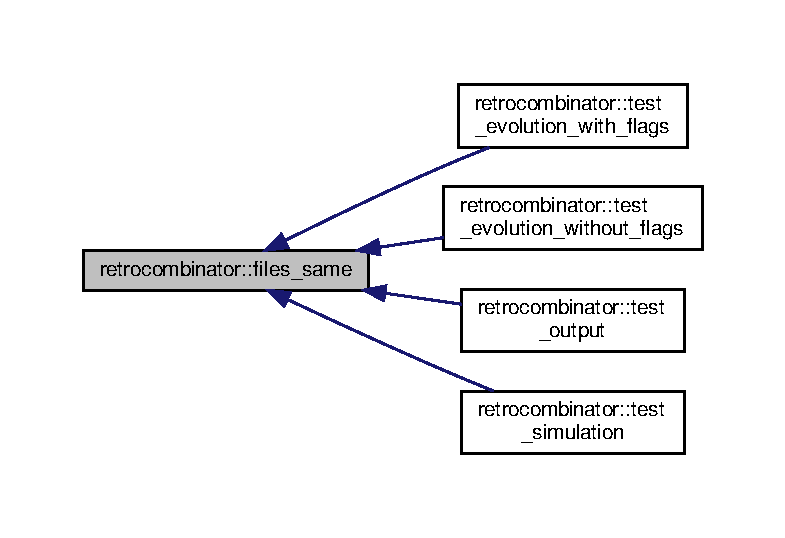
\includegraphics[width=350pt]{namespaceretrocombinator_aadb27262663ae58fda77172ae3d828dc_icgraph}
\end{center}
\end{figure}
\mbox{\Hypertarget{namespaceretrocombinator_a0e4387f4392819cd377c71d5771b39b1}\label{namespaceretrocombinator_a0e4387f4392819cd377c71d5771b39b1}} 
\index{retrocombinator@{retrocombinator}!matrix\+\_\+equal@{matrix\+\_\+equal}}
\index{matrix\+\_\+equal@{matrix\+\_\+equal}!retrocombinator@{retrocombinator}}
\subsubsection{\texorpdfstring{matrix\+\_\+equal()}{matrix\_equal()}}
{\footnotesize\ttfamily bool retrocombinator\+::matrix\+\_\+equal (\begin{DoxyParamCaption}\item[{const double}]{mat1\mbox{[}$\,$\mbox{]}\mbox{[}\+Consts\+::\+N\+U\+C\+\_\+\+C\+O\+U\+N\+T\mbox{]},  }\item[{const double}]{mat2\mbox{[}$\,$\mbox{]}\mbox{[}\+Consts\+::\+N\+U\+C\+\_\+\+C\+O\+U\+N\+T\mbox{]} }\end{DoxyParamCaption})}



Checks if two probability matrices are equal. 

Since this compares floating point values, it uses some tolerance. Here is the caller graph for this function\+:
\nopagebreak
\begin{figure}[H]
\begin{center}
\leavevmode
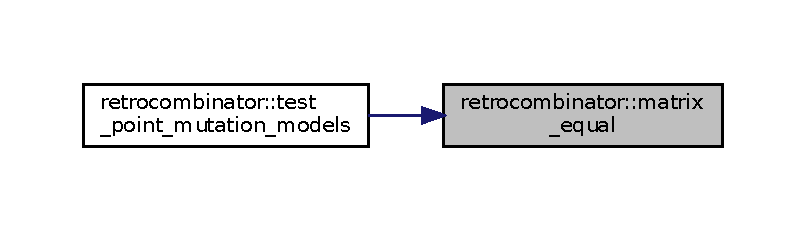
\includegraphics[width=350pt]{namespaceretrocombinator_a0e4387f4392819cd377c71d5771b39b1_icgraph}
\end{center}
\end{figure}
\mbox{\Hypertarget{namespaceretrocombinator_a08dcf1f00c5ea301ff04e3389ed9b3e1}\label{namespaceretrocombinator_a08dcf1f00c5ea301ff04e3389ed9b3e1}} 
\index{retrocombinator@{retrocombinator}!operator\%@{operator\%}}
\index{operator\%@{operator\%}!retrocombinator@{retrocombinator}}
\subsubsection{\texorpdfstring{operator\%()}{operator\%()}\hspace{0.1cm}{\footnotesize\ttfamily [1/2]}}
{\footnotesize\ttfamily double retrocombinator\+::operator\% (\begin{DoxyParamCaption}\item[{const \hyperlink{classretrocombinator_1_1Sequence}{Sequence} \&}]{s1,  }\item[{const \hyperlink{classretrocombinator_1_1Sequence}{Sequence} \&}]{s2 }\end{DoxyParamCaption})}

Similarity is 100-\/dissimilarity. Here is the call graph for this function\+:
\nopagebreak
\begin{figure}[H]
\begin{center}
\leavevmode
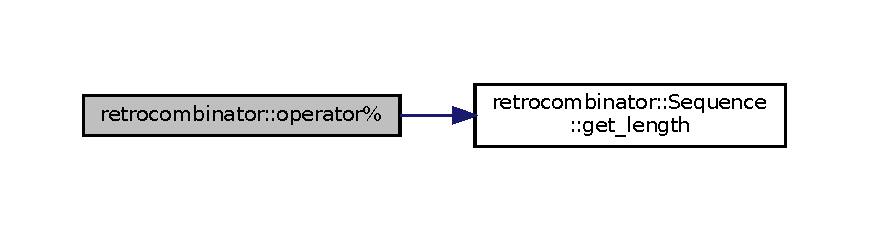
\includegraphics[width=350pt]{namespaceretrocombinator_a08dcf1f00c5ea301ff04e3389ed9b3e1_cgraph}
\end{center}
\end{figure}
\mbox{\Hypertarget{namespaceretrocombinator_a540b38522d54f6df8c0b7d9541b287c7}\label{namespaceretrocombinator_a540b38522d54f6df8c0b7d9541b287c7}} 
\index{retrocombinator@{retrocombinator}!operator\%@{operator\%}}
\index{operator\%@{operator\%}!retrocombinator@{retrocombinator}}
\subsubsection{\texorpdfstring{operator\%()}{operator\%()}\hspace{0.1cm}{\footnotesize\ttfamily [2/2]}}
{\footnotesize\ttfamily double retrocombinator\+::operator\% (\begin{DoxyParamCaption}\item[{const \hyperlink{classretrocombinator_1_1Sequence}{Sequence} \&}]{s1,  }\item[{std\+::string}]{s2 }\end{DoxyParamCaption})}

Similarity is 100-\/dissimilarity. Here is the call graph for this function\+:
\nopagebreak
\begin{figure}[H]
\begin{center}
\leavevmode
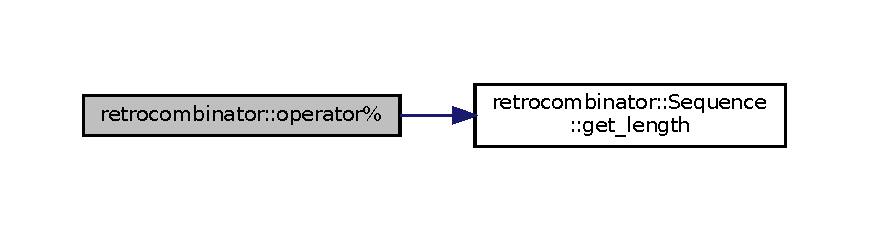
\includegraphics[width=350pt]{namespaceretrocombinator_a540b38522d54f6df8c0b7d9541b287c7_cgraph}
\end{center}
\end{figure}
\mbox{\Hypertarget{namespaceretrocombinator_a2d223ac406c9e02cf5687c709ad5da9d}\label{namespaceretrocombinator_a2d223ac406c9e02cf5687c709ad5da9d}} 
\index{retrocombinator@{retrocombinator}!operator$\ast$@{operator$\ast$}}
\index{operator$\ast$@{operator$\ast$}!retrocombinator@{retrocombinator}}
\subsubsection{\texorpdfstring{operator$\ast$()}{operator*()}\hspace{0.1cm}{\footnotesize\ttfamily [1/2]}}
{\footnotesize\ttfamily \hyperlink{namespaceretrocombinator_a8e1541b50cee66a791df4c437ccbb385}{size\+\_\+type} retrocombinator\+::operator$\ast$ (\begin{DoxyParamCaption}\item[{const \hyperlink{classretrocombinator_1_1Sequence}{Sequence} \&}]{s1,  }\item[{const \hyperlink{classretrocombinator_1_1Sequence}{Sequence} \&}]{s2 }\end{DoxyParamCaption})}

This is the standard edit distance score, and is the number of mismatches (because insertions and deletions are not possible in this system). Here is the call graph for this function\+:
\nopagebreak
\begin{figure}[H]
\begin{center}
\leavevmode
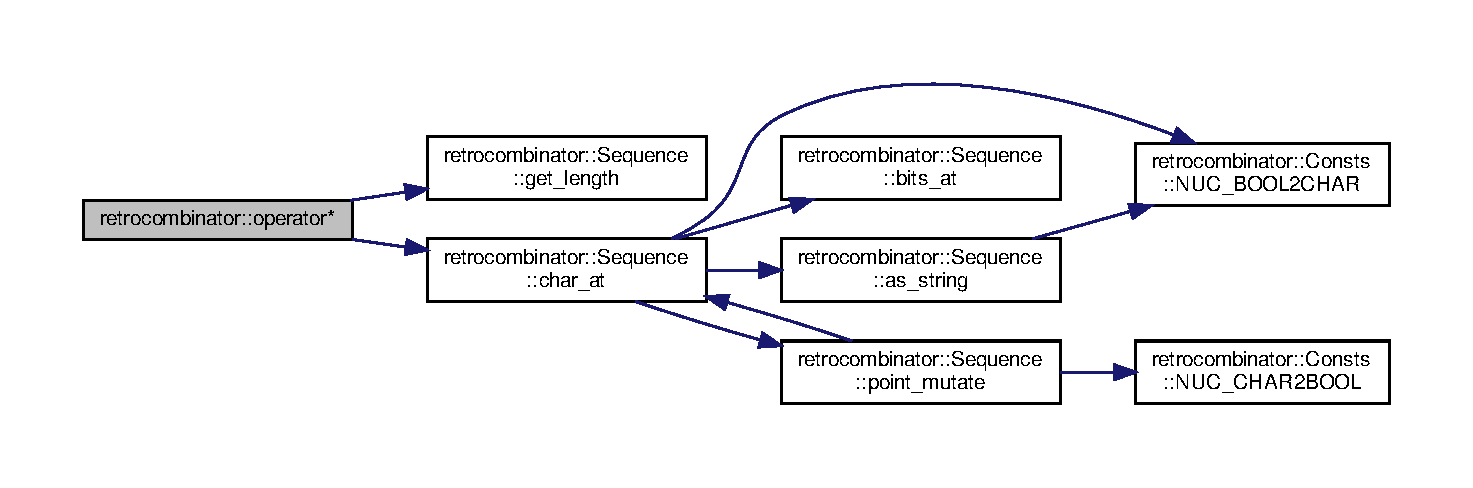
\includegraphics[width=350pt]{namespaceretrocombinator_a2d223ac406c9e02cf5687c709ad5da9d_cgraph}
\end{center}
\end{figure}
\mbox{\Hypertarget{namespaceretrocombinator_a33fa303439100639ad5432a19b8c01d4}\label{namespaceretrocombinator_a33fa303439100639ad5432a19b8c01d4}} 
\index{retrocombinator@{retrocombinator}!operator$\ast$@{operator$\ast$}}
\index{operator$\ast$@{operator$\ast$}!retrocombinator@{retrocombinator}}
\subsubsection{\texorpdfstring{operator$\ast$()}{operator*()}\hspace{0.1cm}{\footnotesize\ttfamily [2/2]}}
{\footnotesize\ttfamily \hyperlink{namespaceretrocombinator_a8e1541b50cee66a791df4c437ccbb385}{size\+\_\+type} retrocombinator\+::operator$\ast$ (\begin{DoxyParamCaption}\item[{const \hyperlink{classretrocombinator_1_1Sequence}{Sequence} \&}]{s1,  }\item[{std\+::string}]{s2 }\end{DoxyParamCaption})}

This is the standard edit distance score, and is the number of mismatches (because insertions and deletions are not possible in this system). Here is the call graph for this function\+:
\nopagebreak
\begin{figure}[H]
\begin{center}
\leavevmode
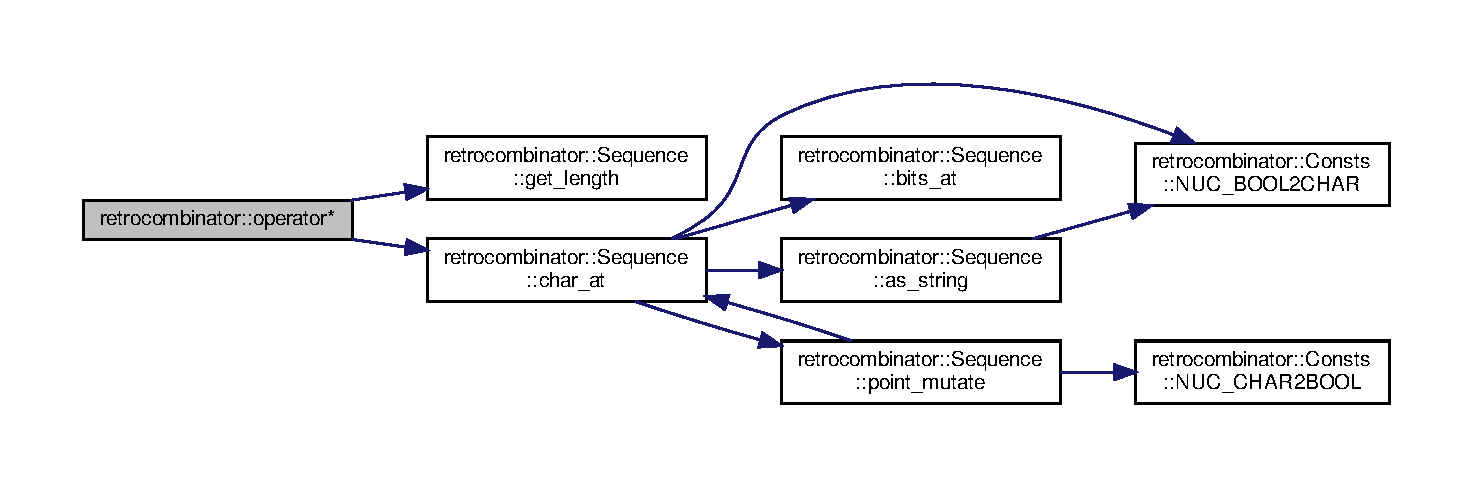
\includegraphics[width=350pt]{namespaceretrocombinator_a33fa303439100639ad5432a19b8c01d4_cgraph}
\end{center}
\end{figure}
\mbox{\Hypertarget{namespaceretrocombinator_a3d34bdb68843d370ccb2374dfb8e9eac}\label{namespaceretrocombinator_a3d34bdb68843d370ccb2374dfb8e9eac}} 
\index{retrocombinator@{retrocombinator}!simulate\+\_\+with\+\_\+flags@{simulate\+\_\+with\+\_\+flags}}
\index{simulate\+\_\+with\+\_\+flags@{simulate\+\_\+with\+\_\+flags}!retrocombinator@{retrocombinator}}
\subsubsection{\texorpdfstring{simulate\+\_\+with\+\_\+flags()}{simulate\_with\_flags()}\hspace{0.1cm}{\footnotesize\ttfamily [1/2]}}
{\footnotesize\ttfamily void retrocombinator\+::simulate\+\_\+with\+\_\+flags (\begin{DoxyParamCaption}\item[{std\+::vector$<$ std\+::string $>$}]{init\+\_\+seqs,  }\item[{\hyperlink{namespaceretrocombinator_a8e1541b50cee66a791df4c437ccbb385}{size\+\_\+type}}]{init\+\_\+seq\+\_\+index,  }\item[{std\+::string}]{point\+\_\+mutation\+\_\+model,  }\item[{\hyperlink{namespaceretrocombinator_a8e1541b50cee66a791df4c437ccbb385}{size\+\_\+type}}]{num\+\_\+sensitive\+\_\+posns,  }\item[{double}]{inactive\+\_\+probability,  }\item[{\hyperlink{namespaceretrocombinator_a8e1541b50cee66a791df4c437ccbb385}{size\+\_\+type}}]{num\+\_\+jumps,  }\item[{double}]{timestep,  }\item[{double}]{burst\+\_\+probability,  }\item[{double}]{burst\+\_\+mean,  }\item[{\hyperlink{namespaceretrocombinator_a8e1541b50cee66a791df4c437ccbb385}{size\+\_\+type}}]{max\+\_\+active\+\_\+copies,  }\item[{\hyperlink{namespaceretrocombinator_a8e1541b50cee66a791df4c437ccbb385}{size\+\_\+type}}]{max\+\_\+total\+\_\+copies,  }\item[{double}]{recomb\+\_\+mean,  }\item[{double}]{selection\+\_\+threshold,  }\item[{double}]{fam\+\_\+proportion,  }\item[{double}]{fam\+\_\+percentage,  }\item[{std\+::string}]{file\+\_\+out,  }\item[{\hyperlink{namespaceretrocombinator_a8e1541b50cee66a791df4c437ccbb385}{size\+\_\+type}}]{num\+\_\+out\+\_\+tags,  }\item[{\hyperlink{namespaceretrocombinator_a8e1541b50cee66a791df4c437ccbb385}{size\+\_\+type}}]{num\+\_\+out\+\_\+init,  }\item[{\hyperlink{namespaceretrocombinator_a8e1541b50cee66a791df4c437ccbb385}{size\+\_\+type}}]{num\+\_\+out\+\_\+seqs,  }\item[{\hyperlink{namespaceretrocombinator_a8e1541b50cee66a791df4c437ccbb385}{size\+\_\+type}}]{num\+\_\+out\+\_\+pair,  }\item[{bool}]{to\+\_\+randomise,  }\item[{bool}]{to\+\_\+seed,  }\item[{\hyperlink{namespaceretrocombinator_a8e1541b50cee66a791df4c437ccbb385}{size\+\_\+type}}]{seed,  }\item[{\hyperlink{namespaceretrocombinator_a8e1541b50cee66a791df4c437ccbb385}{size\+\_\+type}}]{sequence\+\_\+numbering,  }\item[{\hyperlink{namespaceretrocombinator_a8e1541b50cee66a791df4c437ccbb385}{size\+\_\+type}}]{family\+\_\+numbering }\end{DoxyParamCaption})}



Sets up and runs a simulation with flags. 

Takes a specified set of initial sequences. Here is the call graph for this function\+:
\nopagebreak
\begin{figure}[H]
\begin{center}
\leavevmode
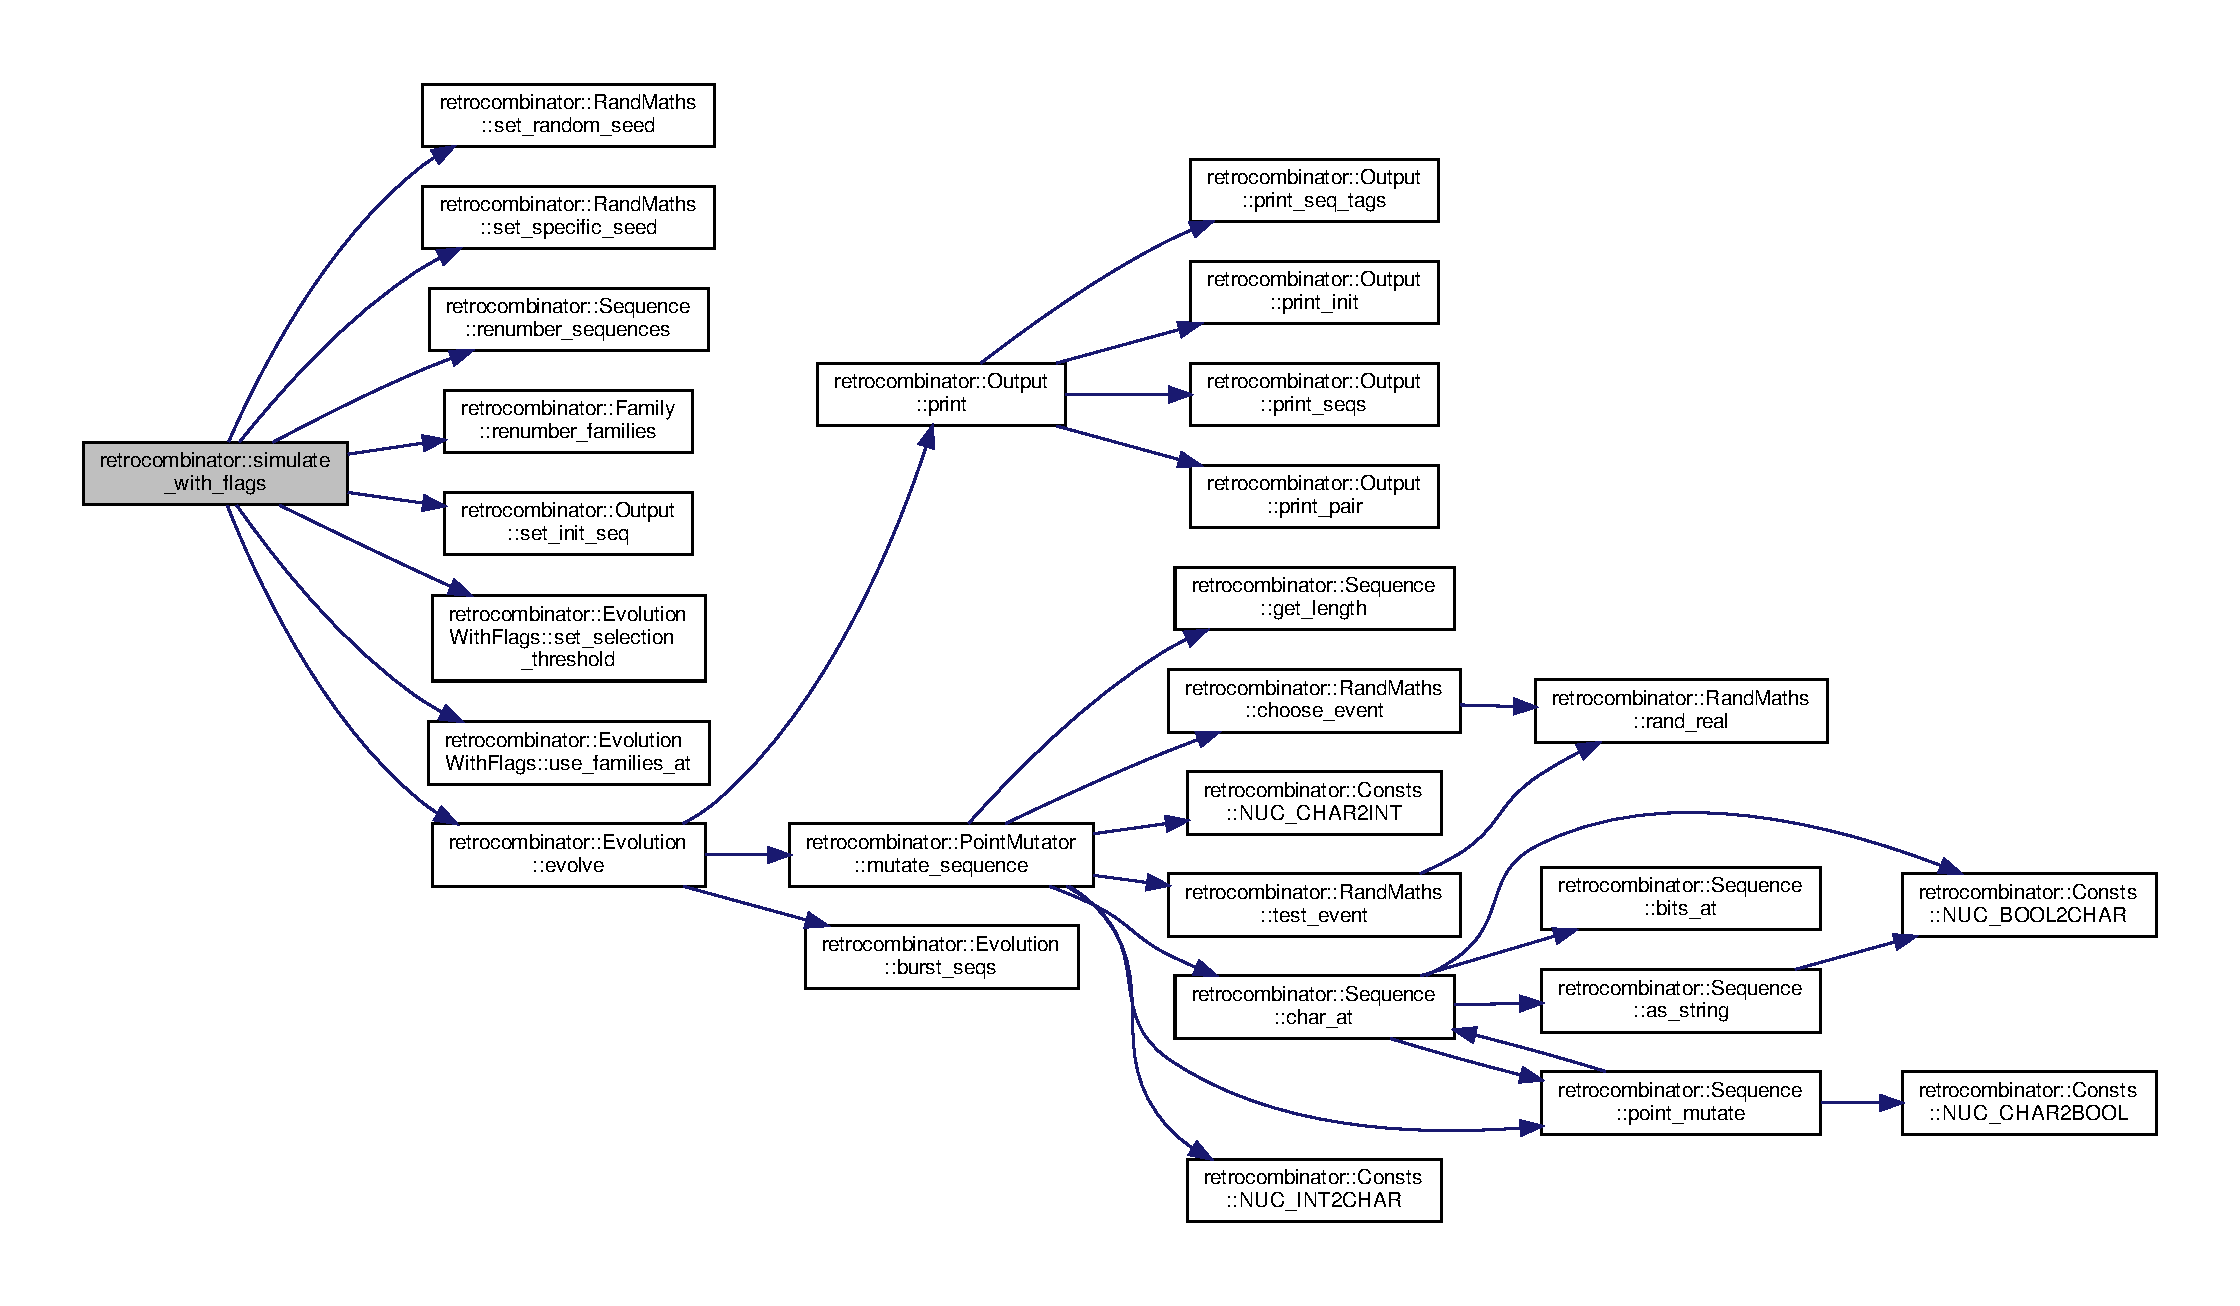
\includegraphics[width=350pt]{namespaceretrocombinator_a3d34bdb68843d370ccb2374dfb8e9eac_cgraph}
\end{center}
\end{figure}
Here is the caller graph for this function\+:
\nopagebreak
\begin{figure}[H]
\begin{center}
\leavevmode
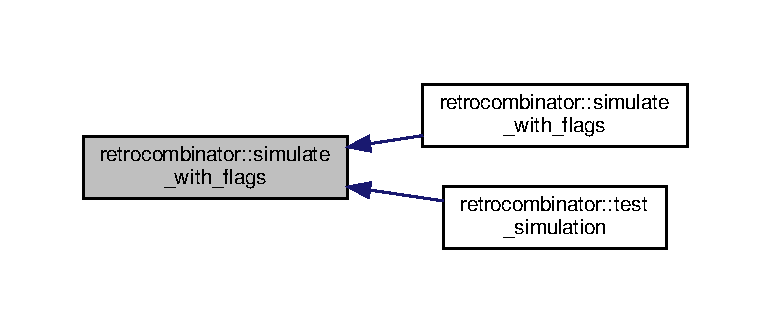
\includegraphics[width=350pt]{namespaceretrocombinator_a3d34bdb68843d370ccb2374dfb8e9eac_icgraph}
\end{center}
\end{figure}
\mbox{\Hypertarget{namespaceretrocombinator_a3875c27225976a6e04bde555c3acca36}\label{namespaceretrocombinator_a3875c27225976a6e04bde555c3acca36}} 
\index{retrocombinator@{retrocombinator}!simulate\+\_\+with\+\_\+flags@{simulate\+\_\+with\+\_\+flags}}
\index{simulate\+\_\+with\+\_\+flags@{simulate\+\_\+with\+\_\+flags}!retrocombinator@{retrocombinator}}
\subsubsection{\texorpdfstring{simulate\+\_\+with\+\_\+flags()}{simulate\_with\_flags()}\hspace{0.1cm}{\footnotesize\ttfamily [2/2]}}
{\footnotesize\ttfamily void retrocombinator\+::simulate\+\_\+with\+\_\+flags (\begin{DoxyParamCaption}\item[{\hyperlink{namespaceretrocombinator_a8e1541b50cee66a791df4c437ccbb385}{size\+\_\+type}}]{num\+\_\+seq,  }\item[{\hyperlink{namespaceretrocombinator_a8e1541b50cee66a791df4c437ccbb385}{size\+\_\+type}}]{seq\+\_\+length,  }\item[{std\+::string}]{point\+\_\+mutation\+\_\+model,  }\item[{\hyperlink{namespaceretrocombinator_a8e1541b50cee66a791df4c437ccbb385}{size\+\_\+type}}]{num\+\_\+sensitive\+\_\+posns,  }\item[{double}]{inactive\+\_\+probability,  }\item[{\hyperlink{namespaceretrocombinator_a8e1541b50cee66a791df4c437ccbb385}{size\+\_\+type}}]{num\+\_\+jumps,  }\item[{double}]{timestep,  }\item[{double}]{burst\+\_\+probability,  }\item[{double}]{burst\+\_\+mean,  }\item[{\hyperlink{namespaceretrocombinator_a8e1541b50cee66a791df4c437ccbb385}{size\+\_\+type}}]{max\+\_\+active\+\_\+copies,  }\item[{\hyperlink{namespaceretrocombinator_a8e1541b50cee66a791df4c437ccbb385}{size\+\_\+type}}]{max\+\_\+total\+\_\+copies,  }\item[{double}]{recomb\+\_\+mean,  }\item[{double}]{selection\+\_\+threshold,  }\item[{double}]{fam\+\_\+proportion,  }\item[{double}]{fam\+\_\+percentage,  }\item[{std\+::string}]{file\+\_\+out,  }\item[{\hyperlink{namespaceretrocombinator_a8e1541b50cee66a791df4c437ccbb385}{size\+\_\+type}}]{num\+\_\+out\+\_\+tags,  }\item[{\hyperlink{namespaceretrocombinator_a8e1541b50cee66a791df4c437ccbb385}{size\+\_\+type}}]{num\+\_\+out\+\_\+init,  }\item[{\hyperlink{namespaceretrocombinator_a8e1541b50cee66a791df4c437ccbb385}{size\+\_\+type}}]{num\+\_\+out\+\_\+seqs,  }\item[{\hyperlink{namespaceretrocombinator_a8e1541b50cee66a791df4c437ccbb385}{size\+\_\+type}}]{num\+\_\+out\+\_\+pair,  }\item[{bool}]{to\+\_\+randomise,  }\item[{bool}]{to\+\_\+seed,  }\item[{\hyperlink{namespaceretrocombinator_a8e1541b50cee66a791df4c437ccbb385}{size\+\_\+type}}]{seed,  }\item[{\hyperlink{namespaceretrocombinator_a8e1541b50cee66a791df4c437ccbb385}{size\+\_\+type}}]{sequence\+\_\+numbering,  }\item[{\hyperlink{namespaceretrocombinator_a8e1541b50cee66a791df4c437ccbb385}{size\+\_\+type}}]{family\+\_\+numbering }\end{DoxyParamCaption})}



Sets up and runs a simulation with flags. 

Constructs initial sequences randomly. Here is the call graph for this function\+:
\nopagebreak
\begin{figure}[H]
\begin{center}
\leavevmode
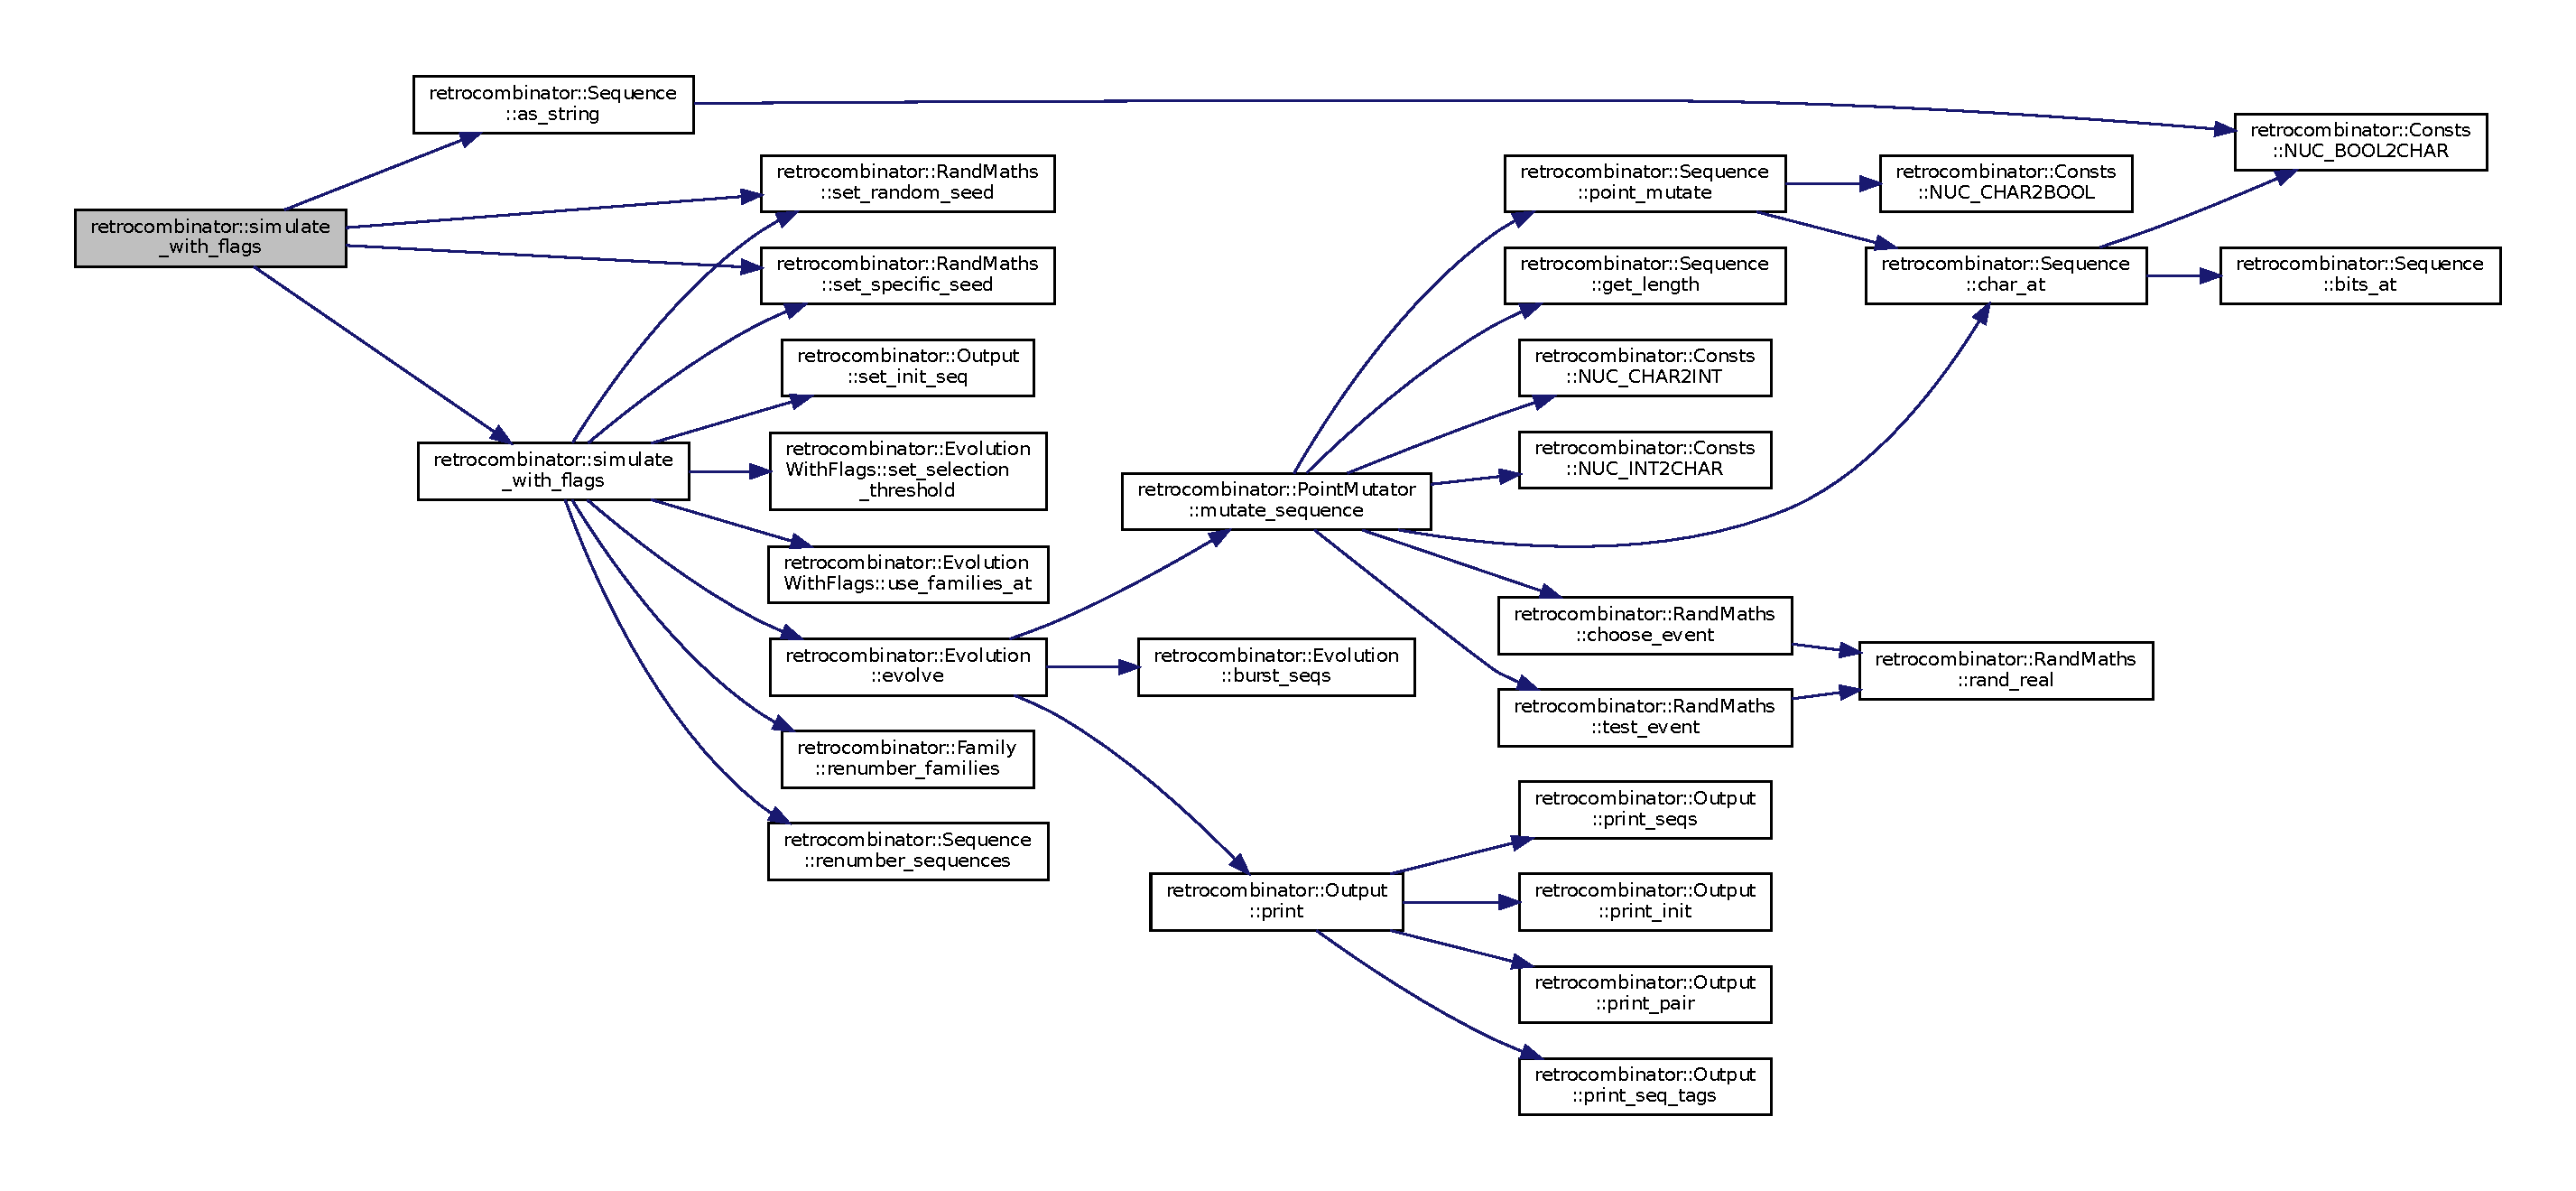
\includegraphics[width=350pt]{namespaceretrocombinator_a3875c27225976a6e04bde555c3acca36_cgraph}
\end{center}
\end{figure}
\mbox{\Hypertarget{namespaceretrocombinator_ab4bb894621063b932d80c1473b359534}\label{namespaceretrocombinator_ab4bb894621063b932d80c1473b359534}} 
\index{retrocombinator@{retrocombinator}!simulate\+\_\+without\+\_\+flags@{simulate\+\_\+without\+\_\+flags}}
\index{simulate\+\_\+without\+\_\+flags@{simulate\+\_\+without\+\_\+flags}!retrocombinator@{retrocombinator}}
\subsubsection{\texorpdfstring{simulate\+\_\+without\+\_\+flags()}{simulate\_without\_flags()}\hspace{0.1cm}{\footnotesize\ttfamily [1/2]}}
{\footnotesize\ttfamily void retrocombinator\+::simulate\+\_\+without\+\_\+flags (\begin{DoxyParamCaption}\item[{std\+::vector$<$ std\+::string $>$}]{init\+\_\+seqs,  }\item[{\hyperlink{namespaceretrocombinator_a8e1541b50cee66a791df4c437ccbb385}{size\+\_\+type}}]{init\+\_\+seq\+\_\+index,  }\item[{std\+::string}]{point\+\_\+mutation\+\_\+model,  }\item[{\hyperlink{namespaceretrocombinator_a8e1541b50cee66a791df4c437ccbb385}{size\+\_\+type}}]{num\+\_\+jumps,  }\item[{double}]{timestep,  }\item[{double}]{burst\+\_\+probability,  }\item[{double}]{burst\+\_\+mean,  }\item[{\hyperlink{namespaceretrocombinator_a8e1541b50cee66a791df4c437ccbb385}{size\+\_\+type}}]{max\+\_\+active\+\_\+copies,  }\item[{double}]{recomb\+\_\+mean,  }\item[{std\+::string}]{file\+\_\+out,  }\item[{\hyperlink{namespaceretrocombinator_a8e1541b50cee66a791df4c437ccbb385}{size\+\_\+type}}]{num\+\_\+out\+\_\+tags,  }\item[{\hyperlink{namespaceretrocombinator_a8e1541b50cee66a791df4c437ccbb385}{size\+\_\+type}}]{num\+\_\+out\+\_\+init,  }\item[{\hyperlink{namespaceretrocombinator_a8e1541b50cee66a791df4c437ccbb385}{size\+\_\+type}}]{num\+\_\+out\+\_\+seqs,  }\item[{\hyperlink{namespaceretrocombinator_a8e1541b50cee66a791df4c437ccbb385}{size\+\_\+type}}]{num\+\_\+out\+\_\+pair,  }\item[{bool}]{to\+\_\+randomise,  }\item[{bool}]{to\+\_\+seed,  }\item[{\hyperlink{namespaceretrocombinator_a8e1541b50cee66a791df4c437ccbb385}{size\+\_\+type}}]{seed,  }\item[{\hyperlink{namespaceretrocombinator_a8e1541b50cee66a791df4c437ccbb385}{size\+\_\+type}}]{sequence\+\_\+numbering,  }\item[{\hyperlink{namespaceretrocombinator_a8e1541b50cee66a791df4c437ccbb385}{size\+\_\+type}}]{family\+\_\+numbering }\end{DoxyParamCaption})}



Sets up and runs a simulation without flags. 

Takes a specified set of initial sequences. Here is the call graph for this function\+:
\nopagebreak
\begin{figure}[H]
\begin{center}
\leavevmode
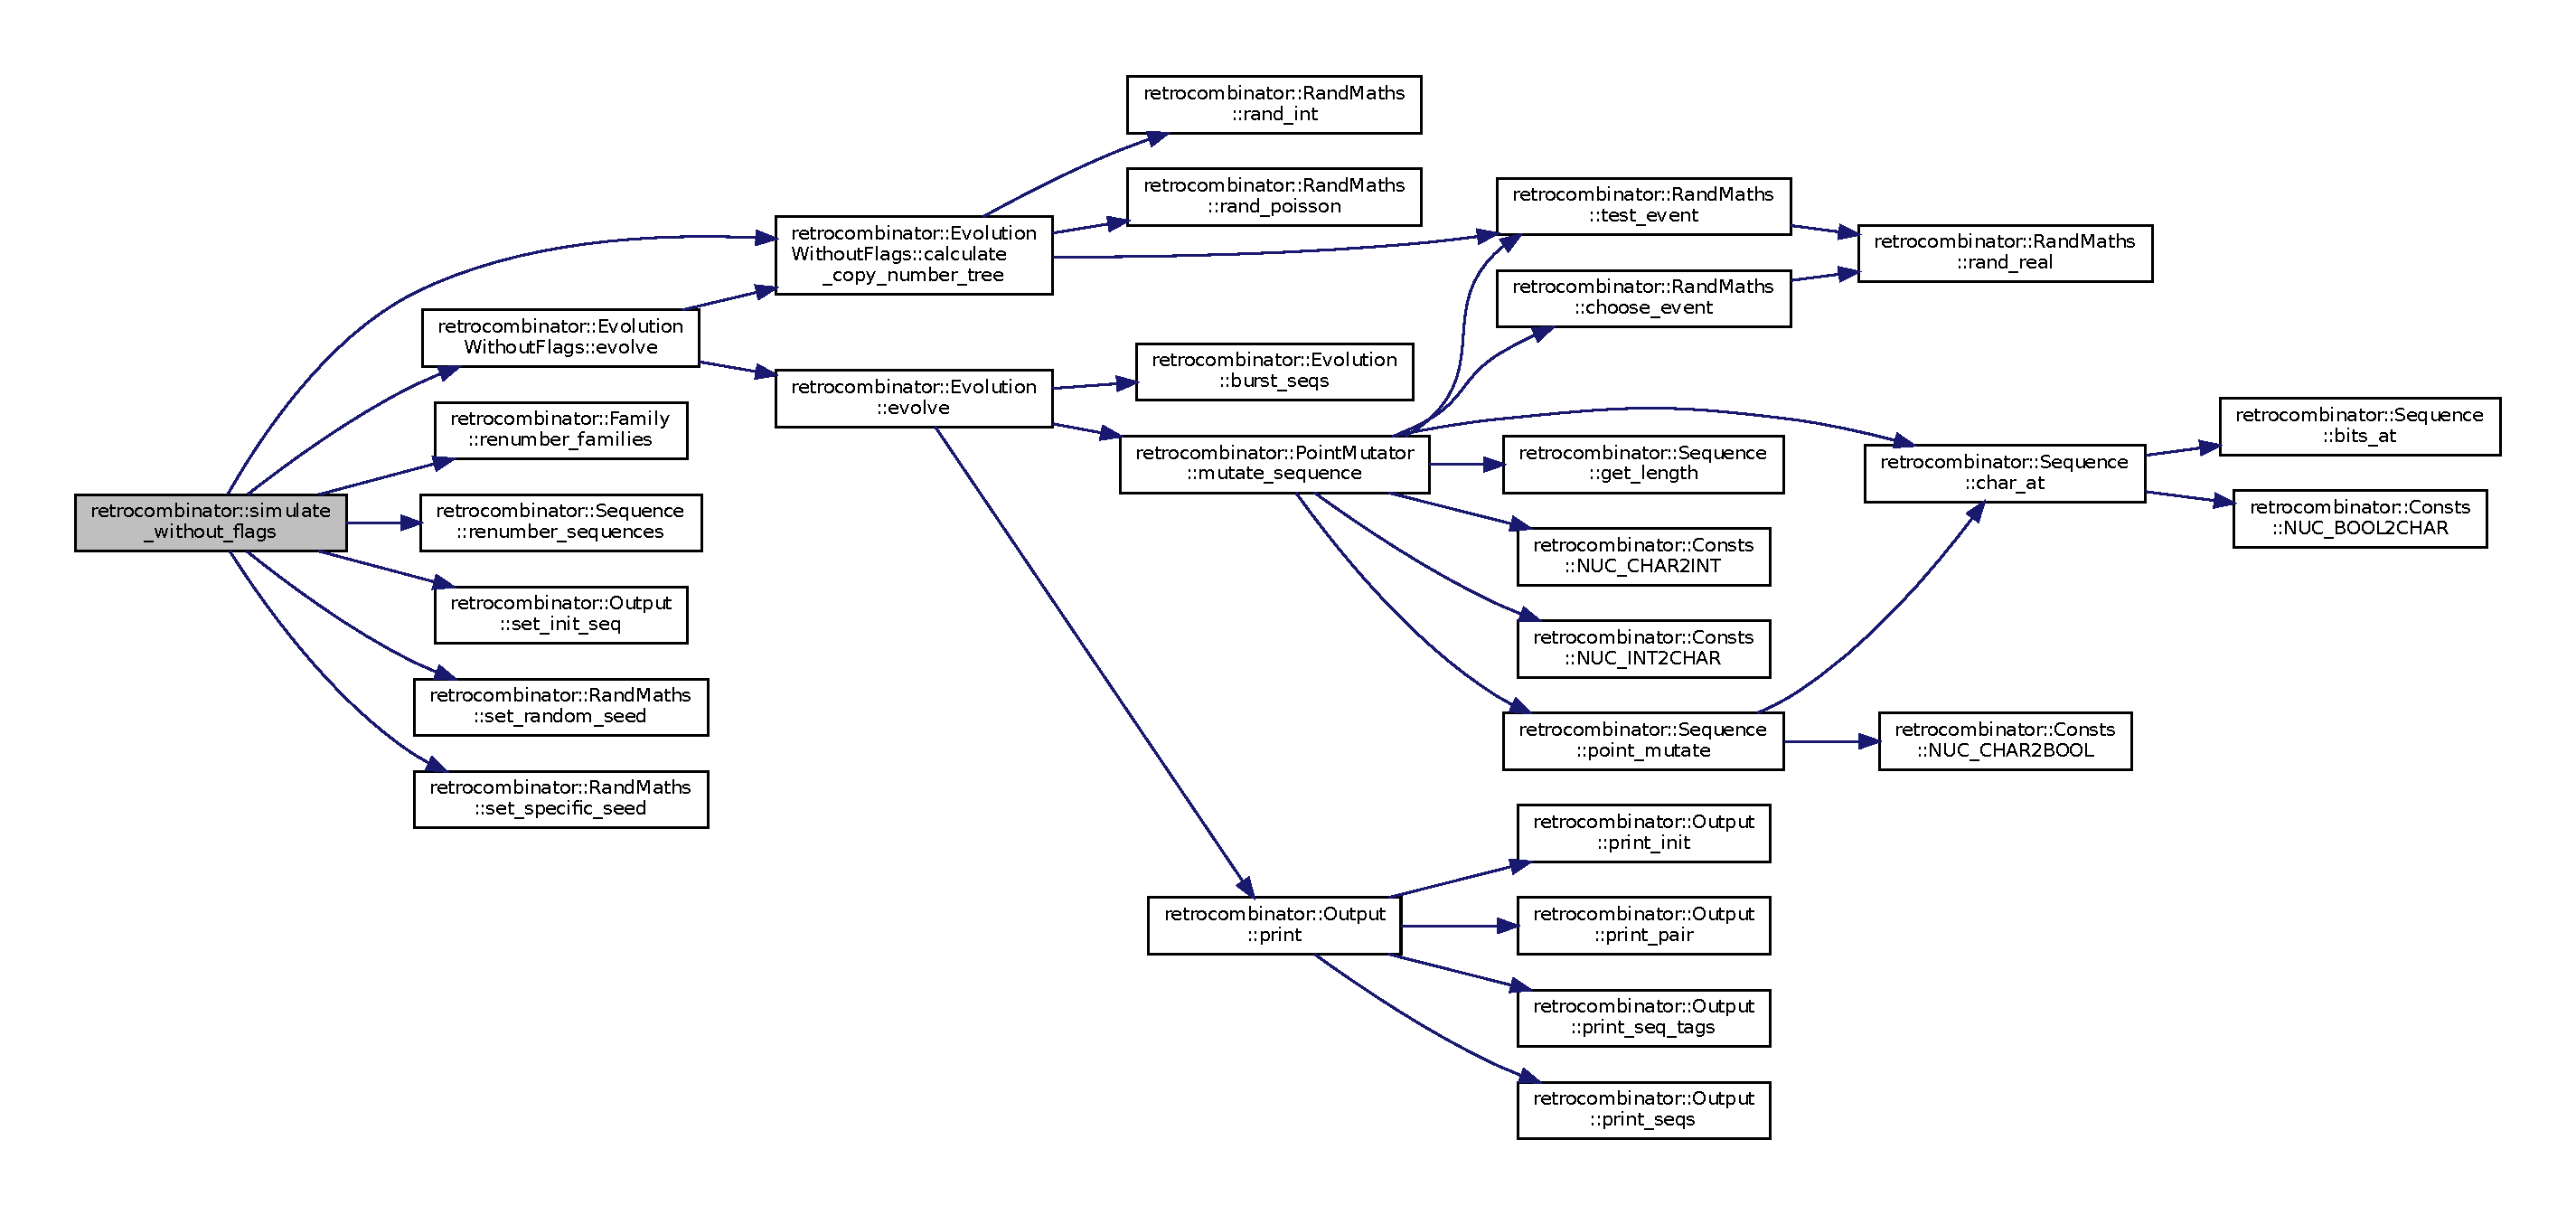
\includegraphics[width=350pt]{namespaceretrocombinator_ab4bb894621063b932d80c1473b359534_cgraph}
\end{center}
\end{figure}
Here is the caller graph for this function\+:
\nopagebreak
\begin{figure}[H]
\begin{center}
\leavevmode
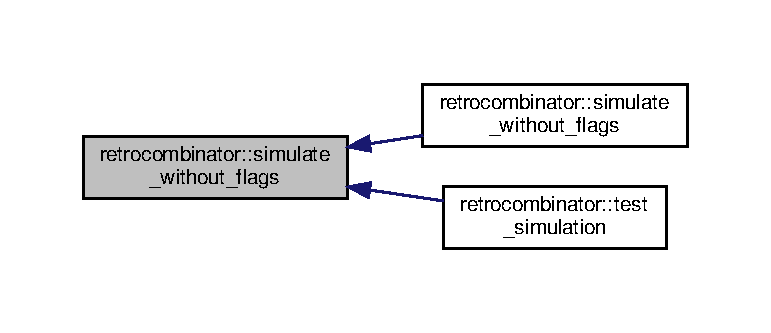
\includegraphics[width=350pt]{namespaceretrocombinator_ab4bb894621063b932d80c1473b359534_icgraph}
\end{center}
\end{figure}
\mbox{\Hypertarget{namespaceretrocombinator_a0dc31e2b9d6473e995395d8171f56312}\label{namespaceretrocombinator_a0dc31e2b9d6473e995395d8171f56312}} 
\index{retrocombinator@{retrocombinator}!simulate\+\_\+without\+\_\+flags@{simulate\+\_\+without\+\_\+flags}}
\index{simulate\+\_\+without\+\_\+flags@{simulate\+\_\+without\+\_\+flags}!retrocombinator@{retrocombinator}}
\subsubsection{\texorpdfstring{simulate\+\_\+without\+\_\+flags()}{simulate\_without\_flags()}\hspace{0.1cm}{\footnotesize\ttfamily [2/2]}}
{\footnotesize\ttfamily void retrocombinator\+::simulate\+\_\+without\+\_\+flags (\begin{DoxyParamCaption}\item[{\hyperlink{namespaceretrocombinator_a8e1541b50cee66a791df4c437ccbb385}{size\+\_\+type}}]{num\+\_\+seq,  }\item[{\hyperlink{namespaceretrocombinator_a8e1541b50cee66a791df4c437ccbb385}{size\+\_\+type}}]{seq\+\_\+length,  }\item[{std\+::string}]{point\+\_\+mutation\+\_\+model,  }\item[{\hyperlink{namespaceretrocombinator_a8e1541b50cee66a791df4c437ccbb385}{size\+\_\+type}}]{num\+\_\+jumps,  }\item[{double}]{timestep,  }\item[{double}]{burst\+\_\+probability,  }\item[{double}]{burst\+\_\+mean,  }\item[{\hyperlink{namespaceretrocombinator_a8e1541b50cee66a791df4c437ccbb385}{size\+\_\+type}}]{max\+\_\+active\+\_\+copies,  }\item[{double}]{recomb\+\_\+mean,  }\item[{std\+::string}]{file\+\_\+out,  }\item[{\hyperlink{namespaceretrocombinator_a8e1541b50cee66a791df4c437ccbb385}{size\+\_\+type}}]{num\+\_\+out\+\_\+tags,  }\item[{\hyperlink{namespaceretrocombinator_a8e1541b50cee66a791df4c437ccbb385}{size\+\_\+type}}]{num\+\_\+out\+\_\+init,  }\item[{\hyperlink{namespaceretrocombinator_a8e1541b50cee66a791df4c437ccbb385}{size\+\_\+type}}]{num\+\_\+out\+\_\+seqs,  }\item[{\hyperlink{namespaceretrocombinator_a8e1541b50cee66a791df4c437ccbb385}{size\+\_\+type}}]{num\+\_\+out\+\_\+pair,  }\item[{bool}]{to\+\_\+randomise,  }\item[{bool}]{to\+\_\+seed,  }\item[{\hyperlink{namespaceretrocombinator_a8e1541b50cee66a791df4c437ccbb385}{size\+\_\+type}}]{seed,  }\item[{\hyperlink{namespaceretrocombinator_a8e1541b50cee66a791df4c437ccbb385}{size\+\_\+type}}]{sequence\+\_\+numbering,  }\item[{\hyperlink{namespaceretrocombinator_a8e1541b50cee66a791df4c437ccbb385}{size\+\_\+type}}]{family\+\_\+numbering }\end{DoxyParamCaption})}



Sets up and runs a simulation without flags. 

Constructs initial sequences randomly. Here is the call graph for this function\+:
\nopagebreak
\begin{figure}[H]
\begin{center}
\leavevmode
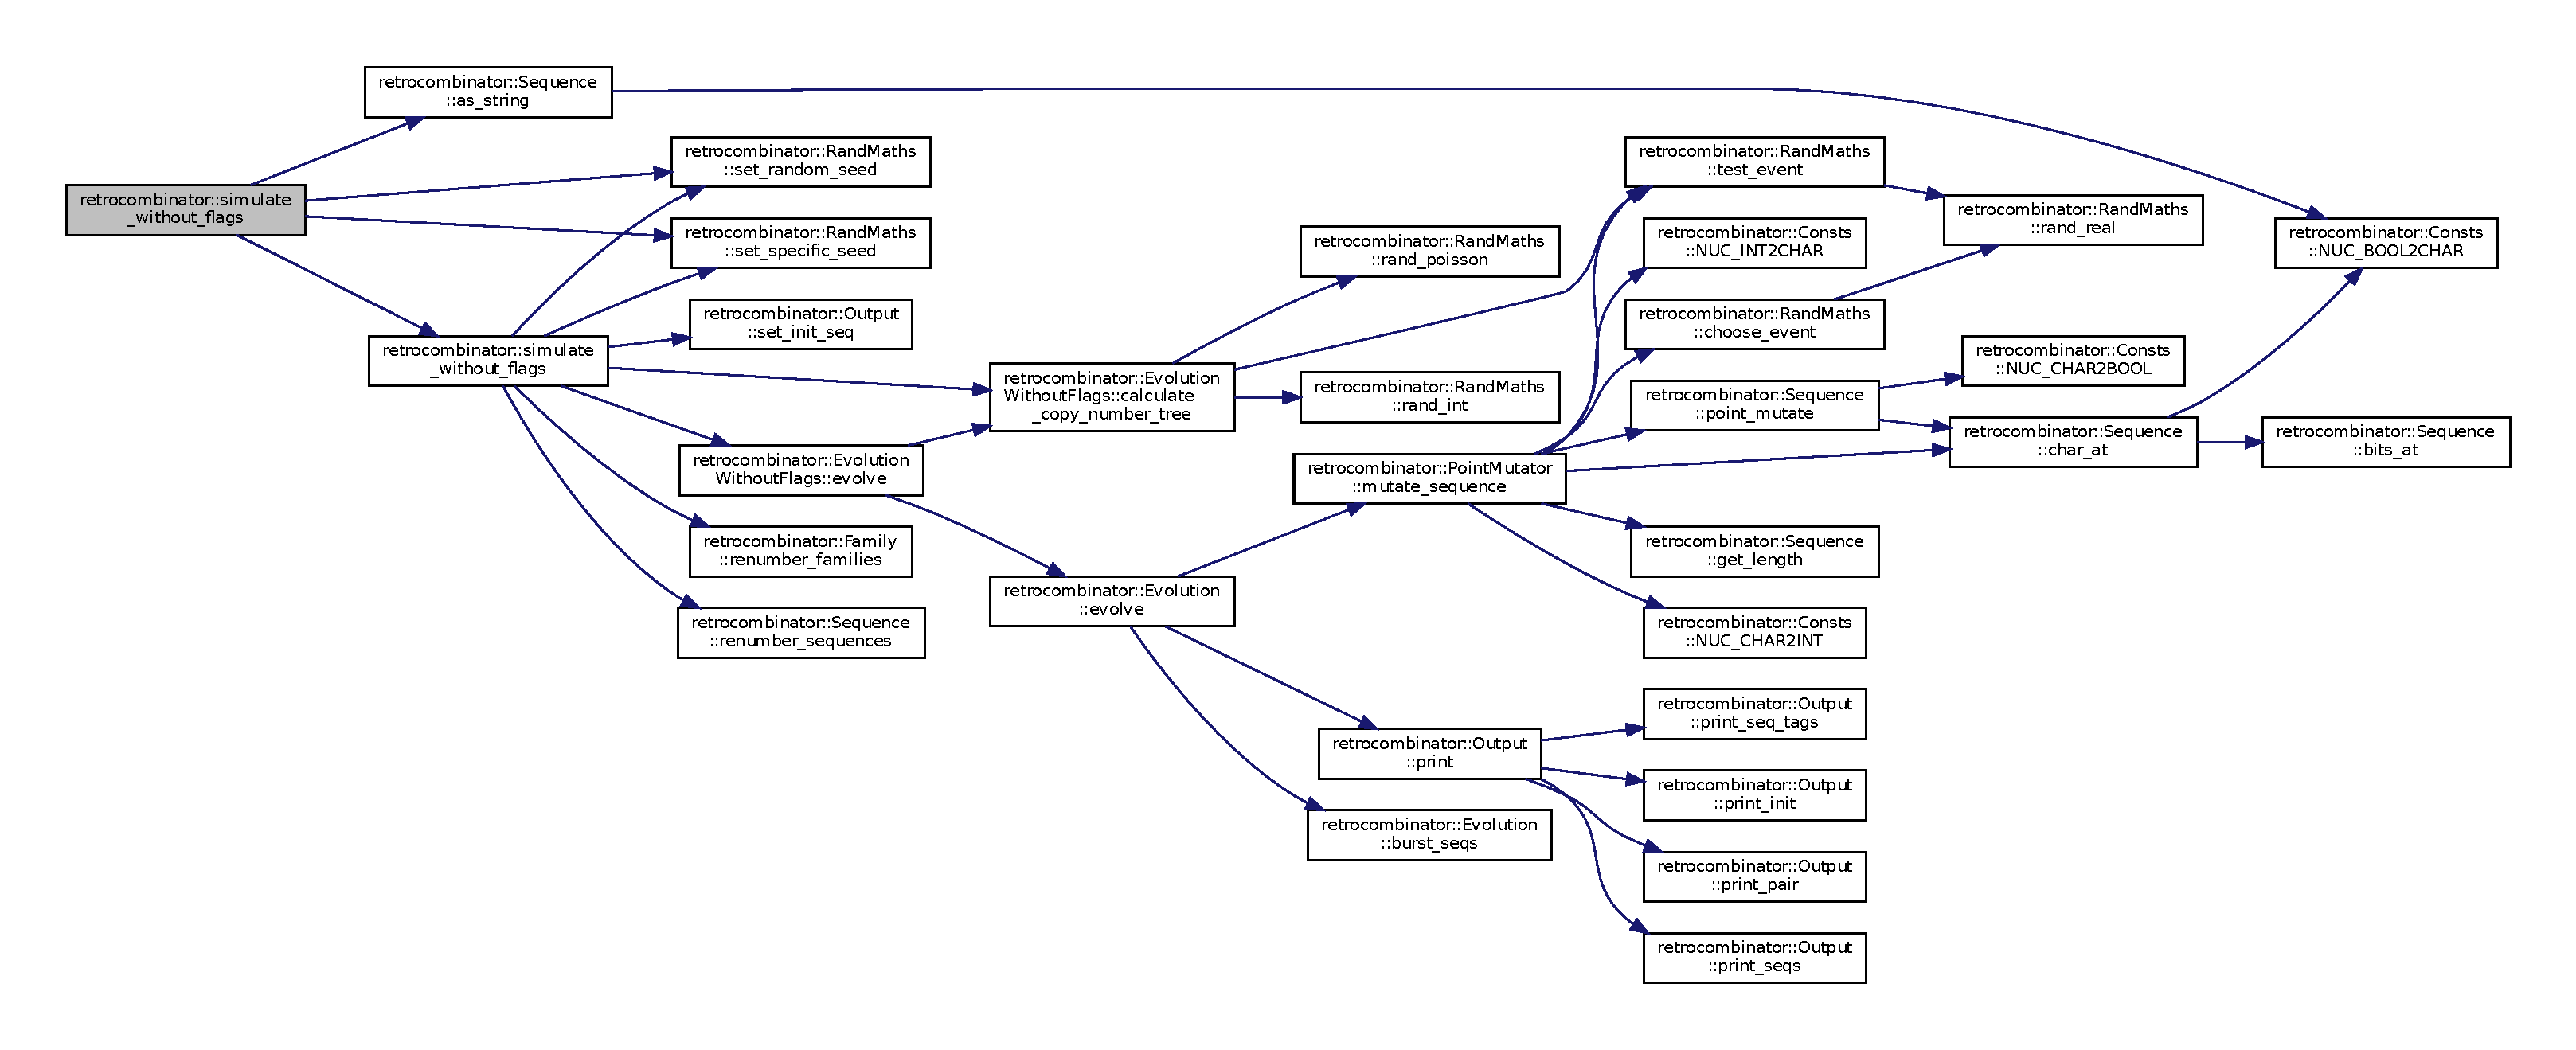
\includegraphics[width=350pt]{namespaceretrocombinator_a0dc31e2b9d6473e995395d8171f56312_cgraph}
\end{center}
\end{figure}


\subsection{Variable Documentation}
\mbox{\Hypertarget{namespaceretrocombinator_a4987db6a228df9ffab41c0a5342556f6}\label{namespaceretrocombinator_a4987db6a228df9ffab41c0a5342556f6}} 
\index{retrocombinator@{retrocombinator}!R\+NG@{R\+NG}}
\index{R\+NG@{R\+NG}!retrocombinator@{retrocombinator}}
\subsubsection{\texorpdfstring{R\+NG}{RNG}}
{\footnotesize\ttfamily \hyperlink{classretrocombinator_1_1RandMaths}{Rand\+Maths} \& retrocombinator\+::\+R\+NG = \hyperlink{classretrocombinator_1_1RandMaths_ae54dee1a16fb0e275e1624ccaa7dc87e}{Rand\+Maths\+::get\+\_\+instance}()}



Global random number generator. 

Used to completely determine the random effects of a simulation by specifying a seed. 
\hypertarget{namespaceretrocombinator_1_1Consts}{}\doxysection{retrocombinator\+::Consts Namespace Reference}
\label{namespaceretrocombinator_1_1Consts}\index{retrocombinator::Consts@{retrocombinator::Consts}}
\doxysubsection*{Enumerations}
\begin{DoxyCompactItemize}
\item 
enum \mbox{\hyperlink{namespaceretrocombinator_1_1Consts_a274e9195aeee16a2bc05c6c2d13da17d}{N\+U\+C\+\_\+\+V\+A\+LS}} \{ \newline
\mbox{\hyperlink{namespaceretrocombinator_1_1Consts_a274e9195aeee16a2bc05c6c2d13da17dac9faac145c86659926a2309d19c35dff}{T}} = 0, 
\mbox{\hyperlink{namespaceretrocombinator_1_1Consts_a274e9195aeee16a2bc05c6c2d13da17da8a12357162a7bf22e8578359a62411c6}{C}} = 1, 
\mbox{\hyperlink{namespaceretrocombinator_1_1Consts_a274e9195aeee16a2bc05c6c2d13da17da6c53f477e84902529dcca14ae060567e}{A}} = 2, 
\mbox{\hyperlink{namespaceretrocombinator_1_1Consts_a274e9195aeee16a2bc05c6c2d13da17da06ef41de5b2c3014ce080d3ecece5c4e}{G}} = 3, 
\newline
\mbox{\hyperlink{namespaceretrocombinator_1_1Consts_a274e9195aeee16a2bc05c6c2d13da17da4267c64ef80aa3023d8e808832e04b4e}{N\+U\+C\+\_\+\+C\+O\+U\+NT}} = 4
 \}
\begin{DoxyCompactList}\small\item\em This defines an ordering on the nucleotides, it is used for arrays and transition matrices that work on nucleotides. \end{DoxyCompactList}\end{DoxyCompactItemize}
\doxysubsection*{Functions}
\begin{DoxyCompactItemize}
\item 
\mbox{\Hypertarget{namespaceretrocombinator_1_1Consts_a4f7296df50158c4273a1c5300c24c2f7}\label{namespaceretrocombinator_1_1Consts_a4f7296df50158c4273a1c5300c24c2f7}} 
char \mbox{\hyperlink{namespaceretrocombinator_1_1Consts_a4f7296df50158c4273a1c5300c24c2f7}{N\+U\+C\+\_\+\+I\+N\+T2\+C\+H\+AR}} (int index)
\begin{DoxyCompactList}\small\item\em Returns a character corresponding a nucleotide given its index. \end{DoxyCompactList}\item 
\mbox{\Hypertarget{namespaceretrocombinator_1_1Consts_a074bd1a42191d4770f74beb2bf228111}\label{namespaceretrocombinator_1_1Consts_a074bd1a42191d4770f74beb2bf228111}} 
int \mbox{\hyperlink{namespaceretrocombinator_1_1Consts_a074bd1a42191d4770f74beb2bf228111}{N\+U\+C\+\_\+\+C\+H\+A\+R2\+I\+NT}} (char nucleotide)
\begin{DoxyCompactList}\small\item\em Returns the index of a nucleotide given its character form. \end{DoxyCompactList}\item 
\mbox{\Hypertarget{namespaceretrocombinator_1_1Consts_a95eb077a2bba2fe988b44e68a3284314}\label{namespaceretrocombinator_1_1Consts_a95eb077a2bba2fe988b44e68a3284314}} 
std\+::pair$<$ bool, bool $>$ \mbox{\hyperlink{namespaceretrocombinator_1_1Consts_a95eb077a2bba2fe988b44e68a3284314}{N\+U\+C\+\_\+\+C\+H\+A\+R2\+B\+O\+OL}} (char nucleotide)
\begin{DoxyCompactList}\small\item\em Returns the 2bit-\/encoding of a nucleotide given its character form. \end{DoxyCompactList}\item 
\mbox{\Hypertarget{namespaceretrocombinator_1_1Consts_af335f61cbdfff27175d7f41cd95d426d}\label{namespaceretrocombinator_1_1Consts_af335f61cbdfff27175d7f41cd95d426d}} 
char \mbox{\hyperlink{namespaceretrocombinator_1_1Consts_af335f61cbdfff27175d7f41cd95d426d}{N\+U\+C\+\_\+\+B\+O\+O\+L2\+C\+H\+AR}} (std\+::pair$<$ bool, bool $>$ bits)
\begin{DoxyCompactList}\small\item\em Returns the character of a nucleotide given its 2bit-\/encoding. \end{DoxyCompactList}\end{DoxyCompactItemize}
\doxysubsection*{Variables}
\begin{DoxyCompactItemize}
\item 
\mbox{\Hypertarget{namespaceretrocombinator_1_1Consts_a2b743049e71f91009273f493c164679a}\label{namespaceretrocombinator_1_1Consts_a2b743049e71f91009273f493c164679a}} 
const double \mbox{\hyperlink{namespaceretrocombinator_1_1Consts_a2b743049e71f91009273f493c164679a}{D\+O\+U\+B\+L\+E\+\_\+\+T\+O\+L\+E\+R\+A\+N\+CE}} = pow(10.\+0, -\/8)
\begin{DoxyCompactList}\small\item\em Tolerance for operations on variables of datatype double. \end{DoxyCompactList}\item 
const double \mbox{\hyperlink{namespaceretrocombinator_1_1Consts_ac72fd4ec7b9dc3b42523a83cd69eaee2}{K80\+\_\+K}} = 10
\begin{DoxyCompactList}\small\item\em Defaults for different point mutation models. \end{DoxyCompactList}\item 
\mbox{\Hypertarget{namespaceretrocombinator_1_1Consts_a49787213bbb5ff96754671440c758270}\label{namespaceretrocombinator_1_1Consts_a49787213bbb5ff96754671440c758270}} 
const double \mbox{\hyperlink{namespaceretrocombinator_1_1Consts_a49787213bbb5ff96754671440c758270}{K80\+\_\+\+S\+C\+A\+LE}} = 0.\+01
\begin{DoxyCompactList}\small\item\em Default scale for a K80 point mutation model. \end{DoxyCompactList}\item 
\mbox{\Hypertarget{namespaceretrocombinator_1_1Consts_aeeeb7201b2611b428004059f329473ba}\label{namespaceretrocombinator_1_1Consts_aeeeb7201b2611b428004059f329473ba}} 
const double \mbox{\hyperlink{namespaceretrocombinator_1_1Consts_aeeeb7201b2611b428004059f329473ba}{J\+C69\+\_\+\+S\+C\+A\+LE}} = 0.\+1
\begin{DoxyCompactList}\small\item\em Default scale for a J\+C69 point mutation model. \end{DoxyCompactList}\item 
\mbox{\Hypertarget{namespaceretrocombinator_1_1Consts_af4adf5f1b75ede326285e110e2acf837}\label{namespaceretrocombinator_1_1Consts_af4adf5f1b75ede326285e110e2acf837}} 
const \mbox{\hyperlink{namespaceretrocombinator_afd7c6eb4293e8c4d12827609a9a34b9b}{tag\+\_\+type}} \mbox{\hyperlink{namespaceretrocombinator_1_1Consts_af4adf5f1b75ede326285e110e2acf837}{I\+N\+I\+T\+\_\+\+F\+A\+M\+I\+L\+Y\+\_\+\+C\+O\+U\+NT}} = -\/1
\begin{DoxyCompactList}\small\item\em The family tag to represent initial sequences in a simulation. \end{DoxyCompactList}\end{DoxyCompactItemize}


\doxysubsection{Detailed Description}
Stores biological constants and constants that are specific to an implementation of the simulation. 

\doxysubsection{Enumeration Type Documentation}
\mbox{\Hypertarget{namespaceretrocombinator_1_1Consts_a274e9195aeee16a2bc05c6c2d13da17d}\label{namespaceretrocombinator_1_1Consts_a274e9195aeee16a2bc05c6c2d13da17d}} 
\index{retrocombinator::Consts@{retrocombinator::Consts}!NUC\_VALS@{NUC\_VALS}}
\index{NUC\_VALS@{NUC\_VALS}!retrocombinator::Consts@{retrocombinator::Consts}}
\doxysubsubsection{\texorpdfstring{NUC\_VALS}{NUC\_VALS}}
{\footnotesize\ttfamily enum \mbox{\hyperlink{namespaceretrocombinator_1_1Consts_a274e9195aeee16a2bc05c6c2d13da17d}{retrocombinator\+::\+Consts\+::\+N\+U\+C\+\_\+\+V\+A\+LS}}}



This defines an ordering on the nucleotides, it is used for arrays and transition matrices that work on nucleotides. 

\begin{DoxyEnumFields}{Enumerator}
\raisebox{\heightof{T}}[0pt][0pt]{\index{T@{T}!retrocombinator::Consts@{retrocombinator::Consts}}\index{retrocombinator::Consts@{retrocombinator::Consts}!T@{T}}}\mbox{\Hypertarget{namespaceretrocombinator_1_1Consts_a274e9195aeee16a2bc05c6c2d13da17dac9faac145c86659926a2309d19c35dff}\label{namespaceretrocombinator_1_1Consts_a274e9195aeee16a2bc05c6c2d13da17dac9faac145c86659926a2309d19c35dff}} 
T&Thymine. \\
\hline

\raisebox{\heightof{T}}[0pt][0pt]{\index{C@{C}!retrocombinator::Consts@{retrocombinator::Consts}}\index{retrocombinator::Consts@{retrocombinator::Consts}!C@{C}}}\mbox{\Hypertarget{namespaceretrocombinator_1_1Consts_a274e9195aeee16a2bc05c6c2d13da17da8a12357162a7bf22e8578359a62411c6}\label{namespaceretrocombinator_1_1Consts_a274e9195aeee16a2bc05c6c2d13da17da8a12357162a7bf22e8578359a62411c6}} 
C&Cytosine. \\
\hline

\raisebox{\heightof{T}}[0pt][0pt]{\index{A@{A}!retrocombinator::Consts@{retrocombinator::Consts}}\index{retrocombinator::Consts@{retrocombinator::Consts}!A@{A}}}\mbox{\Hypertarget{namespaceretrocombinator_1_1Consts_a274e9195aeee16a2bc05c6c2d13da17da6c53f477e84902529dcca14ae060567e}\label{namespaceretrocombinator_1_1Consts_a274e9195aeee16a2bc05c6c2d13da17da6c53f477e84902529dcca14ae060567e}} 
A&Adenine. \\
\hline

\raisebox{\heightof{T}}[0pt][0pt]{\index{G@{G}!retrocombinator::Consts@{retrocombinator::Consts}}\index{retrocombinator::Consts@{retrocombinator::Consts}!G@{G}}}\mbox{\Hypertarget{namespaceretrocombinator_1_1Consts_a274e9195aeee16a2bc05c6c2d13da17da06ef41de5b2c3014ce080d3ecece5c4e}\label{namespaceretrocombinator_1_1Consts_a274e9195aeee16a2bc05c6c2d13da17da06ef41de5b2c3014ce080d3ecece5c4e}} 
G&Guanine. \\
\hline

\raisebox{\heightof{T}}[0pt][0pt]{\index{NUC\_COUNT@{NUC\_COUNT}!retrocombinator::Consts@{retrocombinator::Consts}}\index{retrocombinator::Consts@{retrocombinator::Consts}!NUC\_COUNT@{NUC\_COUNT}}}\mbox{\Hypertarget{namespaceretrocombinator_1_1Consts_a274e9195aeee16a2bc05c6c2d13da17da4267c64ef80aa3023d8e808832e04b4e}\label{namespaceretrocombinator_1_1Consts_a274e9195aeee16a2bc05c6c2d13da17da4267c64ef80aa3023d8e808832e04b4e}} 
N\+U\+C\+\_\+\+C\+O\+U\+NT&Number of nucleotides. \\
\hline

\end{DoxyEnumFields}


\doxysubsection{Variable Documentation}
\mbox{\Hypertarget{namespaceretrocombinator_1_1Consts_ac72fd4ec7b9dc3b42523a83cd69eaee2}\label{namespaceretrocombinator_1_1Consts_ac72fd4ec7b9dc3b42523a83cd69eaee2}} 
\index{retrocombinator::Consts@{retrocombinator::Consts}!K80\_K@{K80\_K}}
\index{K80\_K@{K80\_K}!retrocombinator::Consts@{retrocombinator::Consts}}
\doxysubsubsection{\texorpdfstring{K80\_K}{K80\_K}}
{\footnotesize\ttfamily const double retrocombinator\+::\+Consts\+::\+K80\+\_\+K = 10}



Defaults for different point mutation models. 

Default rate of transitions for a K80 point mutation model 
\hypertarget{namespaceretrocombinator_1_1Utils}{}\section{retrocombinator\+:\+:Utils Namespace Reference}
\label{namespaceretrocombinator_1_1Utils}\index{retrocombinator\+::\+Utils@{retrocombinator\+::\+Utils}}


To store some useful functions in a namespace and prevent conflicts.  


\subsection*{Functions}
\begin{DoxyCompactItemize}
\item 
double \hyperlink{namespaceretrocombinator_1_1Utils_a75c34419887242476ac8219dfb981459}{cluster\+\_\+dist} (const \hyperlink{constants_8h_aa416b6a3a9e444eae3309a16b8607750}{dist\+\_\+type} \&dist, \hyperlink{constants_8h_a8e1541b50cee66a791df4c437ccbb385}{size\+\_\+type} n, const \hyperlink{constants_8h_a316667a6633d664fe892bd7e0eb0141e}{cluster\+\_\+type} \&C1, const \hyperlink{constants_8h_a316667a6633d664fe892bd7e0eb0141e}{cluster\+\_\+type} \&C2)
\begin{DoxyCompactList}\small\item\em Computes the cluster distance between two clusters. \end{DoxyCompactList}\item 
\hyperlink{constants_8h_a316667a6633d664fe892bd7e0eb0141e}{cluster\+\_\+type} \hyperlink{namespaceretrocombinator_1_1Utils_a03dcc302a7444a0c0897ea1b306e69ef}{cluster} (const \hyperlink{constants_8h_aa416b6a3a9e444eae3309a16b8607750}{dist\+\_\+type} \&dist, \hyperlink{constants_8h_a8e1541b50cee66a791df4c437ccbb385}{size\+\_\+type} n)
\begin{DoxyCompactList}\small\item\em Breaks a set into two clusters. \end{DoxyCompactList}\item 
bool \hyperlink{namespaceretrocombinator_1_1Utils_a984680ddd6d1f7ccee9e0f040ff16183}{is\+\_\+in\+\_\+range} (\hyperlink{constants_8h_a8e1541b50cee66a791df4c437ccbb385}{size\+\_\+type} test, \hyperlink{constants_8h_a8e1541b50cee66a791df4c437ccbb385}{size\+\_\+type} lb, \hyperlink{constants_8h_a8e1541b50cee66a791df4c437ccbb385}{size\+\_\+type} ub)
\begin{DoxyCompactList}\small\item\em Checks whether a number lies within a range. \end{DoxyCompactList}\end{DoxyCompactItemize}


\subsection{Detailed Description}
To store some useful functions in a namespace and prevent conflicts. 

\subsection{Function Documentation}
\mbox{\Hypertarget{namespaceretrocombinator_1_1Utils_a03dcc302a7444a0c0897ea1b306e69ef}\label{namespaceretrocombinator_1_1Utils_a03dcc302a7444a0c0897ea1b306e69ef}} 
\index{retrocombinator\+::\+Utils@{retrocombinator\+::\+Utils}!cluster@{cluster}}
\index{cluster@{cluster}!retrocombinator\+::\+Utils@{retrocombinator\+::\+Utils}}
\subsubsection{\texorpdfstring{cluster()}{cluster()}}
{\footnotesize\ttfamily \hyperlink{constants_8h_a316667a6633d664fe892bd7e0eb0141e}{cluster\+\_\+type} retrocombinator\+::\+Utils\+::cluster (\begin{DoxyParamCaption}\item[{const \hyperlink{constants_8h_aa416b6a3a9e444eae3309a16b8607750}{dist\+\_\+type} \&}]{dist,  }\item[{\hyperlink{constants_8h_a8e1541b50cee66a791df4c437ccbb385}{size\+\_\+type}}]{n }\end{DoxyParamCaption})}



Breaks a set into two clusters. 


\begin{DoxyParams}{Parameters}
{\em n} & the number of data points \\
\hline
{\em dist} & the n\+Xn distance matrix between the data points Takes a distance matrix D, where D(i, j) is the distance between i and j, with D(i, i) being 0 for all i. Returns a vector of indices that belong to the first cluster (the second cluster corresponds to everything else).\\
\hline
\end{DoxyParams}
Algorithm\+: Start with n clusters Compute the cluster distance between all pairs of clusters Where cluster distance is\+: average distance of points from one cluster to the other Pick the two closest clusters, and merge them Here is the call graph for this function\+:
\nopagebreak
\begin{figure}[H]
\begin{center}
\leavevmode
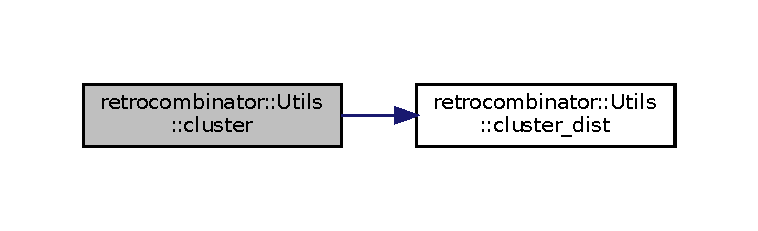
\includegraphics[width=336pt]{namespaceretrocombinator_1_1Utils_a03dcc302a7444a0c0897ea1b306e69ef_cgraph}
\end{center}
\end{figure}
Here is the caller graph for this function\+:
\nopagebreak
\begin{figure}[H]
\begin{center}
\leavevmode
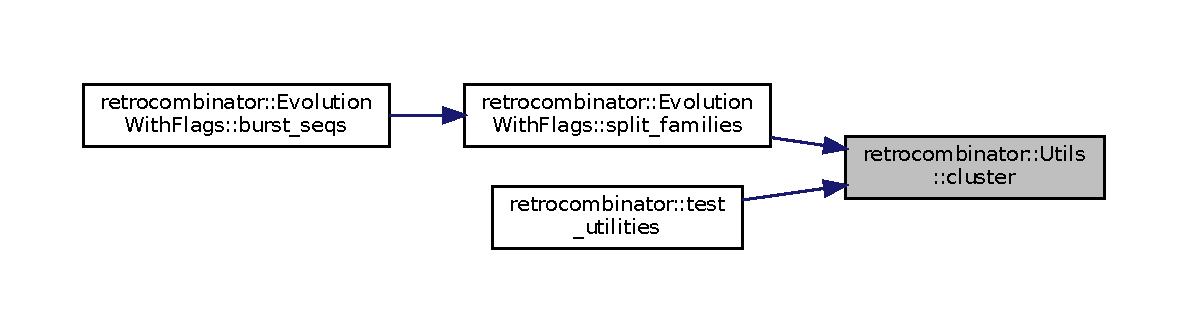
\includegraphics[width=350pt]{namespaceretrocombinator_1_1Utils_a03dcc302a7444a0c0897ea1b306e69ef_icgraph}
\end{center}
\end{figure}
\mbox{\Hypertarget{namespaceretrocombinator_1_1Utils_a75c34419887242476ac8219dfb981459}\label{namespaceretrocombinator_1_1Utils_a75c34419887242476ac8219dfb981459}} 
\index{retrocombinator\+::\+Utils@{retrocombinator\+::\+Utils}!cluster\+\_\+dist@{cluster\+\_\+dist}}
\index{cluster\+\_\+dist@{cluster\+\_\+dist}!retrocombinator\+::\+Utils@{retrocombinator\+::\+Utils}}
\subsubsection{\texorpdfstring{cluster\+\_\+dist()}{cluster\_dist()}}
{\footnotesize\ttfamily double retrocombinator\+::\+Utils\+::cluster\+\_\+dist (\begin{DoxyParamCaption}\item[{const \hyperlink{constants_8h_aa416b6a3a9e444eae3309a16b8607750}{dist\+\_\+type} \&}]{dist,  }\item[{\hyperlink{constants_8h_a8e1541b50cee66a791df4c437ccbb385}{size\+\_\+type}}]{n,  }\item[{const \hyperlink{constants_8h_a316667a6633d664fe892bd7e0eb0141e}{cluster\+\_\+type} \&}]{C1,  }\item[{const \hyperlink{constants_8h_a316667a6633d664fe892bd7e0eb0141e}{cluster\+\_\+type} \&}]{C2 }\end{DoxyParamCaption})}



Computes the cluster distance between two clusters. 

Equal to the average of all pairs (a1, a2) in C1 X C2. Here is the caller graph for this function\+:
\nopagebreak
\begin{figure}[H]
\begin{center}
\leavevmode
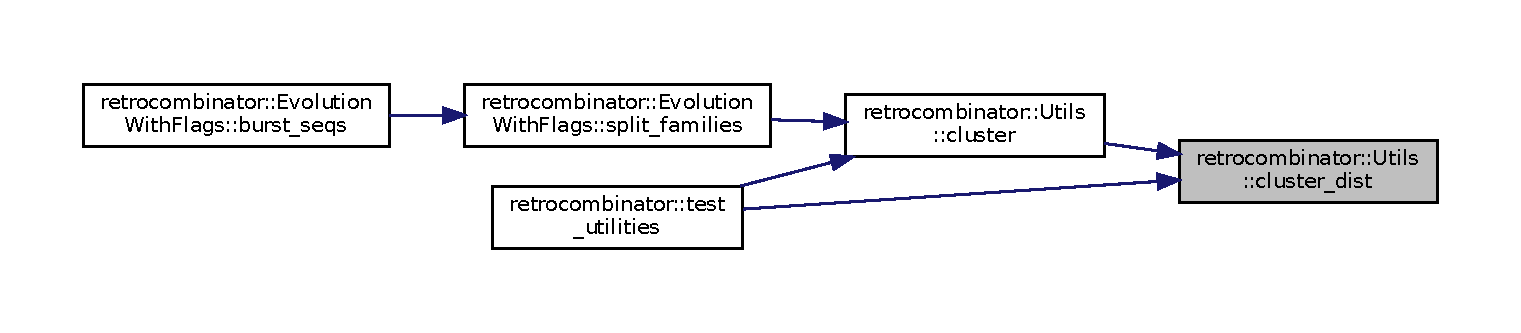
\includegraphics[width=350pt]{namespaceretrocombinator_1_1Utils_a75c34419887242476ac8219dfb981459_icgraph}
\end{center}
\end{figure}
\mbox{\Hypertarget{namespaceretrocombinator_1_1Utils_a984680ddd6d1f7ccee9e0f040ff16183}\label{namespaceretrocombinator_1_1Utils_a984680ddd6d1f7ccee9e0f040ff16183}} 
\index{retrocombinator\+::\+Utils@{retrocombinator\+::\+Utils}!is\+\_\+in\+\_\+range@{is\+\_\+in\+\_\+range}}
\index{is\+\_\+in\+\_\+range@{is\+\_\+in\+\_\+range}!retrocombinator\+::\+Utils@{retrocombinator\+::\+Utils}}
\subsubsection{\texorpdfstring{is\+\_\+in\+\_\+range()}{is\_in\_range()}}
{\footnotesize\ttfamily bool retrocombinator\+::\+Utils\+::is\+\_\+in\+\_\+range (\begin{DoxyParamCaption}\item[{\hyperlink{constants_8h_a8e1541b50cee66a791df4c437ccbb385}{size\+\_\+type}}]{test,  }\item[{\hyperlink{constants_8h_a8e1541b50cee66a791df4c437ccbb385}{size\+\_\+type}}]{lb,  }\item[{\hyperlink{constants_8h_a8e1541b50cee66a791df4c437ccbb385}{size\+\_\+type}}]{ub }\end{DoxyParamCaption})\hspace{0.3cm}{\ttfamily [inline]}}



Checks whether a number lies within a range. 

The bounds are \mbox{[}inclusive, exclusive). Here is the call graph for this function\+:
\nopagebreak
\begin{figure}[H]
\begin{center}
\leavevmode
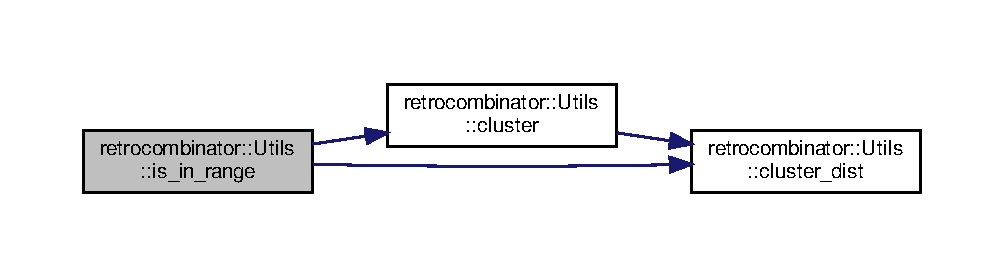
\includegraphics[width=350pt]{namespaceretrocombinator_1_1Utils_a984680ddd6d1f7ccee9e0f040ff16183_cgraph}
\end{center}
\end{figure}
Here is the caller graph for this function\+:
\nopagebreak
\begin{figure}[H]
\begin{center}
\leavevmode
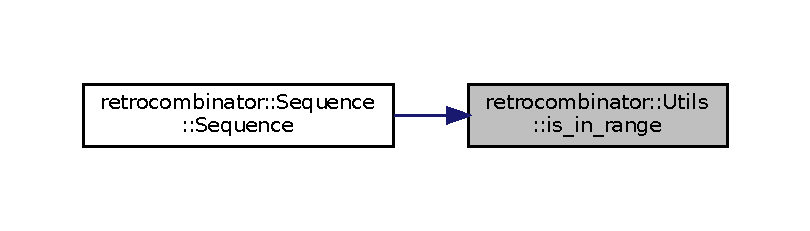
\includegraphics[width=350pt]{namespaceretrocombinator_1_1Utils_a984680ddd6d1f7ccee9e0f040ff16183_icgraph}
\end{center}
\end{figure}

\chapter{Class Documentation}
\hypertarget{classretrocombinator_1_1Evolution}{}\section{retrocombinator\+:\+:Evolution Class Reference}
\label{classretrocombinator_1_1Evolution}\index{retrocombinator\+::\+Evolution@{retrocombinator\+::\+Evolution}}


An interface for simulating the evolution of sequences.  




{\ttfamily \#include $<$evolution.\+h$>$}



Inheritance diagram for retrocombinator\+:\+:Evolution\+:
\nopagebreak
\begin{figure}[H]
\begin{center}
\leavevmode
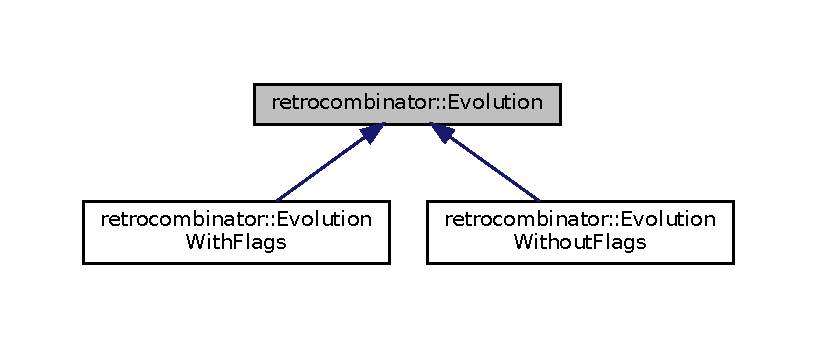
\includegraphics[width=350pt]{classretrocombinator_1_1Evolution__inherit__graph}
\end{center}
\end{figure}
\subsection*{Public Types}
\begin{DoxyCompactItemize}
\item 
\mbox{\Hypertarget{classretrocombinator_1_1Evolution_a3a0a2c09c39e368fe321fbf2e6b8af8d}\label{classretrocombinator_1_1Evolution_a3a0a2c09c39e368fe321fbf2e6b8af8d}} 
typedef \hyperlink{classretrocombinator_1_1Family_a994b8646d1c0c4e19420d2e5c6c53c85}{Family\+::seqs\+\_\+type} \hyperlink{classretrocombinator_1_1Evolution_a3a0a2c09c39e368fe321fbf2e6b8af8d}{seqs\+\_\+type}
\begin{DoxyCompactList}\small\item\em Borrow typedef from family. \end{DoxyCompactList}\end{DoxyCompactItemize}
\subsection*{Public Member Functions}
\begin{DoxyCompactItemize}
\item 
\hyperlink{classretrocombinator_1_1Evolution_a0aa94cf8dd5f6184535faf82842337fd}{Evolution} (\hyperlink{constants_8h_a8e1541b50cee66a791df4c437ccbb385}{size\+\_\+type} \hyperlink{classretrocombinator_1_1Evolution_a043c016f93a961d0e3a2fc9d257b01d9}{num\+\_\+jumps}, double \hyperlink{classretrocombinator_1_1Evolution_afdb375b975d48d9915c6e8337c33a175}{timestep}, double \hyperlink{classretrocombinator_1_1Evolution_afb663b25070c1ca619e682cef2a32196}{burst\+\_\+probability}, double \hyperlink{classretrocombinator_1_1Evolution_ac2f4821269c08b23f21b5333f2067e5f}{burst\+\_\+mean}, \hyperlink{constants_8h_a8e1541b50cee66a791df4c437ccbb385}{size\+\_\+type} \hyperlink{classretrocombinator_1_1Evolution_a0e6b2c75bdc36f8f482162f2f8c67d56}{max\+\_\+active\+\_\+copies})
\begin{DoxyCompactList}\small\item\em Set up a simulation with given parameters. \end{DoxyCompactList}\item 
virtual void \hyperlink{classretrocombinator_1_1Evolution_a0b8a181242ea8ee3072258fa7ed416f4}{evolve} (\hyperlink{classretrocombinator_1_1Output}{Output} \&output, \hyperlink{classretrocombinator_1_1PointMutator}{Point\+Mutator} \&pm, const std\+::vector$<$ std\+::string $>$ \&init\+\_\+seqs, double recomb\+\_\+mean)
\begin{DoxyCompactList}\small\item\em Run a simulation, modify the sequences, and output results to file. \end{DoxyCompactList}\item 
\mbox{\Hypertarget{classretrocombinator_1_1Evolution_a6162b87324d550c4e4e9315a640a7259}\label{classretrocombinator_1_1Evolution_a6162b87324d550c4e4e9315a640a7259}} 
virtual \hyperlink{classretrocombinator_1_1Evolution_a6162b87324d550c4e4e9315a640a7259}{$\sim$\+Evolution} ()=default
\begin{DoxyCompactList}\small\item\em Use a virtual destructor so objects can be instantiated. \end{DoxyCompactList}\end{DoxyCompactItemize}
\subsection*{Protected Member Functions}
\begin{DoxyCompactItemize}
\item 
virtual void \hyperlink{classretrocombinator_1_1Evolution_abab94a3f14460300a6a3b7a0286236a6}{burst\+\_\+seqs} (const \hyperlink{constants_8h_a8e1541b50cee66a791df4c437ccbb385}{size\+\_\+type} t, const double recomb\+\_\+mean)=0
\begin{DoxyCompactList}\small\item\em How the sequences burst after a timestep in the simulation. \end{DoxyCompactList}\end{DoxyCompactItemize}
\subsection*{Protected Attributes}
\begin{DoxyCompactItemize}
\item 
\mbox{\Hypertarget{classretrocombinator_1_1Evolution_a043c016f93a961d0e3a2fc9d257b01d9}\label{classretrocombinator_1_1Evolution_a043c016f93a961d0e3a2fc9d257b01d9}} 
const \hyperlink{constants_8h_a8e1541b50cee66a791df4c437ccbb385}{size\+\_\+type} \hyperlink{classretrocombinator_1_1Evolution_a043c016f93a961d0e3a2fc9d257b01d9}{num\+\_\+jumps}
\begin{DoxyCompactList}\small\item\em Number of jumps in our simulation. \end{DoxyCompactList}\item 
\mbox{\Hypertarget{classretrocombinator_1_1Evolution_afdb375b975d48d9915c6e8337c33a175}\label{classretrocombinator_1_1Evolution_afdb375b975d48d9915c6e8337c33a175}} 
const double \hyperlink{classretrocombinator_1_1Evolution_afdb375b975d48d9915c6e8337c33a175}{timestep}
\begin{DoxyCompactList}\small\item\em How much time has passed in one jump (in millions of years) \end{DoxyCompactList}\item 
\mbox{\Hypertarget{classretrocombinator_1_1Evolution_afb663b25070c1ca619e682cef2a32196}\label{classretrocombinator_1_1Evolution_afb663b25070c1ca619e682cef2a32196}} 
const double \hyperlink{classretrocombinator_1_1Evolution_afb663b25070c1ca619e682cef2a32196}{burst\+\_\+probability}
\begin{DoxyCompactList}\small\item\em Probability that an active sequence bursts in {\itshape timestep}. \end{DoxyCompactList}\item 
\mbox{\Hypertarget{classretrocombinator_1_1Evolution_ac2f4821269c08b23f21b5333f2067e5f}\label{classretrocombinator_1_1Evolution_ac2f4821269c08b23f21b5333f2067e5f}} 
const double \hyperlink{classretrocombinator_1_1Evolution_ac2f4821269c08b23f21b5333f2067e5f}{burst\+\_\+mean}
\begin{DoxyCompactList}\small\item\em The Poisson mean for new number of sequences to be created. \end{DoxyCompactList}\item 
\mbox{\Hypertarget{classretrocombinator_1_1Evolution_a0e6b2c75bdc36f8f482162f2f8c67d56}\label{classretrocombinator_1_1Evolution_a0e6b2c75bdc36f8f482162f2f8c67d56}} 
const \hyperlink{constants_8h_a8e1541b50cee66a791df4c437ccbb385}{size\+\_\+type} \hyperlink{classretrocombinator_1_1Evolution_a0e6b2c75bdc36f8f482162f2f8c67d56}{max\+\_\+active\+\_\+copies}
\begin{DoxyCompactList}\small\item\em The total number of sequences that have the ability to burst we allow in our simulation. \end{DoxyCompactList}\item 
std\+::list$<$ \hyperlink{classretrocombinator_1_1Family}{Family} $>$ \hyperlink{classretrocombinator_1_1Evolution_a163715452c511724ecc0ef16a5030dea}{families}
\begin{DoxyCompactList}\small\item\em The actual values of the sequences during the simulation. \end{DoxyCompactList}\item 
\mbox{\Hypertarget{classretrocombinator_1_1Evolution_abc218e27bae28eb73089e56cc8b51b4e}\label{classretrocombinator_1_1Evolution_abc218e27bae28eb73089e56cc8b51b4e}} 
\hyperlink{constants_8h_a8e1541b50cee66a791df4c437ccbb385}{size\+\_\+type} \hyperlink{classretrocombinator_1_1Evolution_abc218e27bae28eb73089e56cc8b51b4e}{total\+\_\+num\+\_\+sequences}
\begin{DoxyCompactList}\small\item\em The overall number of sequences across all families. \end{DoxyCompactList}\end{DoxyCompactItemize}


\subsection{Detailed Description}
An interface for simulating the evolution of sequences. 

Provides basic functionality, all subclasses specialise some methods provided by this class to add events/flags/copy trees etc. 

\subsection{Constructor \& Destructor Documentation}
\mbox{\Hypertarget{classretrocombinator_1_1Evolution_a0aa94cf8dd5f6184535faf82842337fd}\label{classretrocombinator_1_1Evolution_a0aa94cf8dd5f6184535faf82842337fd}} 
\index{retrocombinator\+::\+Evolution@{retrocombinator\+::\+Evolution}!Evolution@{Evolution}}
\index{Evolution@{Evolution}!retrocombinator\+::\+Evolution@{retrocombinator\+::\+Evolution}}
\subsubsection{\texorpdfstring{Evolution()}{Evolution()}}
{\footnotesize\ttfamily Evolution\+::\+Evolution (\begin{DoxyParamCaption}\item[{\hyperlink{constants_8h_a8e1541b50cee66a791df4c437ccbb385}{size\+\_\+type}}]{num\+\_\+jumps,  }\item[{double}]{timestep,  }\item[{double}]{burst\+\_\+probability,  }\item[{double}]{burst\+\_\+mean,  }\item[{\hyperlink{constants_8h_a8e1541b50cee66a791df4c437ccbb385}{size\+\_\+type}}]{max\+\_\+active\+\_\+copies }\end{DoxyParamCaption})}



Set up a simulation with given parameters. 

Look at documenation for the individual members to understand what they mean. 

\subsection{Member Function Documentation}
\mbox{\Hypertarget{classretrocombinator_1_1Evolution_abab94a3f14460300a6a3b7a0286236a6}\label{classretrocombinator_1_1Evolution_abab94a3f14460300a6a3b7a0286236a6}} 
\index{retrocombinator\+::\+Evolution@{retrocombinator\+::\+Evolution}!burst\+\_\+seqs@{burst\+\_\+seqs}}
\index{burst\+\_\+seqs@{burst\+\_\+seqs}!retrocombinator\+::\+Evolution@{retrocombinator\+::\+Evolution}}
\subsubsection{\texorpdfstring{burst\+\_\+seqs()}{burst\_seqs()}}
{\footnotesize\ttfamily virtual void retrocombinator\+::\+Evolution\+::burst\+\_\+seqs (\begin{DoxyParamCaption}\item[{const \hyperlink{constants_8h_a8e1541b50cee66a791df4c437ccbb385}{size\+\_\+type}}]{t,  }\item[{const double}]{recomb\+\_\+mean }\end{DoxyParamCaption})\hspace{0.3cm}{\ttfamily [protected]}, {\ttfamily [pure virtual]}}



How the sequences burst after a timestep in the simulation. 

To be implemented by a derived class, depending on our assumptions. 

Implemented in \hyperlink{classretrocombinator_1_1EvolutionWithoutFlags_aeba3cc75049e0590e5dcaab9558f8c56}{retrocombinator\+::\+Evolution\+Without\+Flags}, and \hyperlink{classretrocombinator_1_1EvolutionWithFlags_abad180fa8494b259e5167a13285347dd}{retrocombinator\+::\+Evolution\+With\+Flags}.

Here is the caller graph for this function\+:
\nopagebreak
\begin{figure}[H]
\begin{center}
\leavevmode
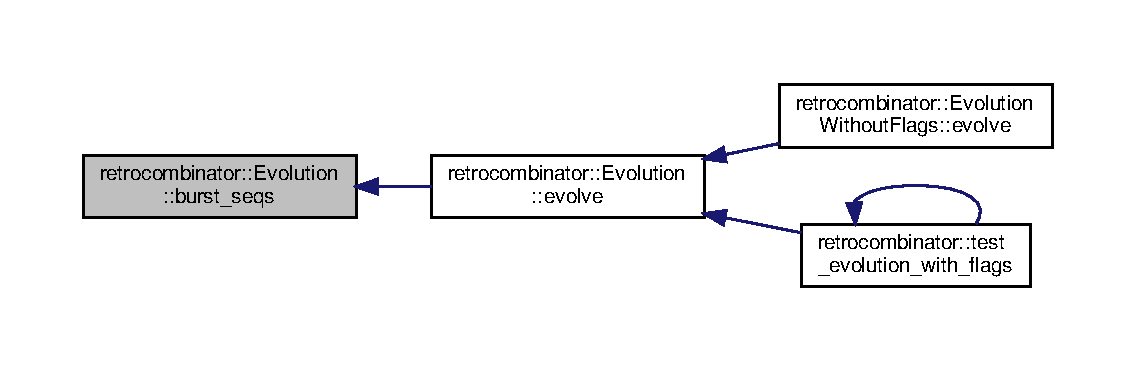
\includegraphics[width=350pt]{classretrocombinator_1_1Evolution_abab94a3f14460300a6a3b7a0286236a6_icgraph}
\end{center}
\end{figure}
\mbox{\Hypertarget{classretrocombinator_1_1Evolution_a0b8a181242ea8ee3072258fa7ed416f4}\label{classretrocombinator_1_1Evolution_a0b8a181242ea8ee3072258fa7ed416f4}} 
\index{retrocombinator\+::\+Evolution@{retrocombinator\+::\+Evolution}!evolve@{evolve}}
\index{evolve@{evolve}!retrocombinator\+::\+Evolution@{retrocombinator\+::\+Evolution}}
\subsubsection{\texorpdfstring{evolve()}{evolve()}}
{\footnotesize\ttfamily void Evolution\+::evolve (\begin{DoxyParamCaption}\item[{\hyperlink{classretrocombinator_1_1Output}{Output} \&}]{output,  }\item[{\hyperlink{classretrocombinator_1_1PointMutator}{Point\+Mutator} \&}]{pm,  }\item[{const std\+::vector$<$ std\+::string $>$ \&}]{init\+\_\+seqs,  }\item[{double}]{recomb\+\_\+mean }\end{DoxyParamCaption})\hspace{0.3cm}{\ttfamily [virtual]}}



Run a simulation, modify the sequences, and output results to file. 

output\+: where we write to disc pm\+: the point mutator we use in our simulation init\+\_\+seqs\+: the initial sequences we start with recomb\+\_\+mean\+: the expected number of template switches 

Reimplemented in \hyperlink{classretrocombinator_1_1EvolutionWithoutFlags_a9e27b532826998a88d2c157daf53c447}{retrocombinator\+::\+Evolution\+Without\+Flags}.

Here is the call graph for this function\+:
\nopagebreak
\begin{figure}[H]
\begin{center}
\leavevmode
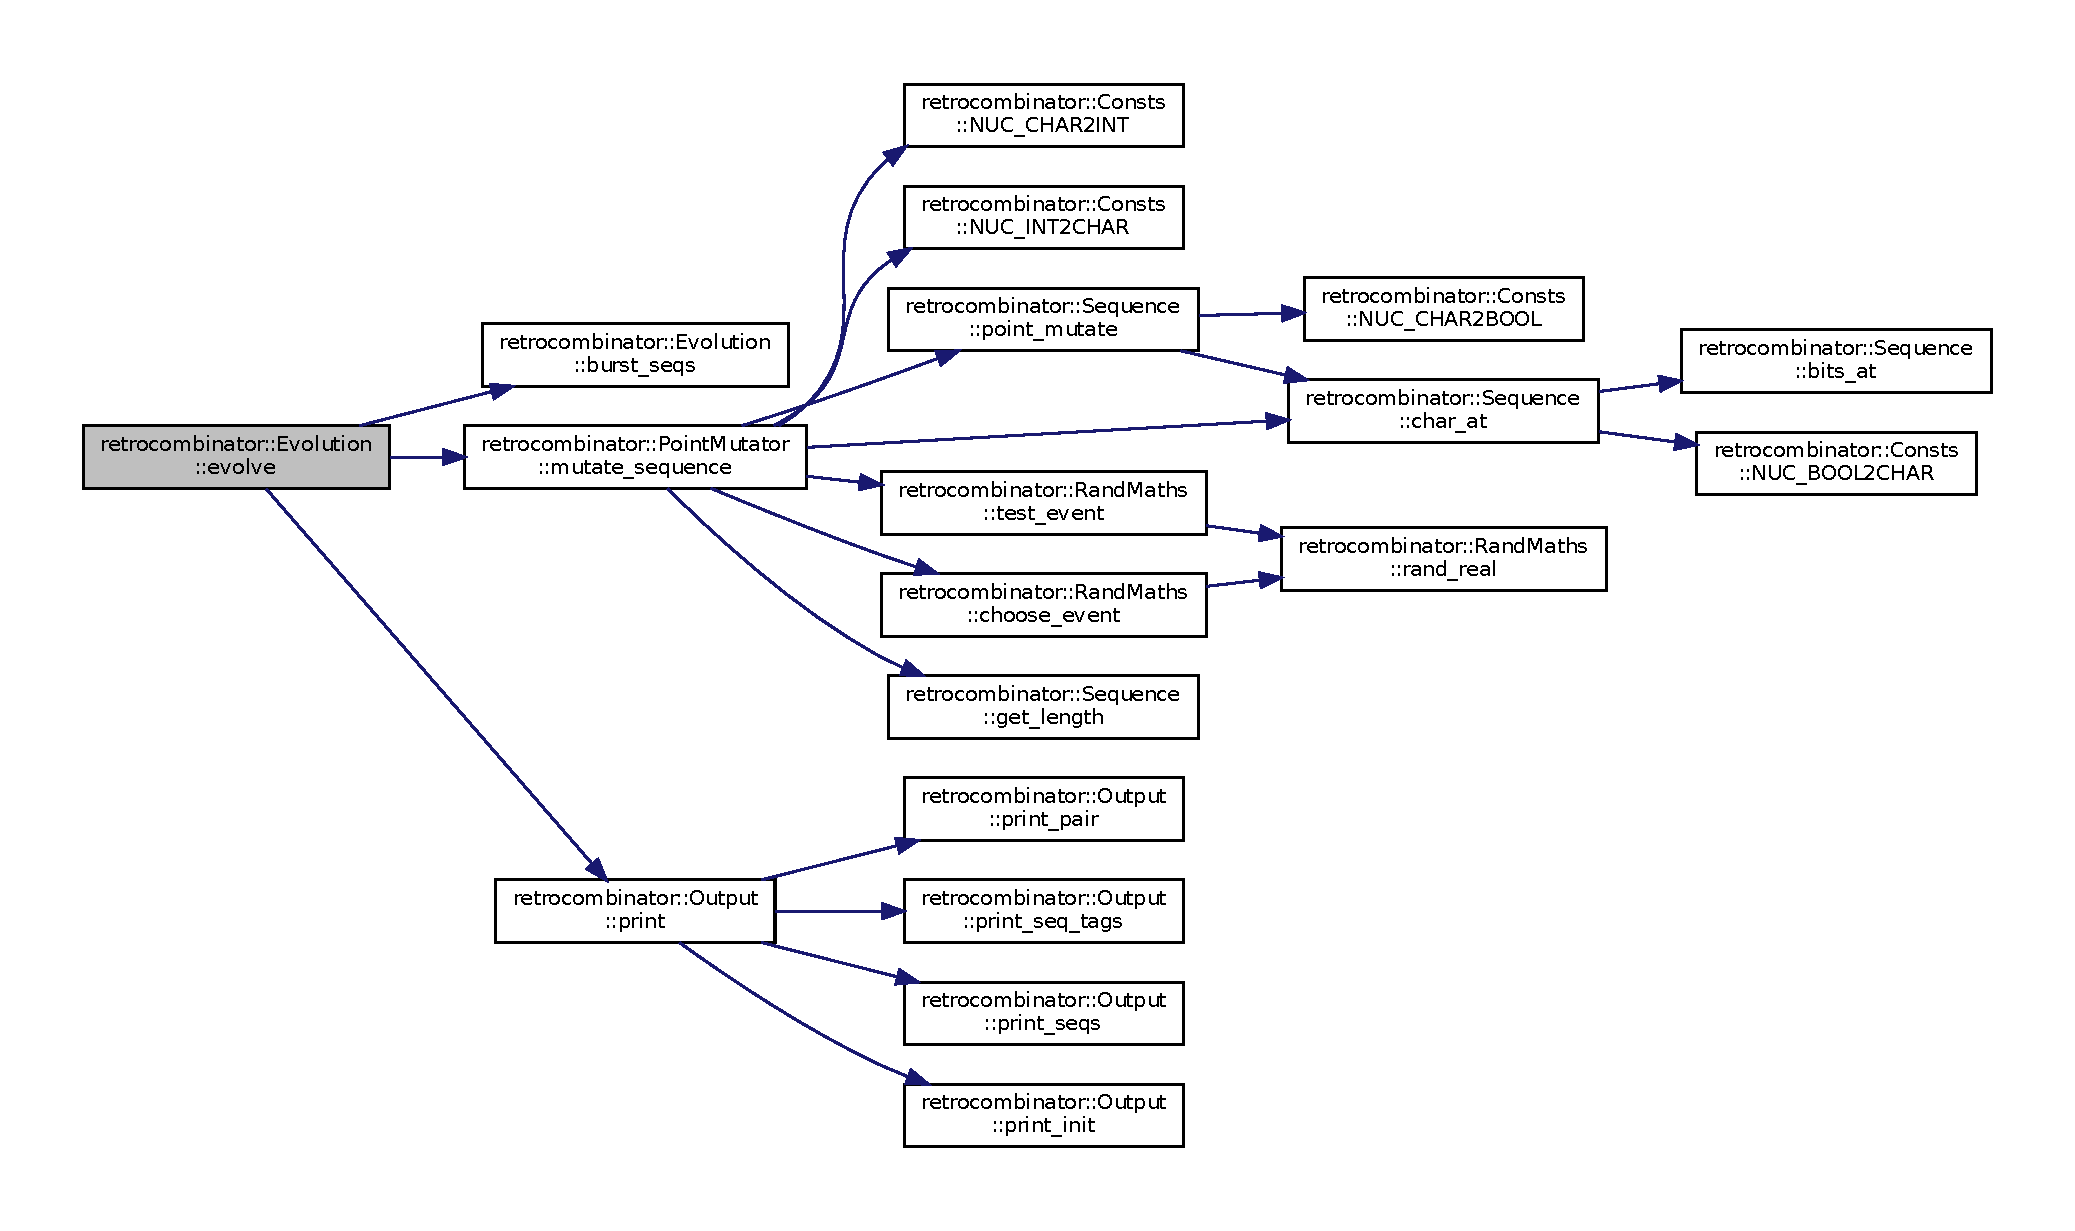
\includegraphics[width=350pt]{classretrocombinator_1_1Evolution_a0b8a181242ea8ee3072258fa7ed416f4_cgraph}
\end{center}
\end{figure}
Here is the caller graph for this function\+:
\nopagebreak
\begin{figure}[H]
\begin{center}
\leavevmode
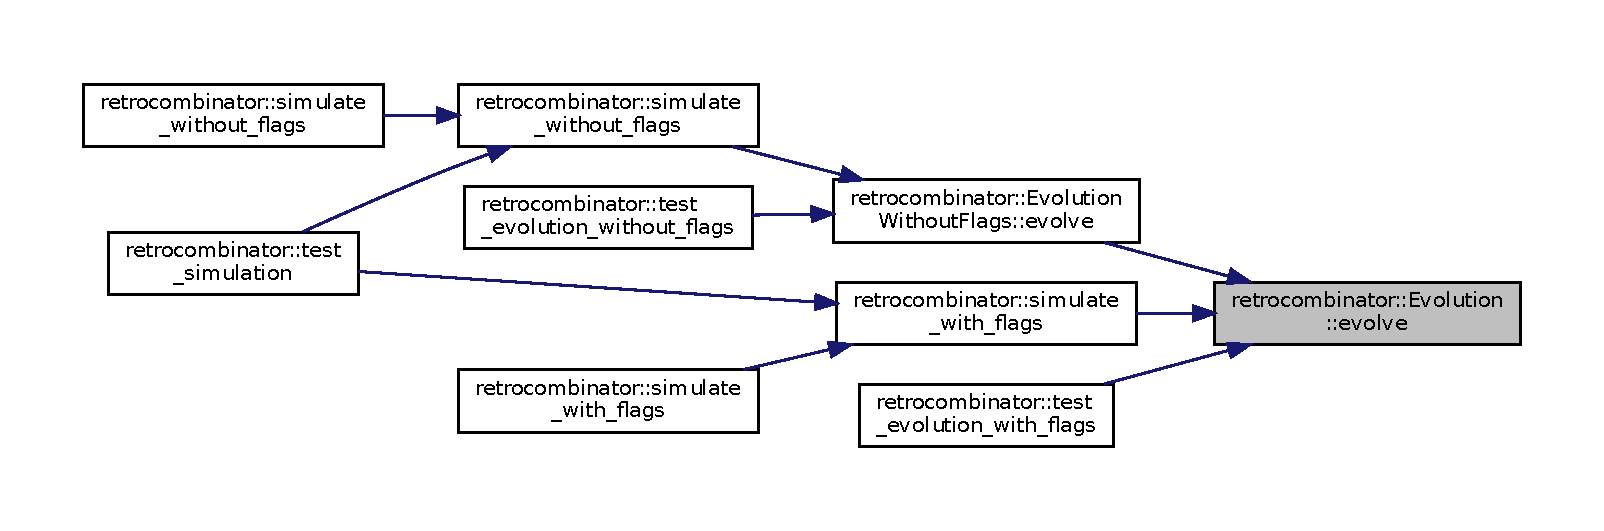
\includegraphics[width=350pt]{classretrocombinator_1_1Evolution_a0b8a181242ea8ee3072258fa7ed416f4_icgraph}
\end{center}
\end{figure}


\subsection{Member Data Documentation}
\mbox{\Hypertarget{classretrocombinator_1_1Evolution_a163715452c511724ecc0ef16a5030dea}\label{classretrocombinator_1_1Evolution_a163715452c511724ecc0ef16a5030dea}} 
\index{retrocombinator\+::\+Evolution@{retrocombinator\+::\+Evolution}!families@{families}}
\index{families@{families}!retrocombinator\+::\+Evolution@{retrocombinator\+::\+Evolution}}
\subsubsection{\texorpdfstring{families}{families}}
{\footnotesize\ttfamily std\+::list$<$\hyperlink{classretrocombinator_1_1Family}{Family}$>$ retrocombinator\+::\+Evolution\+::families\hspace{0.3cm}{\ttfamily [protected]}}



The actual values of the sequences during the simulation. 

All sequences in family {\itshape i} are present in families\mbox{[}i\mbox{]}. N\+O\+TE\+: Needs to be list so that iterators are valid after insertion/deletion of families. 

The documentation for this class was generated from the following files\+:\begin{DoxyCompactItemize}
\item 
src/evolution.\+h\item 
src/evolution.\+cpp\end{DoxyCompactItemize}

\hypertarget{classretrocombinator_1_1EvolutionWithFlags}{}\section{retrocombinator\+:\+:Evolution\+With\+Flags Class Reference}
\label{classretrocombinator_1_1EvolutionWithFlags}\index{retrocombinator\+::\+Evolution\+With\+Flags@{retrocombinator\+::\+Evolution\+With\+Flags}}


A simulation where some sequences can become inactive over time.  




{\ttfamily \#include $<$evolution\+\_\+with\+\_\+flags.\+h$>$}



Inheritance diagram for retrocombinator\+:\+:Evolution\+With\+Flags\+:\nopagebreak
\begin{figure}[H]
\begin{center}
\leavevmode
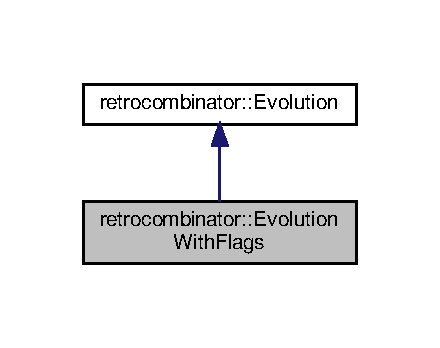
\includegraphics[width=211pt]{classretrocombinator_1_1EvolutionWithFlags__inherit__graph}
\end{center}
\end{figure}


Collaboration diagram for retrocombinator\+:\+:Evolution\+With\+Flags\+:\nopagebreak
\begin{figure}[H]
\begin{center}
\leavevmode
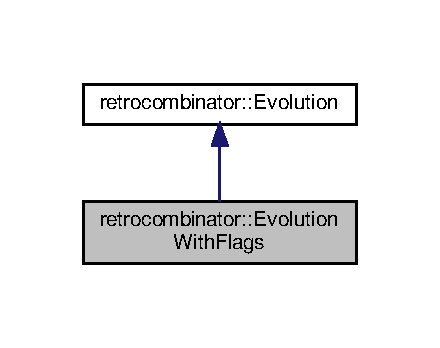
\includegraphics[width=211pt]{classretrocombinator_1_1EvolutionWithFlags__coll__graph}
\end{center}
\end{figure}
\subsection*{Public Member Functions}
\begin{DoxyCompactItemize}
\item 
\hyperlink{classretrocombinator_1_1EvolutionWithFlags_a4e7809583d5dcf9cf9c1155587d7e99e}{Evolution\+With\+Flags} (\hyperlink{namespaceretrocombinator_a8e1541b50cee66a791df4c437ccbb385}{size\+\_\+type} \hyperlink{classretrocombinator_1_1Evolution_a043c016f93a961d0e3a2fc9d257b01d9}{num\+\_\+jumps}, double \hyperlink{classretrocombinator_1_1Evolution_afdb375b975d48d9915c6e8337c33a175}{timestep}, double \hyperlink{classretrocombinator_1_1Evolution_afb663b25070c1ca619e682cef2a32196}{burst\+\_\+probability}, double \hyperlink{classretrocombinator_1_1Evolution_ac2f4821269c08b23f21b5333f2067e5f}{burst\+\_\+mean}, \hyperlink{namespaceretrocombinator_a8e1541b50cee66a791df4c437ccbb385}{size\+\_\+type} \hyperlink{classretrocombinator_1_1Evolution_a0e6b2c75bdc36f8f482162f2f8c67d56}{max\+\_\+active\+\_\+copies}, \hyperlink{namespaceretrocombinator_a8e1541b50cee66a791df4c437ccbb385}{size\+\_\+type} \hyperlink{classretrocombinator_1_1EvolutionWithFlags_a8fa5c08653bfdf6425ac1dc4a0100642}{max\+\_\+total\+\_\+copies})
\begin{DoxyCompactList}\small\item\em Inherited constructor. \end{DoxyCompactList}\item 
\mbox{\Hypertarget{classretrocombinator_1_1EvolutionWithFlags_a3dd922a0ddfa93218e95f733332c21f3}\label{classretrocombinator_1_1EvolutionWithFlags_a3dd922a0ddfa93218e95f733332c21f3}} 
void \hyperlink{classretrocombinator_1_1EvolutionWithFlags_a3dd922a0ddfa93218e95f733332c21f3}{set\+\_\+selection\+\_\+threshold} (double percentage)
\begin{DoxyCompactList}\small\item\em To kill sequences that have diverged too much. \end{DoxyCompactList}\item 
void \hyperlink{classretrocombinator_1_1EvolutionWithFlags_ad94cabcb6a894d503c3d84c6022a1438}{use\+\_\+families\+\_\+at} (double proportion, double percentage)
\begin{DoxyCompactList}\small\item\em To prevent distant sequences from recombining. \end{DoxyCompactList}\end{DoxyCompactItemize}
\subsection*{Protected Member Functions}
\begin{DoxyCompactItemize}
\item 
\mbox{\Hypertarget{classretrocombinator_1_1EvolutionWithFlags_abad180fa8494b259e5167a13285347dd}\label{classretrocombinator_1_1EvolutionWithFlags_abad180fa8494b259e5167a13285347dd}} 
void \hyperlink{classretrocombinator_1_1EvolutionWithFlags_abad180fa8494b259e5167a13285347dd}{burst\+\_\+seqs} (const \hyperlink{namespaceretrocombinator_a8e1541b50cee66a791df4c437ccbb385}{size\+\_\+type} t, const double recomb\+\_\+mean) override
\begin{DoxyCompactList}\small\item\em Burst by taking into consideration activity of sequences, events, and selection. \end{DoxyCompactList}\item 
void \hyperlink{classretrocombinator_1_1EvolutionWithFlags_ae5a9e278233d2ea42bdef4df66d4b5b9}{kill\+\_\+sequences} (\hyperlink{namespaceretrocombinator_a8e1541b50cee66a791df4c437ccbb385}{size\+\_\+type} num\+\_\+active\+\_\+copies, \hyperlink{namespaceretrocombinator_a8e1541b50cee66a791df4c437ccbb385}{size\+\_\+type} num\+\_\+total\+\_\+copies)
\begin{DoxyCompactList}\small\item\em Kill excess sequences. \end{DoxyCompactList}\item 
\mbox{\Hypertarget{classretrocombinator_1_1EvolutionWithFlags_adbf96b693339f0b902ba1a2bb83a01d4}\label{classretrocombinator_1_1EvolutionWithFlags_adbf96b693339f0b902ba1a2bb83a01d4}} 
void \hyperlink{classretrocombinator_1_1EvolutionWithFlags_adbf96b693339f0b902ba1a2bb83a01d4}{remove\+\_\+dead\+\_\+families} ()
\begin{DoxyCompactList}\small\item\em Removes empty families. \end{DoxyCompactList}\item 
\mbox{\Hypertarget{classretrocombinator_1_1EvolutionWithFlags_a53b7da04d209f7c1adb2f74af5d56149}\label{classretrocombinator_1_1EvolutionWithFlags_a53b7da04d209f7c1adb2f74af5d56149}} 
void \hyperlink{classretrocombinator_1_1EvolutionWithFlags_a53b7da04d209f7c1adb2f74af5d56149}{split\+\_\+families} ()
\begin{DoxyCompactList}\small\item\em To split any large family into two families that can no longer recombine with each other. \end{DoxyCompactList}\end{DoxyCompactItemize}
\subsection*{Protected Attributes}
\begin{DoxyCompactItemize}
\item 
\mbox{\Hypertarget{classretrocombinator_1_1EvolutionWithFlags_a8fa5c08653bfdf6425ac1dc4a0100642}\label{classretrocombinator_1_1EvolutionWithFlags_a8fa5c08653bfdf6425ac1dc4a0100642}} 
const \hyperlink{namespaceretrocombinator_a8e1541b50cee66a791df4c437ccbb385}{size\+\_\+type} \hyperlink{classretrocombinator_1_1EvolutionWithFlags_a8fa5c08653bfdf6425ac1dc4a0100642}{max\+\_\+total\+\_\+copies}
\begin{DoxyCompactList}\small\item\em The total number of sequences (active + inactive) we allow in our simulation. \end{DoxyCompactList}\item 
\mbox{\Hypertarget{classretrocombinator_1_1EvolutionWithFlags_ad05bfc6282a746b9b67a1591f0a0073b}\label{classretrocombinator_1_1EvolutionWithFlags_ad05bfc6282a746b9b67a1591f0a0073b}} 
double \hyperlink{classretrocombinator_1_1EvolutionWithFlags_ad05bfc6282a746b9b67a1591f0a0073b}{selection\+\_\+threshold}
\begin{DoxyCompactList}\small\item\em What percentage sequence similarity to the original we wish to maintain. \end{DoxyCompactList}\end{DoxyCompactItemize}
\textbf{ }\par
\begin{DoxyCompactItemize}
\item 
double \hyperlink{classretrocombinator_1_1EvolutionWithFlags_a6bd3b124459c847b387b5d083abf0a98}{fam\+\_\+proportion}
\begin{DoxyCompactList}\small\item\em Parameters for deciding when to split a family into two. \end{DoxyCompactList}\item 
\mbox{\Hypertarget{classretrocombinator_1_1EvolutionWithFlags_ab731b0628b1a9bebb61cd3f86e9321ea}\label{classretrocombinator_1_1EvolutionWithFlags_ab731b0628b1a9bebb61cd3f86e9321ea}} 
double {\bfseries fam\+\_\+percentage}
\end{DoxyCompactItemize}

\subsection*{Additional Inherited Members}


\subsection{Detailed Description}
A simulation where some sequences can become inactive over time. 

A sequence becomes inactive if some sensitive positions are mutated. The sequence is then \textquotesingle{}flagged\textquotesingle{}. 

\subsection{Constructor \& Destructor Documentation}
\mbox{\Hypertarget{classretrocombinator_1_1EvolutionWithFlags_a4e7809583d5dcf9cf9c1155587d7e99e}\label{classretrocombinator_1_1EvolutionWithFlags_a4e7809583d5dcf9cf9c1155587d7e99e}} 
\index{retrocombinator\+::\+Evolution\+With\+Flags@{retrocombinator\+::\+Evolution\+With\+Flags}!Evolution\+With\+Flags@{Evolution\+With\+Flags}}
\index{Evolution\+With\+Flags@{Evolution\+With\+Flags}!retrocombinator\+::\+Evolution\+With\+Flags@{retrocombinator\+::\+Evolution\+With\+Flags}}
\subsubsection{\texorpdfstring{Evolution\+With\+Flags()}{EvolutionWithFlags()}}
{\footnotesize\ttfamily Evolution\+With\+Flags\+::\+Evolution\+With\+Flags (\begin{DoxyParamCaption}\item[{\hyperlink{namespaceretrocombinator_a8e1541b50cee66a791df4c437ccbb385}{size\+\_\+type}}]{num\+\_\+jumps,  }\item[{double}]{timestep,  }\item[{double}]{burst\+\_\+probability,  }\item[{double}]{burst\+\_\+mean,  }\item[{\hyperlink{namespaceretrocombinator_a8e1541b50cee66a791df4c437ccbb385}{size\+\_\+type}}]{max\+\_\+active\+\_\+copies,  }\item[{\hyperlink{namespaceretrocombinator_a8e1541b50cee66a791df4c437ccbb385}{size\+\_\+type}}]{max\+\_\+total\+\_\+copies }\end{DoxyParamCaption})}



Inherited constructor. 

{\ttfamily max\+\_\+total\+\_\+copies} is the total number of active and inactive sequences that we allow in our simulation. 

\subsection{Member Function Documentation}
\mbox{\Hypertarget{classretrocombinator_1_1EvolutionWithFlags_ae5a9e278233d2ea42bdef4df66d4b5b9}\label{classretrocombinator_1_1EvolutionWithFlags_ae5a9e278233d2ea42bdef4df66d4b5b9}} 
\index{retrocombinator\+::\+Evolution\+With\+Flags@{retrocombinator\+::\+Evolution\+With\+Flags}!kill\+\_\+sequences@{kill\+\_\+sequences}}
\index{kill\+\_\+sequences@{kill\+\_\+sequences}!retrocombinator\+::\+Evolution\+With\+Flags@{retrocombinator\+::\+Evolution\+With\+Flags}}
\subsubsection{\texorpdfstring{kill\+\_\+sequences()}{kill\_sequences()}}
{\footnotesize\ttfamily void Evolution\+With\+Flags\+::kill\+\_\+sequences (\begin{DoxyParamCaption}\item[{\hyperlink{namespaceretrocombinator_a8e1541b50cee66a791df4c437ccbb385}{size\+\_\+type}}]{num\+\_\+active\+\_\+copies,  }\item[{\hyperlink{namespaceretrocombinator_a8e1541b50cee66a791df4c437ccbb385}{size\+\_\+type}}]{num\+\_\+total\+\_\+copies }\end{DoxyParamCaption})\hspace{0.3cm}{\ttfamily [protected]}}



Kill excess sequences. 

Provide the number of active sequences and total sequences currently, remove sequences until we have met both selection threshold needs and max\+\_\+copies needs. Here is the call graph for this function\+:\nopagebreak
\begin{figure}[H]
\begin{center}
\leavevmode
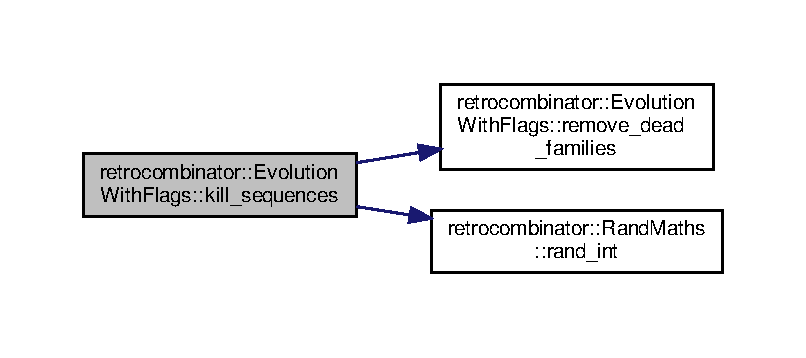
\includegraphics[width=350pt]{classretrocombinator_1_1EvolutionWithFlags_ae5a9e278233d2ea42bdef4df66d4b5b9_cgraph}
\end{center}
\end{figure}
Here is the caller graph for this function\+:\nopagebreak
\begin{figure}[H]
\begin{center}
\leavevmode
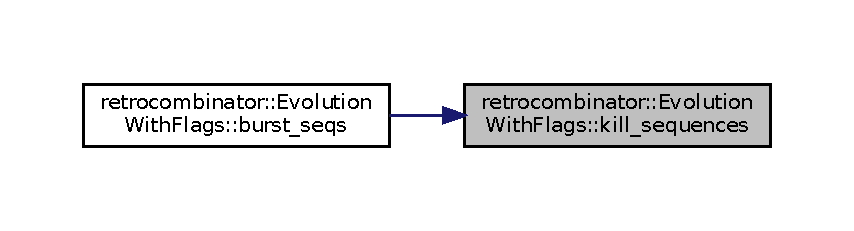
\includegraphics[width=350pt]{classretrocombinator_1_1EvolutionWithFlags_ae5a9e278233d2ea42bdef4df66d4b5b9_icgraph}
\end{center}
\end{figure}
\mbox{\Hypertarget{classretrocombinator_1_1EvolutionWithFlags_ad94cabcb6a894d503c3d84c6022a1438}\label{classretrocombinator_1_1EvolutionWithFlags_ad94cabcb6a894d503c3d84c6022a1438}} 
\index{retrocombinator\+::\+Evolution\+With\+Flags@{retrocombinator\+::\+Evolution\+With\+Flags}!use\+\_\+families\+\_\+at@{use\+\_\+families\+\_\+at}}
\index{use\+\_\+families\+\_\+at@{use\+\_\+families\+\_\+at}!retrocombinator\+::\+Evolution\+With\+Flags@{retrocombinator\+::\+Evolution\+With\+Flags}}
\subsubsection{\texorpdfstring{use\+\_\+families\+\_\+at()}{use\_families\_at()}}
{\footnotesize\ttfamily void Evolution\+With\+Flags\+::use\+\_\+families\+\_\+at (\begin{DoxyParamCaption}\item[{double}]{proportion,  }\item[{double}]{percentage }\end{DoxyParamCaption})}



To prevent distant sequences from recombining. 

If {\ttfamily proportion} of the sequence similarity matrix goes below {\ttfamily percentage} then split the family into two. Here is the caller graph for this function\+:
\nopagebreak
\begin{figure}[H]
\begin{center}
\leavevmode
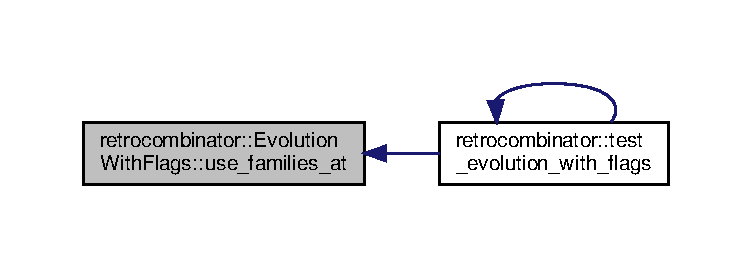
\includegraphics[width=350pt]{classretrocombinator_1_1EvolutionWithFlags_ad94cabcb6a894d503c3d84c6022a1438_icgraph}
\end{center}
\end{figure}


\subsection{Member Data Documentation}
\mbox{\Hypertarget{classretrocombinator_1_1EvolutionWithFlags_a6bd3b124459c847b387b5d083abf0a98}\label{classretrocombinator_1_1EvolutionWithFlags_a6bd3b124459c847b387b5d083abf0a98}} 
\index{retrocombinator\+::\+Evolution\+With\+Flags@{retrocombinator\+::\+Evolution\+With\+Flags}!fam\+\_\+proportion@{fam\+\_\+proportion}}
\index{fam\+\_\+proportion@{fam\+\_\+proportion}!retrocombinator\+::\+Evolution\+With\+Flags@{retrocombinator\+::\+Evolution\+With\+Flags}}
\subsubsection{\texorpdfstring{fam\+\_\+proportion}{fam\_proportion}}
{\footnotesize\ttfamily double retrocombinator\+::\+Evolution\+With\+Flags\+::fam\+\_\+proportion\hspace{0.3cm}{\ttfamily [protected]}}



Parameters for deciding when to split a family into two. 

If {\ttfamily fam\+\_\+proportion} of the sequence similarity matrix goes below {\ttfamily fam\+\_\+percentage} then split the family into two. 

The documentation for this class was generated from the following files\+:\begin{DoxyCompactItemize}
\item 
src/evolution\+\_\+with\+\_\+flags.\+h\item 
src/evolution\+\_\+with\+\_\+flags.\+cpp\end{DoxyCompactItemize}

\hypertarget{classretrocombinator_1_1EvolutionWithoutFlags}{}\section{retrocombinator\+:\+:Evolution\+Without\+Flags Class Reference}
\label{classretrocombinator_1_1EvolutionWithoutFlags}\index{retrocombinator\+::\+Evolution\+Without\+Flags@{retrocombinator\+::\+Evolution\+Without\+Flags}}


A simulation where all sequences are active.  




{\ttfamily \#include $<$evolution\+\_\+without\+\_\+flags.\+h$>$}



Inheritance diagram for retrocombinator\+:\+:Evolution\+Without\+Flags\+:\nopagebreak
\begin{figure}[H]
\begin{center}
\leavevmode
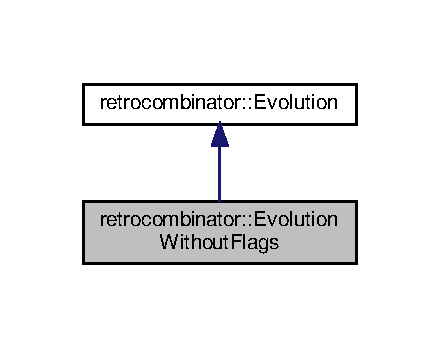
\includegraphics[width=211pt]{classretrocombinator_1_1EvolutionWithoutFlags__inherit__graph}
\end{center}
\end{figure}


Collaboration diagram for retrocombinator\+:\+:Evolution\+Without\+Flags\+:\nopagebreak
\begin{figure}[H]
\begin{center}
\leavevmode
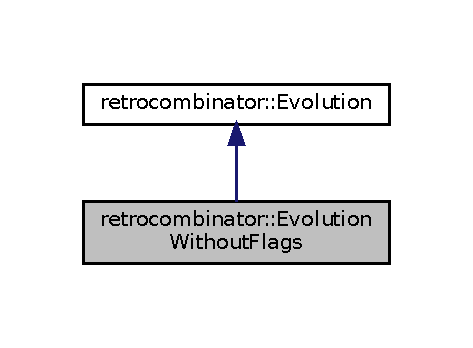
\includegraphics[width=211pt]{classretrocombinator_1_1EvolutionWithoutFlags__coll__graph}
\end{center}
\end{figure}
\subsection*{Public Types}
\begin{DoxyCompactItemize}
\item 
typedef std\+::vector$<$ std\+::list$<$ std\+::pair$<$ \hyperlink{namespaceretrocombinator_afd7c6eb4293e8c4d12827609a9a34b9b}{tag\+\_\+type}, \hyperlink{namespaceretrocombinator_afd7c6eb4293e8c4d12827609a9a34b9b}{tag\+\_\+type} $>$ $>$ $>$ \hyperlink{classretrocombinator_1_1EvolutionWithoutFlags_ac6bd9b8af2b258bf76aae5b62ef78327}{tree\+\_\+type}
\begin{DoxyCompactList}\small\item\em To represent a phyogenetic tree. \end{DoxyCompactList}\end{DoxyCompactItemize}
\subsection*{Public Member Functions}
\begin{DoxyCompactItemize}
\item 
\mbox{\Hypertarget{classretrocombinator_1_1EvolutionWithoutFlags_a4fdf9c23da86d61f99a1f51c119e3ce2}\label{classretrocombinator_1_1EvolutionWithoutFlags_a4fdf9c23da86d61f99a1f51c119e3ce2}} 
void \hyperlink{classretrocombinator_1_1EvolutionWithoutFlags_a4fdf9c23da86d61f99a1f51c119e3ce2}{calculate\+\_\+copy\+\_\+number\+\_\+tree} (\hyperlink{namespaceretrocombinator_a8e1541b50cee66a791df4c437ccbb385}{size\+\_\+type} num\+\_\+init\+\_\+seq)
\begin{DoxyCompactList}\small\item\em Calculates the copy numbers of the sequences for all times. \end{DoxyCompactList}\item 
\mbox{\Hypertarget{classretrocombinator_1_1EvolutionWithoutFlags_a9e27b532826998a88d2c157daf53c447}\label{classretrocombinator_1_1EvolutionWithoutFlags_a9e27b532826998a88d2c157daf53c447}} 
void \hyperlink{classretrocombinator_1_1EvolutionWithoutFlags_a9e27b532826998a88d2c157daf53c447}{evolve} (\hyperlink{classretrocombinator_1_1Output}{Output} \&output, \hyperlink{classretrocombinator_1_1PointMutator}{Point\+Mutator} \&pm, const std\+::vector$<$ std\+::string $>$ \&init\+\_\+seqs, double recomb\+\_\+mean) override
\begin{DoxyCompactList}\small\item\em Overrides to create a copy number tree if it hasn\textquotesingle{}t already been created. \end{DoxyCompactList}\item 
\mbox{\Hypertarget{classretrocombinator_1_1EvolutionWithoutFlags_a4c43801a8d66243f1a0c98240ee7f0e6}\label{classretrocombinator_1_1EvolutionWithoutFlags_a4c43801a8d66243f1a0c98240ee7f0e6}} 
\hyperlink{classretrocombinator_1_1EvolutionWithoutFlags_a4c43801a8d66243f1a0c98240ee7f0e6}{Evolution\+Without\+Flags} (\hyperlink{namespaceretrocombinator_a8e1541b50cee66a791df4c437ccbb385}{size\+\_\+type} \hyperlink{classretrocombinator_1_1Evolution_a043c016f93a961d0e3a2fc9d257b01d9}{num\+\_\+jumps}, double \hyperlink{classretrocombinator_1_1Evolution_afdb375b975d48d9915c6e8337c33a175}{timestep}, double \hyperlink{classretrocombinator_1_1Evolution_afb663b25070c1ca619e682cef2a32196}{burst\+\_\+probability}, double \hyperlink{classretrocombinator_1_1Evolution_ac2f4821269c08b23f21b5333f2067e5f}{burst\+\_\+mean}, \hyperlink{namespaceretrocombinator_a8e1541b50cee66a791df4c437ccbb385}{size\+\_\+type} \hyperlink{classretrocombinator_1_1Evolution_a0e6b2c75bdc36f8f482162f2f8c67d56}{max\+\_\+active\+\_\+copies})
\begin{DoxyCompactList}\small\item\em Inherited constructor. \end{DoxyCompactList}\item 
\mbox{\Hypertarget{classretrocombinator_1_1EvolutionWithoutFlags_ab2a7134363eda804d9c7e06439d8e318}\label{classretrocombinator_1_1EvolutionWithoutFlags_ab2a7134363eda804d9c7e06439d8e318}} 
const \hyperlink{classretrocombinator_1_1EvolutionWithoutFlags_ac6bd9b8af2b258bf76aae5b62ef78327}{tree\+\_\+type} \hyperlink{classretrocombinator_1_1EvolutionWithoutFlags_ab2a7134363eda804d9c7e06439d8e318}{get\+\_\+copy\+\_\+tree} ()
\begin{DoxyCompactList}\small\item\em To return the copy tree for testing purposes. \end{DoxyCompactList}\end{DoxyCompactItemize}
\subsection*{Private Member Functions}
\begin{DoxyCompactItemize}
\item 
\mbox{\Hypertarget{classretrocombinator_1_1EvolutionWithoutFlags_aeba3cc75049e0590e5dcaab9558f8c56}\label{classretrocombinator_1_1EvolutionWithoutFlags_aeba3cc75049e0590e5dcaab9558f8c56}} 
void \hyperlink{classretrocombinator_1_1EvolutionWithoutFlags_aeba3cc75049e0590e5dcaab9558f8c56}{burst\+\_\+seqs} (const \hyperlink{namespaceretrocombinator_a8e1541b50cee66a791df4c437ccbb385}{size\+\_\+type} t, const double recomb\+\_\+mean) override
\begin{DoxyCompactList}\small\item\em Uses the copy number tree to burst sequences. \end{DoxyCompactList}\end{DoxyCompactItemize}
\subsection*{Private Attributes}
\begin{DoxyCompactItemize}
\item 
\hyperlink{classretrocombinator_1_1EvolutionWithoutFlags_ac6bd9b8af2b258bf76aae5b62ef78327}{tree\+\_\+type} \hyperlink{classretrocombinator_1_1EvolutionWithoutFlags_a912ce2bb6d33f00706bcc81379498c42}{copy\+\_\+numbers}
\begin{DoxyCompactList}\small\item\em The phyolgenetic tree of transposons for all times. \end{DoxyCompactList}\end{DoxyCompactItemize}
\subsection*{Static Private Attributes}
\begin{DoxyCompactItemize}
\item 
\mbox{\Hypertarget{classretrocombinator_1_1EvolutionWithoutFlags_a25081461cff1a2b2cc6a613c71383778}\label{classretrocombinator_1_1EvolutionWithoutFlags_a25081461cff1a2b2cc6a613c71383778}} 
static const \hyperlink{namespaceretrocombinator_afd7c6eb4293e8c4d12827609a9a34b9b}{tag\+\_\+type} \hyperlink{classretrocombinator_1_1EvolutionWithoutFlags_a25081461cff1a2b2cc6a613c71383778}{S\+A\+M\+E\+\_\+\+S\+EQ} = -\/1
\begin{DoxyCompactList}\small\item\em Used to denote a sequence at time {\itshape t-\/1} is present at time {\itshape t} in the copy number tree. \end{DoxyCompactList}\end{DoxyCompactItemize}
\subsection*{Additional Inherited Members}


\subsection{Detailed Description}
A simulation where all sequences are active. 

In this class, a sequence beocoming inactive is equivalent to a sequence dying and being removed from the simulation and sequence pool. 

\subsection{Member Typedef Documentation}
\mbox{\Hypertarget{classretrocombinator_1_1EvolutionWithoutFlags_ac6bd9b8af2b258bf76aae5b62ef78327}\label{classretrocombinator_1_1EvolutionWithoutFlags_ac6bd9b8af2b258bf76aae5b62ef78327}} 
\index{retrocombinator\+::\+Evolution\+Without\+Flags@{retrocombinator\+::\+Evolution\+Without\+Flags}!tree\+\_\+type@{tree\+\_\+type}}
\index{tree\+\_\+type@{tree\+\_\+type}!retrocombinator\+::\+Evolution\+Without\+Flags@{retrocombinator\+::\+Evolution\+Without\+Flags}}
\subsubsection{\texorpdfstring{tree\+\_\+type}{tree\_type}}
{\footnotesize\ttfamily typedef std\+::vector$<$std\+::list$<$std\+::pair$<$\hyperlink{namespaceretrocombinator_afd7c6eb4293e8c4d12827609a9a34b9b}{tag\+\_\+type}, \hyperlink{namespaceretrocombinator_afd7c6eb4293e8c4d12827609a9a34b9b}{tag\+\_\+type}$>$ $>$ $>$ \hyperlink{classretrocombinator_1_1EvolutionWithoutFlags_ac6bd9b8af2b258bf76aae5b62ef78327}{retrocombinator\+::\+Evolution\+Without\+Flags\+::tree\+\_\+type}}



To represent a phyogenetic tree. 

Refer to documentation of {\ttfamily copy\+\_\+numbers} for more details. 

\subsection{Member Data Documentation}
\mbox{\Hypertarget{classretrocombinator_1_1EvolutionWithoutFlags_a912ce2bb6d33f00706bcc81379498c42}\label{classretrocombinator_1_1EvolutionWithoutFlags_a912ce2bb6d33f00706bcc81379498c42}} 
\index{retrocombinator\+::\+Evolution\+Without\+Flags@{retrocombinator\+::\+Evolution\+Without\+Flags}!copy\+\_\+numbers@{copy\+\_\+numbers}}
\index{copy\+\_\+numbers@{copy\+\_\+numbers}!retrocombinator\+::\+Evolution\+Without\+Flags@{retrocombinator\+::\+Evolution\+Without\+Flags}}
\subsubsection{\texorpdfstring{copy\+\_\+numbers}{copy\_numbers}}
{\footnotesize\ttfamily \hyperlink{classretrocombinator_1_1EvolutionWithoutFlags_ac6bd9b8af2b258bf76aae5b62ef78327}{tree\+\_\+type} retrocombinator\+::\+Evolution\+Without\+Flags\+::copy\+\_\+numbers\hspace{0.3cm}{\ttfamily [private]}}



The phyolgenetic tree of transposons for all times. 

This assumes there is only one family for the time being. copy\+\_\+numbers\mbox{[}t\mbox{]}\mbox{[}i\mbox{]} = (a, b) means that at time t, the ith sequence is got by recombining sequence a and b at time t-\/1. If b = S\+A\+M\+E\+\_\+\+S\+EQ it was just that sequence a. This is different to the case when a=b (where a new sequence, with a new sequence tag, was created but it is identical to a). If recomb\+\_\+mean is 0, we pick sequence a to burst. 

The documentation for this class was generated from the following files\+:\begin{DoxyCompactItemize}
\item 
src/evolution\+\_\+without\+\_\+flags.\+h\item 
src/evolution\+\_\+without\+\_\+flags.\+cpp\end{DoxyCompactItemize}

\hypertarget{classretrocombinator_1_1Exception}{}\doxysection{retrocombinator\+::Exception Class Reference}
\label{classretrocombinator_1_1Exception}\index{retrocombinator::Exception@{retrocombinator::Exception}}


Basic class to represent exceptions.  




{\ttfamily \#include $<$exception.\+h$>$}

\doxysubsection*{Public Member Functions}
\begin{DoxyCompactItemize}
\item 
\mbox{\hyperlink{classretrocombinator_1_1Exception_a38af9a2c673fc0884cc491e5688ed6b5}{Exception}} (std\+::string \mbox{\hyperlink{classretrocombinator_1_1Exception_ae73ce0ae5fe506beb0c120901c828a84}{error\+\_\+msg}})
\begin{DoxyCompactList}\small\item\em Basic constructor for an exception that is to be thrown. \end{DoxyCompactList}\item 
\mbox{\Hypertarget{classretrocombinator_1_1Exception_ad36da5257be21683372198a37e709c49}\label{classretrocombinator_1_1Exception_ad36da5257be21683372198a37e709c49}} 
std\+::string \mbox{\hyperlink{classretrocombinator_1_1Exception_ad36da5257be21683372198a37e709c49}{what}} () const
\begin{DoxyCompactList}\small\item\em What was the error message for this exception? \end{DoxyCompactList}\end{DoxyCompactItemize}
\doxysubsection*{Private Attributes}
\begin{DoxyCompactItemize}
\item 
\mbox{\Hypertarget{classretrocombinator_1_1Exception_ae73ce0ae5fe506beb0c120901c828a84}\label{classretrocombinator_1_1Exception_ae73ce0ae5fe506beb0c120901c828a84}} 
const std\+::string \mbox{\hyperlink{classretrocombinator_1_1Exception_ae73ce0ae5fe506beb0c120901c828a84}{error\+\_\+msg}}
\begin{DoxyCompactList}\small\item\em A helpful diagnostic message of why this exception was thrown. \end{DoxyCompactList}\end{DoxyCompactItemize}


\doxysubsection{Detailed Description}
Basic class to represent exceptions. 

Stores the error message corresponding to when it was raised. 

\doxysubsection{Constructor \& Destructor Documentation}
\mbox{\Hypertarget{classretrocombinator_1_1Exception_a38af9a2c673fc0884cc491e5688ed6b5}\label{classretrocombinator_1_1Exception_a38af9a2c673fc0884cc491e5688ed6b5}} 
\index{retrocombinator::Exception@{retrocombinator::Exception}!Exception@{Exception}}
\index{Exception@{Exception}!retrocombinator::Exception@{retrocombinator::Exception}}
\doxysubsubsection{\texorpdfstring{Exception()}{Exception()}}
{\footnotesize\ttfamily retrocombinator\+::\+Exception\+::\+Exception (\begin{DoxyParamCaption}\item[{std\+::string}]{error\+\_\+msg }\end{DoxyParamCaption})\hspace{0.3cm}{\ttfamily [inline]}}



Basic constructor for an exception that is to be thrown. 


\begin{DoxyParams}{Parameters}
{\em error\+\_\+msg} & A helpful diagnostic message of why this exception was thrown.\\
\hline
\end{DoxyParams}


The documentation for this class was generated from the following file\+:\begin{DoxyCompactItemize}
\item 
src/\mbox{\hyperlink{exception_8h}{exception.\+h}}\end{DoxyCompactItemize}

\hypertarget{classretrocombinator_1_1F81Model}{}\section{retrocombinator\+:\+:F81\+Model Class Reference}
\label{classretrocombinator_1_1F81Model}\index{retrocombinator\+::\+F81\+Model@{retrocombinator\+::\+F81\+Model}}


Felsenstein 1981 Model.  




{\ttfamily \#include $<$point\+\_\+mutation\+\_\+models.\+h$>$}



Inheritance diagram for retrocombinator\+:\+:F81\+Model\+:
\nopagebreak
\begin{figure}[H]
\begin{center}
\leavevmode
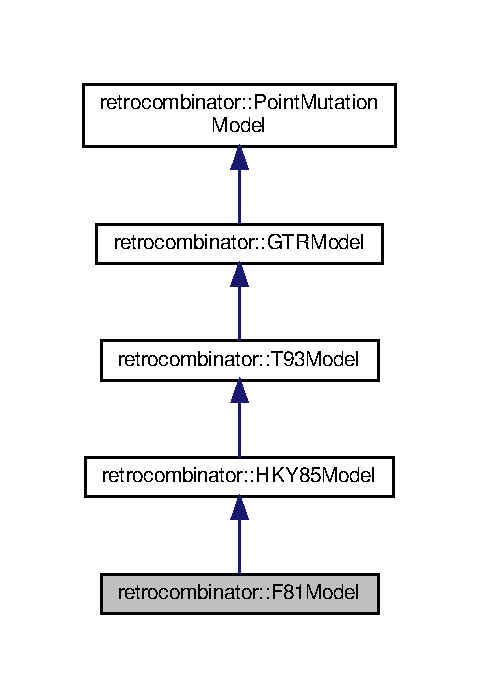
\includegraphics[width=230pt]{classretrocombinator_1_1F81Model__inherit__graph}
\end{center}
\end{figure}


Collaboration diagram for retrocombinator\+:\+:F81\+Model\+:
\nopagebreak
\begin{figure}[H]
\begin{center}
\leavevmode
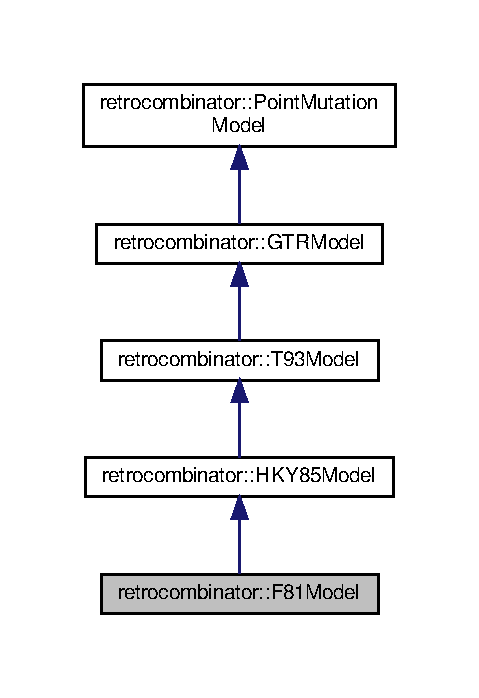
\includegraphics[width=230pt]{classretrocombinator_1_1F81Model__coll__graph}
\end{center}
\end{figure}
\subsection*{Public Member Functions}
\begin{DoxyCompactItemize}
\item 
\hyperlink{classretrocombinator_1_1F81Model_a80c3357497cdc6b91ff4c408750b47bb}{F81\+Model} (double \hyperlink{classretrocombinator_1_1GTRModel_ab002dbc62f8e8fbfc94558dd94166bd8}{pi\+\_\+T}=0.\+25, double pi\+\_\+C=0.\+25, double pi\+\_\+A=0.\+25, double pi\+\_\+G=0.\+25, double \hyperlink{classretrocombinator_1_1PointMutationModel_a3258dfbdae0f2614cdc66f13ae028b46}{scale}=1)
\begin{DoxyCompactList}\small\item\em 4 equilibrium base frequency parameters and 1 scale parameter. \end{DoxyCompactList}\end{DoxyCompactItemize}
\subsection*{Protected Member Functions}
\begin{DoxyCompactItemize}
\item 
\mbox{\Hypertarget{classretrocombinator_1_1F81Model_a5bb9c63e55c4f8f7b9573281ff6ee610}\label{classretrocombinator_1_1F81Model_a5bb9c63e55c4f8f7b9573281ff6ee610}} 
void \hyperlink{classretrocombinator_1_1F81Model_a5bb9c63e55c4f8f7b9573281ff6ee610}{compute\+\_\+transition\+\_\+matrix} () override
\begin{DoxyCompactList}\small\item\em Computed by exploiting symmetry. \end{DoxyCompactList}\end{DoxyCompactItemize}
\subsection*{Additional Inherited Members}


\subsection{Detailed Description}
Felsenstein 1981 Model. 

\subsection{Constructor \& Destructor Documentation}
\mbox{\Hypertarget{classretrocombinator_1_1F81Model_a80c3357497cdc6b91ff4c408750b47bb}\label{classretrocombinator_1_1F81Model_a80c3357497cdc6b91ff4c408750b47bb}} 
\index{retrocombinator\+::\+F81\+Model@{retrocombinator\+::\+F81\+Model}!F81\+Model@{F81\+Model}}
\index{F81\+Model@{F81\+Model}!retrocombinator\+::\+F81\+Model@{retrocombinator\+::\+F81\+Model}}
\subsubsection{\texorpdfstring{F81\+Model()}{F81Model()}}
{\footnotesize\ttfamily F81\+Model\+::\+F81\+Model (\begin{DoxyParamCaption}\item[{double}]{pi\+\_\+T = {\ttfamily 0.25},  }\item[{double}]{pi\+\_\+C = {\ttfamily 0.25},  }\item[{double}]{pi\+\_\+A = {\ttfamily 0.25},  }\item[{double}]{pi\+\_\+G = {\ttfamily 0.25},  }\item[{double}]{scale = {\ttfamily 1} }\end{DoxyParamCaption})}



4 equilibrium base frequency parameters and 1 scale parameter. 

pi\+\_\+X = same as for G\+TR scale = same as for G\+TR 

The documentation for this class was generated from the following files\+:\begin{DoxyCompactItemize}
\item 
src/\hyperlink{point__mutation__models_8h}{point\+\_\+mutation\+\_\+models.\+h}\item 
src/point\+\_\+mutation\+\_\+models.\+cpp\end{DoxyCompactItemize}

\hypertarget{classretrocombinator_1_1Family}{}\doxysection{retrocombinator\+::Family Class Reference}
\label{classretrocombinator_1_1Family}\index{retrocombinator::Family@{retrocombinator::Family}}


To store a set of sequences that can recombine with each other.  




{\ttfamily \#include $<$family.\+h$>$}

\doxysubsection*{Public Types}
\begin{DoxyCompactItemize}
\item 
typedef std\+::vector$<$ \mbox{\hyperlink{classretrocombinator_1_1Sequence}{Sequence}} $>$ \mbox{\hyperlink{classretrocombinator_1_1Family_a994b8646d1c0c4e19420d2e5c6c53c85}{seqs\+\_\+type}}
\begin{DoxyCompactList}\small\item\em The actual sequences in this family that can recombine with each other. \end{DoxyCompactList}\end{DoxyCompactItemize}
\doxysubsection*{Public Member Functions}
\begin{DoxyCompactItemize}
\item 
\mbox{\hyperlink{classretrocombinator_1_1Family_aefb8619ac695a3ad8e654ed8302668ee}{Family}} (\mbox{\hyperlink{namespaceretrocombinator_afd7c6eb4293e8c4d12827609a9a34b9b}{tag\+\_\+type}} \mbox{\hyperlink{classretrocombinator_1_1Family_aa5885cd6d63468db43859a860f7f16b4}{parent\+\_\+tag}})
\begin{DoxyCompactList}\small\item\em Constructor that takes the family that this was created from. \end{DoxyCompactList}\item 
\mbox{\Hypertarget{classretrocombinator_1_1Family_a0b767536f3a583fbeb77cadcdc1479b2}\label{classretrocombinator_1_1Family_a0b767536f3a583fbeb77cadcdc1479b2}} 
\mbox{\hyperlink{namespaceretrocombinator_a8e1541b50cee66a791df4c437ccbb385}{size\+\_\+type}} \mbox{\hyperlink{classretrocombinator_1_1Family_a0b767536f3a583fbeb77cadcdc1479b2}{size}} ()
\begin{DoxyCompactList}\small\item\em Gets the number of sequences in this family. \end{DoxyCompactList}\item 
\mbox{\Hypertarget{classretrocombinator_1_1Family_a11eab2ee12f8291620b230568ac3ab59}\label{classretrocombinator_1_1Family_a11eab2ee12f8291620b230568ac3ab59}} 
\mbox{\hyperlink{namespaceretrocombinator_afd7c6eb4293e8c4d12827609a9a34b9b}{tag\+\_\+type}} \mbox{\hyperlink{classretrocombinator_1_1Family_a11eab2ee12f8291620b230568ac3ab59}{get\+\_\+tag}} () const
\begin{DoxyCompactList}\small\item\em Gets the tag of this family. \end{DoxyCompactList}\item 
\mbox{\Hypertarget{classretrocombinator_1_1Family_a8f730b881fa67c9fc664ef293b46434b}\label{classretrocombinator_1_1Family_a8f730b881fa67c9fc664ef293b46434b}} 
\mbox{\hyperlink{namespaceretrocombinator_afd7c6eb4293e8c4d12827609a9a34b9b}{tag\+\_\+type}} \mbox{\hyperlink{classretrocombinator_1_1Family_a8f730b881fa67c9fc664ef293b46434b}{get\+\_\+parent\+\_\+tag}} () const
\begin{DoxyCompactList}\small\item\em Gets the tag of the parent family. \end{DoxyCompactList}\item 
void \mbox{\hyperlink{classretrocombinator_1_1Family_a721e453eb40fa49bd38ae24df001f9a3}{split}} ()
\begin{DoxyCompactList}\small\item\em When this family has split into subfamilies, update the tags. \end{DoxyCompactList}\end{DoxyCompactItemize}
\doxysubsection*{Static Public Member Functions}
\begin{DoxyCompactItemize}
\item 
static void \mbox{\hyperlink{classretrocombinator_1_1Family_a79b180c88225ee52d21da020375d2dfd}{renumber\+\_\+families}} (\mbox{\hyperlink{namespaceretrocombinator_afd7c6eb4293e8c4d12827609a9a34b9b}{tag\+\_\+type}} new\+\_\+start\+\_\+tag)
\begin{DoxyCompactList}\small\item\em Explicitly update the global family count to start from a particular number. \end{DoxyCompactList}\end{DoxyCompactItemize}
\doxysubsection*{Public Attributes}
\begin{DoxyCompactItemize}
\item 
\mbox{\Hypertarget{classretrocombinator_1_1Family_a61f3880b5481b4ace7f4b50f80df3738}\label{classretrocombinator_1_1Family_a61f3880b5481b4ace7f4b50f80df3738}} 
\mbox{\hyperlink{classretrocombinator_1_1Family_a994b8646d1c0c4e19420d2e5c6c53c85}{seqs\+\_\+type}} \mbox{\hyperlink{classretrocombinator_1_1Family_a61f3880b5481b4ace7f4b50f80df3738}{seqs}}
\begin{DoxyCompactList}\small\item\em The actual set of sequences. \end{DoxyCompactList}\end{DoxyCompactItemize}
\doxysubsection*{Private Attributes}
\begin{DoxyCompactItemize}
\item 
\mbox{\hyperlink{namespaceretrocombinator_afd7c6eb4293e8c4d12827609a9a34b9b}{tag\+\_\+type}} \mbox{\hyperlink{classretrocombinator_1_1Family_a50f0b448e39c126db2c12bdcac5a488d}{tag}}
\begin{DoxyCompactList}\small\item\em A tag that uniquely identifies this family. \end{DoxyCompactList}\item 
\mbox{\hyperlink{namespaceretrocombinator_afd7c6eb4293e8c4d12827609a9a34b9b}{tag\+\_\+type}} \mbox{\hyperlink{classretrocombinator_1_1Family_aa5885cd6d63468db43859a860f7f16b4}{parent\+\_\+tag}}
\begin{DoxyCompactList}\small\item\em The base family from which this family branched out from. \end{DoxyCompactList}\end{DoxyCompactItemize}
\doxysubsection*{Static Private Attributes}
\begin{DoxyCompactItemize}
\item 
static \mbox{\hyperlink{namespaceretrocombinator_afd7c6eb4293e8c4d12827609a9a34b9b}{tag\+\_\+type}} \mbox{\hyperlink{classretrocombinator_1_1Family_a957b56c44378b30bfeb0a8eebe9aa32d}{global\+\_\+family\+\_\+count}} = -\/1
\begin{DoxyCompactList}\small\item\em An internal counter that is incremented every time a family is created. \end{DoxyCompactList}\end{DoxyCompactItemize}


\doxysubsection{Detailed Description}
To store a set of sequences that can recombine with each other. 

\doxysubsection{Member Typedef Documentation}
\mbox{\Hypertarget{classretrocombinator_1_1Family_a994b8646d1c0c4e19420d2e5c6c53c85}\label{classretrocombinator_1_1Family_a994b8646d1c0c4e19420d2e5c6c53c85}} 
\index{retrocombinator::Family@{retrocombinator::Family}!seqs\_type@{seqs\_type}}
\index{seqs\_type@{seqs\_type}!retrocombinator::Family@{retrocombinator::Family}}
\doxysubsubsection{\texorpdfstring{seqs\_type}{seqs\_type}}
{\footnotesize\ttfamily typedef std\+::vector$<$\mbox{\hyperlink{classretrocombinator_1_1Sequence}{Sequence}}$>$ \mbox{\hyperlink{classretrocombinator_1_1Family_a994b8646d1c0c4e19420d2e5c6c53c85}{retrocombinator\+::\+Family\+::seqs\+\_\+type}}}



The actual sequences in this family that can recombine with each other. 

The container for a family of sequences 

\doxysubsection{Constructor \& Destructor Documentation}
\mbox{\Hypertarget{classretrocombinator_1_1Family_aefb8619ac695a3ad8e654ed8302668ee}\label{classretrocombinator_1_1Family_aefb8619ac695a3ad8e654ed8302668ee}} 
\index{retrocombinator::Family@{retrocombinator::Family}!Family@{Family}}
\index{Family@{Family}!retrocombinator::Family@{retrocombinator::Family}}
\doxysubsubsection{\texorpdfstring{Family()}{Family()}}
{\footnotesize\ttfamily Family\+::\+Family (\begin{DoxyParamCaption}\item[{\mbox{\hyperlink{namespaceretrocombinator_afd7c6eb4293e8c4d12827609a9a34b9b}{tag\+\_\+type}}}]{parent\+\_\+tag }\end{DoxyParamCaption})}



Constructor that takes the family that this was created from. 

If this was the initial family in a simulation, initialize with {\itshape \mbox{\hyperlink{namespaceretrocombinator_1_1Consts_af4adf5f1b75ede326285e110e2acf837}{Consts\+::\+I\+N\+I\+T\+\_\+\+F\+A\+M\+I\+L\+Y\+\_\+\+C\+O\+U\+NT}}}. 

\doxysubsection{Member Function Documentation}
\mbox{\Hypertarget{classretrocombinator_1_1Family_a79b180c88225ee52d21da020375d2dfd}\label{classretrocombinator_1_1Family_a79b180c88225ee52d21da020375d2dfd}} 
\index{retrocombinator::Family@{retrocombinator::Family}!renumber\_families@{renumber\_families}}
\index{renumber\_families@{renumber\_families}!retrocombinator::Family@{retrocombinator::Family}}
\doxysubsubsection{\texorpdfstring{renumber\_families()}{renumber\_families()}}
{\footnotesize\ttfamily void Family\+::renumber\+\_\+families (\begin{DoxyParamCaption}\item[{\mbox{\hyperlink{namespaceretrocombinator_afd7c6eb4293e8c4d12827609a9a34b9b}{tag\+\_\+type}}}]{new\+\_\+start\+\_\+tag }\end{DoxyParamCaption})\hspace{0.3cm}{\ttfamily [static]}}



Explicitly update the global family count to start from a particular number. 

new\+\_\+start\+\_\+tag will be given to the next family created. Used when running multiple simulations one after the other. Here is the caller graph for this function\+:
\nopagebreak
\begin{figure}[H]
\begin{center}
\leavevmode
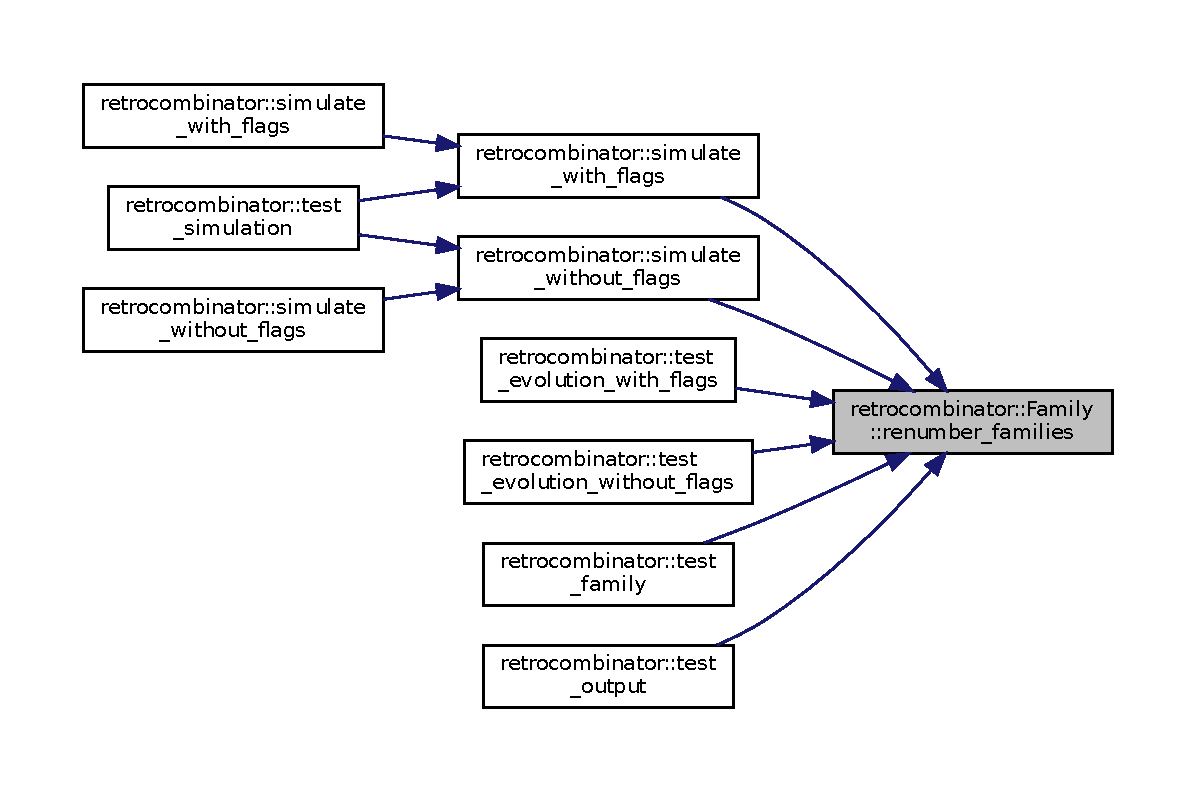
\includegraphics[width=350pt]{classretrocombinator_1_1Family_a79b180c88225ee52d21da020375d2dfd_icgraph}
\end{center}
\end{figure}
\mbox{\Hypertarget{classretrocombinator_1_1Family_a721e453eb40fa49bd38ae24df001f9a3}\label{classretrocombinator_1_1Family_a721e453eb40fa49bd38ae24df001f9a3}} 
\index{retrocombinator::Family@{retrocombinator::Family}!split@{split}}
\index{split@{split}!retrocombinator::Family@{retrocombinator::Family}}
\doxysubsubsection{\texorpdfstring{split()}{split()}}
{\footnotesize\ttfamily void Family\+::split (\begin{DoxyParamCaption}{ }\end{DoxyParamCaption})}



When this family has split into subfamilies, update the tags. 

Give it a new tag. Update its parent tag with the old tag. 

\doxysubsection{Member Data Documentation}
\mbox{\Hypertarget{classretrocombinator_1_1Family_a957b56c44378b30bfeb0a8eebe9aa32d}\label{classretrocombinator_1_1Family_a957b56c44378b30bfeb0a8eebe9aa32d}} 
\index{retrocombinator::Family@{retrocombinator::Family}!global\_family\_count@{global\_family\_count}}
\index{global\_family\_count@{global\_family\_count}!retrocombinator::Family@{retrocombinator::Family}}
\doxysubsubsection{\texorpdfstring{global\_family\_count}{global\_family\_count}}
{\footnotesize\ttfamily \mbox{\hyperlink{namespaceretrocombinator_afd7c6eb4293e8c4d12827609a9a34b9b}{tag\+\_\+type}} retrocombinator\+::\+Family\+::global\+\_\+family\+\_\+count = -\/1\hspace{0.3cm}{\ttfamily [static]}, {\ttfamily [private]}}



An internal counter that is incremented every time a family is created. 

Used to assign each family a unique tag. \mbox{\Hypertarget{classretrocombinator_1_1Family_aa5885cd6d63468db43859a860f7f16b4}\label{classretrocombinator_1_1Family_aa5885cd6d63468db43859a860f7f16b4}} 
\index{retrocombinator::Family@{retrocombinator::Family}!parent\_tag@{parent\_tag}}
\index{parent\_tag@{parent\_tag}!retrocombinator::Family@{retrocombinator::Family}}
\doxysubsubsection{\texorpdfstring{parent\_tag}{parent\_tag}}
{\footnotesize\ttfamily \mbox{\hyperlink{namespaceretrocombinator_afd7c6eb4293e8c4d12827609a9a34b9b}{tag\+\_\+type}} retrocombinator\+::\+Family\+::parent\+\_\+tag\hspace{0.3cm}{\ttfamily [private]}}



The base family from which this family branched out from. 

0 is considered to be the initial family for a simulation \mbox{\Hypertarget{classretrocombinator_1_1Family_a50f0b448e39c126db2c12bdcac5a488d}\label{classretrocombinator_1_1Family_a50f0b448e39c126db2c12bdcac5a488d}} 
\index{retrocombinator::Family@{retrocombinator::Family}!tag@{tag}}
\index{tag@{tag}!retrocombinator::Family@{retrocombinator::Family}}
\doxysubsubsection{\texorpdfstring{tag}{tag}}
{\footnotesize\ttfamily \mbox{\hyperlink{namespaceretrocombinator_afd7c6eb4293e8c4d12827609a9a34b9b}{tag\+\_\+type}} retrocombinator\+::\+Family\+::tag\hspace{0.3cm}{\ttfamily [private]}}



A tag that uniquely identifies this family. 

If families are deleted forever, this tag is never updated again in the same simulation. 

The documentation for this class was generated from the following files\+:\begin{DoxyCompactItemize}
\item 
src/\mbox{\hyperlink{family_8h}{family.\+h}}\item 
src/family.\+cpp\end{DoxyCompactItemize}

\hypertarget{classretrocombinator_1_1GTRModel}{}\section{retrocombinator\+:\+:G\+T\+R\+Model Class Reference}
\label{classretrocombinator_1_1GTRModel}\index{retrocombinator\+::\+G\+T\+R\+Model@{retrocombinator\+::\+G\+T\+R\+Model}}


General Time Reversible Model, Tavare 1986.  




{\ttfamily \#include $<$point\+\_\+mutation\+\_\+models.\+h$>$}



Inheritance diagram for retrocombinator\+:\+:G\+T\+R\+Model\+:\nopagebreak
\begin{figure}[H]
\begin{center}
\leavevmode
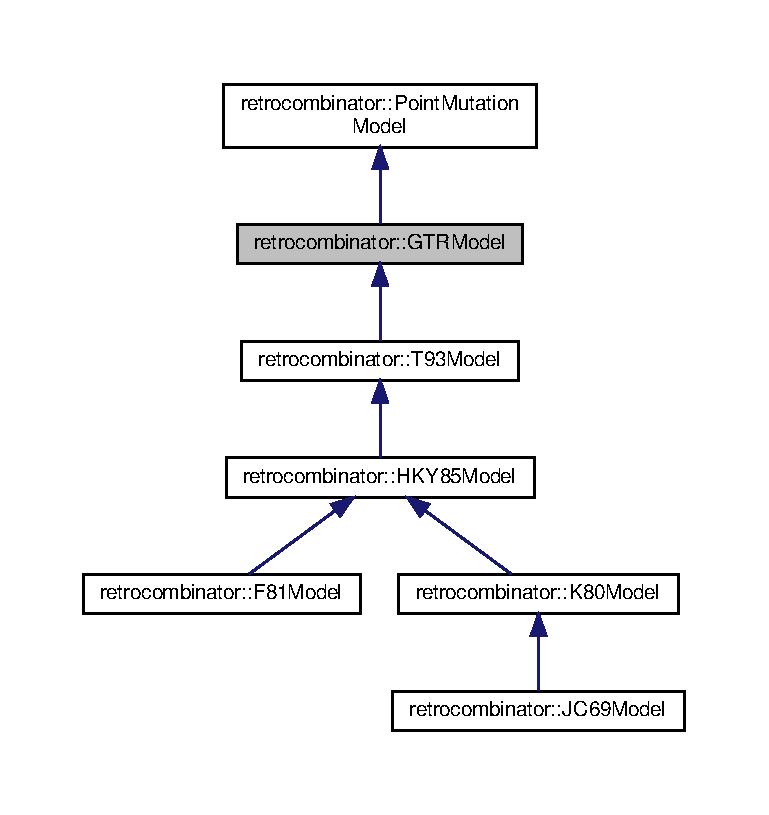
\includegraphics[width=350pt]{classretrocombinator_1_1GTRModel__inherit__graph}
\end{center}
\end{figure}


Collaboration diagram for retrocombinator\+:\+:G\+T\+R\+Model\+:\nopagebreak
\begin{figure}[H]
\begin{center}
\leavevmode
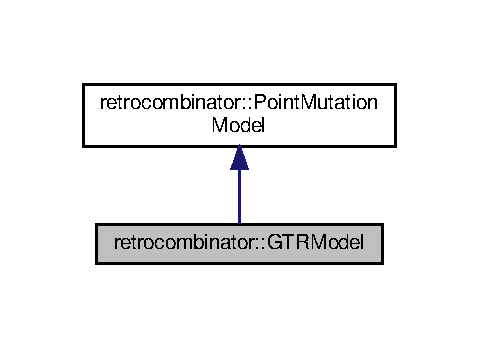
\includegraphics[width=230pt]{classretrocombinator_1_1GTRModel__coll__graph}
\end{center}
\end{figure}
\subsection*{Public Member Functions}
\begin{DoxyCompactItemize}
\item 
\hyperlink{classretrocombinator_1_1GTRModel_addd67a44caae9a477fc986d287dc2e8e}{G\+T\+R\+Model} (double \hyperlink{classretrocombinator_1_1GTRModel_ab002dbc62f8e8fbfc94558dd94166bd8}{pi\+\_\+T}=0.\+25, double pi\+\_\+C=0.\+25, double pi\+\_\+A=0.\+25, double pi\+\_\+G=0.\+25, double T2C=1, double T2A=1, double T2G=1, double C2A=1, double C2G=1, double A2G=1, double \hyperlink{classretrocombinator_1_1PointMutationModel_a3258dfbdae0f2614cdc66f13ae028b46}{scale}=1)
\begin{DoxyCompactList}\small\item\em 4 equilibrium base frequency parameters, 6 substitution rate parameters and 1 scale parameter. \end{DoxyCompactList}\end{DoxyCompactItemize}
\subsection*{Protected Member Functions}
\begin{DoxyCompactItemize}
\item 
\mbox{\Hypertarget{classretrocombinator_1_1GTRModel_a7d71f990fd33bcb7fc6a74accf03d7ae}\label{classretrocombinator_1_1GTRModel_a7d71f990fd33bcb7fc6a74accf03d7ae}} 
void \hyperlink{classretrocombinator_1_1GTRModel_a7d71f990fd33bcb7fc6a74accf03d7ae}{compute\+\_\+transition\+\_\+matrix} () override
\begin{DoxyCompactList}\small\item\em To be computed using exponentiation of Q. \end{DoxyCompactList}\end{DoxyCompactItemize}
\subsection*{Protected Attributes}
\textbf{ }\par
\begin{DoxyCompactItemize}
\item 
const double \hyperlink{classretrocombinator_1_1GTRModel_ab002dbc62f8e8fbfc94558dd94166bd8}{pi\+\_\+T}
\begin{DoxyCompactList}\small\item\em The base frequency parameters. \end{DoxyCompactList}\item 
\mbox{\Hypertarget{classretrocombinator_1_1GTRModel_a96e022540f373635aa6e381943a6c784}\label{classretrocombinator_1_1GTRModel_a96e022540f373635aa6e381943a6c784}} 
const double {\bfseries pi\+\_\+C}
\item 
\mbox{\Hypertarget{classretrocombinator_1_1GTRModel_a5d01f90292efd30b32d3196450fefd51}\label{classretrocombinator_1_1GTRModel_a5d01f90292efd30b32d3196450fefd51}} 
const double {\bfseries pi\+\_\+A}
\item 
\mbox{\Hypertarget{classretrocombinator_1_1GTRModel_a799b9eae55da958f079e0747f0a1602d}\label{classretrocombinator_1_1GTRModel_a799b9eae55da958f079e0747f0a1602d}} 
const double {\bfseries pi\+\_\+G}
\end{DoxyCompactItemize}

\subsection*{Additional Inherited Members}


\subsection{Detailed Description}
General Time Reversible Model, Tavare 1986. 

\subsection{Constructor \& Destructor Documentation}
\mbox{\Hypertarget{classretrocombinator_1_1GTRModel_addd67a44caae9a477fc986d287dc2e8e}\label{classretrocombinator_1_1GTRModel_addd67a44caae9a477fc986d287dc2e8e}} 
\index{retrocombinator\+::\+G\+T\+R\+Model@{retrocombinator\+::\+G\+T\+R\+Model}!G\+T\+R\+Model@{G\+T\+R\+Model}}
\index{G\+T\+R\+Model@{G\+T\+R\+Model}!retrocombinator\+::\+G\+T\+R\+Model@{retrocombinator\+::\+G\+T\+R\+Model}}
\subsubsection{\texorpdfstring{G\+T\+R\+Model()}{GTRModel()}}
{\footnotesize\ttfamily G\+T\+R\+Model\+::\+G\+T\+R\+Model (\begin{DoxyParamCaption}\item[{double}]{pi\+\_\+T = {\ttfamily 0.25},  }\item[{double}]{pi\+\_\+C = {\ttfamily 0.25},  }\item[{double}]{pi\+\_\+A = {\ttfamily 0.25},  }\item[{double}]{pi\+\_\+G = {\ttfamily 0.25},  }\item[{double}]{T2C = {\ttfamily 1},  }\item[{double}]{T2A = {\ttfamily 1},  }\item[{double}]{T2G = {\ttfamily 1},  }\item[{double}]{C2A = {\ttfamily 1},  }\item[{double}]{C2G = {\ttfamily 1},  }\item[{double}]{A2G = {\ttfamily 1},  }\item[{double}]{scale = {\ttfamily 1} }\end{DoxyParamCaption})}



4 equilibrium base frequency parameters, 6 substitution rate parameters and 1 scale parameter. 

pi\+\_\+X = equilibrium base frequencies X2Y = rate of X becoming Y scale = the scalar by which the matrix is to be scaled to get mutations/million years 

\subsection{Member Data Documentation}
\mbox{\Hypertarget{classretrocombinator_1_1GTRModel_ab002dbc62f8e8fbfc94558dd94166bd8}\label{classretrocombinator_1_1GTRModel_ab002dbc62f8e8fbfc94558dd94166bd8}} 
\index{retrocombinator\+::\+G\+T\+R\+Model@{retrocombinator\+::\+G\+T\+R\+Model}!pi\+\_\+T@{pi\+\_\+T}}
\index{pi\+\_\+T@{pi\+\_\+T}!retrocombinator\+::\+G\+T\+R\+Model@{retrocombinator\+::\+G\+T\+R\+Model}}
\subsubsection{\texorpdfstring{pi\+\_\+T}{pi\_T}}
{\footnotesize\ttfamily const double retrocombinator\+::\+G\+T\+R\+Model\+::pi\+\_\+T\hspace{0.3cm}{\ttfamily [protected]}}



The base frequency parameters. 

pi\+\_\+X is the proportion of the sequence that has nucleotide X after the system has reached equilibrium. 

The documentation for this class was generated from the following files\+:\begin{DoxyCompactItemize}
\item 
src/\hyperlink{point__mutation__models_8h}{point\+\_\+mutation\+\_\+models.\+h}\item 
src/point\+\_\+mutation\+\_\+models.\+cpp\end{DoxyCompactItemize}

\hypertarget{classretrocombinator_1_1HKY85Model}{}\doxysection{retrocombinator\+::H\+K\+Y85\+Model Class Reference}
\label{classretrocombinator_1_1HKY85Model}\index{retrocombinator::HKY85Model@{retrocombinator::HKY85Model}}


Hasegawa, Kishino and Yano 1985 Model.  




{\ttfamily \#include $<$point\+\_\+mutation\+\_\+models.\+h$>$}



Inheritance diagram for retrocombinator\+::H\+K\+Y85\+Model\+:
\nopagebreak
\begin{figure}[H]
\begin{center}
\leavevmode
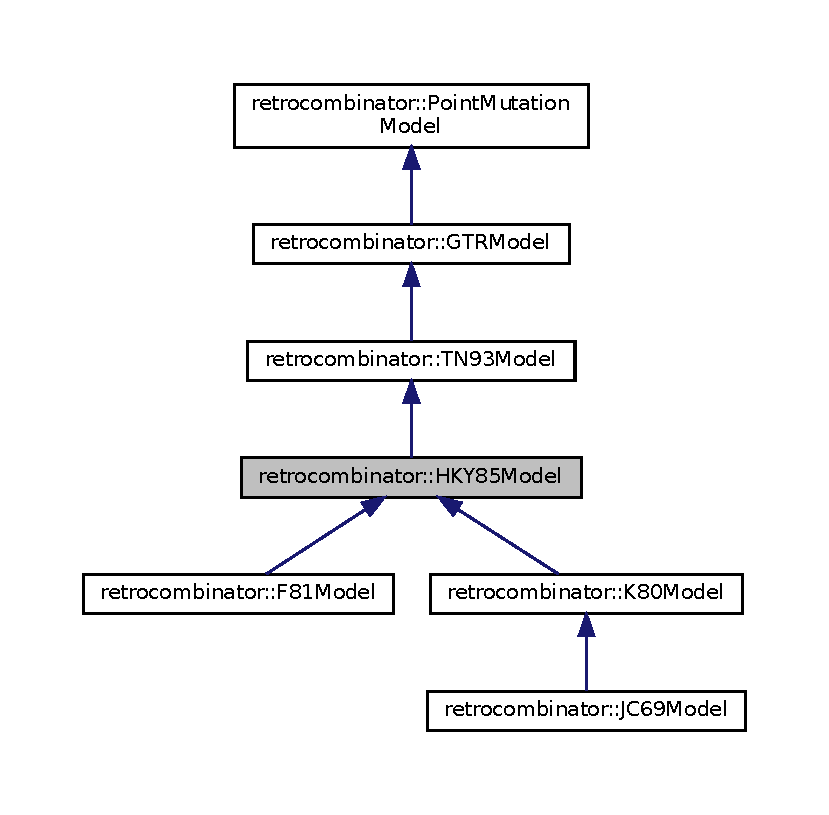
\includegraphics[width=350pt]{classretrocombinator_1_1HKY85Model__inherit__graph}
\end{center}
\end{figure}


Collaboration diagram for retrocombinator\+::H\+K\+Y85\+Model\+:
\nopagebreak
\begin{figure}[H]
\begin{center}
\leavevmode
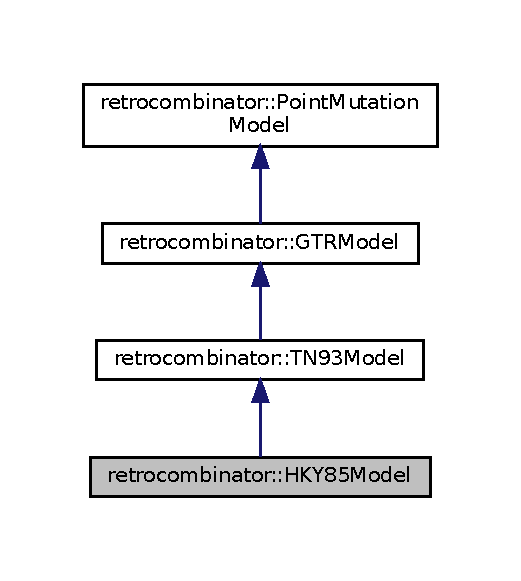
\includegraphics[width=250pt]{classretrocombinator_1_1HKY85Model__coll__graph}
\end{center}
\end{figure}
\doxysubsection*{Public Member Functions}
\begin{DoxyCompactItemize}
\item 
\mbox{\hyperlink{classretrocombinator_1_1HKY85Model_a2f4a296cdc444c92b54a4d972b044cdb}{H\+K\+Y85\+Model}} (double \mbox{\hyperlink{classretrocombinator_1_1GTRModel_ab002dbc62f8e8fbfc94558dd94166bd8}{pi\+\_\+T}}=0.\+25, double \mbox{\hyperlink{classretrocombinator_1_1GTRModel_a96e022540f373635aa6e381943a6c784}{pi\+\_\+C}}=0.\+25, double \mbox{\hyperlink{classretrocombinator_1_1GTRModel_a5d01f90292efd30b32d3196450fefd51}{pi\+\_\+A}}=0.\+25, double \mbox{\hyperlink{classretrocombinator_1_1GTRModel_a799b9eae55da958f079e0747f0a1602d}{pi\+\_\+G}}=0.\+25, double k=1, double \mbox{\hyperlink{classretrocombinator_1_1PointMutationModel_a3258dfbdae0f2614cdc66f13ae028b46}{scale}}=1)
\begin{DoxyCompactList}\small\item\em 4 equilibrium base frequency parameters, 1 substitution rate parameter and 1 scale parameter. \end{DoxyCompactList}\end{DoxyCompactItemize}
\doxysubsection*{Additional Inherited Members}


\doxysubsection{Detailed Description}
Hasegawa, Kishino and Yano 1985 Model. 

\doxysubsection{Constructor \& Destructor Documentation}
\mbox{\Hypertarget{classretrocombinator_1_1HKY85Model_a2f4a296cdc444c92b54a4d972b044cdb}\label{classretrocombinator_1_1HKY85Model_a2f4a296cdc444c92b54a4d972b044cdb}} 
\index{retrocombinator::HKY85Model@{retrocombinator::HKY85Model}!HKY85Model@{HKY85Model}}
\index{HKY85Model@{HKY85Model}!retrocombinator::HKY85Model@{retrocombinator::HKY85Model}}
\doxysubsubsection{\texorpdfstring{HKY85Model()}{HKY85Model()}}
{\footnotesize\ttfamily H\+K\+Y85\+Model\+::\+H\+K\+Y85\+Model (\begin{DoxyParamCaption}\item[{double}]{pi\+\_\+T = {\ttfamily 0.25},  }\item[{double}]{pi\+\_\+C = {\ttfamily 0.25},  }\item[{double}]{pi\+\_\+A = {\ttfamily 0.25},  }\item[{double}]{pi\+\_\+G = {\ttfamily 0.25},  }\item[{double}]{k = {\ttfamily 1},  }\item[{double}]{scale = {\ttfamily 1} }\end{DoxyParamCaption})}



4 equilibrium base frequency parameters, 1 substitution rate parameter and 1 scale parameter. 

pi\+\_\+X = same as for G\+TR k = rate of transitions(assuming rate of transversions is 1) scale = same as for G\+TR 

The documentation for this class was generated from the following files\+:\begin{DoxyCompactItemize}
\item 
src/\mbox{\hyperlink{point__mutation__models_8h}{point\+\_\+mutation\+\_\+models.\+h}}\item 
src/point\+\_\+mutation\+\_\+models.\+cpp\end{DoxyCompactItemize}

\hypertarget{classretrocombinator_1_1JC69Model}{}\doxysection{retrocombinator\+::J\+C69\+Model Class Reference}
\label{classretrocombinator_1_1JC69Model}\index{retrocombinator::JC69Model@{retrocombinator::JC69Model}}


Jules and Cantor, 1969.  




{\ttfamily \#include $<$point\+\_\+mutation\+\_\+models.\+h$>$}



Inheritance diagram for retrocombinator\+::J\+C69\+Model\+:\nopagebreak
\begin{figure}[H]
\begin{center}
\leavevmode
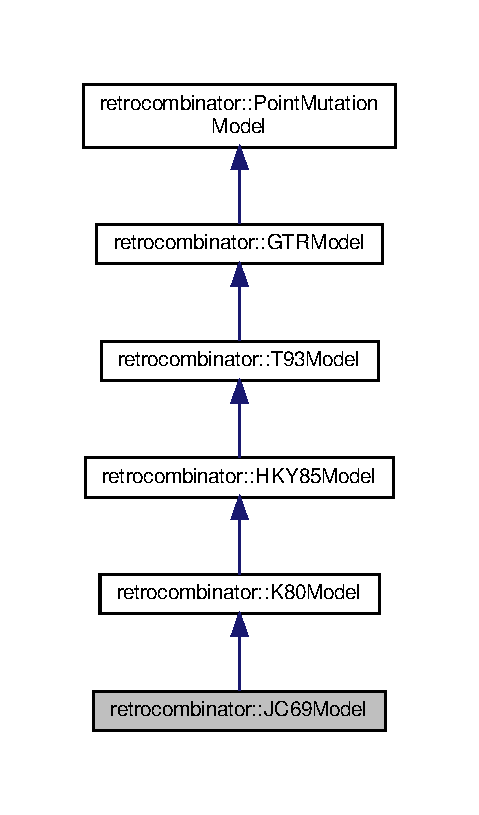
\includegraphics[width=250pt]{classretrocombinator_1_1JC69Model__inherit__graph}
\end{center}
\end{figure}


Collaboration diagram for retrocombinator\+::J\+C69\+Model\+:\nopagebreak
\begin{figure}[H]
\begin{center}
\leavevmode
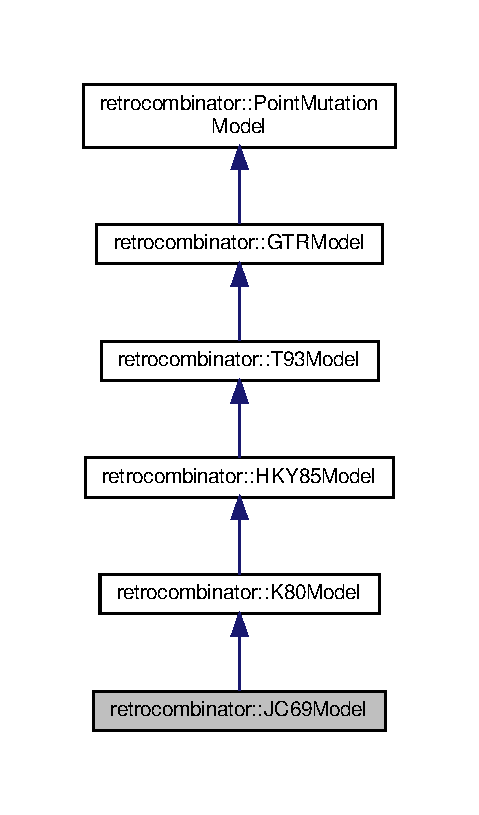
\includegraphics[width=250pt]{classretrocombinator_1_1JC69Model__coll__graph}
\end{center}
\end{figure}
\doxysubsection*{Public Member Functions}
\begin{DoxyCompactItemize}
\item 
\mbox{\hyperlink{classretrocombinator_1_1JC69Model_ab28021c22ed997738e2eac2f280930a5}{J\+C69\+Model}} (double \mbox{\hyperlink{classretrocombinator_1_1PointMutationModel_a3258dfbdae0f2614cdc66f13ae028b46}{scale}}=\mbox{\hyperlink{namespaceretrocombinator_1_1Consts_aeeeb7201b2611b428004059f329473ba}{Consts\+::\+J\+C69\+\_\+\+S\+C\+A\+LE}})
\begin{DoxyCompactList}\small\item\em 1 scale parameter. \end{DoxyCompactList}\end{DoxyCompactItemize}
\doxysubsection*{Additional Inherited Members}


\doxysubsection{Detailed Description}
Jules and Cantor, 1969. 

\doxysubsection{Constructor \& Destructor Documentation}
\mbox{\Hypertarget{classretrocombinator_1_1JC69Model_ab28021c22ed997738e2eac2f280930a5}\label{classretrocombinator_1_1JC69Model_ab28021c22ed997738e2eac2f280930a5}} 
\index{retrocombinator::JC69Model@{retrocombinator::JC69Model}!JC69Model@{JC69Model}}
\index{JC69Model@{JC69Model}!retrocombinator::JC69Model@{retrocombinator::JC69Model}}
\doxysubsubsection{\texorpdfstring{JC69Model()}{JC69Model()}}
{\footnotesize\ttfamily J\+C69\+Model\+::\+J\+C69\+Model (\begin{DoxyParamCaption}\item[{double}]{scale = {\ttfamily \mbox{\hyperlink{namespaceretrocombinator_1_1Consts_aeeeb7201b2611b428004059f329473ba}{Consts\+::\+J\+C69\+\_\+\+S\+C\+A\+LE}}} }\end{DoxyParamCaption})}



1 scale parameter. 

scale = same as for G\+TR 

The documentation for this class was generated from the following files\+:\begin{DoxyCompactItemize}
\item 
src/\mbox{\hyperlink{point__mutation__models_8h}{point\+\_\+mutation\+\_\+models.\+h}}\item 
src/point\+\_\+mutation\+\_\+models.\+cpp\end{DoxyCompactItemize}

\hypertarget{classretrocombinator_1_1K80Model}{}\doxysection{retrocombinator\+::K80\+Model Class Reference}
\label{classretrocombinator_1_1K80Model}\index{retrocombinator::K80Model@{retrocombinator::K80Model}}


Kimura 2 Parameter Model, 1980.  




{\ttfamily \#include $<$point\+\_\+mutation\+\_\+models.\+h$>$}



Inheritance diagram for retrocombinator\+::K80\+Model\+:\nopagebreak
\begin{figure}[H]
\begin{center}
\leavevmode
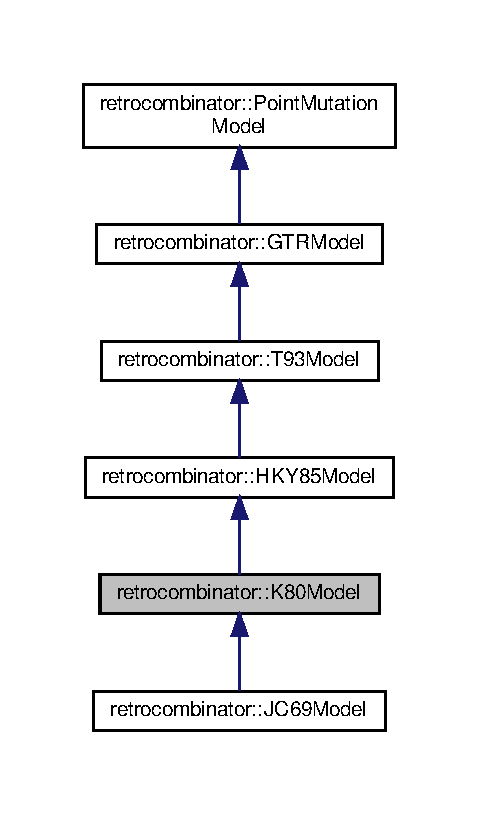
\includegraphics[width=250pt]{classretrocombinator_1_1K80Model__inherit__graph}
\end{center}
\end{figure}


Collaboration diagram for retrocombinator\+::K80\+Model\+:\nopagebreak
\begin{figure}[H]
\begin{center}
\leavevmode
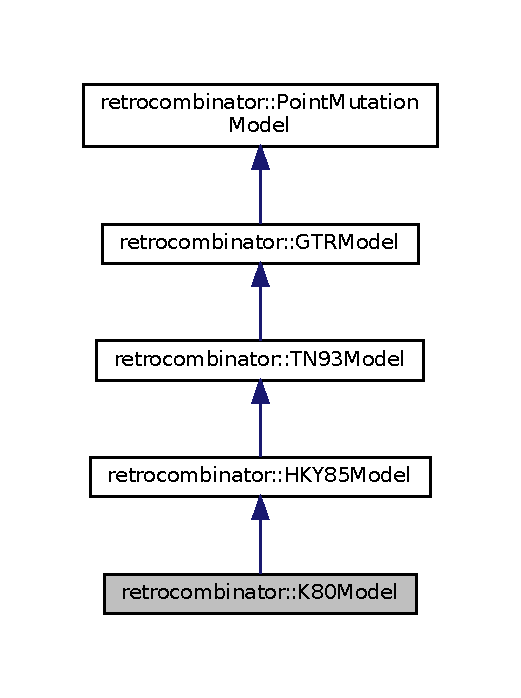
\includegraphics[width=250pt]{classretrocombinator_1_1K80Model__coll__graph}
\end{center}
\end{figure}
\doxysubsection*{Public Member Functions}
\begin{DoxyCompactItemize}
\item 
\mbox{\hyperlink{classretrocombinator_1_1K80Model_af199581e9a4d387f5e9e4f5bd048904b}{K80\+Model}} (double k=\mbox{\hyperlink{namespaceretrocombinator_1_1Consts_ac72fd4ec7b9dc3b42523a83cd69eaee2}{Consts\+::\+K80\+\_\+K}}, double \mbox{\hyperlink{classretrocombinator_1_1PointMutationModel_a3258dfbdae0f2614cdc66f13ae028b46}{scale}}=\mbox{\hyperlink{namespaceretrocombinator_1_1Consts_a49787213bbb5ff96754671440c758270}{Consts\+::\+K80\+\_\+\+S\+C\+A\+LE}})
\begin{DoxyCompactList}\small\item\em 1 substitution rate parameter and 1 scale parameter. \end{DoxyCompactList}\end{DoxyCompactItemize}
\doxysubsection*{Protected Member Functions}
\begin{DoxyCompactItemize}
\item 
\mbox{\Hypertarget{classretrocombinator_1_1K80Model_a70f669e2a31d34a37b19fd185219a9ce}\label{classretrocombinator_1_1K80Model_a70f669e2a31d34a37b19fd185219a9ce}} 
void \mbox{\hyperlink{classretrocombinator_1_1K80Model_a70f669e2a31d34a37b19fd185219a9ce}{compute\+\_\+transition\+\_\+matrix}} () override
\begin{DoxyCompactList}\small\item\em Computed by exploiting symmetry. \end{DoxyCompactList}\end{DoxyCompactItemize}
\doxysubsection*{Additional Inherited Members}


\doxysubsection{Detailed Description}
Kimura 2 Parameter Model, 1980. 

\doxysubsection{Constructor \& Destructor Documentation}
\mbox{\Hypertarget{classretrocombinator_1_1K80Model_af199581e9a4d387f5e9e4f5bd048904b}\label{classretrocombinator_1_1K80Model_af199581e9a4d387f5e9e4f5bd048904b}} 
\index{retrocombinator::K80Model@{retrocombinator::K80Model}!K80Model@{K80Model}}
\index{K80Model@{K80Model}!retrocombinator::K80Model@{retrocombinator::K80Model}}
\doxysubsubsection{\texorpdfstring{K80Model()}{K80Model()}}
{\footnotesize\ttfamily K80\+Model\+::\+K80\+Model (\begin{DoxyParamCaption}\item[{double}]{k = {\ttfamily \mbox{\hyperlink{namespaceretrocombinator_1_1Consts_ac72fd4ec7b9dc3b42523a83cd69eaee2}{Consts\+::\+K80\+\_\+K}}},  }\item[{double}]{scale = {\ttfamily \mbox{\hyperlink{namespaceretrocombinator_1_1Consts_a49787213bbb5ff96754671440c758270}{Consts\+::\+K80\+\_\+\+S\+C\+A\+LE}}} }\end{DoxyParamCaption})}



1 substitution rate parameter and 1 scale parameter. 

k = rate of transitions (assuming rate of transversions is 1) scale = same as for G\+TR 

The documentation for this class was generated from the following files\+:\begin{DoxyCompactItemize}
\item 
src/\mbox{\hyperlink{point__mutation__models_8h}{point\+\_\+mutation\+\_\+models.\+h}}\item 
src/point\+\_\+mutation\+\_\+models.\+cpp\end{DoxyCompactItemize}

\hypertarget{classretrocombinator_1_1Output}{}\section{retrocombinator\+:\+:Output Class Reference}
\label{classretrocombinator_1_1Output}\index{retrocombinator\+::\+Output@{retrocombinator\+::\+Output}}


Outputs the results of the simulation to a file.  




{\ttfamily \#include $<$output.\+h$>$}

\subsection*{Public Types}
\begin{DoxyCompactItemize}
\item 
\mbox{\Hypertarget{classretrocombinator_1_1Output_a2df584f5a2dbb2bf4a6789118902d83c}\label{classretrocombinator_1_1Output_a2df584f5a2dbb2bf4a6789118902d83c}} 
typedef \hyperlink{classretrocombinator_1_1Family_a994b8646d1c0c4e19420d2e5c6c53c85}{Family\+::seqs\+\_\+type} \hyperlink{classretrocombinator_1_1Output_a2df584f5a2dbb2bf4a6789118902d83c}{seqs\+\_\+type}
\begin{DoxyCompactList}\small\item\em Borrow typedef. \end{DoxyCompactList}\end{DoxyCompactItemize}
\subsection*{Public Member Functions}
\begin{DoxyCompactItemize}
\item 
\hyperlink{classretrocombinator_1_1Output_ac4dcc9e837413d0669f5b943f8d82dde}{Output} (const std\+::string \&filename\+\_\+out, \hyperlink{constants_8h_a8e1541b50cee66a791df4c437ccbb385}{size\+\_\+type} \hyperlink{classretrocombinator_1_1Output_a94f5e60b0aafcc409c78507c5e34ba7a}{final\+\_\+time}, \hyperlink{constants_8h_a8e1541b50cee66a791df4c437ccbb385}{size\+\_\+type} num\+\_\+out\+\_\+tags, \hyperlink{constants_8h_a8e1541b50cee66a791df4c437ccbb385}{size\+\_\+type} num\+\_\+out\+\_\+init, \hyperlink{constants_8h_a8e1541b50cee66a791df4c437ccbb385}{size\+\_\+type} num\+\_\+out\+\_\+seqs, \hyperlink{constants_8h_a8e1541b50cee66a791df4c437ccbb385}{size\+\_\+type} num\+\_\+out\+\_\+pair)
\begin{DoxyCompactList}\small\item\em Constructor, to specify how often we write to file. \end{DoxyCompactList}\item 
\mbox{\Hypertarget{classretrocombinator_1_1Output_a61d0840daf98bea49e4dc471f235eeab}\label{classretrocombinator_1_1Output_a61d0840daf98bea49e4dc471f235eeab}} 
\hyperlink{classretrocombinator_1_1Output_a61d0840daf98bea49e4dc471f235eeab}{$\sim$\+Output} ()
\begin{DoxyCompactList}\small\item\em Destructor to close the file and clean-\/up. \end{DoxyCompactList}\item 
\mbox{\Hypertarget{classretrocombinator_1_1Output_a5feb518230443e8259aeb3b12ecae437}\label{classretrocombinator_1_1Output_a5feb518230443e8259aeb3b12ecae437}} 
void \hyperlink{classretrocombinator_1_1Output_a5feb518230443e8259aeb3b12ecae437}{set\+\_\+init\+\_\+seq} (std\+::string \+\_\+init\+\_\+seq)
\begin{DoxyCompactList}\small\item\em This sets the sequence that we compare all sequences in our simulation against. \end{DoxyCompactList}\item 
\mbox{\Hypertarget{classretrocombinator_1_1Output_a210fa5a86077912c8cf95d15603c1ad2}\label{classretrocombinator_1_1Output_a210fa5a86077912c8cf95d15603c1ad2}} 
void \hyperlink{classretrocombinator_1_1Output_a210fa5a86077912c8cf95d15603c1ad2}{print\+\_\+header} ()
\begin{DoxyCompactList}\small\item\em Prints auxillary information regarding the simulation. \end{DoxyCompactList}\item 
\mbox{\Hypertarget{classretrocombinator_1_1Output_a9b28f297886b9e8f1e764b688c9a9da7}\label{classretrocombinator_1_1Output_a9b28f297886b9e8f1e764b688c9a9da7}} 
void \hyperlink{classretrocombinator_1_1Output_a9b28f297886b9e8f1e764b688c9a9da7}{print} (\hyperlink{constants_8h_a8e1541b50cee66a791df4c437ccbb385}{size\+\_\+type} timestep, double real\+\_\+time, const std\+::list$<$ \hyperlink{classretrocombinator_1_1Family}{Family} $>$ \&seqs)
\begin{DoxyCompactList}\small\item\em Prints the required information during the simulation. \end{DoxyCompactList}\end{DoxyCompactItemize}
\subsection*{Private Member Functions}
\textbf{ }\par
\begin{DoxyCompactItemize}
\item 
void \hyperlink{classretrocombinator_1_1Output_a365f66ac8299882ebfd6239d4c90b1bb}{print\+\_\+init} (const \hyperlink{classretrocombinator_1_1Output_a2df584f5a2dbb2bf4a6789118902d83c}{seqs\+\_\+type} \&seqs)
\begin{DoxyCompactList}\small\item\em Helper print functions. \end{DoxyCompactList}\item 
void \hyperlink{classretrocombinator_1_1Output_ac5632b57357788ba7d25769c412a2a11}{print\+\_\+pair} (const std\+::list$<$ \hyperlink{classretrocombinator_1_1Family}{Family} $>$ \&families)
\begin{DoxyCompactList}\small\item\em Prints pairwise distances across all families. \end{DoxyCompactList}\item 
\mbox{\Hypertarget{classretrocombinator_1_1Output_ac56d04591e50cbb8170da04a5ffa233a}\label{classretrocombinator_1_1Output_ac56d04591e50cbb8170da04a5ffa233a}} 
void \hyperlink{classretrocombinator_1_1Output_ac56d04591e50cbb8170da04a5ffa233a}{print\+\_\+seqs} (const \hyperlink{classretrocombinator_1_1Output_a2df584f5a2dbb2bf4a6789118902d83c}{seqs\+\_\+type} \&seqs)
\begin{DoxyCompactList}\small\item\em Prints raw sequences family-\/wise, in order. \end{DoxyCompactList}\item 
\mbox{\Hypertarget{classretrocombinator_1_1Output_a89392e3e01808946eaeb160955e87b21}\label{classretrocombinator_1_1Output_a89392e3e01808946eaeb160955e87b21}} 
void \hyperlink{classretrocombinator_1_1Output_a89392e3e01808946eaeb160955e87b21}{print\+\_\+seq\+\_\+tags} (const \hyperlink{classretrocombinator_1_1Output_a2df584f5a2dbb2bf4a6789118902d83c}{seqs\+\_\+type} \&seqs)
\begin{DoxyCompactList}\small\item\em Prints sequence tags family-\/wise, in order. \end{DoxyCompactList}\end{DoxyCompactItemize}

\subsection*{Private Attributes}
\begin{DoxyCompactItemize}
\item 
\mbox{\Hypertarget{classretrocombinator_1_1Output_a892712f42ff097ec7b3622fe88d7c441}\label{classretrocombinator_1_1Output_a892712f42ff097ec7b3622fe88d7c441}} 
std\+::fstream \hyperlink{classretrocombinator_1_1Output_a892712f42ff097ec7b3622fe88d7c441}{fout}
\begin{DoxyCompactList}\small\item\em A stream for the output. \end{DoxyCompactList}\item 
const \hyperlink{constants_8h_a8e1541b50cee66a791df4c437ccbb385}{size\+\_\+type} \hyperlink{classretrocombinator_1_1Output_a94f5e60b0aafcc409c78507c5e34ba7a}{final\+\_\+time}
\begin{DoxyCompactList}\small\item\em The final timestep in our simulation. \end{DoxyCompactList}\item 
\mbox{\Hypertarget{classretrocombinator_1_1Output_a338c2b8688791c8e1be4c5637e36f37f}\label{classretrocombinator_1_1Output_a338c2b8688791c8e1be4c5637e36f37f}} 
std\+::string \hyperlink{classretrocombinator_1_1Output_a338c2b8688791c8e1be4c5637e36f37f}{init\+\_\+seq}
\begin{DoxyCompactList}\small\item\em The initial sequence to compare to. \end{DoxyCompactList}\end{DoxyCompactItemize}
\textbf{ }\par
\begin{DoxyCompactItemize}
\item 
const \hyperlink{constants_8h_a8e1541b50cee66a791df4c437ccbb385}{size\+\_\+type} \hyperlink{classretrocombinator_1_1Output_a52a175aea7babe70c97021c0ccc47b4f}{to\+\_\+output\+\_\+tags}
\begin{DoxyCompactList}\small\item\em When to print out what data. \end{DoxyCompactList}\item 
\mbox{\Hypertarget{classretrocombinator_1_1Output_a63d41cf2393760562e67c8c20ea48120}\label{classretrocombinator_1_1Output_a63d41cf2393760562e67c8c20ea48120}} 
const \hyperlink{constants_8h_a8e1541b50cee66a791df4c437ccbb385}{size\+\_\+type} {\bfseries to\+\_\+output\+\_\+init}
\item 
\mbox{\Hypertarget{classretrocombinator_1_1Output_a9ac4938969e63a74c821463b4626eaa8}\label{classretrocombinator_1_1Output_a9ac4938969e63a74c821463b4626eaa8}} 
const \hyperlink{constants_8h_a8e1541b50cee66a791df4c437ccbb385}{size\+\_\+type} {\bfseries to\+\_\+output\+\_\+seqs}
\item 
\mbox{\Hypertarget{classretrocombinator_1_1Output_a54bab660e5cbe5c8f5dc60aa5df9c607}\label{classretrocombinator_1_1Output_a54bab660e5cbe5c8f5dc60aa5df9c607}} 
const \hyperlink{constants_8h_a8e1541b50cee66a791df4c437ccbb385}{size\+\_\+type} {\bfseries to\+\_\+output\+\_\+pair}
\end{DoxyCompactItemize}



\subsection{Detailed Description}
Outputs the results of the simulation to a file. 

Can output the following things at specified timesteps\+:
\begin{DoxyItemize}
\item The tags of the sequences and the families.
\item The raw sequences themselves.
\item The distance of each sequence to the inital sequence.
\item The pairwise distances between sequences. 
\end{DoxyItemize}

\subsection{Constructor \& Destructor Documentation}
\mbox{\Hypertarget{classretrocombinator_1_1Output_ac4dcc9e837413d0669f5b943f8d82dde}\label{classretrocombinator_1_1Output_ac4dcc9e837413d0669f5b943f8d82dde}} 
\index{retrocombinator\+::\+Output@{retrocombinator\+::\+Output}!Output@{Output}}
\index{Output@{Output}!retrocombinator\+::\+Output@{retrocombinator\+::\+Output}}
\subsubsection{\texorpdfstring{Output()}{Output()}}
{\footnotesize\ttfamily Output\+::\+Output (\begin{DoxyParamCaption}\item[{const std\+::string \&}]{filename\+\_\+out,  }\item[{\hyperlink{constants_8h_a8e1541b50cee66a791df4c437ccbb385}{size\+\_\+type}}]{final\+\_\+time,  }\item[{\hyperlink{constants_8h_a8e1541b50cee66a791df4c437ccbb385}{size\+\_\+type}}]{num\+\_\+out\+\_\+tags,  }\item[{\hyperlink{constants_8h_a8e1541b50cee66a791df4c437ccbb385}{size\+\_\+type}}]{num\+\_\+out\+\_\+init,  }\item[{\hyperlink{constants_8h_a8e1541b50cee66a791df4c437ccbb385}{size\+\_\+type}}]{num\+\_\+out\+\_\+seqs,  }\item[{\hyperlink{constants_8h_a8e1541b50cee66a791df4c437ccbb385}{size\+\_\+type}}]{num\+\_\+out\+\_\+pair }\end{DoxyParamCaption})}



Constructor, to specify how often we write to file. 

{\ttfamily num\+\_\+out\+\_\+X} = {\itshape n} means that the \textquotesingle{}X\textquotesingle{} output will occur {\itshape n} times. Look at the definitions of print\+\_\+\textquotesingle{}X\textquotesingle{} to learn what \textquotesingle{}X\textquotesingle{} is. 

\subsection{Member Function Documentation}
\mbox{\Hypertarget{classretrocombinator_1_1Output_a365f66ac8299882ebfd6239d4c90b1bb}\label{classretrocombinator_1_1Output_a365f66ac8299882ebfd6239d4c90b1bb}} 
\index{retrocombinator\+::\+Output@{retrocombinator\+::\+Output}!print\+\_\+init@{print\+\_\+init}}
\index{print\+\_\+init@{print\+\_\+init}!retrocombinator\+::\+Output@{retrocombinator\+::\+Output}}
\subsubsection{\texorpdfstring{print\+\_\+init()}{print\_init()}}
{\footnotesize\ttfamily void Output\+::print\+\_\+init (\begin{DoxyParamCaption}\item[{const \hyperlink{classretrocombinator_1_1Output_a2df584f5a2dbb2bf4a6789118902d83c}{seqs\+\_\+type} \&}]{seqs }\end{DoxyParamCaption})\hspace{0.3cm}{\ttfamily [private]}}



Helper print functions. 

tags\+: the tags of all sequences$\ast$ init\+: display distance to inital sequence$\ast$$\ast$ seqs\+: display raw sequences pair\+: display pairwise distances between the sequences

N\+O\+T\+ES\+:
\begin{DoxyItemize}
\item tags is always printed if something else is to be printed $\ast$$\ast$ init is always printed if seqs is to be printed\+Prints distance to initial sequence family-\/wise, in order 
\end{DoxyItemize}Here is the caller graph for this function\+:
\nopagebreak
\begin{figure}[H]
\begin{center}
\leavevmode
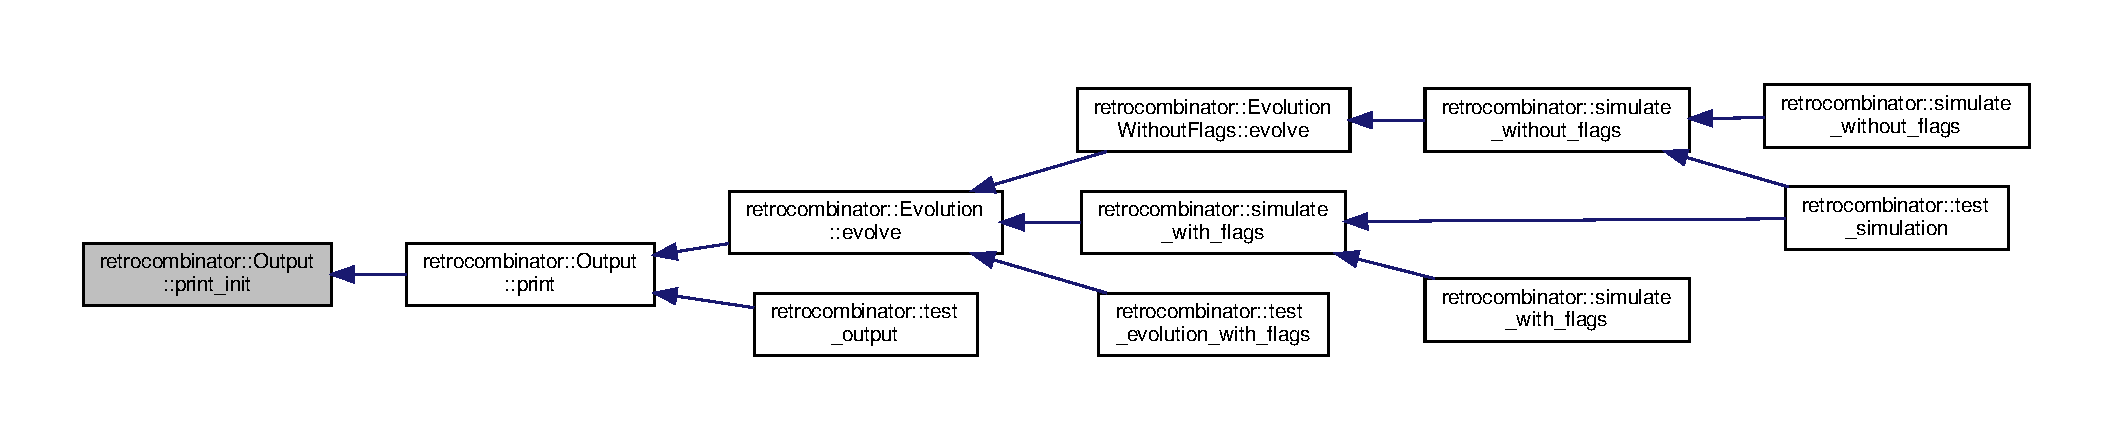
\includegraphics[width=350pt]{classretrocombinator_1_1Output_a365f66ac8299882ebfd6239d4c90b1bb_icgraph}
\end{center}
\end{figure}
\mbox{\Hypertarget{classretrocombinator_1_1Output_ac5632b57357788ba7d25769c412a2a11}\label{classretrocombinator_1_1Output_ac5632b57357788ba7d25769c412a2a11}} 
\index{retrocombinator\+::\+Output@{retrocombinator\+::\+Output}!print\+\_\+pair@{print\+\_\+pair}}
\index{print\+\_\+pair@{print\+\_\+pair}!retrocombinator\+::\+Output@{retrocombinator\+::\+Output}}
\subsubsection{\texorpdfstring{print\+\_\+pair()}{print\_pair()}}
{\footnotesize\ttfamily void Output\+::print\+\_\+pair (\begin{DoxyParamCaption}\item[{const std\+::list$<$ \hyperlink{classretrocombinator_1_1Family}{Family} $>$ \&}]{families }\end{DoxyParamCaption})\hspace{0.3cm}{\ttfamily [private]}}



Prints pairwise distances across all families. 

The order is as follows\+: for each family F1\+: for each seq S1 in F1\+: for each other seq S2 in F1\+: print S1$\ast$\+S2 for each other family F2\+: for each seq S2 in F2\+: print S1$\ast$\+S2 Here is the caller graph for this function\+:
\nopagebreak
\begin{figure}[H]
\begin{center}
\leavevmode
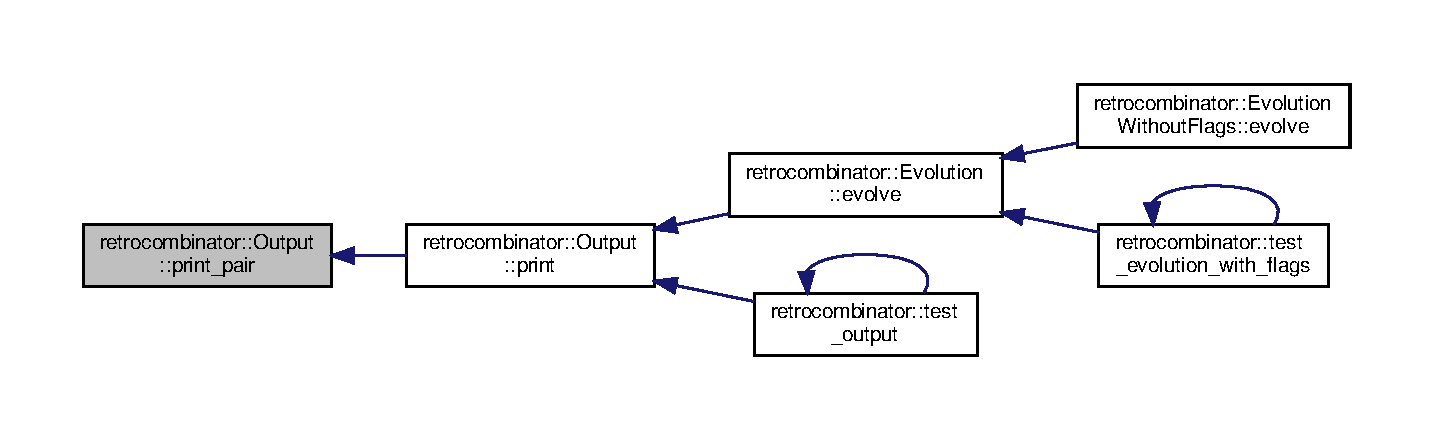
\includegraphics[width=350pt]{classretrocombinator_1_1Output_ac5632b57357788ba7d25769c412a2a11_icgraph}
\end{center}
\end{figure}


\subsection{Member Data Documentation}
\mbox{\Hypertarget{classretrocombinator_1_1Output_a94f5e60b0aafcc409c78507c5e34ba7a}\label{classretrocombinator_1_1Output_a94f5e60b0aafcc409c78507c5e34ba7a}} 
\index{retrocombinator\+::\+Output@{retrocombinator\+::\+Output}!final\+\_\+time@{final\+\_\+time}}
\index{final\+\_\+time@{final\+\_\+time}!retrocombinator\+::\+Output@{retrocombinator\+::\+Output}}
\subsubsection{\texorpdfstring{final\+\_\+time}{final\_time}}
{\footnotesize\ttfamily const \hyperlink{constants_8h_a8e1541b50cee66a791df4c437ccbb385}{size\+\_\+type} retrocombinator\+::\+Output\+::final\+\_\+time\hspace{0.3cm}{\ttfamily [private]}}



The final timestep in our simulation. 

Make sure we output everything we can at this timestep, regardless of what we explicity said should be output. \mbox{\Hypertarget{classretrocombinator_1_1Output_a52a175aea7babe70c97021c0ccc47b4f}\label{classretrocombinator_1_1Output_a52a175aea7babe70c97021c0ccc47b4f}} 
\index{retrocombinator\+::\+Output@{retrocombinator\+::\+Output}!to\+\_\+output\+\_\+tags@{to\+\_\+output\+\_\+tags}}
\index{to\+\_\+output\+\_\+tags@{to\+\_\+output\+\_\+tags}!retrocombinator\+::\+Output@{retrocombinator\+::\+Output}}
\subsubsection{\texorpdfstring{to\+\_\+output\+\_\+tags}{to\_output\_tags}}
{\footnotesize\ttfamily const \hyperlink{constants_8h_a8e1541b50cee66a791df4c437ccbb385}{size\+\_\+type} retrocombinator\+::\+Output\+::to\+\_\+output\+\_\+tags\hspace{0.3cm}{\ttfamily [private]}}



When to print out what data. 


\begin{DoxyItemize}
\item Only output X if {\ttfamily to\+\_\+output\+\_\+X} is a multiple of the current timestep in the simulation
\item Look at the definition of print\+\_\+\textquotesingle{}X\textquotesingle{} to learn what \textquotesingle{}X\textquotesingle{} is. 
\end{DoxyItemize}

The documentation for this class was generated from the following files\+:\begin{DoxyCompactItemize}
\item 
src/\hyperlink{output_8h}{output.\+h}\item 
src/output.\+cpp\end{DoxyCompactItemize}

\hypertarget{classretrocombinator_1_1PointMutationModel}{}\doxysection{retrocombinator\+::Point\+Mutation\+Model Class Reference}
\label{classretrocombinator_1_1PointMutationModel}\index{retrocombinator::PointMutationModel@{retrocombinator::PointMutationModel}}


To represent a model of D\+NA evolution through point mutations.  




{\ttfamily \#include $<$point\+\_\+mutation\+\_\+models.\+h$>$}



Inheritance diagram for retrocombinator\+::Point\+Mutation\+Model\+:\nopagebreak
\begin{figure}[H]
\begin{center}
\leavevmode
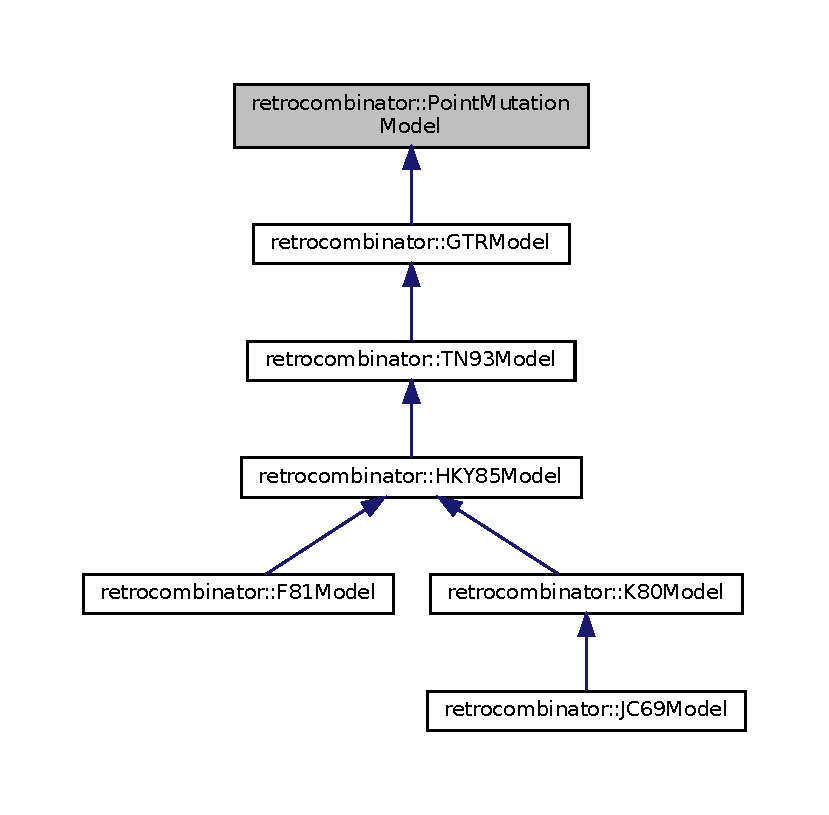
\includegraphics[width=350pt]{classretrocombinator_1_1PointMutationModel__inherit__graph}
\end{center}
\end{figure}
\doxysubsection*{Public Member Functions}
\begin{DoxyCompactItemize}
\item 
\mbox{\Hypertarget{classretrocombinator_1_1PointMutationModel_a4c83f671b3d76f8cf39ae5b5a1be658e}\label{classretrocombinator_1_1PointMutationModel_a4c83f671b3d76f8cf39ae5b5a1be658e}} 
\mbox{\hyperlink{classretrocombinator_1_1PointMutationModel_a4c83f671b3d76f8cf39ae5b5a1be658e}{Point\+Mutation\+Model}} (double \mbox{\hyperlink{classretrocombinator_1_1PointMutationModel_a3258dfbdae0f2614cdc66f13ae028b46}{scale}}=1)
\begin{DoxyCompactList}\small\item\em Constructor that allocates memory for transition matrix. \end{DoxyCompactList}\item 
virtual \mbox{\hyperlink{classretrocombinator_1_1PointMutationModel_a86a21482afab3faa92b5b05153c92915}{$\sim$\+Point\+Mutation\+Model}} ()=default
\begin{DoxyCompactList}\small\item\em Use the default destructor. \end{DoxyCompactList}\end{DoxyCompactItemize}
\doxysubsection*{Public Attributes}
\begin{DoxyCompactItemize}
\item 
\mbox{\hyperlink{namespaceretrocombinator_a04664f475f33337cf2a7a4a0b0e3125c}{Returns\+Nuc\+Matrix}} \mbox{\hyperlink{classretrocombinator_1_1PointMutationModel_a6c6e94bfbf16c3893068e3db1597e941}{get\+\_\+Q}}
\begin{DoxyCompactList}\small\item\em Returns a rate matrix for the mutations. \end{DoxyCompactList}\item 
\mbox{\hyperlink{namespaceretrocombinator_a4cbfa6c71aed12291a2875e9f4ce1438}{Returns\+Nuc\+Matrix\+From\+Double}} \mbox{\hyperlink{classretrocombinator_1_1PointMutationModel_a5f17e2f93b22723721a4d04ac2c77aaa}{get\+\_\+transition\+\_\+matrix}}
\begin{DoxyCompactList}\small\item\em Returns a transition matrix to represent the probabilities of mutations from each nucleotide to the other. \end{DoxyCompactList}\end{DoxyCompactItemize}
\doxysubsection*{Protected Member Functions}
\begin{DoxyCompactItemize}
\item 
virtual void \mbox{\hyperlink{classretrocombinator_1_1PointMutationModel_a29357db0a7cfb35ab1540840aa4cfda1}{compute\+\_\+transition\+\_\+matrix}} ()=0
\begin{DoxyCompactList}\small\item\em Computes Q from P using t\+\_\+stored. \end{DoxyCompactList}\end{DoxyCompactItemize}
\doxysubsection*{Protected Attributes}
\begin{DoxyCompactItemize}
\item 
\mbox{\Hypertarget{classretrocombinator_1_1PointMutationModel_a3f52ae4a94cb8a8cf75113f8b4a7a570}\label{classretrocombinator_1_1PointMutationModel_a3f52ae4a94cb8a8cf75113f8b4a7a570}} 
\mbox{\hyperlink{namespaceretrocombinator_a47bcd6dd938a6f8e34b0996d940f81ef}{Nuc\+Matrix}} \mbox{\hyperlink{classretrocombinator_1_1PointMutationModel_a3f52ae4a94cb8a8cf75113f8b4a7a570}{Q}}
\begin{DoxyCompactList}\small\item\em The transition rate matrix (unscaled) \end{DoxyCompactList}\item 
\mbox{\Hypertarget{classretrocombinator_1_1PointMutationModel_a3717e58e2be7cbfebffea2081dcf9663}\label{classretrocombinator_1_1PointMutationModel_a3717e58e2be7cbfebffea2081dcf9663}} 
\mbox{\hyperlink{namespaceretrocombinator_a47bcd6dd938a6f8e34b0996d940f81ef}{Nuc\+Matrix}} \mbox{\hyperlink{classretrocombinator_1_1PointMutationModel_a3717e58e2be7cbfebffea2081dcf9663}{P}}
\begin{DoxyCompactList}\small\item\em The transition matrix for times\+\_\+per\+\_\+step {\itshape t\+\_\+stored}. \end{DoxyCompactList}\item 
\mbox{\Hypertarget{classretrocombinator_1_1PointMutationModel_a3258dfbdae0f2614cdc66f13ae028b46}\label{classretrocombinator_1_1PointMutationModel_a3258dfbdae0f2614cdc66f13ae028b46}} 
double \mbox{\hyperlink{classretrocombinator_1_1PointMutationModel_a3258dfbdae0f2614cdc66f13ae028b46}{scale}}
\begin{DoxyCompactList}\small\item\em P = exp(scale $\ast$ Q $\ast$ time) \end{DoxyCompactList}\item 
\mbox{\Hypertarget{classretrocombinator_1_1PointMutationModel_a677f67cf3336af8aa105e60ee991bd13}\label{classretrocombinator_1_1PointMutationModel_a677f67cf3336af8aa105e60ee991bd13}} 
double \mbox{\hyperlink{classretrocombinator_1_1PointMutationModel_a677f67cf3336af8aa105e60ee991bd13}{t\+\_\+stored}}
\begin{DoxyCompactList}\small\item\em The time\+\_\+per\+\_\+step jump for which our transition matrix is valid. \end{DoxyCompactList}\end{DoxyCompactItemize}


\doxysubsection{Detailed Description}
To represent a model of D\+NA evolution through point mutations. 

\doxysubsection{Constructor \& Destructor Documentation}
\mbox{\Hypertarget{classretrocombinator_1_1PointMutationModel_a86a21482afab3faa92b5b05153c92915}\label{classretrocombinator_1_1PointMutationModel_a86a21482afab3faa92b5b05153c92915}} 
\index{retrocombinator::PointMutationModel@{retrocombinator::PointMutationModel}!````~PointMutationModel@{$\sim$PointMutationModel}}
\index{````~PointMutationModel@{$\sim$PointMutationModel}!retrocombinator::PointMutationModel@{retrocombinator::PointMutationModel}}
\doxysubsubsection{\texorpdfstring{$\sim$PointMutationModel()}{~PointMutationModel()}}
{\footnotesize\ttfamily virtual retrocombinator\+::\+Point\+Mutation\+Model\+::$\sim$\+Point\+Mutation\+Model (\begin{DoxyParamCaption}{ }\end{DoxyParamCaption})\hspace{0.3cm}{\ttfamily [virtual]}, {\ttfamily [default]}}



Use the default destructor. 

Is virtual because we want all specific point mutation models to derive from this class. 

\doxysubsection{Member Function Documentation}
\mbox{\Hypertarget{classretrocombinator_1_1PointMutationModel_a29357db0a7cfb35ab1540840aa4cfda1}\label{classretrocombinator_1_1PointMutationModel_a29357db0a7cfb35ab1540840aa4cfda1}} 
\index{retrocombinator::PointMutationModel@{retrocombinator::PointMutationModel}!compute\_transition\_matrix@{compute\_transition\_matrix}}
\index{compute\_transition\_matrix@{compute\_transition\_matrix}!retrocombinator::PointMutationModel@{retrocombinator::PointMutationModel}}
\doxysubsubsection{\texorpdfstring{compute\_transition\_matrix()}{compute\_transition\_matrix()}}
{\footnotesize\ttfamily virtual void retrocombinator\+::\+Point\+Mutation\+Model\+::compute\+\_\+transition\+\_\+matrix (\begin{DoxyParamCaption}{ }\end{DoxyParamCaption})\hspace{0.3cm}{\ttfamily [protected]}, {\ttfamily [pure virtual]}}



Computes Q from P using t\+\_\+stored. 

P(t) = exp(scale$\ast$\+Qt) 

Implemented in \mbox{\hyperlink{classretrocombinator_1_1K80Model_a70f669e2a31d34a37b19fd185219a9ce}{retrocombinator\+::\+K80\+Model}}, \mbox{\hyperlink{classretrocombinator_1_1F81Model_a5bb9c63e55c4f8f7b9573281ff6ee610}{retrocombinator\+::\+F81\+Model}}, \mbox{\hyperlink{classretrocombinator_1_1TN93Model_a169984ef7a2115229836b4988b83969e}{retrocombinator\+::\+T\+N93\+Model}}, and \mbox{\hyperlink{classretrocombinator_1_1GTRModel_a7d71f990fd33bcb7fc6a74accf03d7ae}{retrocombinator\+::\+G\+T\+R\+Model}}.



\doxysubsection{Member Data Documentation}
\mbox{\Hypertarget{classretrocombinator_1_1PointMutationModel_a6c6e94bfbf16c3893068e3db1597e941}\label{classretrocombinator_1_1PointMutationModel_a6c6e94bfbf16c3893068e3db1597e941}} 
\index{retrocombinator::PointMutationModel@{retrocombinator::PointMutationModel}!get\_Q@{get\_Q}}
\index{get\_Q@{get\_Q}!retrocombinator::PointMutationModel@{retrocombinator::PointMutationModel}}
\doxysubsubsection{\texorpdfstring{get\_Q}{get\_Q}}
{\footnotesize\ttfamily const double($\ast$ Point\+Mutation\+Model\+::get\+\_\+Q}



Returns a rate matrix for the mutations. 

After {\itshape t} years have passed, the probability is exp(rate$\ast$t). \mbox{\Hypertarget{classretrocombinator_1_1PointMutationModel_a5f17e2f93b22723721a4d04ac2c77aaa}\label{classretrocombinator_1_1PointMutationModel_a5f17e2f93b22723721a4d04ac2c77aaa}} 
\index{retrocombinator::PointMutationModel@{retrocombinator::PointMutationModel}!get\_transition\_matrix@{get\_transition\_matrix}}
\index{get\_transition\_matrix@{get\_transition\_matrix}!retrocombinator::PointMutationModel@{retrocombinator::PointMutationModel}}
\doxysubsubsection{\texorpdfstring{get\_transition\_matrix}{get\_transition\_matrix}}
{\footnotesize\ttfamily const double($\ast$ Point\+Mutation\+Model\+::get\+\_\+transition\+\_\+matrix}



Returns a transition matrix to represent the probabilities of mutations from each nucleotide to the other. 

{\itshape t} is the time that has passed in millions of years. P(\+A to B) is matrix(\+A, B). 

The documentation for this class was generated from the following files\+:\begin{DoxyCompactItemize}
\item 
src/\mbox{\hyperlink{point__mutation__models_8h}{point\+\_\+mutation\+\_\+models.\+h}}\item 
src/point\+\_\+mutation\+\_\+models.\+cpp\end{DoxyCompactItemize}

\hypertarget{classretrocombinator_1_1PointMutator}{}\doxysection{retrocombinator\+::Point\+Mutator Class Reference}
\label{classretrocombinator_1_1PointMutator}\index{retrocombinator::PointMutator@{retrocombinator::PointMutator}}


A class that can mutate a given sequence according to a specified point mutation model.  




{\ttfamily \#include $<$point\+\_\+mutator.\+h$>$}



Collaboration diagram for retrocombinator\+::Point\+Mutator\+:
\nopagebreak
\begin{figure}[H]
\begin{center}
\leavevmode
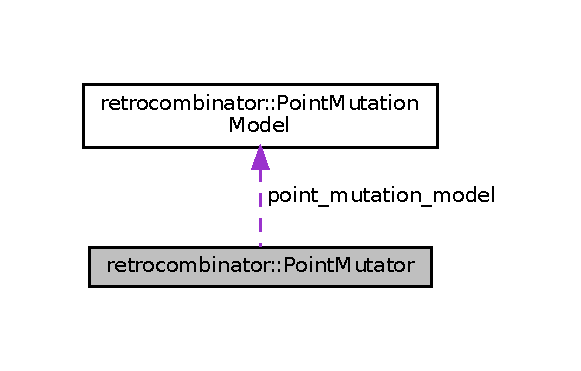
\includegraphics[width=279pt]{classretrocombinator_1_1PointMutator__coll__graph}
\end{center}
\end{figure}
\doxysubsection*{Public Member Functions}
\begin{DoxyCompactItemize}
\item 
\mbox{\Hypertarget{classretrocombinator_1_1PointMutator_a084f37ad47f0a820028a87695bd2c88e}\label{classretrocombinator_1_1PointMutator_a084f37ad47f0a820028a87695bd2c88e}} 
\mbox{\hyperlink{classretrocombinator_1_1PointMutator_a084f37ad47f0a820028a87695bd2c88e}{Point\+Mutator}} (std\+::string model, \mbox{\hyperlink{namespaceretrocombinator_a8e1541b50cee66a791df4c437ccbb385}{size\+\_\+type}} n, \mbox{\hyperlink{namespaceretrocombinator_a8e1541b50cee66a791df4c437ccbb385}{size\+\_\+type}} num\+\_\+sensitive\+\_\+posns=0, double inactive\+\_\+probability=0.\+0)
\begin{DoxyCompactList}\small\item\em Constructor that chooses a point mutation model and the probabilities for lethal mutations at each position in the sequence. \end{DoxyCompactList}\item 
\mbox{\Hypertarget{classretrocombinator_1_1PointMutator_ab4bb79937f1824e7fba92fb824f27c56}\label{classretrocombinator_1_1PointMutator_ab4bb79937f1824e7fba92fb824f27c56}} 
\mbox{\hyperlink{classretrocombinator_1_1PointMutator_ab4bb79937f1824e7fba92fb824f27c56}{$\sim$\+Point\+Mutator}} ()
\begin{DoxyCompactList}\small\item\em Destructor that frees up memory. \end{DoxyCompactList}\item 
\mbox{\Hypertarget{classretrocombinator_1_1PointMutator_aba3c2b8641affe8a06d815c33cafdc1b}\label{classretrocombinator_1_1PointMutator_aba3c2b8641affe8a06d815c33cafdc1b}} 
void \mbox{\hyperlink{classretrocombinator_1_1PointMutator_aba3c2b8641affe8a06d815c33cafdc1b}{mutate\+\_\+sequence}} (\mbox{\hyperlink{classretrocombinator_1_1Sequence}{Sequence}} \&s, double timestep) const
\begin{DoxyCompactList}\small\item\em Mutates a sequence according to a given transition matrix. \end{DoxyCompactList}\end{DoxyCompactItemize}
\doxysubsection*{Private Attributes}
\begin{DoxyCompactItemize}
\item 
\mbox{\Hypertarget{classretrocombinator_1_1PointMutator_a4a8e94c15e583688d0ab0faa6106d0fb}\label{classretrocombinator_1_1PointMutator_a4a8e94c15e583688d0ab0faa6106d0fb}} 
\mbox{\hyperlink{classretrocombinator_1_1PointMutationModel}{Point\+Mutation\+Model}} $\ast$ \mbox{\hyperlink{classretrocombinator_1_1PointMutator_a4a8e94c15e583688d0ab0faa6106d0fb}{point\+\_\+mutation\+\_\+model}}
\begin{DoxyCompactList}\small\item\em Which point mutation model this mutator coressponds to. \end{DoxyCompactList}\item 
\mbox{\Hypertarget{classretrocombinator_1_1PointMutator_aa4911d6ec29d8a6b352c2eb698e3ba40}\label{classretrocombinator_1_1PointMutator_aa4911d6ec29d8a6b352c2eb698e3ba40}} 
std\+::vector$<$ double $>$ \mbox{\hyperlink{classretrocombinator_1_1PointMutator_aa4911d6ec29d8a6b352c2eb698e3ba40}{lethal\+\_\+mutation\+\_\+probs}}
\begin{DoxyCompactList}\small\item\em What is the probability that a mutation at a given position results in inactivity. \end{DoxyCompactList}\end{DoxyCompactItemize}


\doxysubsection{Detailed Description}
A class that can mutate a given sequence according to a specified point mutation model. 

We need to specify how long the sequence has evolved for. 

The documentation for this class was generated from the following files\+:\begin{DoxyCompactItemize}
\item 
src/\mbox{\hyperlink{point__mutator_8h}{point\+\_\+mutator.\+h}}\item 
src/point\+\_\+mutator.\+cpp\end{DoxyCompactItemize}

\hypertarget{classretrocombinator_1_1RandMaths}{}\doxysection{retrocombinator\+::Rand\+Maths Class Reference}
\label{classretrocombinator_1_1RandMaths}\index{retrocombinator::RandMaths@{retrocombinator::RandMaths}}


For all maths helper functions that use random number generation.  




{\ttfamily \#include $<$rand\+\_\+maths.\+h$>$}

\doxysubsection*{Public Member Functions}
\begin{DoxyCompactItemize}
\item 
\mbox{\hyperlink{classretrocombinator_1_1RandMaths_aca899b8322519172fe008e0697c432db}{Rand\+Maths}} (\mbox{\hyperlink{classretrocombinator_1_1RandMaths}{Rand\+Maths}} const \&)=delete
\begin{DoxyCompactList}\small\item\em Delete copy constructors as want \mbox{\hyperlink{classretrocombinator_1_1RandMaths}{Rand\+Maths}} to be a singleton. \end{DoxyCompactList}\item 
\mbox{\Hypertarget{classretrocombinator_1_1RandMaths_a2ba731d3f29d3024da9df7e62f01f1bb}\label{classretrocombinator_1_1RandMaths_a2ba731d3f29d3024da9df7e62f01f1bb}} 
void {\bfseries operator=} (\mbox{\hyperlink{classretrocombinator_1_1RandMaths}{Rand\+Maths}} const \&)=delete
\item 
void \mbox{\hyperlink{classretrocombinator_1_1RandMaths_a0bf1c2e7a1eccb1f9246b3fceeb5db8a}{set\+\_\+specific\+\_\+seed}} (\mbox{\hyperlink{namespaceretrocombinator_a8e1541b50cee66a791df4c437ccbb385}{size\+\_\+type}} seed)
\begin{DoxyCompactList}\small\item\em Uses a user-\/specified seed for R\+NG. \end{DoxyCompactList}\item 
void \mbox{\hyperlink{classretrocombinator_1_1RandMaths_a2b61e31de6067ffa35531d5bde40f4c6}{set\+\_\+random\+\_\+seed}} ()
\begin{DoxyCompactList}\small\item\em Uses system time to seed the R\+NG. \end{DoxyCompactList}\item 
\mbox{\hyperlink{namespaceretrocombinator_a8e1541b50cee66a791df4c437ccbb385}{size\+\_\+type}} \mbox{\hyperlink{classretrocombinator_1_1RandMaths_a59d3ee4c79f732e3f0b9e587bd4f66e9}{get\+\_\+last\+\_\+seed}} () const
\begin{DoxyCompactList}\small\item\em Gets the last set seed. \end{DoxyCompactList}\item 
\mbox{\Hypertarget{classretrocombinator_1_1RandMaths_a4f82863502ca04438a331fd309ca8b5e}\label{classretrocombinator_1_1RandMaths_a4f82863502ca04438a331fd309ca8b5e}} 
bool \mbox{\hyperlink{classretrocombinator_1_1RandMaths_a4f82863502ca04438a331fd309ca8b5e}{rand\+\_\+bit}} ()
\begin{DoxyCompactList}\small\item\em Generates a random true/false value. \end{DoxyCompactList}\item 
\mbox{\hyperlink{namespaceretrocombinator_a8e1541b50cee66a791df4c437ccbb385}{size\+\_\+type}} \mbox{\hyperlink{classretrocombinator_1_1RandMaths_a8072bad64e64ef042e5257e1bee85635}{rand\+\_\+int}} (\mbox{\hyperlink{namespaceretrocombinator_a8e1541b50cee66a791df4c437ccbb385}{size\+\_\+type}} low, \mbox{\hyperlink{namespaceretrocombinator_a8e1541b50cee66a791df4c437ccbb385}{size\+\_\+type}} high)
\begin{DoxyCompactList}\small\item\em Generates a random integer within a range. \end{DoxyCompactList}\item 
double \mbox{\hyperlink{classretrocombinator_1_1RandMaths_aa6441baa59bff50f588c0c54e3c54140}{rand\+\_\+real}} (double low=0.\+0, double high=1.\+0)
\begin{DoxyCompactList}\small\item\em Generates a random real number within a range. \end{DoxyCompactList}\item 
\mbox{\hyperlink{namespaceretrocombinator_a8e1541b50cee66a791df4c437ccbb385}{size\+\_\+type}} \mbox{\hyperlink{classretrocombinator_1_1RandMaths_adef66efd4d58f6130982ff0ee0e25750}{rand\+\_\+poisson}} (double mean)
\begin{DoxyCompactList}\small\item\em Chooses a number sampled from a Poisson distribution. \end{DoxyCompactList}\item 
std\+::set$<$ \mbox{\hyperlink{namespaceretrocombinator_a8e1541b50cee66a791df4c437ccbb385}{size\+\_\+type}} $>$ \mbox{\hyperlink{classretrocombinator_1_1RandMaths_a6a7fe159f46afec51d997e4d07d2cfe6}{sample\+\_\+without\+\_\+replacement}} (\mbox{\hyperlink{namespaceretrocombinator_a8e1541b50cee66a791df4c437ccbb385}{size\+\_\+type}} low, \mbox{\hyperlink{namespaceretrocombinator_a8e1541b50cee66a791df4c437ccbb385}{size\+\_\+type}} high, \mbox{\hyperlink{namespaceretrocombinator_a8e1541b50cee66a791df4c437ccbb385}{size\+\_\+type}} m)
\begin{DoxyCompactList}\small\item\em Samples {\itshape m} integers within a range, without replacement. \end{DoxyCompactList}\item 
std\+::pair$<$ \mbox{\hyperlink{namespaceretrocombinator_a8e1541b50cee66a791df4c437ccbb385}{size\+\_\+type}}, \mbox{\hyperlink{namespaceretrocombinator_a8e1541b50cee66a791df4c437ccbb385}{size\+\_\+type}} $>$ \mbox{\hyperlink{classretrocombinator_1_1RandMaths_a2758ba7c9818bc664c4b751a697e1fe6}{sample\+\_\+distinct\+\_\+pair}} (\mbox{\hyperlink{namespaceretrocombinator_a8e1541b50cee66a791df4c437ccbb385}{size\+\_\+type}} low, \mbox{\hyperlink{namespaceretrocombinator_a8e1541b50cee66a791df4c437ccbb385}{size\+\_\+type}} high)
\begin{DoxyCompactList}\small\item\em Samples a non-\/diagonal pair (2 distinct values) within a range. \end{DoxyCompactList}\item 
bool \mbox{\hyperlink{classretrocombinator_1_1RandMaths_a183686140a9da18ad40c7e048ee8914e}{test\+\_\+event}} (double event\+\_\+probability)
\begin{DoxyCompactList}\small\item\em Tests whether or not an event happened. \end{DoxyCompactList}\item 
\mbox{\hyperlink{namespaceretrocombinator_a8e1541b50cee66a791df4c437ccbb385}{size\+\_\+type}} \mbox{\hyperlink{classretrocombinator_1_1RandMaths_a3834f9a074546f0d588247610f16fb0e}{choose\+\_\+event}} (const double events\mbox{[}$\,$\mbox{]}, \mbox{\hyperlink{namespaceretrocombinator_a8e1541b50cee66a791df4c437ccbb385}{size\+\_\+type}} num\+\_\+events)
\begin{DoxyCompactList}\small\item\em Chooses an event from a list of possible events. \end{DoxyCompactList}\item 
{\footnotesize template$<$typename T $>$ }\\\mbox{\hyperlink{namespaceretrocombinator_a8e1541b50cee66a791df4c437ccbb385}{size\+\_\+type}} \mbox{\hyperlink{classretrocombinator_1_1RandMaths_a801f694872b80cd801824d8984f7825a}{choose\+\_\+event}} (const std\+::vector$<$ T $>$ events)
\begin{DoxyCompactList}\small\item\em Chooses an event from a list of possible events. \end{DoxyCompactList}\item 
{\footnotesize template$<$typename T $>$ }\\std\+::vector$<$ \mbox{\hyperlink{namespaceretrocombinator_a8e1541b50cee66a791df4c437ccbb385}{size\+\_\+type}} $>$ \mbox{\hyperlink{classretrocombinator_1_1RandMaths_a119bf0b2c75779517d0dabf58c8169bb}{choose\+\_\+events}} (std\+::vector$<$ T $>$ events, \mbox{\hyperlink{namespaceretrocombinator_a8e1541b50cee66a791df4c437ccbb385}{size\+\_\+type}} num\+\_\+picks)
\begin{DoxyCompactList}\small\item\em Chooses many events from a list of possible events, with replacement. \end{DoxyCompactList}\item 
std\+::vector$<$ \mbox{\hyperlink{namespaceretrocombinator_a8e1541b50cee66a791df4c437ccbb385}{size\+\_\+type}} $>$ \mbox{\hyperlink{classretrocombinator_1_1RandMaths_a2d4fdd627a0d5e24da1d8affec21ac28}{choose\+\_\+items}} (std\+::vector$<$ \mbox{\hyperlink{namespaceretrocombinator_a8e1541b50cee66a791df4c437ccbb385}{size\+\_\+type}} $>$ items, \mbox{\hyperlink{namespaceretrocombinator_a8e1541b50cee66a791df4c437ccbb385}{size\+\_\+type}} num\+\_\+picks)
\begin{DoxyCompactList}\small\item\em Chooses (without replacement) a given number of items randomly from a list of distinct types, where each type has some number of items to begin with. \end{DoxyCompactList}\end{DoxyCompactItemize}
\doxysubsection*{Static Public Member Functions}
\begin{DoxyCompactItemize}
\item 
static \mbox{\hyperlink{classretrocombinator_1_1RandMaths}{Rand\+Maths}} \& \mbox{\hyperlink{classretrocombinator_1_1RandMaths_ae54dee1a16fb0e275e1624ccaa7dc87e}{get\+\_\+instance}} ()
\begin{DoxyCompactList}\small\item\em Returns an instance of a \mbox{\hyperlink{classretrocombinator_1_1RandMaths}{Rand\+Maths}} class, after seeding it with system time. \end{DoxyCompactList}\end{DoxyCompactItemize}
\doxysubsection*{Private Member Functions}
\begin{DoxyCompactItemize}
\item 
\mbox{\hyperlink{classretrocombinator_1_1RandMaths_aa507e7465f9a650d560aa42c7f75310f}{Rand\+Maths}} ()
\begin{DoxyCompactList}\small\item\em Constructor, which seeds the random engine with system time. \end{DoxyCompactList}\end{DoxyCompactItemize}
\doxysubsection*{Private Attributes}
\begin{DoxyCompactItemize}
\item 
std\+::mt19937 \mbox{\hyperlink{classretrocombinator_1_1RandMaths_a8455f3a94efd124edd0ecfc806744476}{re}}
\begin{DoxyCompactList}\small\item\em Engine that produces random numbers for all functions that require them. \end{DoxyCompactList}\item 
\mbox{\hyperlink{namespaceretrocombinator_a8e1541b50cee66a791df4c437ccbb385}{size\+\_\+type}} \mbox{\hyperlink{classretrocombinator_1_1RandMaths_ab5b6bec8e0eaea80efe565cddc8e69ac}{last\+\_\+seed}}
\begin{DoxyCompactList}\small\item\em Last seed for the random engine, either by the user or by the system. \end{DoxyCompactList}\end{DoxyCompactItemize}


\doxysubsection{Detailed Description}
For all maths helper functions that use random number generation. 

This is implemented as a singleton that can either be specifically seeded (for testing and debugging) or can be randomly seeded (for simulations). 

\doxysubsection{Constructor \& Destructor Documentation}
\mbox{\Hypertarget{classretrocombinator_1_1RandMaths_aa507e7465f9a650d560aa42c7f75310f}\label{classretrocombinator_1_1RandMaths_aa507e7465f9a650d560aa42c7f75310f}} 
\index{retrocombinator::RandMaths@{retrocombinator::RandMaths}!RandMaths@{RandMaths}}
\index{RandMaths@{RandMaths}!retrocombinator::RandMaths@{retrocombinator::RandMaths}}
\doxysubsubsection{\texorpdfstring{RandMaths()}{RandMaths()}\hspace{0.1cm}{\footnotesize\ttfamily [1/2]}}
{\footnotesize\ttfamily Rand\+Maths\+::\+Rand\+Maths (\begin{DoxyParamCaption}{ }\end{DoxyParamCaption})\hspace{0.3cm}{\ttfamily [private]}}



Constructor, which seeds the random engine with system time. 

Is private because we want this to be a singleton. \mbox{\Hypertarget{classretrocombinator_1_1RandMaths_aca899b8322519172fe008e0697c432db}\label{classretrocombinator_1_1RandMaths_aca899b8322519172fe008e0697c432db}} 
\index{retrocombinator::RandMaths@{retrocombinator::RandMaths}!RandMaths@{RandMaths}}
\index{RandMaths@{RandMaths}!retrocombinator::RandMaths@{retrocombinator::RandMaths}}
\doxysubsubsection{\texorpdfstring{RandMaths()}{RandMaths()}\hspace{0.1cm}{\footnotesize\ttfamily [2/2]}}
{\footnotesize\ttfamily retrocombinator\+::\+Rand\+Maths\+::\+Rand\+Maths (\begin{DoxyParamCaption}\item[{\mbox{\hyperlink{classretrocombinator_1_1RandMaths}{Rand\+Maths}} const \&}]{ }\end{DoxyParamCaption})\hspace{0.3cm}{\ttfamily [delete]}}



Delete copy constructors as want \mbox{\hyperlink{classretrocombinator_1_1RandMaths}{Rand\+Maths}} to be a singleton. 

The reason these are public is because most compilers check for private-\/ness before they check to see if functions are deleted, and we want our error messages to be helpful if we create a new \mbox{\hyperlink{classretrocombinator_1_1RandMaths}{Rand\+Maths}} object by mistake. 

\doxysubsection{Member Function Documentation}
\mbox{\Hypertarget{classretrocombinator_1_1RandMaths_a3834f9a074546f0d588247610f16fb0e}\label{classretrocombinator_1_1RandMaths_a3834f9a074546f0d588247610f16fb0e}} 
\index{retrocombinator::RandMaths@{retrocombinator::RandMaths}!choose\_event@{choose\_event}}
\index{choose\_event@{choose\_event}!retrocombinator::RandMaths@{retrocombinator::RandMaths}}
\doxysubsubsection{\texorpdfstring{choose\_event()}{choose\_event()}\hspace{0.1cm}{\footnotesize\ttfamily [1/2]}}
{\footnotesize\ttfamily \mbox{\hyperlink{namespaceretrocombinator_a8e1541b50cee66a791df4c437ccbb385}{size\+\_\+type}} Rand\+Maths\+::choose\+\_\+event (\begin{DoxyParamCaption}\item[{const double}]{events\mbox{[}$\,$\mbox{]},  }\item[{\mbox{\hyperlink{namespaceretrocombinator_a8e1541b50cee66a791df4c437ccbb385}{size\+\_\+type}}}]{num\+\_\+events }\end{DoxyParamCaption})}



Chooses an event from a list of possible events. 

Takes the probabilities of each of the events as input. Throws an exception if the probabilities do not add up to at least 1.

This does not check if the array is valid, i.\+e. if the probabilities add up to 1. Here is the call graph for this function\+:\nopagebreak
\begin{figure}[H]
\begin{center}
\leavevmode
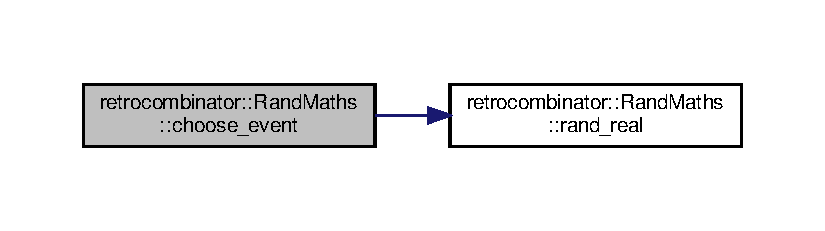
\includegraphics[width=350pt]{classretrocombinator_1_1RandMaths_a3834f9a074546f0d588247610f16fb0e_cgraph}
\end{center}
\end{figure}
Here is the caller graph for this function\+:\nopagebreak
\begin{figure}[H]
\begin{center}
\leavevmode
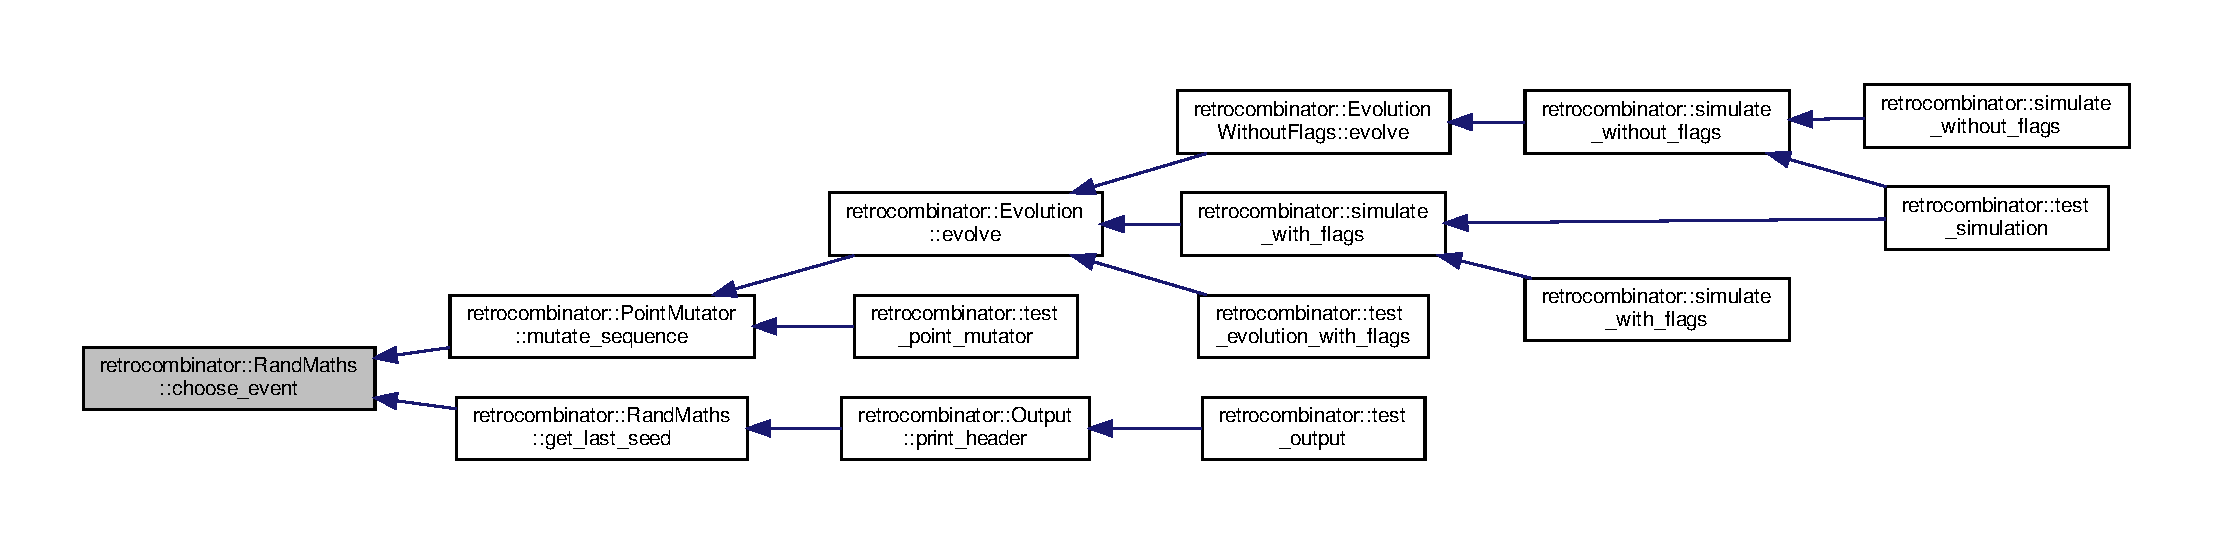
\includegraphics[width=350pt]{classretrocombinator_1_1RandMaths_a3834f9a074546f0d588247610f16fb0e_icgraph}
\end{center}
\end{figure}
\mbox{\Hypertarget{classretrocombinator_1_1RandMaths_a801f694872b80cd801824d8984f7825a}\label{classretrocombinator_1_1RandMaths_a801f694872b80cd801824d8984f7825a}} 
\index{retrocombinator::RandMaths@{retrocombinator::RandMaths}!choose\_event@{choose\_event}}
\index{choose\_event@{choose\_event}!retrocombinator::RandMaths@{retrocombinator::RandMaths}}
\doxysubsubsection{\texorpdfstring{choose\_event()}{choose\_event()}\hspace{0.1cm}{\footnotesize\ttfamily [2/2]}}
{\footnotesize\ttfamily template$<$typename T $>$ \\
\mbox{\hyperlink{namespaceretrocombinator_a8e1541b50cee66a791df4c437ccbb385}{size\+\_\+type}} retrocombinator\+::\+Rand\+Maths\+::choose\+\_\+event (\begin{DoxyParamCaption}\item[{const std\+::vector$<$ T $>$}]{events }\end{DoxyParamCaption})\hspace{0.3cm}{\ttfamily [inline]}}



Chooses an event from a list of possible events. 

Takes the {\itshape relative} probabilities of each of the events as input Here is the call graph for this function\+:\nopagebreak
\begin{figure}[H]
\begin{center}
\leavevmode
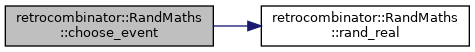
\includegraphics[width=350pt]{classretrocombinator_1_1RandMaths_a801f694872b80cd801824d8984f7825a_cgraph}
\end{center}
\end{figure}
\mbox{\Hypertarget{classretrocombinator_1_1RandMaths_a119bf0b2c75779517d0dabf58c8169bb}\label{classretrocombinator_1_1RandMaths_a119bf0b2c75779517d0dabf58c8169bb}} 
\index{retrocombinator::RandMaths@{retrocombinator::RandMaths}!choose\_events@{choose\_events}}
\index{choose\_events@{choose\_events}!retrocombinator::RandMaths@{retrocombinator::RandMaths}}
\doxysubsubsection{\texorpdfstring{choose\_events()}{choose\_events()}}
{\footnotesize\ttfamily template$<$typename T $>$ \\
std\+::vector$<$\mbox{\hyperlink{namespaceretrocombinator_a8e1541b50cee66a791df4c437ccbb385}{size\+\_\+type}}$>$ retrocombinator\+::\+Rand\+Maths\+::choose\+\_\+events (\begin{DoxyParamCaption}\item[{std\+::vector$<$ T $>$}]{events,  }\item[{\mbox{\hyperlink{namespaceretrocombinator_a8e1541b50cee66a791df4c437ccbb385}{size\+\_\+type}}}]{num\+\_\+picks }\end{DoxyParamCaption})\hspace{0.3cm}{\ttfamily [inline]}}



Chooses many events from a list of possible events, with replacement. 

Returns a vector {\ttfamily picks} of the same size as events, where {\itshape picks\+\_\+i} is the number of times event {\ttfamily i} was chosen.

Takes the {\itshape relative} probabilities of each of the events as input. Here is the call graph for this function\+:\nopagebreak
\begin{figure}[H]
\begin{center}
\leavevmode
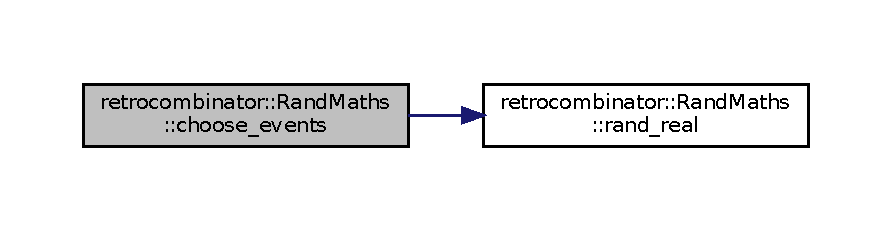
\includegraphics[width=350pt]{classretrocombinator_1_1RandMaths_a119bf0b2c75779517d0dabf58c8169bb_cgraph}
\end{center}
\end{figure}
\mbox{\Hypertarget{classretrocombinator_1_1RandMaths_a2d4fdd627a0d5e24da1d8affec21ac28}\label{classretrocombinator_1_1RandMaths_a2d4fdd627a0d5e24da1d8affec21ac28}} 
\index{retrocombinator::RandMaths@{retrocombinator::RandMaths}!choose\_items@{choose\_items}}
\index{choose\_items@{choose\_items}!retrocombinator::RandMaths@{retrocombinator::RandMaths}}
\doxysubsubsection{\texorpdfstring{choose\_items()}{choose\_items()}}
{\footnotesize\ttfamily std\+::vector$<$ \mbox{\hyperlink{namespaceretrocombinator_a8e1541b50cee66a791df4c437ccbb385}{size\+\_\+type}} $>$ Rand\+Maths\+::choose\+\_\+items (\begin{DoxyParamCaption}\item[{std\+::vector$<$ \mbox{\hyperlink{namespaceretrocombinator_a8e1541b50cee66a791df4c437ccbb385}{size\+\_\+type}} $>$}]{items,  }\item[{\mbox{\hyperlink{namespaceretrocombinator_a8e1541b50cee66a791df4c437ccbb385}{size\+\_\+type}}}]{num\+\_\+picks }\end{DoxyParamCaption})}



Chooses (without replacement) a given number of items randomly from a list of distinct types, where each type has some number of items to begin with. 

Returns a vector {\ttfamily picks} of the same size as items, where {\itshape picks\+\_\+i} is the number of times item {\itshape i} was chosen, and {\itshape picks\+\_\+i} $<$= {\ttfamily item\+\_\+i} 

If the number of items to be picked is larger than we have available, all items are picked and so we just return the original list given to us. Here is the caller graph for this function\+:\nopagebreak
\begin{figure}[H]
\begin{center}
\leavevmode
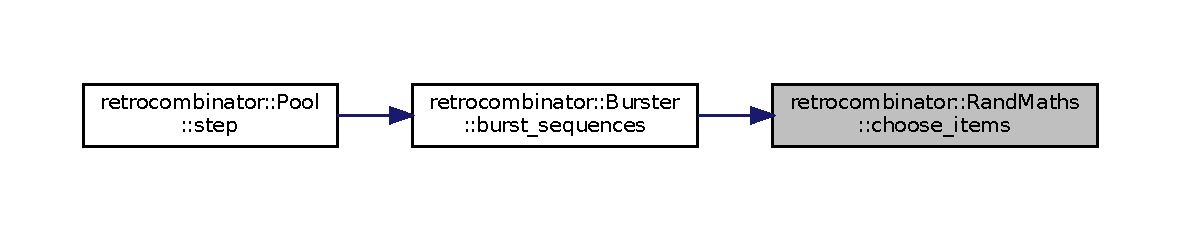
\includegraphics[width=350pt]{classretrocombinator_1_1RandMaths_a2d4fdd627a0d5e24da1d8affec21ac28_icgraph}
\end{center}
\end{figure}
\mbox{\Hypertarget{classretrocombinator_1_1RandMaths_ae54dee1a16fb0e275e1624ccaa7dc87e}\label{classretrocombinator_1_1RandMaths_ae54dee1a16fb0e275e1624ccaa7dc87e}} 
\index{retrocombinator::RandMaths@{retrocombinator::RandMaths}!get\_instance@{get\_instance}}
\index{get\_instance@{get\_instance}!retrocombinator::RandMaths@{retrocombinator::RandMaths}}
\doxysubsubsection{\texorpdfstring{get\_instance()}{get\_instance()}}
{\footnotesize\ttfamily \mbox{\hyperlink{classretrocombinator_1_1RandMaths}{Rand\+Maths}} \& Rand\+Maths\+::get\+\_\+instance (\begin{DoxyParamCaption}{ }\end{DoxyParamCaption})\hspace{0.3cm}{\ttfamily [static]}}



Returns an instance of a \mbox{\hyperlink{classretrocombinator_1_1RandMaths}{Rand\+Maths}} class, after seeding it with system time. 

Can be done only once as we want to share the random number generation among all other classes, and seed only once for controlling the numbers that are generated. \mbox{\Hypertarget{classretrocombinator_1_1RandMaths_a59d3ee4c79f732e3f0b9e587bd4f66e9}\label{classretrocombinator_1_1RandMaths_a59d3ee4c79f732e3f0b9e587bd4f66e9}} 
\index{retrocombinator::RandMaths@{retrocombinator::RandMaths}!get\_last\_seed@{get\_last\_seed}}
\index{get\_last\_seed@{get\_last\_seed}!retrocombinator::RandMaths@{retrocombinator::RandMaths}}
\doxysubsubsection{\texorpdfstring{get\_last\_seed()}{get\_last\_seed()}}
{\footnotesize\ttfamily \mbox{\hyperlink{namespaceretrocombinator_a8e1541b50cee66a791df4c437ccbb385}{size\+\_\+type}} retrocombinator\+::\+Rand\+Maths\+::get\+\_\+last\+\_\+seed (\begin{DoxyParamCaption}{ }\end{DoxyParamCaption}) const\hspace{0.3cm}{\ttfamily [inline]}}



Gets the last set seed. 

Look at the definition of last\+\_\+seed for more details. \mbox{\Hypertarget{classretrocombinator_1_1RandMaths_a8072bad64e64ef042e5257e1bee85635}\label{classretrocombinator_1_1RandMaths_a8072bad64e64ef042e5257e1bee85635}} 
\index{retrocombinator::RandMaths@{retrocombinator::RandMaths}!rand\_int@{rand\_int}}
\index{rand\_int@{rand\_int}!retrocombinator::RandMaths@{retrocombinator::RandMaths}}
\doxysubsubsection{\texorpdfstring{rand\_int()}{rand\_int()}}
{\footnotesize\ttfamily \mbox{\hyperlink{namespaceretrocombinator_a8e1541b50cee66a791df4c437ccbb385}{size\+\_\+type}} Rand\+Maths\+::rand\+\_\+int (\begin{DoxyParamCaption}\item[{\mbox{\hyperlink{namespaceretrocombinator_a8e1541b50cee66a791df4c437ccbb385}{size\+\_\+type}}}]{low,  }\item[{\mbox{\hyperlink{namespaceretrocombinator_a8e1541b50cee66a791df4c437ccbb385}{size\+\_\+type}}}]{high }\end{DoxyParamCaption})}



Generates a random integer within a range. 

The bounds are \mbox{[}inclusive\+\_\+low, exclusive\+\_\+high). Here is the caller graph for this function\+:\nopagebreak
\begin{figure}[H]
\begin{center}
\leavevmode
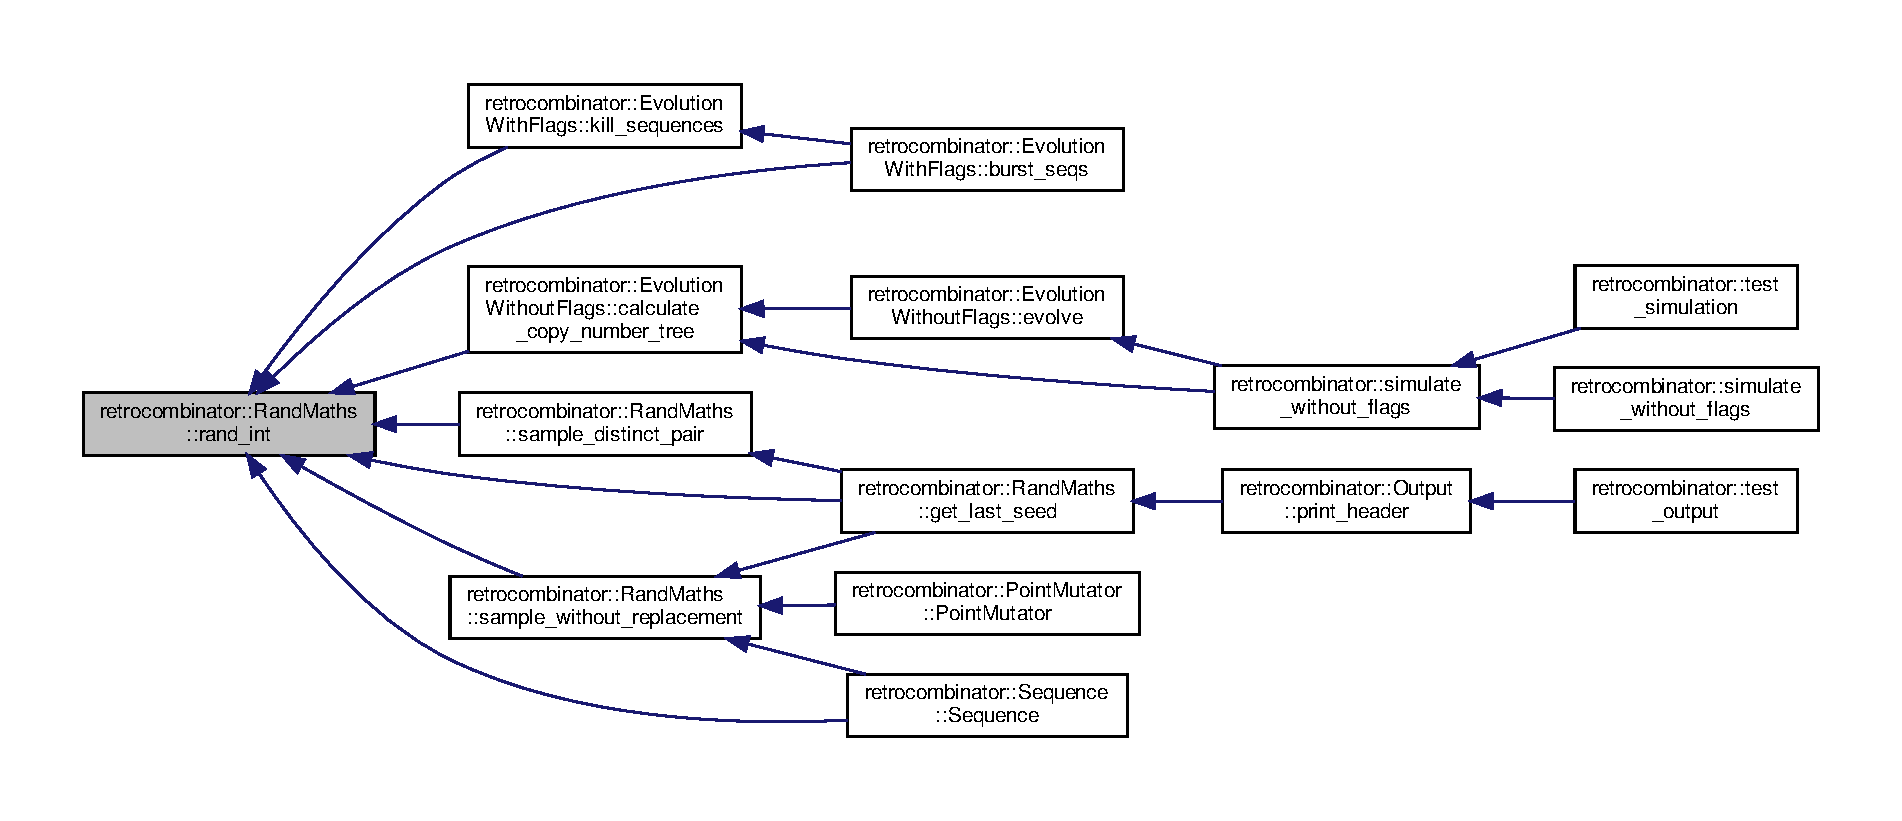
\includegraphics[width=350pt]{classretrocombinator_1_1RandMaths_a8072bad64e64ef042e5257e1bee85635_icgraph}
\end{center}
\end{figure}
\mbox{\Hypertarget{classretrocombinator_1_1RandMaths_adef66efd4d58f6130982ff0ee0e25750}\label{classretrocombinator_1_1RandMaths_adef66efd4d58f6130982ff0ee0e25750}} 
\index{retrocombinator::RandMaths@{retrocombinator::RandMaths}!rand\_poisson@{rand\_poisson}}
\index{rand\_poisson@{rand\_poisson}!retrocombinator::RandMaths@{retrocombinator::RandMaths}}
\doxysubsubsection{\texorpdfstring{rand\_poisson()}{rand\_poisson()}}
{\footnotesize\ttfamily \mbox{\hyperlink{namespaceretrocombinator_a8e1541b50cee66a791df4c437ccbb385}{size\+\_\+type}} Rand\+Maths\+::rand\+\_\+poisson (\begin{DoxyParamCaption}\item[{double}]{mean }\end{DoxyParamCaption})}



Chooses a number sampled from a Poisson distribution. 

Takes the mean as a parameter. Here is the caller graph for this function\+:\nopagebreak
\begin{figure}[H]
\begin{center}
\leavevmode
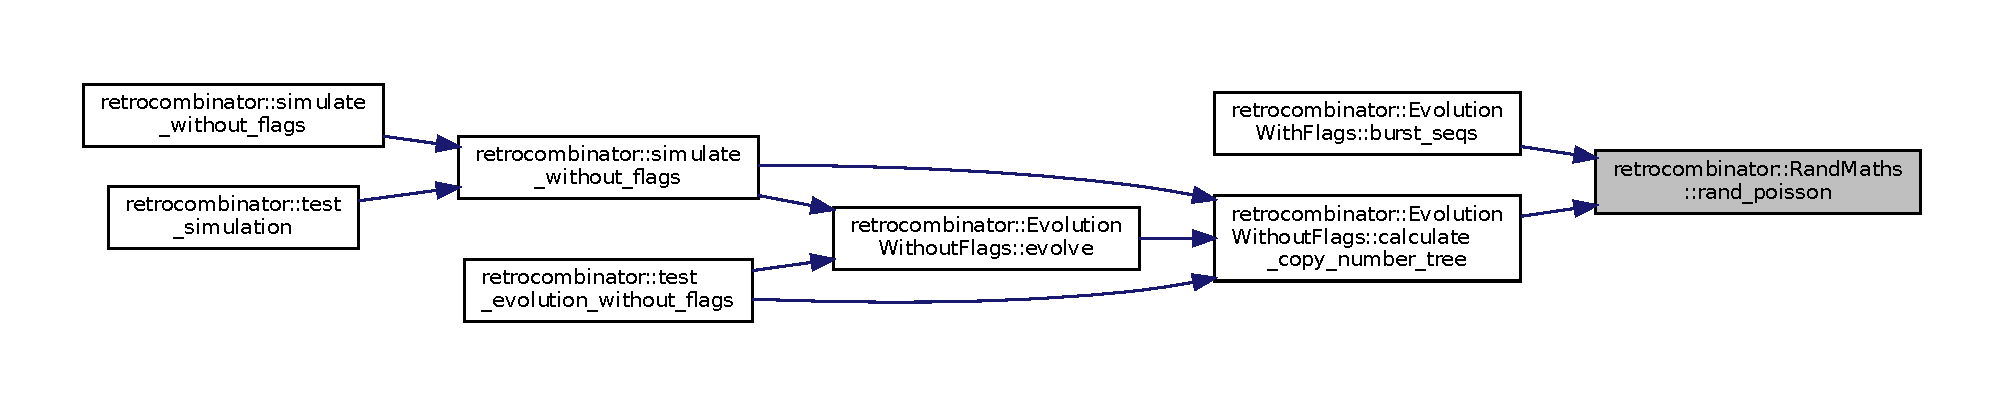
\includegraphics[width=350pt]{classretrocombinator_1_1RandMaths_adef66efd4d58f6130982ff0ee0e25750_icgraph}
\end{center}
\end{figure}
\mbox{\Hypertarget{classretrocombinator_1_1RandMaths_aa6441baa59bff50f588c0c54e3c54140}\label{classretrocombinator_1_1RandMaths_aa6441baa59bff50f588c0c54e3c54140}} 
\index{retrocombinator::RandMaths@{retrocombinator::RandMaths}!rand\_real@{rand\_real}}
\index{rand\_real@{rand\_real}!retrocombinator::RandMaths@{retrocombinator::RandMaths}}
\doxysubsubsection{\texorpdfstring{rand\_real()}{rand\_real()}}
{\footnotesize\ttfamily double Rand\+Maths\+::rand\+\_\+real (\begin{DoxyParamCaption}\item[{double}]{low = {\ttfamily 0.0},  }\item[{double}]{high = {\ttfamily 1.0} }\end{DoxyParamCaption})}



Generates a random real number within a range. 

The bounds are \mbox{[}inclusive\+\_\+low, exclusive high). Here is the caller graph for this function\+:\nopagebreak
\begin{figure}[H]
\begin{center}
\leavevmode
\includegraphics[width=350pt]{classretrocombinator_1_1RandMaths_aa6441baa59bff50f588c0c54e3c54140_icgraph}
\end{center}
\end{figure}
\mbox{\Hypertarget{classretrocombinator_1_1RandMaths_a2758ba7c9818bc664c4b751a697e1fe6}\label{classretrocombinator_1_1RandMaths_a2758ba7c9818bc664c4b751a697e1fe6}} 
\index{retrocombinator::RandMaths@{retrocombinator::RandMaths}!sample\_distinct\_pair@{sample\_distinct\_pair}}
\index{sample\_distinct\_pair@{sample\_distinct\_pair}!retrocombinator::RandMaths@{retrocombinator::RandMaths}}
\doxysubsubsection{\texorpdfstring{sample\_distinct\_pair()}{sample\_distinct\_pair()}}
{\footnotesize\ttfamily std\+::pair$<$ \mbox{\hyperlink{namespaceretrocombinator_a8e1541b50cee66a791df4c437ccbb385}{size\+\_\+type}}, \mbox{\hyperlink{namespaceretrocombinator_a8e1541b50cee66a791df4c437ccbb385}{size\+\_\+type}} $>$ Rand\+Maths\+::sample\+\_\+distinct\+\_\+pair (\begin{DoxyParamCaption}\item[{\mbox{\hyperlink{namespaceretrocombinator_a8e1541b50cee66a791df4c437ccbb385}{size\+\_\+type}}}]{low,  }\item[{\mbox{\hyperlink{namespaceretrocombinator_a8e1541b50cee66a791df4c437ccbb385}{size\+\_\+type}}}]{high }\end{DoxyParamCaption})}



Samples a non-\/diagonal pair (2 distinct values) within a range. 

The bounds for each value are \mbox{[}inclusive\+\_\+low, exclusive high). Here is the call graph for this function\+:\nopagebreak
\begin{figure}[H]
\begin{center}
\leavevmode
\includegraphics[width=350pt]{classretrocombinator_1_1RandMaths_a2758ba7c9818bc664c4b751a697e1fe6_cgraph}
\end{center}
\end{figure}
\mbox{\Hypertarget{classretrocombinator_1_1RandMaths_a6a7fe159f46afec51d997e4d07d2cfe6}\label{classretrocombinator_1_1RandMaths_a6a7fe159f46afec51d997e4d07d2cfe6}} 
\index{retrocombinator::RandMaths@{retrocombinator::RandMaths}!sample\_without\_replacement@{sample\_without\_replacement}}
\index{sample\_without\_replacement@{sample\_without\_replacement}!retrocombinator::RandMaths@{retrocombinator::RandMaths}}
\doxysubsubsection{\texorpdfstring{sample\_without\_replacement()}{sample\_without\_replacement()}}
{\footnotesize\ttfamily std\+::set$<$ \mbox{\hyperlink{namespaceretrocombinator_a8e1541b50cee66a791df4c437ccbb385}{size\+\_\+type}} $>$ Rand\+Maths\+::sample\+\_\+without\+\_\+replacement (\begin{DoxyParamCaption}\item[{\mbox{\hyperlink{namespaceretrocombinator_a8e1541b50cee66a791df4c437ccbb385}{size\+\_\+type}}}]{low,  }\item[{\mbox{\hyperlink{namespaceretrocombinator_a8e1541b50cee66a791df4c437ccbb385}{size\+\_\+type}}}]{high,  }\item[{\mbox{\hyperlink{namespaceretrocombinator_a8e1541b50cee66a791df4c437ccbb385}{size\+\_\+type}}}]{m }\end{DoxyParamCaption})}



Samples {\itshape m} integers within a range, without replacement. 

The bounds are \mbox{[}inclusive\+\_\+low, exclusive high). The integers are returned in ascending order. Here is the call graph for this function\+:\nopagebreak
\begin{figure}[H]
\begin{center}
\leavevmode
\includegraphics[width=350pt]{classretrocombinator_1_1RandMaths_a6a7fe159f46afec51d997e4d07d2cfe6_cgraph}
\end{center}
\end{figure}
Here is the caller graph for this function\+:\nopagebreak
\begin{figure}[H]
\begin{center}
\leavevmode
\includegraphics[width=350pt]{classretrocombinator_1_1RandMaths_a6a7fe159f46afec51d997e4d07d2cfe6_icgraph}
\end{center}
\end{figure}
\mbox{\Hypertarget{classretrocombinator_1_1RandMaths_a2b61e31de6067ffa35531d5bde40f4c6}\label{classretrocombinator_1_1RandMaths_a2b61e31de6067ffa35531d5bde40f4c6}} 
\index{retrocombinator::RandMaths@{retrocombinator::RandMaths}!set\_random\_seed@{set\_random\_seed}}
\index{set\_random\_seed@{set\_random\_seed}!retrocombinator::RandMaths@{retrocombinator::RandMaths}}
\doxysubsubsection{\texorpdfstring{set\_random\_seed()}{set\_random\_seed()}}
{\footnotesize\ttfamily void Rand\+Maths\+::set\+\_\+random\+\_\+seed (\begin{DoxyParamCaption}{ }\end{DoxyParamCaption})}



Uses system time to seed the R\+NG. 

This can be undone by calling {\ttfamily \mbox{\hyperlink{classretrocombinator_1_1RandMaths_a0bf1c2e7a1eccb1f9246b3fceeb5db8a}{set\+\_\+specific\+\_\+seed()}}} \mbox{\Hypertarget{classretrocombinator_1_1RandMaths_a0bf1c2e7a1eccb1f9246b3fceeb5db8a}\label{classretrocombinator_1_1RandMaths_a0bf1c2e7a1eccb1f9246b3fceeb5db8a}} 
\index{retrocombinator::RandMaths@{retrocombinator::RandMaths}!set\_specific\_seed@{set\_specific\_seed}}
\index{set\_specific\_seed@{set\_specific\_seed}!retrocombinator::RandMaths@{retrocombinator::RandMaths}}
\doxysubsubsection{\texorpdfstring{set\_specific\_seed()}{set\_specific\_seed()}}
{\footnotesize\ttfamily void Rand\+Maths\+::set\+\_\+specific\+\_\+seed (\begin{DoxyParamCaption}\item[{\mbox{\hyperlink{namespaceretrocombinator_a8e1541b50cee66a791df4c437ccbb385}{size\+\_\+type}}}]{seed }\end{DoxyParamCaption})}



Uses a user-\/specified seed for R\+NG. 

This can be undone by calling {\ttfamily \mbox{\hyperlink{classretrocombinator_1_1RandMaths_a2b61e31de6067ffa35531d5bde40f4c6}{set\+\_\+random\+\_\+seed()}}} \mbox{\Hypertarget{classretrocombinator_1_1RandMaths_a183686140a9da18ad40c7e048ee8914e}\label{classretrocombinator_1_1RandMaths_a183686140a9da18ad40c7e048ee8914e}} 
\index{retrocombinator::RandMaths@{retrocombinator::RandMaths}!test\_event@{test\_event}}
\index{test\_event@{test\_event}!retrocombinator::RandMaths@{retrocombinator::RandMaths}}
\doxysubsubsection{\texorpdfstring{test\_event()}{test\_event()}}
{\footnotesize\ttfamily bool Rand\+Maths\+::test\+\_\+event (\begin{DoxyParamCaption}\item[{double}]{event\+\_\+probability }\end{DoxyParamCaption})}



Tests whether or not an event happened. 

Takes the probability of an event as parameter, and then compares it to a random value in \mbox{[}0, 1). Here is the call graph for this function\+:\nopagebreak
\begin{figure}[H]
\begin{center}
\leavevmode
\includegraphics[width=350pt]{classretrocombinator_1_1RandMaths_a183686140a9da18ad40c7e048ee8914e_cgraph}
\end{center}
\end{figure}
Here is the caller graph for this function\+:\nopagebreak
\begin{figure}[H]
\begin{center}
\leavevmode
\includegraphics[width=350pt]{classretrocombinator_1_1RandMaths_a183686140a9da18ad40c7e048ee8914e_icgraph}
\end{center}
\end{figure}


\doxysubsection{Member Data Documentation}
\mbox{\Hypertarget{classretrocombinator_1_1RandMaths_ab5b6bec8e0eaea80efe565cddc8e69ac}\label{classretrocombinator_1_1RandMaths_ab5b6bec8e0eaea80efe565cddc8e69ac}} 
\index{retrocombinator::RandMaths@{retrocombinator::RandMaths}!last\_seed@{last\_seed}}
\index{last\_seed@{last\_seed}!retrocombinator::RandMaths@{retrocombinator::RandMaths}}
\doxysubsubsection{\texorpdfstring{last\_seed}{last\_seed}}
{\footnotesize\ttfamily \mbox{\hyperlink{namespaceretrocombinator_a8e1541b50cee66a791df4c437ccbb385}{size\+\_\+type}} retrocombinator\+::\+Rand\+Maths\+::last\+\_\+seed\hspace{0.3cm}{\ttfamily [private]}}



Last seed for the random engine, either by the user or by the system. 

Note that this does not reflect the internal state of the random engine at all points as once random number generation begins, this value is not touched. \mbox{\Hypertarget{classretrocombinator_1_1RandMaths_a8455f3a94efd124edd0ecfc806744476}\label{classretrocombinator_1_1RandMaths_a8455f3a94efd124edd0ecfc806744476}} 
\index{retrocombinator::RandMaths@{retrocombinator::RandMaths}!re@{re}}
\index{re@{re}!retrocombinator::RandMaths@{retrocombinator::RandMaths}}
\doxysubsubsection{\texorpdfstring{re}{re}}
{\footnotesize\ttfamily std\+::mt19937 retrocombinator\+::\+Rand\+Maths\+::re\hspace{0.3cm}{\ttfamily [private]}}



Engine that produces random numbers for all functions that require them. 

This is seeded during initialisation of the class, and once set, its R\+NG is shared by all other parts of the code that require it. 

The documentation for this class was generated from the following files\+:\begin{DoxyCompactItemize}
\item 
src/\mbox{\hyperlink{rand__maths_8h}{rand\+\_\+maths.\+h}}\item 
src/rand\+\_\+maths.\+cpp\end{DoxyCompactItemize}

\hypertarget{classretrocombinator_1_1Sequence}{}\section{retrocombinator\+:\+:Sequence Class Reference}
\label{classretrocombinator_1_1Sequence}\index{retrocombinator\+::\+Sequence@{retrocombinator\+::\+Sequence}}


To represent a D\+NA sequence and the mutations that it has undergone.  




{\ttfamily \#include $<$sequence.\+h$>$}

\subsection*{Public Member Functions}
\begin{DoxyCompactItemize}
\item 
\hyperlink{classretrocombinator_1_1Sequence_a04d0d6977316f2ab30844e584c4531ec}{Sequence} (\hyperlink{namespaceretrocombinator_a8e1541b50cee66a791df4c437ccbb385}{size\+\_\+type} n)
\begin{DoxyCompactList}\small\item\em Constructs a random sequence of length {\itshape n}. \end{DoxyCompactList}\item 
\hyperlink{classretrocombinator_1_1Sequence_af5b3b62eba07f0e09f532fcf1681c289}{Sequence} (std\+::string s)
\begin{DoxyCompactList}\small\item\em Constructs a sequence from a given string. \end{DoxyCompactList}\item 
\hyperlink{classretrocombinator_1_1Sequence_af334c44bea806196b5037e61b0e831b1}{Sequence} (const \hyperlink{classretrocombinator_1_1Sequence}{Sequence} \&s1, const \hyperlink{classretrocombinator_1_1Sequence}{Sequence} \&s2, \hyperlink{namespaceretrocombinator_a8e1541b50cee66a791df4c437ccbb385}{size\+\_\+type} num\+\_\+template\+\_\+switches)
\begin{DoxyCompactList}\small\item\em Constructs a sequence from recombining two other sequences. \end{DoxyCompactList}\item 
\mbox{\Hypertarget{classretrocombinator_1_1Sequence_aeefc98943c08769af4ed9f73157d26d1}\label{classretrocombinator_1_1Sequence_aeefc98943c08769af4ed9f73157d26d1}} 
\hyperlink{namespaceretrocombinator_a8e1541b50cee66a791df4c437ccbb385}{size\+\_\+type} \hyperlink{classretrocombinator_1_1Sequence_aeefc98943c08769af4ed9f73157d26d1}{get\+\_\+length} () const
\begin{DoxyCompactList}\small\item\em Returns length of the sequence. \end{DoxyCompactList}\item 
\mbox{\Hypertarget{classretrocombinator_1_1Sequence_a6ef8ac65b574f4c0d6155b67efe581ec}\label{classretrocombinator_1_1Sequence_a6ef8ac65b574f4c0d6155b67efe581ec}} 
\hyperlink{namespaceretrocombinator_afd7c6eb4293e8c4d12827609a9a34b9b}{tag\+\_\+type} \hyperlink{classretrocombinator_1_1Sequence_a6ef8ac65b574f4c0d6155b67efe581ec}{get\+\_\+tag} () const
\begin{DoxyCompactList}\small\item\em Returns the unique label for this sequence. \end{DoxyCompactList}\item 
std\+::pair$<$ \hyperlink{namespaceretrocombinator_afd7c6eb4293e8c4d12827609a9a34b9b}{tag\+\_\+type}, \hyperlink{namespaceretrocombinator_afd7c6eb4293e8c4d12827609a9a34b9b}{tag\+\_\+type} $>$ \hyperlink{classretrocombinator_1_1Sequence_abd985b5164277d63c40f9580882335c8}{get\+\_\+parent\+\_\+tags} () const
\begin{DoxyCompactList}\small\item\em Returns the tags of the sequences that this sequence was created from. \end{DoxyCompactList}\item 
\mbox{\Hypertarget{classretrocombinator_1_1Sequence_a23c73a4ccfbe9baded2e99479e3ffb5e}\label{classretrocombinator_1_1Sequence_a23c73a4ccfbe9baded2e99479e3ffb5e}} 
char \hyperlink{classretrocombinator_1_1Sequence_a23c73a4ccfbe9baded2e99479e3ffb5e}{char\+\_\+at} (\hyperlink{namespaceretrocombinator_a8e1541b50cee66a791df4c437ccbb385}{size\+\_\+type} n) const
\begin{DoxyCompactList}\small\item\em Returns the character for a base at a given position. \end{DoxyCompactList}\item 
void \hyperlink{classretrocombinator_1_1Sequence_a85299c3dbf2efb993a43acc2e42fcb00}{point\+\_\+mutate} (\hyperlink{namespaceretrocombinator_a8e1541b50cee66a791df4c437ccbb385}{size\+\_\+type} n, char new\+\_\+nucleotide, bool is\+\_\+lethal=false)
\begin{DoxyCompactList}\small\item\em Changes the nucleotide at position {\itshape n} to {\itshape new\+\_\+nucleotide}. \end{DoxyCompactList}\item 
\mbox{\Hypertarget{classretrocombinator_1_1Sequence_a5fa45e155a1e4b3c257f19369ace05a8}\label{classretrocombinator_1_1Sequence_a5fa45e155a1e4b3c257f19369ace05a8}} 
std\+::string \hyperlink{classretrocombinator_1_1Sequence_a5fa45e155a1e4b3c257f19369ace05a8}{as\+\_\+string} () const
\begin{DoxyCompactList}\small\item\em Returns the raw nucleotide sequence as a string. \end{DoxyCompactList}\item 
bool \hyperlink{classretrocombinator_1_1Sequence_a445120376c2e5c626d3ecfa509406843}{is\+\_\+active} () const
\begin{DoxyCompactList}\small\item\em Tests whether this sequence is active (can transpose) or not. \end{DoxyCompactList}\item 
\mbox{\Hypertarget{classretrocombinator_1_1Sequence_a1140bea4ad0375ee514d140aa80e9bd5}\label{classretrocombinator_1_1Sequence_a1140bea4ad0375ee514d140aa80e9bd5}} 
\hyperlink{namespaceretrocombinator_a8e1541b50cee66a791df4c437ccbb385}{size\+\_\+type} \hyperlink{classretrocombinator_1_1Sequence_a1140bea4ad0375ee514d140aa80e9bd5}{num\+\_\+mutations} () const
\begin{DoxyCompactList}\small\item\em Returns how many mutations are present in this sequence. \end{DoxyCompactList}\item 
\mbox{\Hypertarget{classretrocombinator_1_1Sequence_aaac564e24289e894507c99b82946f492}\label{classretrocombinator_1_1Sequence_aaac564e24289e894507c99b82946f492}} 
double \hyperlink{classretrocombinator_1_1Sequence_aaac564e24289e894507c99b82946f492}{init\+\_\+seq\+\_\+similarity} () const
\begin{DoxyCompactList}\small\item\em Returns sequence similarity to initial sequence. \end{DoxyCompactList}\end{DoxyCompactItemize}
\textbf{ }\par
\begin{DoxyCompactItemize}
\item 
\mbox{\Hypertarget{classretrocombinator_1_1Sequence_a5cf77ea0b07ba519d1f79ea781a77e8a}\label{classretrocombinator_1_1Sequence_a5cf77ea0b07ba519d1f79ea781a77e8a}} 
\hyperlink{classretrocombinator_1_1Sequence_a5cf77ea0b07ba519d1f79ea781a77e8a}{Sequence} (\hyperlink{classretrocombinator_1_1Sequence}{Sequence} const \&)=delete
\begin{DoxyCompactList}\small\item\em Delete copy constructors as we want tags to be unique. \end{DoxyCompactList}\item 
\mbox{\Hypertarget{classretrocombinator_1_1Sequence_aca2b4e5813b22d5181883c3de069301e}\label{classretrocombinator_1_1Sequence_aca2b4e5813b22d5181883c3de069301e}} 
void {\bfseries operator=} (\hyperlink{classretrocombinator_1_1Sequence}{Sequence} const \&)=delete
\end{DoxyCompactItemize}

\textbf{ }\par
\begin{DoxyCompactItemize}
\item 
\mbox{\Hypertarget{classretrocombinator_1_1Sequence_aa7350870199cd599d0345bbc563ec239}\label{classretrocombinator_1_1Sequence_aa7350870199cd599d0345bbc563ec239}} 
\hyperlink{classretrocombinator_1_1Sequence_aa7350870199cd599d0345bbc563ec239}{Sequence} (\hyperlink{classretrocombinator_1_1Sequence}{Sequence} \&\&)=default
\begin{DoxyCompactList}\small\item\em But make the objects moveable, to create containers of them. \end{DoxyCompactList}\item 
\mbox{\Hypertarget{classretrocombinator_1_1Sequence_a3f08f9281e5b350ed824f857a78c1647}\label{classretrocombinator_1_1Sequence_a3f08f9281e5b350ed824f857a78c1647}} 
\hyperlink{classretrocombinator_1_1Sequence}{Sequence} \& {\bfseries operator=} (\hyperlink{classretrocombinator_1_1Sequence}{Sequence} \&\&)=default
\end{DoxyCompactItemize}

\subsection*{Static Public Member Functions}
\begin{DoxyCompactItemize}
\item 
static void \hyperlink{classretrocombinator_1_1Sequence_ad4791ec3cefbea417081cd349ac6c23b}{renumber\+\_\+sequences} (\hyperlink{namespaceretrocombinator_afd7c6eb4293e8c4d12827609a9a34b9b}{tag\+\_\+type} new\+\_\+start\+\_\+tag)
\begin{DoxyCompactList}\small\item\em Explicitly update the global sequence count to start from a particular number. \end{DoxyCompactList}\end{DoxyCompactItemize}
\subsection*{Static Public Attributes}
\textbf{ }\par
\begin{DoxyCompactItemize}
\item 
\mbox{\Hypertarget{classretrocombinator_1_1Sequence_aa89fde879519ff0513fce29a4d0a554a}\label{classretrocombinator_1_1Sequence_aa89fde879519ff0513fce29a4d0a554a}} 
static const \hyperlink{namespaceretrocombinator_afd7c6eb4293e8c4d12827609a9a34b9b}{tag\+\_\+type} \hyperlink{classretrocombinator_1_1Sequence_aa89fde879519ff0513fce29a4d0a554a}{R\+A\+ND} = -\/10
\begin{DoxyCompactList}\small\item\em This sequence was created randomly. \end{DoxyCompactList}\item 
\mbox{\Hypertarget{classretrocombinator_1_1Sequence_a3ded5ce523bc4ed7471f33dda1ffa8c3}\label{classretrocombinator_1_1Sequence_a3ded5ce523bc4ed7471f33dda1ffa8c3}} 
static const \hyperlink{namespaceretrocombinator_afd7c6eb4293e8c4d12827609a9a34b9b}{tag\+\_\+type} \hyperlink{classretrocombinator_1_1Sequence_a3ded5ce523bc4ed7471f33dda1ffa8c3}{I\+N\+IT} = -\/20
\begin{DoxyCompactList}\small\item\em This sequence was created from a specified string. \end{DoxyCompactList}\end{DoxyCompactItemize}

\subsection*{Private Types}
\textbf{ }\par
\begin{DoxyCompactItemize}
\item 
typedef std\+::unordered\+\_\+map$<$ \hyperlink{namespaceretrocombinator_afd7c6eb4293e8c4d12827609a9a34b9b}{tag\+\_\+type}, char $>$ \hyperlink{classretrocombinator_1_1Sequence_a2abbaf2376f035a997e02c4afae9f476}{mutations\+\_\+type}
\begin{DoxyCompactList}\small\item\em Basic typedefs -\/ hashed data structures for quick lookup. \end{DoxyCompactList}\item 
\mbox{\Hypertarget{classretrocombinator_1_1Sequence_aabef8f6c5b05d1343705872e8d17368f}\label{classretrocombinator_1_1Sequence_aabef8f6c5b05d1343705872e8d17368f}} 
typedef std\+::unordered\+\_\+set$<$ \hyperlink{namespaceretrocombinator_afd7c6eb4293e8c4d12827609a9a34b9b}{tag\+\_\+type} $>$ {\bfseries lethal\+\_\+mutations\+\_\+type}
\end{DoxyCompactItemize}

\subsection*{Private Member Functions}
\begin{DoxyCompactItemize}
\item 
\mbox{\Hypertarget{classretrocombinator_1_1Sequence_a378e5aecc7fa4524cd90d352cfd651fe}\label{classretrocombinator_1_1Sequence_a378e5aecc7fa4524cd90d352cfd651fe}} 
std\+::pair$<$ bool, bool $>$ \hyperlink{classretrocombinator_1_1Sequence_a378e5aecc7fa4524cd90d352cfd651fe}{bits\+\_\+at} (\hyperlink{namespaceretrocombinator_a8e1541b50cee66a791df4c437ccbb385}{size\+\_\+type} n) const
\begin{DoxyCompactList}\small\item\em Returns the 2bit encoding for a base at a given position. \end{DoxyCompactList}\end{DoxyCompactItemize}
\subsection*{Private Attributes}
\begin{DoxyCompactItemize}
\item 
\hyperlink{namespaceretrocombinator_afd7c6eb4293e8c4d12827609a9a34b9b}{tag\+\_\+type} \hyperlink{classretrocombinator_1_1Sequence_ae599e85a84a78e23d33f6c3085248726}{tag}
\begin{DoxyCompactList}\small\item\em A number that uniquely identifies this sequence. \end{DoxyCompactList}\item 
std\+::pair$<$ \hyperlink{namespaceretrocombinator_afd7c6eb4293e8c4d12827609a9a34b9b}{tag\+\_\+type}, \hyperlink{namespaceretrocombinator_afd7c6eb4293e8c4d12827609a9a34b9b}{tag\+\_\+type} $>$ \hyperlink{classretrocombinator_1_1Sequence_a023fef0801bd63048bf5c7b2442694cc}{parent\+\_\+tags}
\begin{DoxyCompactList}\small\item\em The parent tags that this sequence was created from. \end{DoxyCompactList}\item 
std\+::vector$<$ bool $>$ \hyperlink{classretrocombinator_1_1Sequence_a7c6072eaff9990a0bcaebcfa6287e3e0}{bases}
\begin{DoxyCompactList}\small\item\em Actual sequence of nucleotides. \end{DoxyCompactList}\item 
\hyperlink{classretrocombinator_1_1Sequence_a2abbaf2376f035a997e02c4afae9f476}{mutations\+\_\+type} \hyperlink{classretrocombinator_1_1Sequence_a07dd3101f7838d76300313ecfb97f3fc}{mutations}
\begin{DoxyCompactList}\small\item\em Positions of mutations and what the {\itshape original} nucleotide was. \end{DoxyCompactList}\item 
lethal\+\_\+mutations\+\_\+type \hyperlink{classretrocombinator_1_1Sequence_af5798b014aaeb7573197602dafb98818}{lethal\+\_\+mutations}
\begin{DoxyCompactList}\small\item\em Positions of mutations that are lethal. \end{DoxyCompactList}\end{DoxyCompactItemize}
\subsection*{Static Private Attributes}
\begin{DoxyCompactItemize}
\item 
static \hyperlink{namespaceretrocombinator_afd7c6eb4293e8c4d12827609a9a34b9b}{tag\+\_\+type} \hyperlink{classretrocombinator_1_1Sequence_a486f1b680452f7162ee9a895c2871f92}{global\+\_\+sequence\+\_\+count} = -\/1
\begin{DoxyCompactList}\small\item\em An internal counter that is incremented every time a sequence is created. \end{DoxyCompactList}\end{DoxyCompactItemize}
\subsection*{Friends}
\begin{DoxyCompactItemize}
\item 
\hyperlink{namespaceretrocombinator_a8e1541b50cee66a791df4c437ccbb385}{size\+\_\+type} \hyperlink{classretrocombinator_1_1Sequence_a8cd9dc2cfea97399387e2876ee028c32}{operator$\ast$} (const \hyperlink{classretrocombinator_1_1Sequence}{Sequence} \&s1, const \hyperlink{classretrocombinator_1_1Sequence}{Sequence} \&s2)
\begin{DoxyCompactList}\small\item\em Pairwise distances between two sequences. \end{DoxyCompactList}\item 
\hyperlink{namespaceretrocombinator_a8e1541b50cee66a791df4c437ccbb385}{size\+\_\+type} \hyperlink{classretrocombinator_1_1Sequence_afdd1af7009804b182798c40d25bb1bb5}{operator$\ast$} (const \hyperlink{classretrocombinator_1_1Sequence}{Sequence} \&s1, std\+::string s2)
\begin{DoxyCompactList}\small\item\em Pairwise distances between a sequence and a string. \end{DoxyCompactList}\item 
double \hyperlink{classretrocombinator_1_1Sequence_a951eb38b75bb0b9a808e3a8bc7170a09}{operator\%} (const \hyperlink{classretrocombinator_1_1Sequence}{Sequence} \&s1, const \hyperlink{classretrocombinator_1_1Sequence}{Sequence} \&s2)
\begin{DoxyCompactList}\small\item\em Pairwise dissimilarity (\%) between two sequences. \end{DoxyCompactList}\item 
double \hyperlink{classretrocombinator_1_1Sequence_a56fd21ad6db6a3cb7f7f4b9b5b6c84ea}{operator\%} (const \hyperlink{classretrocombinator_1_1Sequence}{Sequence} \&s1, std\+::string s2)
\begin{DoxyCompactList}\small\item\em Pairwise dissimilarity (\%) between a sequence and a string. \end{DoxyCompactList}\end{DoxyCompactItemize}


\subsection{Detailed Description}
To represent a D\+NA sequence and the mutations that it has undergone. 

Keeps track of the actual sequence, mutations and lethal mutations. 

\subsection{Member Typedef Documentation}
\mbox{\Hypertarget{classretrocombinator_1_1Sequence_a2abbaf2376f035a997e02c4afae9f476}\label{classretrocombinator_1_1Sequence_a2abbaf2376f035a997e02c4afae9f476}} 
\index{retrocombinator\+::\+Sequence@{retrocombinator\+::\+Sequence}!mutations\+\_\+type@{mutations\+\_\+type}}
\index{mutations\+\_\+type@{mutations\+\_\+type}!retrocombinator\+::\+Sequence@{retrocombinator\+::\+Sequence}}
\subsubsection{\texorpdfstring{mutations\+\_\+type}{mutations\_type}}
{\footnotesize\ttfamily typedef std\+::unordered\+\_\+map$<$\hyperlink{namespaceretrocombinator_afd7c6eb4293e8c4d12827609a9a34b9b}{tag\+\_\+type}, char$>$ \hyperlink{classretrocombinator_1_1Sequence_a2abbaf2376f035a997e02c4afae9f476}{retrocombinator\+::\+Sequence\+::mutations\+\_\+type}\hspace{0.3cm}{\ttfamily [private]}}



Basic typedefs -\/ hashed data structures for quick lookup. 

For keeping track of mutations and lethal mutations. 

\subsection{Constructor \& Destructor Documentation}
\mbox{\Hypertarget{classretrocombinator_1_1Sequence_a04d0d6977316f2ab30844e584c4531ec}\label{classretrocombinator_1_1Sequence_a04d0d6977316f2ab30844e584c4531ec}} 
\index{retrocombinator\+::\+Sequence@{retrocombinator\+::\+Sequence}!Sequence@{Sequence}}
\index{Sequence@{Sequence}!retrocombinator\+::\+Sequence@{retrocombinator\+::\+Sequence}}
\subsubsection{\texorpdfstring{Sequence()}{Sequence()}\hspace{0.1cm}{\footnotesize\ttfamily [1/3]}}
{\footnotesize\ttfamily Sequence\+::\+Sequence (\begin{DoxyParamCaption}\item[{\hyperlink{namespaceretrocombinator_a8e1541b50cee66a791df4c437ccbb385}{size\+\_\+type}}]{n }\end{DoxyParamCaption})}



Constructs a random sequence of length {\itshape n}. 

This is considered initial, so no mutations are present. Here is the call graph for this function\+:\nopagebreak
\begin{figure}[H]
\begin{center}
\leavevmode
\includegraphics[width=350pt]{classretrocombinator_1_1Sequence_a04d0d6977316f2ab30844e584c4531ec_cgraph}
\end{center}
\end{figure}
\mbox{\Hypertarget{classretrocombinator_1_1Sequence_af5b3b62eba07f0e09f532fcf1681c289}\label{classretrocombinator_1_1Sequence_af5b3b62eba07f0e09f532fcf1681c289}} 
\index{retrocombinator\+::\+Sequence@{retrocombinator\+::\+Sequence}!Sequence@{Sequence}}
\index{Sequence@{Sequence}!retrocombinator\+::\+Sequence@{retrocombinator\+::\+Sequence}}
\subsubsection{\texorpdfstring{Sequence()}{Sequence()}\hspace{0.1cm}{\footnotesize\ttfamily [2/3]}}
{\footnotesize\ttfamily Sequence\+::\+Sequence (\begin{DoxyParamCaption}\item[{std\+::string}]{s }\end{DoxyParamCaption})}



Constructs a sequence from a given string. 

This is considered initial, so no mutations are present. Here is the call graph for this function\+:\nopagebreak
\begin{figure}[H]
\begin{center}
\leavevmode
\includegraphics[width=350pt]{classretrocombinator_1_1Sequence_af5b3b62eba07f0e09f532fcf1681c289_cgraph}
\end{center}
\end{figure}
\mbox{\Hypertarget{classretrocombinator_1_1Sequence_af334c44bea806196b5037e61b0e831b1}\label{classretrocombinator_1_1Sequence_af334c44bea806196b5037e61b0e831b1}} 
\index{retrocombinator\+::\+Sequence@{retrocombinator\+::\+Sequence}!Sequence@{Sequence}}
\index{Sequence@{Sequence}!retrocombinator\+::\+Sequence@{retrocombinator\+::\+Sequence}}
\subsubsection{\texorpdfstring{Sequence()}{Sequence()}\hspace{0.1cm}{\footnotesize\ttfamily [3/3]}}
{\footnotesize\ttfamily Sequence\+::\+Sequence (\begin{DoxyParamCaption}\item[{const \hyperlink{classretrocombinator_1_1Sequence}{Sequence} \&}]{s1,  }\item[{const \hyperlink{classretrocombinator_1_1Sequence}{Sequence} \&}]{s2,  }\item[{\hyperlink{namespaceretrocombinator_a8e1541b50cee66a791df4c437ccbb385}{size\+\_\+type}}]{num\+\_\+template\+\_\+switches }\end{DoxyParamCaption})}



Constructs a sequence from recombining two other sequences. 

The number of template switches has to be specified, and the positions at which the template switches are made is random.

The mutations recorded are with respect to the original sequences. That is, the new sequence {\itshape s\+\_\+new} will have a mutation {\itshape m} at position {\itshape l} if and only if the sequence {\itshape s\+\_\+old} whose nucleotide is used for {\itshape s\+\_\+new} at position {\itshape l} had mutation {\itshape m} present at that position.

\begin{DoxyRefDesc}{Todo}
\item[\hyperlink{todo__todo000001}{Todo}]Add an option for specifying the positions of the template switches too, or overload this function. \end{DoxyRefDesc}
Here is the call graph for this function\+:\nopagebreak
\begin{figure}[H]
\begin{center}
\leavevmode
\includegraphics[width=350pt]{classretrocombinator_1_1Sequence_af334c44bea806196b5037e61b0e831b1_cgraph}
\end{center}
\end{figure}


\subsection{Member Function Documentation}
\mbox{\Hypertarget{classretrocombinator_1_1Sequence_abd985b5164277d63c40f9580882335c8}\label{classretrocombinator_1_1Sequence_abd985b5164277d63c40f9580882335c8}} 
\index{retrocombinator\+::\+Sequence@{retrocombinator\+::\+Sequence}!get\+\_\+parent\+\_\+tags@{get\+\_\+parent\+\_\+tags}}
\index{get\+\_\+parent\+\_\+tags@{get\+\_\+parent\+\_\+tags}!retrocombinator\+::\+Sequence@{retrocombinator\+::\+Sequence}}
\subsubsection{\texorpdfstring{get\+\_\+parent\+\_\+tags()}{get\_parent\_tags()}}
{\footnotesize\ttfamily std\+::pair$<$\hyperlink{namespaceretrocombinator_afd7c6eb4293e8c4d12827609a9a34b9b}{tag\+\_\+type}, \hyperlink{namespaceretrocombinator_afd7c6eb4293e8c4d12827609a9a34b9b}{tag\+\_\+type}$>$ retrocombinator\+::\+Sequence\+::get\+\_\+parent\+\_\+tags (\begin{DoxyParamCaption}{ }\end{DoxyParamCaption}) const\hspace{0.3cm}{\ttfamily [inline]}}



Returns the tags of the sequences that this sequence was created from. 

See the definition of parent\+\_\+tags for more details. Here is the caller graph for this function\+:
\nopagebreak
\begin{figure}[H]
\begin{center}
\leavevmode
\includegraphics[width=350pt]{classretrocombinator_1_1Sequence_abd985b5164277d63c40f9580882335c8_icgraph}
\end{center}
\end{figure}
\mbox{\Hypertarget{classretrocombinator_1_1Sequence_a445120376c2e5c626d3ecfa509406843}\label{classretrocombinator_1_1Sequence_a445120376c2e5c626d3ecfa509406843}} 
\index{retrocombinator\+::\+Sequence@{retrocombinator\+::\+Sequence}!is\+\_\+active@{is\+\_\+active}}
\index{is\+\_\+active@{is\+\_\+active}!retrocombinator\+::\+Sequence@{retrocombinator\+::\+Sequence}}
\subsubsection{\texorpdfstring{is\+\_\+active()}{is\_active()}}
{\footnotesize\ttfamily bool retrocombinator\+::\+Sequence\+::is\+\_\+active (\begin{DoxyParamCaption}{ }\end{DoxyParamCaption}) const\hspace{0.3cm}{\ttfamily [inline]}}



Tests whether this sequence is active (can transpose) or not. 

Returns true if and only if there are no lethal mutations. Here is the caller graph for this function\+:
\nopagebreak
\begin{figure}[H]
\begin{center}
\leavevmode
\includegraphics[width=350pt]{classretrocombinator_1_1Sequence_a445120376c2e5c626d3ecfa509406843_icgraph}
\end{center}
\end{figure}
\mbox{\Hypertarget{classretrocombinator_1_1Sequence_a85299c3dbf2efb993a43acc2e42fcb00}\label{classretrocombinator_1_1Sequence_a85299c3dbf2efb993a43acc2e42fcb00}} 
\index{retrocombinator\+::\+Sequence@{retrocombinator\+::\+Sequence}!point\+\_\+mutate@{point\+\_\+mutate}}
\index{point\+\_\+mutate@{point\+\_\+mutate}!retrocombinator\+::\+Sequence@{retrocombinator\+::\+Sequence}}
\subsubsection{\texorpdfstring{point\+\_\+mutate()}{point\_mutate()}}
{\footnotesize\ttfamily void Sequence\+::point\+\_\+mutate (\begin{DoxyParamCaption}\item[{\hyperlink{namespaceretrocombinator_a8e1541b50cee66a791df4c437ccbb385}{size\+\_\+type}}]{n,  }\item[{char}]{new\+\_\+nucleotide,  }\item[{bool}]{is\+\_\+lethal = {\ttfamily false} }\end{DoxyParamCaption})}



Changes the nucleotide at position {\itshape n} to {\itshape new\+\_\+nucleotide}. 

If the new\+\_\+nucleotide is the same as the original nucleotide in the string, the mutation disappears, else a mutation is created. It can also be specified whether or not the mutation is lethal. Here is the call graph for this function\+:\nopagebreak
\begin{figure}[H]
\begin{center}
\leavevmode
\includegraphics[width=350pt]{classretrocombinator_1_1Sequence_a85299c3dbf2efb993a43acc2e42fcb00_cgraph}
\end{center}
\end{figure}
Here is the caller graph for this function\+:
\nopagebreak
\begin{figure}[H]
\begin{center}
\leavevmode
\includegraphics[width=350pt]{classretrocombinator_1_1Sequence_a85299c3dbf2efb993a43acc2e42fcb00_icgraph}
\end{center}
\end{figure}
\mbox{\Hypertarget{classretrocombinator_1_1Sequence_ad4791ec3cefbea417081cd349ac6c23b}\label{classretrocombinator_1_1Sequence_ad4791ec3cefbea417081cd349ac6c23b}} 
\index{retrocombinator\+::\+Sequence@{retrocombinator\+::\+Sequence}!renumber\+\_\+sequences@{renumber\+\_\+sequences}}
\index{renumber\+\_\+sequences@{renumber\+\_\+sequences}!retrocombinator\+::\+Sequence@{retrocombinator\+::\+Sequence}}
\subsubsection{\texorpdfstring{renumber\+\_\+sequences()}{renumber\_sequences()}}
{\footnotesize\ttfamily void Sequence\+::renumber\+\_\+sequences (\begin{DoxyParamCaption}\item[{\hyperlink{namespaceretrocombinator_afd7c6eb4293e8c4d12827609a9a34b9b}{tag\+\_\+type}}]{new\+\_\+start\+\_\+tag }\end{DoxyParamCaption})\hspace{0.3cm}{\ttfamily [static]}}



Explicitly update the global sequence count to start from a particular number. 

new\+\_\+start\+\_\+tag will be given to the next sequence created. Used when running multiple simulations one after the other. Here is the caller graph for this function\+:
\nopagebreak
\begin{figure}[H]
\begin{center}
\leavevmode
\includegraphics[width=350pt]{classretrocombinator_1_1Sequence_ad4791ec3cefbea417081cd349ac6c23b_icgraph}
\end{center}
\end{figure}


\subsection{Friends And Related Function Documentation}
\mbox{\Hypertarget{classretrocombinator_1_1Sequence_a951eb38b75bb0b9a808e3a8bc7170a09}\label{classretrocombinator_1_1Sequence_a951eb38b75bb0b9a808e3a8bc7170a09}} 
\index{retrocombinator\+::\+Sequence@{retrocombinator\+::\+Sequence}!operator\%@{operator\%}}
\index{operator\%@{operator\%}!retrocombinator\+::\+Sequence@{retrocombinator\+::\+Sequence}}
\subsubsection{\texorpdfstring{operator\%}{operator\%}\hspace{0.1cm}{\footnotesize\ttfamily [1/2]}}
{\footnotesize\ttfamily double operator\% (\begin{DoxyParamCaption}\item[{const \hyperlink{classretrocombinator_1_1Sequence}{Sequence} \&}]{s1,  }\item[{const \hyperlink{classretrocombinator_1_1Sequence}{Sequence} \&}]{s2 }\end{DoxyParamCaption})\hspace{0.3cm}{\ttfamily [friend]}}



Pairwise dissimilarity (\%) between two sequences. 

Similarity is 100-\/dissimilarity. \mbox{\Hypertarget{classretrocombinator_1_1Sequence_a56fd21ad6db6a3cb7f7f4b9b5b6c84ea}\label{classretrocombinator_1_1Sequence_a56fd21ad6db6a3cb7f7f4b9b5b6c84ea}} 
\index{retrocombinator\+::\+Sequence@{retrocombinator\+::\+Sequence}!operator\%@{operator\%}}
\index{operator\%@{operator\%}!retrocombinator\+::\+Sequence@{retrocombinator\+::\+Sequence}}
\subsubsection{\texorpdfstring{operator\%}{operator\%}\hspace{0.1cm}{\footnotesize\ttfamily [2/2]}}
{\footnotesize\ttfamily double operator\% (\begin{DoxyParamCaption}\item[{const \hyperlink{classretrocombinator_1_1Sequence}{Sequence} \&}]{s1,  }\item[{std\+::string}]{s2 }\end{DoxyParamCaption})\hspace{0.3cm}{\ttfamily [friend]}}



Pairwise dissimilarity (\%) between a sequence and a string. 

Similarity is 100-\/dissimilarity. \mbox{\Hypertarget{classretrocombinator_1_1Sequence_a8cd9dc2cfea97399387e2876ee028c32}\label{classretrocombinator_1_1Sequence_a8cd9dc2cfea97399387e2876ee028c32}} 
\index{retrocombinator\+::\+Sequence@{retrocombinator\+::\+Sequence}!operator$\ast$@{operator$\ast$}}
\index{operator$\ast$@{operator$\ast$}!retrocombinator\+::\+Sequence@{retrocombinator\+::\+Sequence}}
\subsubsection{\texorpdfstring{operator$\ast$}{operator*}\hspace{0.1cm}{\footnotesize\ttfamily [1/2]}}
{\footnotesize\ttfamily \hyperlink{namespaceretrocombinator_a8e1541b50cee66a791df4c437ccbb385}{size\+\_\+type} operator$\ast$ (\begin{DoxyParamCaption}\item[{const \hyperlink{classretrocombinator_1_1Sequence}{Sequence} \&}]{s1,  }\item[{const \hyperlink{classretrocombinator_1_1Sequence}{Sequence} \&}]{s2 }\end{DoxyParamCaption})\hspace{0.3cm}{\ttfamily [friend]}}



Pairwise distances between two sequences. 

This is the standard edit distance score, and is the number of mismatches (because insertions and deletions are not possible in this system). \mbox{\Hypertarget{classretrocombinator_1_1Sequence_afdd1af7009804b182798c40d25bb1bb5}\label{classretrocombinator_1_1Sequence_afdd1af7009804b182798c40d25bb1bb5}} 
\index{retrocombinator\+::\+Sequence@{retrocombinator\+::\+Sequence}!operator$\ast$@{operator$\ast$}}
\index{operator$\ast$@{operator$\ast$}!retrocombinator\+::\+Sequence@{retrocombinator\+::\+Sequence}}
\subsubsection{\texorpdfstring{operator$\ast$}{operator*}\hspace{0.1cm}{\footnotesize\ttfamily [2/2]}}
{\footnotesize\ttfamily \hyperlink{namespaceretrocombinator_a8e1541b50cee66a791df4c437ccbb385}{size\+\_\+type} operator$\ast$ (\begin{DoxyParamCaption}\item[{const \hyperlink{classretrocombinator_1_1Sequence}{Sequence} \&}]{s1,  }\item[{std\+::string}]{s2 }\end{DoxyParamCaption})\hspace{0.3cm}{\ttfamily [friend]}}



Pairwise distances between a sequence and a string. 

This is the standard edit distance score, and is the number of mismatches (because insertions and deletions are not possible in this system). 

\subsection{Member Data Documentation}
\mbox{\Hypertarget{classretrocombinator_1_1Sequence_a7c6072eaff9990a0bcaebcfa6287e3e0}\label{classretrocombinator_1_1Sequence_a7c6072eaff9990a0bcaebcfa6287e3e0}} 
\index{retrocombinator\+::\+Sequence@{retrocombinator\+::\+Sequence}!bases@{bases}}
\index{bases@{bases}!retrocombinator\+::\+Sequence@{retrocombinator\+::\+Sequence}}
\subsubsection{\texorpdfstring{bases}{bases}}
{\footnotesize\ttfamily std\+::vector$<$bool$>$ retrocombinator\+::\+Sequence\+::bases\hspace{0.3cm}{\ttfamily [private]}}



Actual sequence of nucleotides. 

Stored as a string internally. \mbox{\Hypertarget{classretrocombinator_1_1Sequence_a486f1b680452f7162ee9a895c2871f92}\label{classretrocombinator_1_1Sequence_a486f1b680452f7162ee9a895c2871f92}} 
\index{retrocombinator\+::\+Sequence@{retrocombinator\+::\+Sequence}!global\+\_\+sequence\+\_\+count@{global\+\_\+sequence\+\_\+count}}
\index{global\+\_\+sequence\+\_\+count@{global\+\_\+sequence\+\_\+count}!retrocombinator\+::\+Sequence@{retrocombinator\+::\+Sequence}}
\subsubsection{\texorpdfstring{global\+\_\+sequence\+\_\+count}{global\_sequence\_count}}
{\footnotesize\ttfamily \hyperlink{namespaceretrocombinator_afd7c6eb4293e8c4d12827609a9a34b9b}{tag\+\_\+type} retrocombinator\+::\+Sequence\+::global\+\_\+sequence\+\_\+count = -\/1\hspace{0.3cm}{\ttfamily [static]}, {\ttfamily [private]}}



An internal counter that is incremented every time a sequence is created. 

Used to assign each sequence a unique tag. \mbox{\Hypertarget{classretrocombinator_1_1Sequence_af5798b014aaeb7573197602dafb98818}\label{classretrocombinator_1_1Sequence_af5798b014aaeb7573197602dafb98818}} 
\index{retrocombinator\+::\+Sequence@{retrocombinator\+::\+Sequence}!lethal\+\_\+mutations@{lethal\+\_\+mutations}}
\index{lethal\+\_\+mutations@{lethal\+\_\+mutations}!retrocombinator\+::\+Sequence@{retrocombinator\+::\+Sequence}}
\subsubsection{\texorpdfstring{lethal\+\_\+mutations}{lethal\_mutations}}
{\footnotesize\ttfamily lethal\+\_\+mutations\+\_\+type retrocombinator\+::\+Sequence\+::lethal\+\_\+mutations\hspace{0.3cm}{\ttfamily [private]}}



Positions of mutations that are lethal. 

Internally stored as a set. This set is always a subset of {\ttfamily mutations.\+keys}. \mbox{\Hypertarget{classretrocombinator_1_1Sequence_a07dd3101f7838d76300313ecfb97f3fc}\label{classretrocombinator_1_1Sequence_a07dd3101f7838d76300313ecfb97f3fc}} 
\index{retrocombinator\+::\+Sequence@{retrocombinator\+::\+Sequence}!mutations@{mutations}}
\index{mutations@{mutations}!retrocombinator\+::\+Sequence@{retrocombinator\+::\+Sequence}}
\subsubsection{\texorpdfstring{mutations}{mutations}}
{\footnotesize\ttfamily \hyperlink{classretrocombinator_1_1Sequence_a2abbaf2376f035a997e02c4afae9f476}{mutations\+\_\+type} retrocombinator\+::\+Sequence\+::mutations\hspace{0.3cm}{\ttfamily [private]}}



Positions of mutations and what the {\itshape original} nucleotide was. 

Stored as an unordered map locally. \mbox{\Hypertarget{classretrocombinator_1_1Sequence_a023fef0801bd63048bf5c7b2442694cc}\label{classretrocombinator_1_1Sequence_a023fef0801bd63048bf5c7b2442694cc}} 
\index{retrocombinator\+::\+Sequence@{retrocombinator\+::\+Sequence}!parent\+\_\+tags@{parent\+\_\+tags}}
\index{parent\+\_\+tags@{parent\+\_\+tags}!retrocombinator\+::\+Sequence@{retrocombinator\+::\+Sequence}}
\subsubsection{\texorpdfstring{parent\+\_\+tags}{parent\_tags}}
{\footnotesize\ttfamily std\+::pair$<$\hyperlink{namespaceretrocombinator_afd7c6eb4293e8c4d12827609a9a34b9b}{tag\+\_\+type}, \hyperlink{namespaceretrocombinator_afd7c6eb4293e8c4d12827609a9a34b9b}{tag\+\_\+type}$>$ retrocombinator\+::\+Sequence\+::parent\+\_\+tags\hspace{0.3cm}{\ttfamily [private]}}



The parent tags that this sequence was created from. 

If this was created as Sequence(\+S1, S2), the tags are ordered as $<$S1.\+get\+\_\+tag(), S2.\+get\+\_\+tag()$>$. If this was created randomly, the tags are $<$R\+A\+ND, R\+A\+ND$>$. If this was created from a string, the tags are $<$I\+N\+IT, I\+N\+IT$>$. \mbox{\Hypertarget{classretrocombinator_1_1Sequence_ae599e85a84a78e23d33f6c3085248726}\label{classretrocombinator_1_1Sequence_ae599e85a84a78e23d33f6c3085248726}} 
\index{retrocombinator\+::\+Sequence@{retrocombinator\+::\+Sequence}!tag@{tag}}
\index{tag@{tag}!retrocombinator\+::\+Sequence@{retrocombinator\+::\+Sequence}}
\subsubsection{\texorpdfstring{tag}{tag}}
{\footnotesize\ttfamily \hyperlink{namespaceretrocombinator_afd7c6eb4293e8c4d12827609a9a34b9b}{tag\+\_\+type} retrocombinator\+::\+Sequence\+::tag\hspace{0.3cm}{\ttfamily [private]}}



A number that uniquely identifies this sequence. 

This tag transcends activity (if an inactive sequence becomes active again, it has the same tag) 

The documentation for this class was generated from the following files\+:\begin{DoxyCompactItemize}
\item 
src/\hyperlink{sequence_8h}{sequence.\+h}\item 
src/sequence.\+cpp\end{DoxyCompactItemize}

\hypertarget{classretrocombinator_1_1T93Model}{}\section{retrocombinator\+:\+:T93\+Model Class Reference}
\label{classretrocombinator_1_1T93Model}\index{retrocombinator\+::\+T93\+Model@{retrocombinator\+::\+T93\+Model}}


Tamura ane Nei 1983 Model.  




{\ttfamily \#include $<$point\+\_\+mutation\+\_\+models.\+h$>$}



Inheritance diagram for retrocombinator\+:\+:T93\+Model\+:\nopagebreak
\begin{figure}[H]
\begin{center}
\leavevmode
\includegraphics[width=350pt]{classretrocombinator_1_1T93Model__inherit__graph}
\end{center}
\end{figure}


Collaboration diagram for retrocombinator\+:\+:T93\+Model\+:\nopagebreak
\begin{figure}[H]
\begin{center}
\leavevmode
\includegraphics[width=230pt]{classretrocombinator_1_1T93Model__coll__graph}
\end{center}
\end{figure}
\subsection*{Public Member Functions}
\begin{DoxyCompactItemize}
\item 
\hyperlink{classretrocombinator_1_1T93Model_ad857daf369e1d16fc8233b08dc0deef8}{T93\+Model} (double \hyperlink{classretrocombinator_1_1GTRModel_ab002dbc62f8e8fbfc94558dd94166bd8}{pi\+\_\+T}=0.\+25, double pi\+\_\+C=0.\+25, double pi\+\_\+A=0.\+25, double pi\+\_\+G=0.\+25, double \hyperlink{classretrocombinator_1_1T93Model_a6844211aebb1deb555fa6f9b11b9d395}{k1}=1, double k2=1, double \hyperlink{classretrocombinator_1_1PointMutationModel_a3258dfbdae0f2614cdc66f13ae028b46}{scale}=1)
\begin{DoxyCompactList}\small\item\em 4 equilibrium base frequency parameters, 2 substitution rate parameters and 1 scale parameter. \end{DoxyCompactList}\end{DoxyCompactItemize}
\subsection*{Protected Member Functions}
\begin{DoxyCompactItemize}
\item 
\mbox{\Hypertarget{classretrocombinator_1_1T93Model_aaa8c96927a1ff3b8c611f0d0f9d6f36a}\label{classretrocombinator_1_1T93Model_aaa8c96927a1ff3b8c611f0d0f9d6f36a}} 
void \hyperlink{classretrocombinator_1_1T93Model_aaa8c96927a1ff3b8c611f0d0f9d6f36a}{compute\+\_\+transition\+\_\+matrix} () override
\begin{DoxyCompactList}\small\item\em Computed by exploiting symmetry. \end{DoxyCompactList}\end{DoxyCompactItemize}
\subsection*{Protected Attributes}
\textbf{ }\par
\begin{DoxyCompactItemize}
\item 
const double \hyperlink{classretrocombinator_1_1T93Model_a6844211aebb1deb555fa6f9b11b9d395}{k1}
\begin{DoxyCompactList}\small\item\em The subsitution rate parameters. \end{DoxyCompactList}\item 
\mbox{\Hypertarget{classretrocombinator_1_1T93Model_a257785c2de239621e359051e0a1db30a}\label{classretrocombinator_1_1T93Model_a257785c2de239621e359051e0a1db30a}} 
const double {\bfseries k2}
\end{DoxyCompactItemize}

\subsection*{Additional Inherited Members}


\subsection{Detailed Description}
Tamura ane Nei 1983 Model. 

\subsection{Constructor \& Destructor Documentation}
\mbox{\Hypertarget{classretrocombinator_1_1T93Model_ad857daf369e1d16fc8233b08dc0deef8}\label{classretrocombinator_1_1T93Model_ad857daf369e1d16fc8233b08dc0deef8}} 
\index{retrocombinator\+::\+T93\+Model@{retrocombinator\+::\+T93\+Model}!T93\+Model@{T93\+Model}}
\index{T93\+Model@{T93\+Model}!retrocombinator\+::\+T93\+Model@{retrocombinator\+::\+T93\+Model}}
\subsubsection{\texorpdfstring{T93\+Model()}{T93Model()}}
{\footnotesize\ttfamily T93\+Model\+::\+T93\+Model (\begin{DoxyParamCaption}\item[{double}]{pi\+\_\+T = {\ttfamily 0.25},  }\item[{double}]{pi\+\_\+C = {\ttfamily 0.25},  }\item[{double}]{pi\+\_\+A = {\ttfamily 0.25},  }\item[{double}]{pi\+\_\+G = {\ttfamily 0.25},  }\item[{double}]{k1 = {\ttfamily 1},  }\item[{double}]{k2 = {\ttfamily 1},  }\item[{double}]{scale = {\ttfamily 1} }\end{DoxyParamCaption})}



4 equilibrium base frequency parameters, 2 substitution rate parameters and 1 scale parameter. 

pi\+\_\+X = same as for G\+TR k1 = rate of transition T $<$-\/$>$ C when transversion rate is 1 k2 = rate of transition A $<$-\/$>$ G when transversion rate is 1 scale = same as for G\+TR 

\subsection{Member Data Documentation}
\mbox{\Hypertarget{classretrocombinator_1_1T93Model_a6844211aebb1deb555fa6f9b11b9d395}\label{classretrocombinator_1_1T93Model_a6844211aebb1deb555fa6f9b11b9d395}} 
\index{retrocombinator\+::\+T93\+Model@{retrocombinator\+::\+T93\+Model}!k1@{k1}}
\index{k1@{k1}!retrocombinator\+::\+T93\+Model@{retrocombinator\+::\+T93\+Model}}
\subsubsection{\texorpdfstring{k1}{k1}}
{\footnotesize\ttfamily const double retrocombinator\+::\+T93\+Model\+::k1\hspace{0.3cm}{\ttfamily [protected]}}



The subsitution rate parameters. 

Look at the constructor for more details. 

The documentation for this class was generated from the following files\+:\begin{DoxyCompactItemize}
\item 
src/\hyperlink{point__mutation__models_8h}{point\+\_\+mutation\+\_\+models.\+h}\item 
src/point\+\_\+mutation\+\_\+models.\+cpp\end{DoxyCompactItemize}

\chapter{File Documentation}
\hypertarget{constants_8h}{}\doxysection{src/constants.h File Reference}
\label{constants_8h}\index{src/constants.h@{src/constants.h}}


Definitions for enums/constants/functions that are used everywhere.  


{\ttfamily \#include \char`\"{}exception.\+h\char`\"{}}\newline
{\ttfamily \#include $<$cmath$>$}\newline
{\ttfamily \#include $<$set$>$}\newline
{\ttfamily \#include $<$utility$>$}\newline
{\ttfamily \#include $<$vector$>$}\newline
Include dependency graph for constants.\+h\+:
\nopagebreak
\begin{figure}[H]
\begin{center}
\leavevmode
\includegraphics[width=350pt]{constants_8h__incl}
\end{center}
\end{figure}
This graph shows which files directly or indirectly include this file\+:
\nopagebreak
\begin{figure}[H]
\begin{center}
\leavevmode
\includegraphics[width=350pt]{constants_8h__dep__incl}
\end{center}
\end{figure}
\doxysubsection*{Namespaces}
\begin{DoxyCompactItemize}
\item 
 \mbox{\hyperlink{namespaceretrocombinator}{retrocombinator}}
\item 
 \mbox{\hyperlink{namespaceretrocombinator_1_1Consts}{retrocombinator\+::\+Consts}}
\end{DoxyCompactItemize}
\doxysubsection*{Typedefs}
\begin{DoxyCompactItemize}
\item 
\mbox{\Hypertarget{namespaceretrocombinator_a47bcd6dd938a6f8e34b0996d940f81ef}\label{namespaceretrocombinator_a47bcd6dd938a6f8e34b0996d940f81ef}} 
typedef double \mbox{\hyperlink{namespaceretrocombinator_a47bcd6dd938a6f8e34b0996d940f81ef}{retrocombinator\+::\+Nuc\+Matrix}}\mbox{[}Consts\+::\+N\+U\+C\+\_\+\+C\+O\+U\+NT\mbox{]}\mbox{[}Consts\+::\+N\+U\+C\+\_\+\+C\+O\+U\+NT\mbox{]}
\begin{DoxyCompactList}\small\item\em Type for transition matrices, rate matrices etc. \end{DoxyCompactList}\item 
\mbox{\Hypertarget{namespaceretrocombinator_a8e1541b50cee66a791df4c437ccbb385}\label{namespaceretrocombinator_a8e1541b50cee66a791df4c437ccbb385}} 
typedef std\+::size\+\_\+t \mbox{\hyperlink{namespaceretrocombinator_a8e1541b50cee66a791df4c437ccbb385}{retrocombinator\+::size\+\_\+type}}
\begin{DoxyCompactList}\small\item\em Type for all indices and sizes. \end{DoxyCompactList}\item 
typedef std\+::set$<$ size\+\_\+type $>$ \mbox{\hyperlink{namespaceretrocombinator_a316667a6633d664fe892bd7e0eb0141e}{retrocombinator\+::cluster\+\_\+type}}
\begin{DoxyCompactList}\small\item\em Types for clustering algorithms. \end{DoxyCompactList}\item 
\mbox{\Hypertarget{namespaceretrocombinator_aa416b6a3a9e444eae3309a16b8607750}\label{namespaceretrocombinator_aa416b6a3a9e444eae3309a16b8607750}} 
typedef std\+::vector$<$ std\+::vector$<$ double $>$ $>$ \mbox{\hyperlink{namespaceretrocombinator_aa416b6a3a9e444eae3309a16b8607750}{retrocombinator\+::dist\+\_\+type}}
\begin{DoxyCompactList}\small\item\em Type for a distance matrix. \end{DoxyCompactList}\item 
\mbox{\Hypertarget{namespaceretrocombinator_a2386ae0e40bc342fbf7ec8b1c16246c1}\label{namespaceretrocombinator_a2386ae0e40bc342fbf7ec8b1c16246c1}} 
typedef std\+::vector$<$ double $>$ \mbox{\hyperlink{namespaceretrocombinator_a2386ae0e40bc342fbf7ec8b1c16246c1}{retrocombinator\+::dist\+\_\+row\+\_\+type}}
\begin{DoxyCompactList}\small\item\em Type for a row in a distance matrix. \end{DoxyCompactList}\item 
\mbox{\Hypertarget{namespaceretrocombinator_afd7c6eb4293e8c4d12827609a9a34b9b}\label{namespaceretrocombinator_afd7c6eb4293e8c4d12827609a9a34b9b}} 
typedef long \mbox{\hyperlink{namespaceretrocombinator_afd7c6eb4293e8c4d12827609a9a34b9b}{retrocombinator\+::tag\+\_\+type}}
\begin{DoxyCompactList}\small\item\em For all integer-\/based codes. \end{DoxyCompactList}\end{DoxyCompactItemize}
\doxysubsection*{Enumerations}
\begin{DoxyCompactItemize}
\item 
enum \mbox{\hyperlink{namespaceretrocombinator_1_1Consts_a274e9195aeee16a2bc05c6c2d13da17d}{retrocombinator\+::\+Consts\+::\+N\+U\+C\+\_\+\+V\+A\+LS}} \{ \newline
\mbox{\hyperlink{namespaceretrocombinator_1_1Consts_a274e9195aeee16a2bc05c6c2d13da17dac9faac145c86659926a2309d19c35dff}{retrocombinator\+::\+Consts\+::T}} = 0, 
\mbox{\hyperlink{namespaceretrocombinator_1_1Consts_a274e9195aeee16a2bc05c6c2d13da17da8a12357162a7bf22e8578359a62411c6}{retrocombinator\+::\+Consts\+::C}} = 1, 
\mbox{\hyperlink{namespaceretrocombinator_1_1Consts_a274e9195aeee16a2bc05c6c2d13da17da6c53f477e84902529dcca14ae060567e}{retrocombinator\+::\+Consts\+::A}} = 2, 
\mbox{\hyperlink{namespaceretrocombinator_1_1Consts_a274e9195aeee16a2bc05c6c2d13da17da06ef41de5b2c3014ce080d3ecece5c4e}{retrocombinator\+::\+Consts\+::G}} = 3, 
\newline
\mbox{\hyperlink{namespaceretrocombinator_1_1Consts_a274e9195aeee16a2bc05c6c2d13da17da4267c64ef80aa3023d8e808832e04b4e}{retrocombinator\+::\+Consts\+::\+N\+U\+C\+\_\+\+C\+O\+U\+NT}} = 4
 \}
\begin{DoxyCompactList}\small\item\em This defines an ordering on the nucleotides, it is used for arrays and transition matrices that work on nucleotides. \end{DoxyCompactList}\end{DoxyCompactItemize}
\doxysubsection*{Functions}
\begin{DoxyCompactItemize}
\item 
\mbox{\Hypertarget{namespaceretrocombinator_1_1Consts_a4f7296df50158c4273a1c5300c24c2f7}\label{namespaceretrocombinator_1_1Consts_a4f7296df50158c4273a1c5300c24c2f7}} 
char \mbox{\hyperlink{namespaceretrocombinator_1_1Consts_a4f7296df50158c4273a1c5300c24c2f7}{retrocombinator\+::\+Consts\+::\+N\+U\+C\+\_\+\+I\+N\+T2\+C\+H\+AR}} (int index)
\begin{DoxyCompactList}\small\item\em Returns a character corresponding a nucleotide given its index. \end{DoxyCompactList}\item 
\mbox{\Hypertarget{namespaceretrocombinator_1_1Consts_a074bd1a42191d4770f74beb2bf228111}\label{namespaceretrocombinator_1_1Consts_a074bd1a42191d4770f74beb2bf228111}} 
int \mbox{\hyperlink{namespaceretrocombinator_1_1Consts_a074bd1a42191d4770f74beb2bf228111}{retrocombinator\+::\+Consts\+::\+N\+U\+C\+\_\+\+C\+H\+A\+R2\+I\+NT}} (char nucleotide)
\begin{DoxyCompactList}\small\item\em Returns the index of a nucleotide given its character form. \end{DoxyCompactList}\item 
\mbox{\Hypertarget{namespaceretrocombinator_1_1Consts_a95eb077a2bba2fe988b44e68a3284314}\label{namespaceretrocombinator_1_1Consts_a95eb077a2bba2fe988b44e68a3284314}} 
std\+::pair$<$ bool, bool $>$ \mbox{\hyperlink{namespaceretrocombinator_1_1Consts_a95eb077a2bba2fe988b44e68a3284314}{retrocombinator\+::\+Consts\+::\+N\+U\+C\+\_\+\+C\+H\+A\+R2\+B\+O\+OL}} (char nucleotide)
\begin{DoxyCompactList}\small\item\em Returns the 2bit-\/encoding of a nucleotide given its character form. \end{DoxyCompactList}\item 
\mbox{\Hypertarget{namespaceretrocombinator_1_1Consts_af335f61cbdfff27175d7f41cd95d426d}\label{namespaceretrocombinator_1_1Consts_af335f61cbdfff27175d7f41cd95d426d}} 
char \mbox{\hyperlink{namespaceretrocombinator_1_1Consts_af335f61cbdfff27175d7f41cd95d426d}{retrocombinator\+::\+Consts\+::\+N\+U\+C\+\_\+\+B\+O\+O\+L2\+C\+H\+AR}} (std\+::pair$<$ bool, bool $>$ bits)
\begin{DoxyCompactList}\small\item\em Returns the character of a nucleotide given its 2bit-\/encoding. \end{DoxyCompactList}\item 
\mbox{\Hypertarget{namespaceretrocombinator_a04664f475f33337cf2a7a4a0b0e3125c}\label{namespaceretrocombinator_a04664f475f33337cf2a7a4a0b0e3125c}} 
const typedef double($\ast$ \mbox{\hyperlink{namespaceretrocombinator_a04664f475f33337cf2a7a4a0b0e3125c}{retrocombinator\+::\+Returns\+Nuc\+Matrix}} ())\mbox{[}Consts\+::\+N\+U\+C\+\_\+\+C\+O\+U\+NT\mbox{]}
\begin{DoxyCompactList}\small\item\em Type for functions that return Nuc\+Matrix and accept no parameters. \end{DoxyCompactList}\item 
\mbox{\Hypertarget{namespaceretrocombinator_a4cbfa6c71aed12291a2875e9f4ce1438}\label{namespaceretrocombinator_a4cbfa6c71aed12291a2875e9f4ce1438}} 
const typedef double($\ast$ \mbox{\hyperlink{namespaceretrocombinator_a4cbfa6c71aed12291a2875e9f4ce1438}{retrocombinator\+::\+Returns\+Nuc\+Matrix\+From\+Double}} (double))\mbox{[}Consts\+::\+N\+U\+C\+\_\+\+C\+O\+U\+NT\mbox{]}
\begin{DoxyCompactList}\small\item\em Type for functions that return Nuc\+Matrix and accept time as parameter. \end{DoxyCompactList}\end{DoxyCompactItemize}
\doxysubsection*{Variables}
\begin{DoxyCompactItemize}
\item 
\mbox{\Hypertarget{namespaceretrocombinator_1_1Consts_a2b743049e71f91009273f493c164679a}\label{namespaceretrocombinator_1_1Consts_a2b743049e71f91009273f493c164679a}} 
const double \mbox{\hyperlink{namespaceretrocombinator_1_1Consts_a2b743049e71f91009273f493c164679a}{retrocombinator\+::\+Consts\+::\+D\+O\+U\+B\+L\+E\+\_\+\+T\+O\+L\+E\+R\+A\+N\+CE}} = pow(10.\+0, -\/8)
\begin{DoxyCompactList}\small\item\em Tolerance for operations on variables of datatype double. \end{DoxyCompactList}\item 
const double \mbox{\hyperlink{namespaceretrocombinator_1_1Consts_ac72fd4ec7b9dc3b42523a83cd69eaee2}{retrocombinator\+::\+Consts\+::\+K80\+\_\+K}} = 10
\begin{DoxyCompactList}\small\item\em Defaults for different point mutation models. \end{DoxyCompactList}\item 
\mbox{\Hypertarget{namespaceretrocombinator_1_1Consts_a49787213bbb5ff96754671440c758270}\label{namespaceretrocombinator_1_1Consts_a49787213bbb5ff96754671440c758270}} 
const double \mbox{\hyperlink{namespaceretrocombinator_1_1Consts_a49787213bbb5ff96754671440c758270}{retrocombinator\+::\+Consts\+::\+K80\+\_\+\+S\+C\+A\+LE}} = 0.\+01
\begin{DoxyCompactList}\small\item\em Default scale for a K80 point mutation model. \end{DoxyCompactList}\item 
\mbox{\Hypertarget{namespaceretrocombinator_1_1Consts_aeeeb7201b2611b428004059f329473ba}\label{namespaceretrocombinator_1_1Consts_aeeeb7201b2611b428004059f329473ba}} 
const double \mbox{\hyperlink{namespaceretrocombinator_1_1Consts_aeeeb7201b2611b428004059f329473ba}{retrocombinator\+::\+Consts\+::\+J\+C69\+\_\+\+S\+C\+A\+LE}} = 0.\+1
\begin{DoxyCompactList}\small\item\em Default scale for a J\+C69 point mutation model. \end{DoxyCompactList}\item 
\mbox{\Hypertarget{namespaceretrocombinator_1_1Consts_af4adf5f1b75ede326285e110e2acf837}\label{namespaceretrocombinator_1_1Consts_af4adf5f1b75ede326285e110e2acf837}} 
const tag\+\_\+type \mbox{\hyperlink{namespaceretrocombinator_1_1Consts_af4adf5f1b75ede326285e110e2acf837}{retrocombinator\+::\+Consts\+::\+I\+N\+I\+T\+\_\+\+F\+A\+M\+I\+L\+Y\+\_\+\+C\+O\+U\+NT}} = -\/1
\begin{DoxyCompactList}\small\item\em The family tag to represent initial sequences in a simulation. \end{DoxyCompactList}\end{DoxyCompactItemize}


\doxysubsection{Detailed Description}
Definitions for enums/constants/functions that are used everywhere. 

More specifically,
\begin{DoxyItemize}
\item biological constants (things like nucleotide names, a fixed nucleotide ordering etc),
\item implementation specific typedefs and constants 
\end{DoxyItemize}
\hypertarget{exception_8h}{}\doxysection{src/exception.h File Reference}
\label{exception_8h}\index{src/exception.h@{src/exception.h}}
{\ttfamily \#include $<$string$>$}\newline
Include dependency graph for exception.\+h\+:
\nopagebreak
\begin{figure}[H]
\begin{center}
\leavevmode
\includegraphics[width=171pt]{exception_8h__incl}
\end{center}
\end{figure}
This graph shows which files directly or indirectly include this file\+:
\nopagebreak
\begin{figure}[H]
\begin{center}
\leavevmode
\includegraphics[width=350pt]{exception_8h__dep__incl}
\end{center}
\end{figure}
\doxysubsection*{Classes}
\begin{DoxyCompactItemize}
\item 
class \mbox{\hyperlink{classretrocombinator_1_1Exception}{retrocombinator\+::\+Exception}}
\begin{DoxyCompactList}\small\item\em Basic class to represent exceptions. \end{DoxyCompactList}\end{DoxyCompactItemize}
\doxysubsection*{Namespaces}
\begin{DoxyCompactItemize}
\item 
 \mbox{\hyperlink{namespaceretrocombinator}{retrocombinator}}
\end{DoxyCompactItemize}

\hypertarget{family_8h}{}\section{src/family.h File Reference}
\label{family_8h}\index{src/family.\+h@{src/family.\+h}}


To store a set of sequences that can recombine with each other.  


{\ttfamily \#include \char`\"{}sequence.\+h\char`\"{}}\newline
Include dependency graph for family.\+h\+:\nopagebreak
\begin{figure}[H]
\begin{center}
\leavevmode
\includegraphics[width=350pt]{family_8h__incl}
\end{center}
\end{figure}
This graph shows which files directly or indirectly include this file\+:\nopagebreak
\begin{figure}[H]
\begin{center}
\leavevmode
\includegraphics[width=350pt]{family_8h__dep__incl}
\end{center}
\end{figure}
\subsection*{Classes}
\begin{DoxyCompactItemize}
\item 
class \hyperlink{classretrocombinator_1_1Family}{retrocombinator\+::\+Family}
\begin{DoxyCompactList}\small\item\em To store a set of sequences that can recombine with each other. \end{DoxyCompactList}\end{DoxyCompactItemize}


\subsection{Detailed Description}
To store a set of sequences that can recombine with each other. 


\hypertarget{output_8h}{}\section{src/output.h File Reference}
\label{output_8h}\index{src/output.\+h@{src/output.\+h}}


To output the results of our simulation to a file.  


{\ttfamily \#include \char`\"{}family.\+h\char`\"{}}\newline
{\ttfamily \#include $<$fstream$>$}\newline
{\ttfamily \#include $<$list$>$}\newline
Include dependency graph for output.\+h\+:\nopagebreak
\begin{figure}[H]
\begin{center}
\leavevmode
\includegraphics[width=350pt]{output_8h__incl}
\end{center}
\end{figure}
This graph shows which files directly or indirectly include this file\+:\nopagebreak
\begin{figure}[H]
\begin{center}
\leavevmode
\includegraphics[width=205pt]{output_8h__dep__incl}
\end{center}
\end{figure}
\subsection*{Classes}
\begin{DoxyCompactItemize}
\item 
class \hyperlink{classretrocombinator_1_1Output}{retrocombinator\+::\+Output}
\begin{DoxyCompactList}\small\item\em Outputs the results of the simulation to a file. \end{DoxyCompactList}\end{DoxyCompactItemize}
\subsection*{Namespaces}
\begin{DoxyCompactItemize}
\item 
 \hyperlink{namespaceretrocombinator}{retrocombinator}
\begin{DoxyCompactList}\small\item\em The overall namespace for the C++ component of the package. \end{DoxyCompactList}\end{DoxyCompactItemize}


\subsection{Detailed Description}
To output the results of our simulation to a file. 


\hypertarget{point__mutation__models_8h}{}\doxysection{src/point\+\_\+mutation\+\_\+models.h File Reference}
\label{point__mutation__models_8h}\index{src/point\_mutation\_models.h@{src/point\_mutation\_models.h}}


To store different models of D\+NA evolution.  


{\ttfamily \#include $<$cmath$>$}\newline
{\ttfamily \#include \char`\"{}constants.\+h\char`\"{}}\newline
Include dependency graph for point\+\_\+mutation\+\_\+models.\+h\+:
\nopagebreak
\begin{figure}[H]
\begin{center}
\leavevmode
\includegraphics[width=350pt]{point__mutation__models_8h__incl}
\end{center}
\end{figure}
This graph shows which files directly or indirectly include this file\+:
\nopagebreak
\begin{figure}[H]
\begin{center}
\leavevmode
\includegraphics[width=196pt]{point__mutation__models_8h__dep__incl}
\end{center}
\end{figure}
\doxysubsection*{Classes}
\begin{DoxyCompactItemize}
\item 
class \mbox{\hyperlink{classretrocombinator_1_1PointMutationModel}{retrocombinator\+::\+Point\+Mutation\+Model}}
\begin{DoxyCompactList}\small\item\em To represent a model of D\+NA evolution through point mutations. \end{DoxyCompactList}\item 
class \mbox{\hyperlink{classretrocombinator_1_1GTRModel}{retrocombinator\+::\+G\+T\+R\+Model}}
\begin{DoxyCompactList}\small\item\em General Time Reversible Model, Tavare 1986. \end{DoxyCompactList}\item 
class \mbox{\hyperlink{classretrocombinator_1_1TN93Model}{retrocombinator\+::\+T\+N93\+Model}}
\begin{DoxyCompactList}\small\item\em Tamura ane Nei 1983 Model. \end{DoxyCompactList}\item 
class \mbox{\hyperlink{classretrocombinator_1_1HKY85Model}{retrocombinator\+::\+H\+K\+Y85\+Model}}
\begin{DoxyCompactList}\small\item\em Hasegawa, Kishino and Yano 1985 Model. \end{DoxyCompactList}\item 
class \mbox{\hyperlink{classretrocombinator_1_1F81Model}{retrocombinator\+::\+F81\+Model}}
\begin{DoxyCompactList}\small\item\em Felsenstein 1981 Model. \end{DoxyCompactList}\item 
class \mbox{\hyperlink{classretrocombinator_1_1K80Model}{retrocombinator\+::\+K80\+Model}}
\begin{DoxyCompactList}\small\item\em Kimura 2 Parameter Model, 1980. \end{DoxyCompactList}\item 
class \mbox{\hyperlink{classretrocombinator_1_1JC69Model}{retrocombinator\+::\+J\+C69\+Model}}
\begin{DoxyCompactList}\small\item\em Jules and Cantor, 1969. \end{DoxyCompactList}\end{DoxyCompactItemize}
\doxysubsection*{Namespaces}
\begin{DoxyCompactItemize}
\item 
 \mbox{\hyperlink{namespaceretrocombinator}{retrocombinator}}
\end{DoxyCompactItemize}


\doxysubsection{Detailed Description}
To store different models of D\+NA evolution. 

Declares an interface for defintion of different point mutation models. 
\hypertarget{point__mutator_8h}{}\doxysection{src/point\+\_\+mutator.h File Reference}
\label{point__mutator_8h}\index{src/point\_mutator.h@{src/point\_mutator.h}}


To mutate sequences using a point mutation model.  


{\ttfamily \#include $<$string$>$}\newline
{\ttfamily \#include $<$vector$>$}\newline
Include dependency graph for point\+\_\+mutator.\+h\+:
% FIG 0
This graph shows which files directly or indirectly include this file\+:
% FIG 1
\doxysubsection*{Classes}
\begin{DoxyCompactItemize}
\item 
class \mbox{\hyperlink{classretrocombinator_1_1PointMutator}{retrocombinator\+::\+Point\+Mutator}}
\begin{DoxyCompactList}\small\item\em A class that can mutate a given sequence according to a specified point mutation model. \end{DoxyCompactList}\end{DoxyCompactItemize}
\doxysubsection*{Namespaces}
\begin{DoxyCompactItemize}
\item 
 \mbox{\hyperlink{namespaceretrocombinator}{retrocombinator}}
\end{DoxyCompactItemize}


\doxysubsection{Detailed Description}
To mutate sequences using a point mutation model. 

Includes a class which has methods for modifying sequences in place according to some point mutation model. 
\hypertarget{rand__maths_8h}{}\section{src/rand\+\_\+maths.h File Reference}
\label{rand__maths_8h}\index{src/rand\+\_\+maths.\+h@{src/rand\+\_\+maths.\+h}}


Declaration of the global random number generator.  


{\ttfamily \#include \char`\"{}constants.\+h\char`\"{}}\newline
{\ttfamily \#include $<$chrono$>$}\newline
{\ttfamily \#include $<$random$>$}\newline
{\ttfamily \#include $<$set$>$}\newline
Include dependency graph for rand\+\_\+maths.\+h\+:\nopagebreak
\begin{figure}[H]
\begin{center}
\leavevmode
\includegraphics[width=344pt]{rand__maths_8h__incl}
\end{center}
\end{figure}
This graph shows which files directly or indirectly include this file\+:\nopagebreak
\begin{figure}[H]
\begin{center}
\leavevmode
\includegraphics[width=350pt]{rand__maths_8h__dep__incl}
\end{center}
\end{figure}
\subsection*{Classes}
\begin{DoxyCompactItemize}
\item 
class \hyperlink{classretrocombinator_1_1RandMaths}{retrocombinator\+::\+Rand\+Maths}
\begin{DoxyCompactList}\small\item\em For all maths helper functions that use random number generation. \end{DoxyCompactList}\end{DoxyCompactItemize}


\subsection{Detailed Description}
Declaration of the global random number generator. 

Used for basic methods in statistics and probability. R\+NG is the global instance name. 
\hypertarget{sequence_8h}{}\section{src/sequence.h File Reference}
\label{sequence_8h}\index{src/sequence.\+h@{src/sequence.\+h}}


To store a D\+NA sequence and the mutations that it has undergone.  


{\ttfamily \#include \char`\"{}constants.\+h\char`\"{}}\newline
{\ttfamily \#include $<$string$>$}\newline
{\ttfamily \#include $<$unordered\+\_\+map$>$}\newline
{\ttfamily \#include $<$unordered\+\_\+set$>$}\newline
{\ttfamily \#include $<$utility$>$}\newline
{\ttfamily \#include $<$vector$>$}\newline
Include dependency graph for sequence.\+h\+:\nopagebreak
\begin{figure}[H]
\begin{center}
\leavevmode
\includegraphics[width=350pt]{sequence_8h__incl}
\end{center}
\end{figure}
This graph shows which files directly or indirectly include this file\+:
\nopagebreak
\begin{figure}[H]
\begin{center}
\leavevmode
\includegraphics[width=350pt]{sequence_8h__dep__incl}
\end{center}
\end{figure}
\subsection*{Classes}
\begin{DoxyCompactItemize}
\item 
class \mbox{\hyperlink{classrcombinator_1_1Sequence}{rcombinator\+::\+Sequence}}
\begin{DoxyCompactList}\small\item\em To represent a D\+NA sequence and the mutations that it has undergone. \end{DoxyCompactList}\end{DoxyCompactItemize}


\subsection{Detailed Description}
To store a D\+NA sequence and the mutations that it has undergone. 

Includes methods to keep track of which mutations are lethal, methods to recombine sequences and methods to get the pairwise distances between two strings. 
\hypertarget{simulation_8h}{}\doxysection{src/simulation.h File Reference}
\label{simulation_8h}\index{src/simulation.h@{src/simulation.h}}
{\ttfamily \#include \char`\"{}pool.\+h\char`\"{}}\newline
{\ttfamily \#include \char`\"{}families.\+h\char`\"{}}\newline
{\ttfamily \#include \char`\"{}output.\+h\char`\"{}}\newline
Include dependency graph for simulation.\+h\+:\nopagebreak
\begin{figure}[H]
\begin{center}
\leavevmode
\includegraphics[width=350pt]{simulation_8h__incl}
\end{center}
\end{figure}
\doxysubsection*{Classes}
\begin{DoxyCompactItemize}
\item 
class \mbox{\hyperlink{classretrocombinator_1_1Simulation}{retrocombinator\+::\+Simulation}}
\begin{DoxyCompactList}\small\item\em To run a simulation of the molecular evolutionary process of a collection of retrotranposons. \end{DoxyCompactList}\end{DoxyCompactItemize}
\doxysubsection*{Namespaces}
\begin{DoxyCompactItemize}
\item 
 \mbox{\hyperlink{namespaceretrocombinator}{retrocombinator}}
\end{DoxyCompactItemize}

\hypertarget{utilities_8h}{}\section{src/utilities.h File Reference}
\label{utilities_8h}\index{src/utilities.\+h@{src/utilities.\+h}}


Definitions of basic helper functions.  


{\ttfamily \#include $<$algorithm$>$}\newline
{\ttfamily \#include $<$cmath$>$}\newline
{\ttfamily \#include $<$vector$>$}\newline
{\ttfamily \#include \char`\"{}exception.\+h\char`\"{}}\newline
Include dependency graph for utilities.\+h\+:\nopagebreak
\begin{figure}[H]
\begin{center}
\leavevmode
\includegraphics[width=350pt]{utilities_8h__incl}
\end{center}
\end{figure}
\subsection*{Classes}
\begin{DoxyCompactItemize}
\item 
struct \mbox{\hyperlink{structrcombinator_1_1Utils_1_1SummaryStats}{rcombinator\+::\+Utils\+::\+Summary\+Stats$<$ T, T\+\_\+cont $>$}}
\begin{DoxyCompactList}\small\item\em Plain-\/\+Old-\/\+Data struct to store summary statistics for a list of values. \end{DoxyCompactList}\end{DoxyCompactItemize}
\subsection*{Namespaces}
\begin{DoxyCompactItemize}
\item 
 \mbox{\hyperlink{namespacercombinator_1_1Utils}{rcombinator\+::\+Utils}}
\begin{DoxyCompactList}\small\item\em To store some useful functions in a namespace and prevent conflicts. \end{DoxyCompactList}\end{DoxyCompactItemize}
\subsection*{Functions}
\begin{DoxyCompactItemize}
\item 
bool \mbox{\hyperlink{namespacercombinator_1_1Utils_aa38fa31292dbf3a06522dc76b20e2572}{rcombinator\+::\+Utils\+::is\+\_\+in\+\_\+range}} (long test, long lb, long ub)
\begin{DoxyCompactList}\small\item\em Checks whether a number lies within a range. \end{DoxyCompactList}\end{DoxyCompactItemize}


\subsection{Detailed Description}
Definitions of basic helper functions. 

A collection of short, useful functions and data structures 
\hypertarget{test__evolution__with__flags_8h}{}\section{test\+\_\+cpp/test\+\_\+evolution\+\_\+with\+\_\+flags.h File Reference}
\label{test__evolution__with__flags_8h}\index{test\+\_\+cpp/test\+\_\+evolution\+\_\+with\+\_\+flags.\+h@{test\+\_\+cpp/test\+\_\+evolution\+\_\+with\+\_\+flags.\+h}}


To test the functionality of the Evolution\+With\+Flags class.  


{\ttfamily \#include \char`\"{}test\+\_\+header.\+h\char`\"{}}\newline
{\ttfamily \#include \char`\"{}evolution\+\_\+with\+\_\+flags.\+h\char`\"{}}\newline
Include dependency graph for test\+\_\+evolution\+\_\+with\+\_\+flags.\+h\+:
\nopagebreak
\begin{figure}[H]
\begin{center}
\leavevmode
\includegraphics[width=350pt]{test__evolution__with__flags_8h__incl}
\end{center}
\end{figure}
\subsection*{Functions}
\begin{DoxyCompactItemize}
\item 
\mbox{\Hypertarget{test__evolution__with__flags_8h_a2d63c076cc4d62869e4ed031a81bebca}\label{test__evolution__with__flags_8h_a2d63c076cc4d62869e4ed031a81bebca}} 
int \mbox{\hyperlink{test__evolution__with__flags_8h_a2d63c076cc4d62869e4ed031a81bebca}{rcombinator\+::test\+\_\+evolution\+\_\+with\+\_\+flags}} ()
\begin{DoxyCompactList}\small\item\em Tests \mbox{\hyperlink{classrcombinator_1_1EvolutionWithFlags}{Evolution\+With\+Flags}}. \end{DoxyCompactList}\end{DoxyCompactItemize}


\subsection{Detailed Description}
To test the functionality of the Evolution\+With\+Flags class. 


\hypertarget{test__evolution__without__flags_8h}{}\section{test\+\_\+cpp/test\+\_\+evolution\+\_\+without\+\_\+flags.h File Reference}
\label{test__evolution__without__flags_8h}\index{test\+\_\+cpp/test\+\_\+evolution\+\_\+without\+\_\+flags.\+h@{test\+\_\+cpp/test\+\_\+evolution\+\_\+without\+\_\+flags.\+h}}


To test the functionality of the Evolution\+Without\+Flags class.  


{\ttfamily \#include \char`\"{}test\+\_\+header.\+h\char`\"{}}\newline
{\ttfamily \#include \char`\"{}evolution\+\_\+without\+\_\+flags.\+h\char`\"{}}\newline
Include dependency graph for test\+\_\+evolution\+\_\+without\+\_\+flags.\+h\+:\nopagebreak
\begin{figure}[H]
\begin{center}
\leavevmode
\includegraphics[width=350pt]{test__evolution__without__flags_8h__incl}
\end{center}
\end{figure}
\subsection*{Functions}
\begin{DoxyCompactItemize}
\item 
\mbox{\Hypertarget{test__evolution__without__flags_8h_a3ad1d5cfdeffa706970f9176989460ca}\label{test__evolution__without__flags_8h_a3ad1d5cfdeffa706970f9176989460ca}} 
int \hyperlink{test__evolution__without__flags_8h_a3ad1d5cfdeffa706970f9176989460ca}{retrocombinator\+::test\+\_\+evolution\+\_\+without\+\_\+flags} ()
\begin{DoxyCompactList}\small\item\em Tests \hyperlink{classretrocombinator_1_1EvolutionWithoutFlags}{Evolution\+Without\+Flags}. \end{DoxyCompactList}\end{DoxyCompactItemize}


\subsection{Detailed Description}
To test the functionality of the Evolution\+Without\+Flags class. 


\hypertarget{test__family_8h}{}\doxysection{test\+\_\+cpp/test\+\_\+family.h File Reference}
\label{test__family_8h}\index{test\_cpp/test\_family.h@{test\_cpp/test\_family.h}}
{\ttfamily \#include \char`\"{}test\+\_\+header.\+h\char`\"{}}\newline
{\ttfamily \#include \char`\"{}family.\+h\char`\"{}}\newline
Include dependency graph for test\+\_\+family.\+h\+:
% FIG 0
\doxysubsection*{Namespaces}
\begin{DoxyCompactItemize}
\item 
 \mbox{\hyperlink{namespaceretrocombinator}{retrocombinator}}
\end{DoxyCompactItemize}
\doxysubsection*{Functions}
\begin{DoxyCompactItemize}
\item 
\mbox{\Hypertarget{namespaceretrocombinator_a08d7fbb4685cd952f8e4330b1370ba17}\label{namespaceretrocombinator_a08d7fbb4685cd952f8e4330b1370ba17}} 
int \mbox{\hyperlink{namespaceretrocombinator_a08d7fbb4685cd952f8e4330b1370ba17}{retrocombinator\+::test\+\_\+family}} ()
\begin{DoxyCompactList}\small\item\em Tests the \mbox{\hyperlink{classretrocombinator_1_1Family}{Family}} class. \end{DoxyCompactList}\end{DoxyCompactItemize}

\hypertarget{test__header_8h}{}\doxysection{test\+\_\+cpp/test\+\_\+header.h File Reference}
\label{test__header_8h}\index{test\_cpp/test\_header.h@{test\_cpp/test\_header.h}}
{\ttfamily \#include $<$cassert$>$}\newline
{\ttfamily \#include $<$cstdlib$>$}\newline
{\ttfamily \#include $<$string$>$}\newline
{\ttfamily \#include \char`\"{}rand\+\_\+maths.\+h\char`\"{}}\newline
Include dependency graph for test\+\_\+header.\+h\+:
% FIG 0
This graph shows which files directly or indirectly include this file\+:
% FIG 1
\doxysubsection*{Namespaces}
\begin{DoxyCompactItemize}
\item 
 \mbox{\hyperlink{namespaceretrocombinator}{retrocombinator}}
\end{DoxyCompactItemize}
\doxysubsection*{Functions}
\begin{DoxyCompactItemize}
\item 
bool \mbox{\hyperlink{namespaceretrocombinator_aadb27262663ae58fda77172ae3d828dc}{retrocombinator\+::files\+\_\+same}} (std\+::string file1, std\+::string file2)
\begin{DoxyCompactList}\small\item\em Simple utility to check if two files are identical or not. \end{DoxyCompactList}\item 
\mbox{\Hypertarget{namespaceretrocombinator_ae16ffd9c27be531d7abd3e582cfe1455}\label{namespaceretrocombinator_ae16ffd9c27be531d7abd3e582cfe1455}} 
void \mbox{\hyperlink{namespaceretrocombinator_ae16ffd9c27be531d7abd3e582cfe1455}{retrocombinator\+::test\+\_\+initialize}} (size\+\_\+type seed=0)
\begin{DoxyCompactList}\small\item\em Initialises a test harness, with a default seed. \end{DoxyCompactList}\end{DoxyCompactItemize}

\hypertarget{test__output_8h}{}\section{test\+\_\+cpp/test\+\_\+output.h File Reference}
\label{test__output_8h}\index{test\+\_\+cpp/test\+\_\+output.\+h@{test\+\_\+cpp/test\+\_\+output.\+h}}


To test the functionality of the Output class.  


{\ttfamily \#include \char`\"{}test\+\_\+header.\+h\char`\"{}}\newline
{\ttfamily \#include \char`\"{}output.\+h\char`\"{}}\newline
Include dependency graph for test\+\_\+output.\+h\+:
\nopagebreak
\begin{figure}[H]
\begin{center}
\leavevmode
\includegraphics[width=350pt]{test__output_8h__incl}
\end{center}
\end{figure}
\subsection*{Functions}
\begin{DoxyCompactItemize}
\item 
\mbox{\Hypertarget{test__output_8h_a3a6099d97afa618b42b1719ebb7ff0da}\label{test__output_8h_a3a6099d97afa618b42b1719ebb7ff0da}} 
int \mbox{\hyperlink{test__output_8h_a3a6099d97afa618b42b1719ebb7ff0da}{rcombinator\+::test\+\_\+output}} ()
\begin{DoxyCompactList}\small\item\em Tests the \mbox{\hyperlink{classrcombinator_1_1Output}{Output}} class. \end{DoxyCompactList}\end{DoxyCompactItemize}


\subsection{Detailed Description}
To test the functionality of the Output class. 


\hypertarget{test__point__mutation__models_8h}{}\doxysection{test\+\_\+cpp/test\+\_\+point\+\_\+mutation\+\_\+models.h File Reference}
\label{test__point__mutation__models_8h}\index{test\_cpp/test\_point\_mutation\_models.h@{test\_cpp/test\_point\_mutation\_models.h}}


To test the functionality of the Point Mutation Models.  


{\ttfamily \#include \char`\"{}test\+\_\+header.\+h\char`\"{}}\newline
{\ttfamily \#include \char`\"{}point\+\_\+mutation\+\_\+models.\+h\char`\"{}}\newline
{\ttfamily \#include $<$iostream$>$}\newline
{\ttfamily \#include $<$limits$>$}\newline
Include dependency graph for test\+\_\+point\+\_\+mutation\+\_\+models.\+h\+:
\nopagebreak
\begin{figure}[H]
\begin{center}
\leavevmode
\includegraphics[width=350pt]{test__point__mutation__models_8h__incl}
\end{center}
\end{figure}
\doxysubsection*{Namespaces}
\begin{DoxyCompactItemize}
\item 
 \mbox{\hyperlink{namespaceretrocombinator}{retrocombinator}}
\end{DoxyCompactItemize}
\doxysubsection*{Functions}
\begin{DoxyCompactItemize}
\item 
bool \mbox{\hyperlink{namespaceretrocombinator_a0e4387f4392819cd377c71d5771b39b1}{retrocombinator\+::matrix\+\_\+equal}} (const double mat1\mbox{[}$\,$\mbox{]}\mbox{[}Consts\+::\+N\+U\+C\+\_\+\+C\+O\+U\+NT\mbox{]}, const double mat2\mbox{[}$\,$\mbox{]}\mbox{[}Consts\+::\+N\+U\+C\+\_\+\+C\+O\+U\+NT\mbox{]})
\begin{DoxyCompactList}\small\item\em Checks if two probability matrices are equal. \end{DoxyCompactList}\item 
\mbox{\Hypertarget{namespaceretrocombinator_a90c507fa82509405f5f2a8c4dc7c259b}\label{namespaceretrocombinator_a90c507fa82509405f5f2a8c4dc7c259b}} 
void \mbox{\hyperlink{namespaceretrocombinator_a90c507fa82509405f5f2a8c4dc7c259b}{retrocombinator\+::print\+\_\+matrix}} (const double mat\mbox{[}$\,$\mbox{]}\mbox{[}Consts\+::\+N\+U\+C\+\_\+\+C\+O\+U\+NT\mbox{]})
\begin{DoxyCompactList}\small\item\em Prints out a probability matrix neatly. \end{DoxyCompactList}\item 
\mbox{\Hypertarget{namespaceretrocombinator_a0ace3feeda4945831fff48a117b38ab5}\label{namespaceretrocombinator_a0ace3feeda4945831fff48a117b38ab5}} 
int \mbox{\hyperlink{namespaceretrocombinator_a0ace3feeda4945831fff48a117b38ab5}{retrocombinator\+::test\+\_\+point\+\_\+mutation\+\_\+models}} ()
\begin{DoxyCompactList}\small\item\em Tests all the Point\+Mutation\+Models we have. \end{DoxyCompactList}\end{DoxyCompactItemize}


\doxysubsection{Detailed Description}
To test the functionality of the Point Mutation Models. 


\hypertarget{test__point__mutator_8h}{}\section{test\+\_\+cpp/test\+\_\+point\+\_\+mutator.h File Reference}
\label{test__point__mutator_8h}\index{test\+\_\+cpp/test\+\_\+point\+\_\+mutator.\+h@{test\+\_\+cpp/test\+\_\+point\+\_\+mutator.\+h}}


To test the functionality of the Point Mutator class.  


{\ttfamily \#include \char`\"{}test\+\_\+header.\+h\char`\"{}}\newline
{\ttfamily \#include \char`\"{}point\+\_\+mutator.\+h\char`\"{}}\newline
{\ttfamily \#include $<$iostream$>$}\newline
Include dependency graph for test\+\_\+point\+\_\+mutator.\+h\+:
\nopagebreak
\begin{figure}[H]
\begin{center}
\leavevmode
\includegraphics[width=350pt]{test__point__mutator_8h__incl}
\end{center}
\end{figure}
\subsection*{Functions}
\begin{DoxyCompactItemize}
\item 
\mbox{\Hypertarget{test__point__mutator_8h_a2853d097c1b068f0a631ece5eab08154}\label{test__point__mutator_8h_a2853d097c1b068f0a631ece5eab08154}} 
int \mbox{\hyperlink{test__point__mutator_8h_a2853d097c1b068f0a631ece5eab08154}{rcombinator\+::test\+\_\+point\+\_\+mutator}} ()
\begin{DoxyCompactList}\small\item\em Tests \mbox{\hyperlink{classrcombinator_1_1PointMutator}{Point\+Mutator}}. \end{DoxyCompactList}\end{DoxyCompactItemize}


\subsection{Detailed Description}
To test the functionality of the Point Mutator class. 


\hypertarget{test__sequence_8h}{}\section{test\+\_\+cpp/test\+\_\+sequence.h File Reference}
\label{test__sequence_8h}\index{test\+\_\+cpp/test\+\_\+sequence.\+h@{test\+\_\+cpp/test\+\_\+sequence.\+h}}


To test the functionality of the Sequence class.  


{\ttfamily \#include \char`\"{}test\+\_\+header.\+h\char`\"{}}\newline
{\ttfamily \#include \char`\"{}sequence.\+h\char`\"{}}\newline
Include dependency graph for test\+\_\+sequence.\+h\+:\nopagebreak
\begin{figure}[H]
\begin{center}
\leavevmode
\includegraphics[width=350pt]{test__sequence_8h__incl}
\end{center}
\end{figure}
\subsection*{Namespaces}
\begin{DoxyCompactItemize}
\item 
 \hyperlink{namespaceretrocombinator}{retrocombinator}
\begin{DoxyCompactList}\small\item\em The overall namespace for the C++ component of the package. \end{DoxyCompactList}\end{DoxyCompactItemize}
\subsection*{Functions}
\begin{DoxyCompactItemize}
\item 
\mbox{\Hypertarget{namespaceretrocombinator_a15194234ee9ebb9f3901e14cf7b77450}\label{namespaceretrocombinator_a15194234ee9ebb9f3901e14cf7b77450}} 
int \hyperlink{namespaceretrocombinator_a15194234ee9ebb9f3901e14cf7b77450}{retrocombinator\+::test\+\_\+sequence} ()
\begin{DoxyCompactList}\small\item\em Tests the \hyperlink{classretrocombinator_1_1Sequence}{Sequence} class. \end{DoxyCompactList}\end{DoxyCompactItemize}


\subsection{Detailed Description}
To test the functionality of the Sequence class. 


\hypertarget{test__simulation_8h}{}\section{test\+\_\+cpp/test\+\_\+simulation.h File Reference}
\label{test__simulation_8h}\index{test\+\_\+cpp/test\+\_\+simulation.\+h@{test\+\_\+cpp/test\+\_\+simulation.\+h}}
{\ttfamily \#include \char`\"{}test\+\_\+header.\+h\char`\"{}}\newline
{\ttfamily \#include \char`\"{}simulation.\+h\char`\"{}}\newline
Include dependency graph for test\+\_\+simulation.\+h\+:\nopagebreak
\begin{figure}[H]
\begin{center}
\leavevmode
\includegraphics[width=350pt]{test__simulation_8h__incl}
\end{center}
\end{figure}
\subsection*{Functions}
\begin{DoxyCompactItemize}
\item 
\mbox{\Hypertarget{test__simulation_8h_a48d115c48074ffd5cd46b517a23983ec}\label{test__simulation_8h_a48d115c48074ffd5cd46b517a23983ec}} 
int \hyperlink{test__simulation_8h_a48d115c48074ffd5cd46b517a23983ec}{retrocombinator\+::test\+\_\+simulation} ()
\begin{DoxyCompactList}\small\item\em Tests all the wrapper functions to set-\/up and run simulations. \end{DoxyCompactList}\end{DoxyCompactItemize}

\hypertarget{test__utilities_8h}{}\section{test\+\_\+cpp/test\+\_\+utilities.h File Reference}
\label{test__utilities_8h}\index{test\+\_\+cpp/test\+\_\+utilities.\+h@{test\+\_\+cpp/test\+\_\+utilities.\+h}}


To test the functionality of the Utility functions.  


{\ttfamily \#include \char`\"{}test\+\_\+header.\+h\char`\"{}}\newline
{\ttfamily \#include \char`\"{}utilities.\+h\char`\"{}}\newline
Include dependency graph for test\+\_\+utilities.\+h\+:\nopagebreak
\begin{figure}[H]
\begin{center}
\leavevmode
\includegraphics[width=350pt]{test__utilities_8h__incl}
\end{center}
\end{figure}
\subsection*{Functions}
\begin{DoxyCompactItemize}
\item 
\mbox{\Hypertarget{test__utilities_8h_a750d1c81b59d284885ae7141e62229a1}\label{test__utilities_8h_a750d1c81b59d284885ae7141e62229a1}} 
int \hyperlink{test__utilities_8h_a750d1c81b59d284885ae7141e62229a1}{retrocombinator\+::test\+\_\+utilities} ()
\begin{DoxyCompactList}\small\item\em Tests all the helper functions in the \hyperlink{namespaceretrocombinator_1_1Utils}{Utils} namespace. \end{DoxyCompactList}\end{DoxyCompactItemize}


\subsection{Detailed Description}
To test the functionality of the Utility functions. 


%--- End generated contents ---

% Index
\backmatter
\newpage
\phantomsection
\clearemptydoublepage
\addcontentsline{toc}{chapter}{Index}
\printindex

\end{document}
